\input{preamble}

% OK, start here.
%
\usepackage{fontspec}
\let\hyperwhite\relax
\let\hyperred\relax
\newcommand{\hyperwhite}{\hypersetup{citecolor=white,filecolor=white,linkcolor=white,urlcolor=white}}
\newcommand{\hyperred}{%
\hypersetup{%
    citecolor=TitlingRed,%
    filecolor=TitlingRed,%
    linkcolor=TitlingRed,%
     urlcolor=TitlingRed%
}}
\let\ChapterRef\relax
\newcommand{\ChapterRef}[2]{#1}
\setcounter{tocdepth}{2}
%▓▓▓▓▓▓▓▓▓▓▓▓▓▓▓▓▓▓▓▓▓▓▓▓▓▓▓▓▓▓▓▓▓
%▓▓ ╔╦╗╦╔╦╗╦  ╔═╗  ╔═╗╔═╗╔╗╔╔╦╗ ▓▓
%▓▓  ║ ║ ║ ║  ║╣   ╠╣ ║ ║║║║ ║  ▓▓
%▓▓  ╩ ╩ ╩ ╩═╝╚═╝  ╚  ╚═╝╝╚╝ ╩  ▓▓
%▓▓▓▓▓▓▓▓▓▓▓▓▓▓▓▓▓▓▓▓▓▓▓▓▓▓▓▓▓▓▓▓▓
%\usepackage{titlesec}
%▓▓▓▓▓▓▓▓▓▓▓▓▓▓▓▓▓▓▓▓▓▓▓▓▓▓▓▓▓▓▓▓▓▓▓▓▓▓▓▓▓▓▓▓▓▓▓▓▓▓▓▓▓▓▓
%▓▓ ╔╦╗╔═╗╔╗ ╦  ╔═╗  ╔═╗╔═╗  ╔═╗╔═╗╔╗╔╔╦╗╔═╗╔╗╔╔╦╗╔═╗ ▓▓
%▓▓  ║ ╠═╣╠╩╗║  ║╣   ║ ║╠╣   ║  ║ ║║║║ ║ ║╣ ║║║ ║ ╚═╗ ▓▓
%▓▓  ╩ ╩ ╩╚═╝╩═╝╚═╝  ╚═╝╚    ╚═╝╚═╝╝╚╝ ╩ ╚═╝╝╚╝ ╩ ╚═╝ ▓▓
%▓▓▓▓▓▓▓▓▓▓▓▓▓▓▓▓▓▓▓▓▓▓▓▓▓▓▓▓▓▓▓▓▓▓▓▓▓▓▓▓▓▓▓▓▓▓▓▓▓▓▓▓▓▓▓
\newcommand{\ChapterTableOfContents}{%
    \begingroup
    \addfontfeature{Numbers={Lining,Monospaced}}
    \hypersetup{hidelinks}\tableofcontents%
    \endgroup
}%

\let\DotFill\relax
\makeatletter
\newcommand \DotFill {\leavevmode \cleaders \hb@xt@ .33em{\hss .\hss }\hfill \kern \z@}
\makeatother

\definecolor{ToCGrey}{rgb}{0.4,0.4,0.4}
\definecolor{mainColor}{rgb}{0.82745098,0.18431373,0.18431373}
\usepackage{titletoc}
\titlecontents{part}
[0.0em]
{\addvspace{1pc}\color{TitlingRed}\large\bfseries\text{Part }}
{\bfseries\textcolor{TitlingRed}{\contentslabel{0.0em}}\hspace*{1.35em}}
{}
{\textcolor{TitlingRed}{{\hfill\bfseries\contentspage\nobreak}}}
[]
\titlecontents{section}
[0.0em]
{\addvspace{1pc}}
{\color{black}\bfseries\textcolor{TitlingRed}{\contentslabel{0.0em}}\hspace*{1.65em}}
{}
{\textcolor{black}{\textbf{\DotFill}{\bfseries\contentspage\nobreak}}}
[]
\titlecontents{subsection}
[0.0em]
{}
{\hspace*{1.65em}\color{ToCGrey}{\contentslabel{0.0em}}\hspace*{2.5em}}
{}
{{\textcolor{ToCGrey}\DotFill}\textcolor{ToCGrey}{\contentspage}\nobreak}
[]
\usepackage{marginnote}
\renewcommand*{\marginfont}{\normalfont}
\usepackage{inconsolata}
\setmonofont{inconsolata}%
\let\ChapterRef\relax
\newcommand{\ChapterRef}[2]{#1}
\AtBeginEnvironment{subappendices}{%%
    \section*{\huge Appendices}%
}%

\begin{document}

\title{Sets}

\maketitle

\phantomsection
\label{section-phantom}

This chapter (will eventually) contain material on axiomatic set theory, as well as a couple other things.

\ChapterTableOfContents

\section{The Enrichment of Sets in Classical Truth Values}\label{section-the-enrichment-of-sets-in-classical-truth-values}
\subsection{$(-2)$-Categories}\label{subsection-minus-two-categories}
\begin{definition}{$(-2)$-Categories}{minus-two-categories}%
    A \index[set-theory]{minus two category@$(-2)$-category}\textbf{$(-2)$-category} is the \say{necessarily true} truth value.%
    %--- Begin Footnote ---%
    \footnote{%
        Thus, there is only one $(-2)$-category.
    }%
    %---  End Footnote  ---%
    %--- Begin Footnote ---%
    \footnote{%
        A $(-n)$-category for $n=3,4,\ldots$ is also the \say{necessarily true} truth value, coinciding with a $(-2)$-category.
    }%
    %---  End Footnote  ---%
    %--- Begin Footnote ---%
    \footnote{%
        For motivation, see \cite[p.~13]{lectures-on-n-categories-and-cohomology}.
        \par\vspace*{\TCBBoxCorrection}
    }%
    %---  End Footnote  ---%
\end{definition}
\subsection{$(-1)$-Categories}\label{subsection-minus-one-categories}
\begin{definition}{$(-1)$-Categories}{minus-one-categories}%
    A \index[set-theory]{minus one category@$(-1)$-category}\textbf{$(-1)$-category} is a classical truth value.%
\end{definition}
\begin{remark}{Motivation for $(-1)$-Categories}{motivation-for-minus-one-categories}%
    %--- Begin Footnote ---%
    \footnote{%
        For more motivation, see \cite[p.~13]{lectures-on-n-categories-and-cohomology}.
    }%
    %---  End Footnote  ---%
    $(-1)$-categories should be thought of as being \say{categories enriched in $(-2)$-categories}, having a collection of objects and, for each pair of objects, a $\Hom$-object $\Hom(x,y)$ that is a $(-2)$-category (i.e.\ trivial).%

    \indent As a result, a $(-1)$-category $\CatFont{C}$ is either:%
    %--- Begin Footnote ---%
    \footnote{%
        See \cite[pp.~33--34]{lectures-on-n-categories-and-cohomology}.
        \par\vspace*{\TCBBoxCorrection}
    }%
    %---  End Footnote  ---%
    \begin{enumerate}
        \item\label{motivation-for-minus-one-categories-empty}\emph{Empty}, having no objects.
        \item\label{motivation-for-minus-one-categories-contractible}\emph{Contractible}, having a collection of objects $\{a,b,c,\ldots\}$, but with $\Hom_{\CatFont{C}}(a,b)$ being a $(-2)$-category (i.e.\ trivial) for all $a,b\in\Obj(\CatFont{C})$, forcing all objects of $\CatFont{C}$ to be uniquely isomorphic to each other.
    \end{enumerate}
    Thus there are only two $(-1)$-categories up to equivalence:
    \begin{enumerate}
        \item\label{motivation-for-minus-one-categories-false}The $(-1)$-category $\false$ (the empty one);
        \item\label{motivation-for-minus-one-categories-true}The $(-1)$-category $\true$  (the contractible one).%
    \end{enumerate}
\end{remark}
\begin{definition}{The Poset of Truth Values}{the-poset-of-truth-values}%
    The \index[set-theory]{poset!of truth values}\textbf{poset of truth values}%
    %--- Begin Footnote ---%
    \footnote{%
        \SloganFont{Further Terminology: }Also called the \index[set-theory]{poset!of minus one categories@of $(-1)$-categories}\textbf{poset of $(-1)$-categories}.%
    } %
    %---  End Footnote  ---%
    is the poset \index[notation]{truefalse@$\TV$}$\smash{(\TV,\preceq)}$ consisting of:%
    \begin{itemize}
        \item\SloganFont{The Underlying Set. }The set $\TV$ whose elements are the truth values $\true$ and $\false$.
        \item\SloganFont{The Partial Order. }The partial order
            \[
                \preceq%
                \colon%
                \TV\times\TV%
                \to
                \TV%
            \]%
            on $\TV$ defined by%
            %--- Begin Footnote ---%
            \footnote{%
                This partial order coincides with logical implication.
                \par\vspace*{\TCBBoxCorrection}
            }%
            %---  End Footnote  ---%
            \begin{align*}
                \false\preceq\false &\defeq \true,\\
                \true\preceq\false  &\defeq \false,\\
                \false\preceq\true  &\defeq \true,\\
                \true\preceq\true   &\defeq \true.
            \end{align*}
    \end{itemize}
\end{definition}
\begin{notation}{Further Notation for The Poset of Truth Values}{further-notation-for-the-poset-of-truth-values}%
    We also write \index[notation]{tf@$\TTV$}$\TTV$ for the poset $\TV$.
\end{notation}
\begin{proposition}{Cartesian Closedness of the Poset of Truth Values}{cartesian-closedness-of-the-poset-of-truth-values}%
    The poset of truth values $\TTV$ is Cartesian closed with product given by%
    %--- Begin Footnote ---%
    \footnote{%
        Note that $\times$ coincides with the \say{and} operator, while $\eHom_{\TTV}$ coincides with the logical implication operator.
        \par\vspace*{\TCBBoxCorrection}
    }%
    %---  End Footnote  ---%
    \begin{webcompile}
        \begin{aligned}
            \ttrue  \times \ttrue  &= \ttrue,\\
            \ttrue  \times \tfalse &= \tfalse,
        \end{aligned}
        \quad
        \begin{aligned}
            \tfalse \times \ttrue  &= \tfalse,\\
            \tfalse \times \tfalse &= \tfalse,
        \end{aligned}
        \qquad
        \begin{tabular}{|Sc|Sc|Sc|}\hline\rowcolor{darkRed}
            \textcolor{white}{$\times$}                       & \textcolor{white}{$\ttrue$}  & \textcolor{white}{$\tfalse$} \\\hline\rowcolor{backgroundColor}
            \cellcolor{darkRed}{\textcolor{white}{$\ttrue$}}  &                   $\ttrue$   &                   $\tfalse$  \\\rowcolor{black!05!backgroundColor}
            \cellcolor{darkRed}{\textcolor{white}{$\tfalse$}} &                   $\tfalse$  &                   $\tfalse$  \\\hline
        \end{tabular}
    \end{webcompile}
    and internal Hom $\eHom_{\TTV}$ given by the partial order of $\TTV$, i.e.\ by
    \begin{webcompile}
        \begin{aligned}
            \eHom_{\TTV}(\ttrue,\ttrue)   &= \ttrue,\\
            \eHom_{\TTV}(\ttrue,\tfalse)  &= \tfalse,
        \end{aligned}
        \quad
        \begin{aligned}
            \eHom_{\TTV}(\tfalse,\ttrue)  &= \ttrue,\\
            \eHom_{\TTV}(\tfalse,\tfalse) &= \ttrue,
        \end{aligned}
        \qquad
        \begin{tabular}{|Sc|Sc|Sc|}\hline\rowcolor{darkRed}
            \textcolor{white}{$\eHom_{\TTV}$}                 & \textcolor{white}{$\ttrue$} & \textcolor{white}{$\tfalse$} \\\hline\rowcolor{backgroundColor}
            \cellcolor{darkRed}{\textcolor{white}{$\ttrue$}}  &                   $\ttrue$  &                   $\ttrue$   \\\rowcolor{black!05!backgroundColor}
            \cellcolor{darkRed}{\textcolor{white}{$\tfalse$}} &                   $\ttrue$  &                   $\tfalse$  \\\hline
        \end{tabular}
        \mkern3mu.
    \end{webcompile}
\end{proposition}
\begin{Proof}{Proof of \cref{cartesian-closedness-of-the-poset-of-truth-values}}%
    \ProofBox{Existence of Products}%
    We claim that the products $\ttrue\times\ttrue$, $\ttrue\times\tfalse$, $\tfalse\times\ttrue$, and $\tfalse\times\tfalse$ satisfy the universal property of the product in $\TTV$. Indeed, suppose we have diagrams of the form
    \begin{scalemath}
        \begin{tikzcd}[row sep={4.5*\the\DL,between origins}, column sep={4.5*\the\DL,between origins}, background color=backgroundColor, ampersand replacement=\&,productArrows={4.5*\the\DL}{p^{1}_{1}}{p^{1}_{2}}]
            {}%
            \&
            P_{1}
            \&
            {}%
            \\
            \ttrue
            \&
            \ttrue\times\ttrue
            \arrow[l,"\pr_{1}"{pos=0.4},two heads]
            \arrow[r,"\pr_{2}"'{pos=0.4},two heads]
            \&
            \ttrue
        \end{tikzcd}
        \quad
        \begin{tikzcd}[row sep={4.5*\the\DL,between origins}, column sep={4.5*\the\DL,between origins}, background color=backgroundColor, ampersand replacement=\&,productArrows={4.5*\the\DL}{p^{2}_{1}}{p^{2}_{2}}]
            {}%
            \&
            P_{2}
            \&
            {}%
            \\
            \ttrue
            \&
            \ttrue\times\tfalse
            \arrow[l,"\pr_{1}"{pos=0.4},two heads]
            \arrow[r,"\pr_{2}"'{pos=0.4},two heads]
            \&
            \tfalse
        \end{tikzcd}
        \quad
        \begin{tikzcd}[row sep={4.5*\the\DL,between origins}, column sep={4.5*\the\DL,between origins}, background color=backgroundColor, ampersand replacement=\&,productArrows={4.5*\the\DL}{p^{3}_{1}}{p^{3}_{2}}]
            {}%
            \&
            P_{3}
            \&
            {}%
            \\
            \tfalse
            \&
            \tfalse\times\ttrue
            \arrow[l,"\pr_{1}"{pos=0.4},two heads]
            \arrow[r,"\pr_{2}"'{pos=0.4},two heads]
            \&
            \ttrue
        \end{tikzcd}
        \quad
        \begin{tikzcd}[row sep={4.5*\the\DL,between origins}, column sep={4.5*\the\DL,between origins}, background color=backgroundColor, ampersand replacement=\&,productArrows={4.5*\the\DL}{p^{4}_{1}}{p^{4}_{2}}]
            {}%
            \&
            P_{4}
            \&
            {}%
            \\
            \tfalse
            \&
            \tfalse\times\tfalse
            \arrow[l,"\pr_{1}"{pos=0.4},two heads]
            \arrow[r,"\pr_{2}"'{pos=0.4},two heads]
            \&
            \tfalse
        \end{tikzcd}
    \end{scalemath}
    where the $\pr_{1}$ and $\pr_{2}$ morphisms are the only possible ones (since $\TTV$ is posetal). We claim that there are unique morphisms making the diagrams
    \begin{scalemath}
        \begin{tikzcd}[row sep={4.5*\the\DL,between origins}, column sep={4.5*\the\DL,between origins}, background color=backgroundColor, ampersand replacement=\&,productArrows={4.5*\the\DL}{p^{1}_{1}}{p^{1}_{2}}]
            {}%
            \&
            P_{1}
            \arrow[d,densely dashed,"\exists!"description]
            \&
            {}%
            \\
            \ttrue
            \&
            \ttrue\times\ttrue
            \arrow[l,"\pr_{1}"{pos=0.4},two heads]
            \arrow[r,"\pr_{2}"'{pos=0.4},two heads]
            \&
            \ttrue
        \end{tikzcd}
        \quad
        \begin{tikzcd}[row sep={4.5*\the\DL,between origins}, column sep={4.5*\the\DL,between origins}, background color=backgroundColor, ampersand replacement=\&,productArrows={4.5*\the\DL}{p^{2}_{1}}{p^{2}_{2}}]
            {}%
            \&
            P_{2}
            \arrow[d,densely dashed,"\exists!"description]
            \&
            {}%
            \\
            \ttrue
            \&
            \ttrue\times\tfalse
            \arrow[l,"\pr_{1}"{pos=0.4},two heads]
            \arrow[r,"\pr_{2}"'{pos=0.4},two heads]
            \&
            \tfalse
        \end{tikzcd}
        \quad
        \begin{tikzcd}[row sep={4.5*\the\DL,between origins}, column sep={4.5*\the\DL,between origins}, background color=backgroundColor, ampersand replacement=\&,productArrows={4.5*\the\DL}{p^{3}_{1}}{p^{3}_{2}}]
            {}%
            \&
            P_{3}
            \arrow[d,densely dashed,"\exists!"description]
            \&
            {}%
            \\
            \tfalse
            \&
            \tfalse\times\ttrue
            \arrow[l,"\pr_{1}"{pos=0.4},two heads]
            \arrow[r,"\pr_{2}"'{pos=0.4},two heads]
            \&
            \ttrue
        \end{tikzcd}
        \quad
        \begin{tikzcd}[row sep={4.5*\the\DL,between origins}, column sep={4.5*\the\DL,between origins}, background color=backgroundColor, ampersand replacement=\&,productArrows={4.5*\the\DL}{p^{4}_{1}}{p^{4}_{2}}]
            {}%
            \&
            P_{4}
            \arrow[d,densely dashed,"\exists!"description]
            \&
            {}%
            \\
            \tfalse
            \&
            \tfalse\times\tfalse
            \arrow[l,"\pr_{1}"{pos=0.4},two heads]
            \arrow[r,"\pr_{2}"'{pos=0.4},two heads]
            \&
            \tfalse
        \end{tikzcd}
    \end{scalemath}
    commute. Indeed:
    \begin{enumerate}
        \item\label{proof-of-cartesian-closedness-of-the-poset-of-truth-values-1}If $P_{1}=\ttrue$, then $p^{1}_{1}=p^{1}_{2}=\id_{\ttrue}$, so there's a unique morphism from $P_{1}$ to $\ttrue$ making the diagram commute, namely $\id_{\ttrue}$.
        \item\label{proof-of-cartesian-closedness-of-the-poset-of-truth-values-2}If $P_{1}=\tfalse$, then $p^{1}_{1}=p^{1}_{2}$ are given by the unique morphism from $\tfalse$ to $\ttrue$, so there's a unique morphism from $P_{1}$ to $\ttrue$ making the diagram commute, namely the unique morphism from $\tfalse$ to $\ttrue$.
        \item\label{proof-of-cartesian-closedness-of-the-poset-of-truth-values-3}If $P_{2}=\ttrue$, then there is no morphism $p^{2}_{2}$.
        \item\label{proof-of-cartesian-closedness-of-the-poset-of-truth-values-4}If $P_{2}=\tfalse$, then $p^{2}_{1}$ is the unique morphism from $\tfalse$ to $\ttrue$ while $p^{2}_{2}=\id_{\tfalse}$, so there's a unique morphism from $P_{2}$ to $\tfalse$ making the diagram commute, namely $\id_{\tfalse}$.
        \item\label{proof-of-cartesian-closedness-of-the-poset-of-truth-values-5}The proof for $P_{3}$ is similar to the one for $P_{2}$.
        \item\label{proof-of-cartesian-closedness-of-the-poset-of-truth-values-6}If $P_{4}=\ttrue$, then there is no morphism $p^{4}_{1}$ or $p^{4}_{2}$.
        \item\label{proof-of-cartesian-closedness-of-the-poset-of-truth-values-7}If $P_{4}=\tfalse$, then $p^{4}_{1}=p^{4}_{2}=\id_{\tfalse}$, so there's a unique morphism from $P_{4}$ to $\tfalse$ making the diagram commute, namely $\id_{\tfalse}$.
    \end{enumerate}
    This finishes the existence of products part of the proof.

    \ProofBox{Cartesian Closedness}%
    We claim there's a bijection
    \[
        \Hom_{\TTV}(A\times B,C)%
        \cong%
        \Hom_{\TTV}(A,\eHom_{\TTV}(B,C)),%
    \]%
    natural in $A,B,C\in\TTV$. Indeed:
    \begin{itemize}
        \item For $(A,B,C)=(\ttrue,\ttrue,\ttrue)$, we have
            \begin{align*}
                \Hom_{\TTV}(\ttrue\times\ttrue,\ttrue)    &\cong \Hom_{\TTV}(\ttrue,\ttrue)\\
                                                          &=     \{\id_{\true}\}\\
                                                          &\cong \Hom_{\TTV}(\ttrue,\ttrue)\\
                                                          &\cong \Hom_{\TTV}(\ttrue,\eHom_{\TTV}(\ttrue,\ttrue)).
            \end{align*}
        \item For $(A,B,C)=(\ttrue,\ttrue,\tfalse)$, we have
            \begin{align*}
                \Hom_{\TTV}(\ttrue\times\ttrue,\tfalse)   &\cong \Hom_{\TTV}(\ttrue,\tfalse)\\
                                                          &=     \emptyset\\
                                                          &\cong \Hom_{\TTV}(\ttrue,\tfalse)\\
                                                          &\cong \Hom_{\TTV}(\ttrue,\eHom_{\TTV}(\ttrue,\tfalse)).
            \end{align*}
        \item For $(A,B,C)=(\ttrue,\tfalse,\ttrue)$, we have
            \begin{align*}
                \Hom_{\TTV}(\ttrue\times\tfalse,\ttrue)   &\cong \Hom_{\TTV}(\tfalse,\ttrue)\\
                                                          &\cong \pt\\
                                                          &\cong \Hom_{\TTV}(\tfalse,\ttrue)\\
                                                          &\cong \Hom_{\TTV}(\tfalse,\eHom_{\TTV}(\tfalse,\ttrue)).
            \end{align*}
        \item For $(A,B,C)=(\ttrue,\tfalse,\tfalse)$, we have
            \begin{align*}
                \Hom_{\TTV}(\ttrue\times\tfalse,\tfalse)  &\cong \Hom_{\TTV}(\tfalse,\tfalse)\\
                                                          &\cong \{\id_{\false}\}\\
                                                          &\cong \Hom_{\TTV}(\tfalse,\tfalse)\\
                                                          &\cong \Hom_{\TTV}(\ttrue,\eHom_{\TTV}(\tfalse,\tfalse)).
            \end{align*}
        \item For $(A,B,C)=(\tfalse,\ttrue,\ttrue)$, we have
            \begin{align*}
                \Hom_{\TTV}(\tfalse\times\ttrue,\ttrue)   &\cong \Hom_{\TTV}(\tfalse,\ttrue)\\
                                                          &\cong \pt\\
                                                          &\cong \Hom_{\TTV}(\tfalse,\ttrue)\\
                                                          &\cong \Hom_{\TTV}(\tfalse,\eHom_{\TTV}(\ttrue,\ttrue)).
            \end{align*}
        \item For $(A,B,C)=(\tfalse,\ttrue,\tfalse)$, we have
            \begin{align*}
                \Hom_{\TTV}(\tfalse\times\ttrue,\tfalse)  &\cong \Hom_{\TTV}(\tfalse,\tfalse)\\
                                                          &\cong \{\id_{\false}\}\\
                                                          &\cong \Hom_{\TTV}(\tfalse,\tfalse)\\
                                                          &\cong \Hom_{\TTV}(\tfalse,\eHom_{\TTV}(\ttrue,\tfalse)).
            \end{align*}
        \item For $(A,B,C)=(\tfalse,\tfalse,\ttrue)$, we have
            \begin{align*}
                \Hom_{\TTV}(\tfalse\times\tfalse,\ttrue)  &\cong \Hom_{\TTV}(\tfalse,\ttrue)\\
                                                          &\cong \pt\\
                                                          &\cong \Hom_{\TTV}(\tfalse,\ttrue)\\
                                                          &\cong \Hom_{\TTV}(\tfalse,\eHom_{\TTV}(\tfalse,\ttrue)).
            \end{align*}
        \item For $(A,B,C)=(\tfalse,\tfalse,\tfalse)$, we have
            \begin{align*}
                \Hom_{\TTV}(\tfalse\times\tfalse,\tfalse) &\cong \Hom_{\TTV}(\tfalse,\tfalse)\\
                                                          &=     \{\id_{\false}\}\\
                                                          &\cong \Hom_{\TTV}(\tfalse,\tfalse)\\
                                                          &\cong \Hom_{\TTV}(\tfalse,\eHom_{\TTV}(\tfalse,\tfalse)).
            \end{align*}
    \end{itemize}
    Since $\TTV$ is posetal, naturality is automatic (\ChapterRef{\ChapterCategories, \cref{categories:properties-of-posetal-categories-automatic-commutativity-of-diagrams} of \cref{categories:properties-of-posetal-categories}}{\cref{categories:properties-of-posetal-categories-automatic-commutativity-of-diagrams} of \cref{categories:properties-of-posetal-categories}}).
\end{Proof}
\subsection{$0$-Categories}\label{subsection-zero-categories}
\begin{definition}{$0$-Categories}{zero-categories}%
    A \index[set-theory]{zero category@$0$-category}\textbf{$0$-category} is a poset.%
    %--- Begin Footnote ---%
    \footnote{%
        \SloganFont{Motivation: }A $0$-category is precisely a category enriched in the poset of $(-1)$-categories.
        \par\vspace*{\TCBBoxCorrection}
    }%
    %---  End Footnote  ---%
\end{definition}
\begin{definition}{$0$-Groupoids}{zero-groupoids}%
    A \index[set-theory]{zero groupoid@$0$-groupoid}\textbf{$0$-groupoid} is a $0$-category in which every morphism is invertible.%
    %--- Begin Footnote ---%
    \footnote{%
        That is, a \emph{set}.
        \par\vspace*{\TCBBoxCorrection}
    }%
    %---  End Footnote  ---%
\end{definition}
\subsection{Tables of Analogies Between Set Theory and Category Theory}\label{subsection-table-of-analogies-between-set-theory-and-category-theory}
Here we record some analogies between notions in set theory and category theory. The analogies relating to presheaves relate equally well to copresheaves, as the opposite $X^{\mathrm{op}}$ of a set $X$ is just $X$ again.
\begin{remark}{Basic Analogies Between Set Theory and Category Theory}{basic-analogies-between-set-theory-and-category-theory}%
    The basic analogies between set theory and category theory are summarised in the following table:
    \begingroup%
    \renewcommand{\arraystretch}{1.2}
    \begin{center}
        \begin{tabular}{|Sc|Sc|}\hline\rowcolor{darkRed}
            \textcolor{white}{\textbf{Set Theory}} & \textcolor{white}{\textbf{Category Theory}} \\\hline\rowcolor{backgroundColor}
            Enrichment in $\TV$                    & Enrichment in $\Sets$                       \\\rowcolor{black!05!backgroundColor}
            Set $X$                                & Category $\CatFont{C}$                      \\\rowcolor{backgroundColor}
            Element $x\in X$                       & Object $X\in\Obj(\CatFont{C})$              \\\rowcolor{black!05!backgroundColor}
            Function $f\colon X\to Y$              & Functor $F\colon\CatFont{C}\to\CatFont{D}$  \\\rowcolor{backgroundColor}
            Function $X\to\TV$                     & Copresheaf $\CatFont{C}\to\Sets$            \\\rowcolor{black!05!backgroundColor}
            Function $X\to\TV$                     & Presheaf $\CatFont{C}^{\op}\to\Sets$        \\\hline
        \end{tabular}
    \end{center}
    \endgroup
\end{remark}
\begin{remark}{Analogies Between Set Theory and Category Theory: Powersets and Categories of Presheaves}{analogies-between-set-theory-and-category-theory-powersets-and-categories-of-presheaves}%
    The category of presheaves $\PSh(\CatFont{C})$ and the category of copresheaves $\CoPSh(\CatFont{C})$ on a category $\CatFont{C}$ are the 1-categorical counterparts to the powerset $\mathcal{P}(X)$ of subsets of a set $X$. The further analogies built upon this are summarised in the following table:
    \begingroup%
    \setlength\cellspacetoplimit{3pt}
    \setlength\cellspacebottomlimit{3pt}
    \renewcommand{\arraystretch}{1.2}
    \begin{center}
        \begin{tabular}{|Sc|Sc|}\hline\rowcolor{darkRed}
            \textcolor{white}{\textbf{Set Theory}}                                                                                                                                    & \textcolor{white}{\textbf{Category Theory}}                                                                                                   \\\hline\rowcolor{backgroundColor}
            Powerset $\mathcal{P}(X)$                                                                                                                                                          & Presheaf category $\PSh(\CatFont{C})$                                                                                                         \\\rowcolor{black!05!backgroundColor}
            \Gape[0pt][2pt]{\makecell{Characteristic function\\$\chi_{\{x\}}\colon X\to\TTV$}}                                                                                                                                             & \Gape[0pt][2pt]{\makecell{Representable presheaf\\$h_{X}\colon\CatFont{C}^{\op}\hookrightarrow\Sets$}}                                                                                                                \\\rowcolor{backgroundColor}
            \Gape[0pt][2pt]{\makecell{Characteristic embedding\\$\chi_{(-)}\colon X\hookrightarrow\mathcal{P}(X)$}}                                                                            & \Gape[0pt][2pt]{\makecell{Yoneda embedding\\$\yo\colon\CatFont{C}^{\op}\hookrightarrow\PSh(\CatFont{C})$}}                                                    \\\rowcolor{black!05!backgroundColor}
            \Gape[0pt][2pt]{\makecell{Characteristic relation\\$\chi_{X}(-_{1},-_{2})\colon X\times X\to\TTV$}}                                                                            & \Gape[0pt][2pt]{\makecell{Hom profunctor\\$\Hom_{\CatFont{C}}(-_{1},-_{2})\colon\CatFont{C}^{\op}\times\CatFont{C}\to\Sets$}}                                                    \\
            \Gape[0pt][2pt]{\makecell{The Yoneda lemma for sets\\$\Hom_{\mathcal{P}(X)}(\chi_{x},\chi_{U})=\chi_{U}(x)$}}                                                               & \Gape[0pt][2pt]{\makecell{The Yoneda lemma for categories\\$\Nat(h_{X},\SheafFont{F})\cong\SheafFont{F}(X)$}}                                                  \\\rowcolor{black!05!backgroundColor}
            \Gape[0pt][2pt]{\makecell{The characteristic\\embedding is fully faithful,\\$\Hom_{\mathcal{P}(X)}(\chi_{x},\chi_{y})=\chi_{X}(x,y)$}}                                     & \Gape[0pt][2pt]{\makecell{The Yoneda\\embedding is fully faithful,\\$\Nat(h_{X},h_{Y})\cong\Hom_{\CatFont{C}}(X,Y)$}}                                        \\\rowcolor{backgroundColor}
            \Gape[0pt][2pt]{\makecell{Subsets are unions\\of their elements\\ $\displaystyle U=\bigcup_{x\in U}\{x\}$\\or\\$\displaystyle\chi_{U}=\colim_{\chi_{x}\in\mathcal{P}(U)}(\chi_{x})$}} & \Gape[0pt][2pt]{\makecell{Presheaves are colimits\\of representables,\\$\displaystyle\SheafFont{F}\cong\colim_{h_{X}\in\int_{\mathcal{C}}\SheafFont{F}}(h_{X})$}} \\\hline
        \end{tabular}
    \end{center}
    \endgroup
\end{remark}
\begin{remark}{Analogies Between Set Theory and Category Theory: Categories of Elements}{analogies-between-set-theory-and-category-theory-categories-of-elements}%
    We summarise the analogies between un/straightening in set theory and category theory in the following table:
    \begingroup%
    \setlength\cellspacetoplimit{3pt}
    \setlength\cellspacebottomlimit{3pt}
    \renewcommand{\arraystretch}{1.2}
    \begin{center}
        \begin{tabular}{|Sc|Sc|}\hline\rowcolor{darkRed}
            \textcolor{white}{\textbf{\textsc{Set Theory}}}                                                                      & \textcolor{white}{\textbf{\textsc{Category Theory}}}                                                                                                                        \\\hline\rowcolor{backgroundColor}
            \Gape[0pt][2pt]{\makecell{Assignment\\$U\mapsto\chi_{U}$}}                                                                                        & \Gape[0pt][2pt]{\makecell{Assignment\\$\SheafFont{F}\mapsto\catEl{\CatFont{C}}{\SheafFont{F}}$}}                                          \\\rowcolor{black!05!backgroundColor}
            \Gape[0pt][2pt]{\makecell{Un/straightening isomorphism\\$\mathcal{P}(X)\cong\Sets(X,\TTV)$}} & \Gape[0pt][2pt]{\makecell{Un/straightening equivalence\\$\DFib(\CatFont{C})\eqcong\PSh(\CatFont{C})$}} \\\hline
        \end{tabular}
    \end{center}
    \endgroup
\end{remark}
\begin{remark}{Analogies Between Set Theory and Category Theory: Functions Between Powersets and Functors Between Presheaf Categories}{analogies-between-set-theory-and-category-theory-functions-between-powersets-and-functors-between-presheaf-categories}%
    We summarise the analogies between functions $\mathcal{P}(X)\to\mathcal{P}(Y)$ and functors $\PSh(\CatFont{C})\to\PSh(\CatFont{D})$ in the following table:
    \begingroup%
    \setlength\cellspacetoplimit{3pt}
    \setlength\cellspacebottomlimit{3pt}
    \renewcommand{\arraystretch}{1.2}
    \begin{center}
        \begin{tabular}{|Sc|Sc|}\hline\rowcolor{darkRed}
            \textcolor{white}{\textbf{\textsc{Set Theory}}}                                                   & \textcolor{white}{\textbf{\textsc{Category Theory}}}                                                                                \\\hline\rowcolor{backgroundColor}
            \Gape[0pt][2pt]{\makecell{Direct image function\\$f_{!}\colon\mathcal{P}(X)\to\mathcal{P}(Y)$}}   & \Gape[0pt][2pt]{\makecell{Left Kan extension functor\\$F_{!}\colon\PSh(\CatFont{C})\to\PSh(\CatFont{D})$}}                     \\\rowcolor{black!05!backgroundColor}
            \Gape[0pt][2pt]{\makecell{Inverse image function\\$f^{-1}\colon\mathcal{P}(Y)\to\mathcal{P}(X)$}} & \Gape[0pt][2pt]{\makecell{Precomposition functor\\$F^{*}\colon\PSh(\CatFont{D})\to\PSh(\CatFont{C})$}}                       \\\rowcolor{backgroundColor}
            \Gape[0pt][2pt]{\makecell{Codirect image function\\$f_{*}\colon\mathcal{P}(X)\to\mathcal{P}(Y)$}} & \Gape[0pt][2pt]{\makecell{Right Kan extension functor\\$F_{*}\colon\PSh(\CatFont{C})\to\PSh(\CatFont{D})$}} \\\hline
        \end{tabular}
    \end{center}
    \endgroup
\end{remark}
\begin{remark}{Analogies Between Set Theory and Category Theory: Relations and Profunctors}{analogies-between-set-theory-and-category-theory-relations-and-profunctors}%
    We summarise the analogies between functions, relations and profunctors in the following table:
    \begingroup%
    \setlength\cellspacetoplimit{3pt}
    \setlength\cellspacebottomlimit{3pt}
    \renewcommand{\arraystretch}{1.2}
    \begin{center}
        \begin{tabular}{|Sc|Sc|}\hline\rowcolor{darkRed}
            \textcolor{white}{\textbf{\textsc{Set Theory}}}                                                                                                                                       & \textcolor{white}{\textbf{\textsc{Category Theory}}}                                                                                                               \\\hline\rowcolor{backgroundColor}
            Relation $R\colon X\times Y\to\TTV$                                                                                                                                                   & Profunctor $\mathfrak{p}\colon\CatFont{D}^{\op}\times\CatFont{C}\to\Sets$                                                                                 \\\rowcolor{black!05!backgroundColor}
            Relation $R\colon X\to\mathcal{P}(Y)$                                                                                                                                      & Profunctor $\mathfrak{p}\colon\CatFont{C}\to\PSh(\CatFont{D})$                                                                                 \\\rowcolor{backgroundColor}
            \Gape[0pt][2pt]{\makecell{Relation as a cocontinuous\\morphism of posets\\$R\colon(\mathcal{P}(X),\subset)\to(\mathcal{P}(Y),\subset)$}} & \Gape[0pt][2pt]{\makecell{Profunctor as a \\colimit-preserving functor\\$\mathfrak{p}\colon\PSh(\CatFont{C})\to\PSh(\CatFont{D})$}} \\\hline
        \end{tabular}
    \end{center}
    \endgroup
\end{remark}
\section{Powersets}\label{section-powersets}
\subsection{Foundations}\label{subsection-powersets-foundations}
Let $X$ be a set.%
\begin{definition}{Powersets}{powersets}%
    The \index[set-theory]{powerset}\textbf{powerset of $X$} is the set \index[notation]{PX@$\mathcal{P}(X)$}$\mathcal{P}(X)$ defined by
    \[
        \mathcal{P}(X)
        \defeq
        \{%
            U\in P%
            \ \middle|\ %
            U\subset X%
        \},
    \]%
    where $P$ is the set in the axiom of powerset, \cref{zermelo-fraenkel-set-theory-the-axiom-of-powerset} of \cref{zermelo-fraenkel-set-theory}.
\end{definition}
\begin{remark}{Powersets as Decategorifications of Co/Presheaf Categories}{powersets-as-decategorifications-of-co-presheaf-categories}%
    Under the analogy that $\TTV$ should be the $(-1)$-categorical analogue of $\Sets$, we may view the powerset of a set as a decategorification of the category of presheaves of a category (or of the category of copresheaves):%
    \begin{itemize}
        \item The powerset of a set $X$ is equivalently (\cref{properties-of-characteristic-functions-of-subsets-bijectivity} of \cref{properties-of-characteristic-functions-of-subsets}) the set
            \[%
                \Sets(X,\TTV)
            \]%
            of functions from $X$ to the set $\TTV$ of classical truth values.
        \item The category of presheaves on a category $\CatFont{C}$ is the category
            \[%
                \Fun(\CatFont{C}^{\op},\Sets)%
            \]%
            of functors from $\CatFont{C}^{\op}$ to the category $\Sets$ of sets.
    \end{itemize}
\end{remark}
\begin{notation}{Further Notation for Powersets}{further-notation-for-powersets}%
    Let $X$ be a set.
    \begin{enumerate}
        \item\label{further-notation-for-powersets-nonempty-powersets}We write \index[notation]{P0X@$\mathcal{P}_{0}(X)$}$\mathcal{P}_{0}(X)$ for the set of nonempty subsets of $X$.
        \item\label{further-notation-for-powersets-finite-powersets}We write \index[notation]{PfinX@$\mathcal{P}_{\fin}(X)$}$\mathcal{P}_{\fin}(X)$ for the set of finite subsets of $X$.
    \end{enumerate}
\end{notation}
\begin{proposition}{Elementary Properties of Powersets}{elementary-properties-of-powersets}%
    Let $X$ be a set.
    \begin{enumerate}
        \item\label{elementary-properties-of-powersets-co-completeness}\SloganFont{Co/Completeness. }The (posetal) category (associated to) $(\mathcal{P}(X),\subset)$ is complete and cocomplete:
            \begin{enumerate}
                \item\label{elementary-properties-of-powersets-co-completeness-a}\SloganFont{Products. }The products in $\mathcal{P}(X)$ are given by intersection of subsets.
                \item\label{elementary-properties-of-powersets-co-completeness-b}\SloganFont{Coproducts. }The coproducts in $\mathcal{P}(X)$ are given by union of subsets.
                \item\label{elementary-properties-of-powersets-co-completeness-c}\SloganFont{Co/Equalisers. }Being a posetal category, $\mathcal{P}(X)$ only has at most one morphisms between any two objects, so co/equalisers are trivial.
            \end{enumerate}
        \item\label{elementary-properties-of-powersets-cartesian-closedness}\SloganFont{Cartesian Closedness. }The category $\mathcal{P}(X)$ is Cartesian closed.
        \item\label{elementary-properties-of-powersets-powersets-as-sets-of-relations}\SloganFont{Powersets as Sets of Relations. }We have bijections
            \begin{align*}
                \mathcal{P}(X) &\cong \Rel(\pt,X),\\
                \mathcal{P}(X) &\cong \Rel(X,\pt),
            \end{align*}
            natural in $X\in\Obj(\Sets)$.
        \item\label{properties-of-powersets-as-categories-interaction-with-products-1}\SloganFont{Interaction With Products \rmI. }The map
            \begin{webcompile}
                \begin{tikzcd}[row sep=0.0*\the\DL, column sep=1.5*\the\DL, background color=backgroundColor, ampersand replacement=\&]
                    \mathcal{P}(X)\times\mathcal{P}(Y)%
                    \arrow[r]
                    \&
                    \mathcal{P}(X\icoprod Y)
                    \\
                    {(U,V)}
                    \arrow[r, mapsto]
                    \&
                    {U\icoprod V}
                \end{tikzcd}
            \end{webcompile}%
            is an isomorphism of sets, natural in $X,Y\in\Obj(\Sets)$ with respect to each of the functor structures $\mathcal{P}_{!}$, $\mathcal{P}^{-1}$, and $\mathcal{P}_{*}$ on $\mathcal{P}$ of \cref{functoriality-of-powersets}. Moreover, this makes each of $\mathcal{P}_{!}$, $\mathcal{P}^{-1}$, and $\mathcal{P}_{*}$ into a symmetric monoidal functor.
        \item\label{properties-of-powersets-as-categories-interaction-with-products-2}\SloganFont{Interaction With Products \rmII. }The map
            \begin{webcompile}
                \begin{tikzcd}[row sep=0.0*\the\DL, column sep=1.5*\the\DL, background color=backgroundColor, ampersand replacement=\&]
                    \mathcal{P}(X)\times\mathcal{P}(Y)%
                    \arrow[r]
                    \&
                    \mathcal{P}(X\icoprod Y)
                    \\
                    {(U,V)}
                    \arrow[r, mapsto]
                    \&
                    {U\boxtimes_{X\times Y}V\mrp{,}}
                \end{tikzcd}
            \end{webcompile}%
            where\index[notation]{UboxtimesXYV@$U\boxtimes_{X\times Y}V$}%
            %--- Begin Footnote ---%
            \footnote{%
                The set $U\boxtimes_{X\times Y}V$ is usually denoted simply $U\times V$. Here we denote it in this somewhat weird way to highlight the similarity to external tensor products in six-functor formalisms (see also \cref{subsection-a-six-functor-formalism-for-sets}).
                \par\vspace*{\TCBBoxCorrection}
            }%
            %---  End Footnote  ---%
            \[
                U\boxtimes_{X\times Y}V%
                \defeq%
                \{%
                    (u,v)\in X\times Y%
                    \ \middle|\ %
                    \text{$u\in U$ and $v\in V$}%
                \}%
            \]%
            is an inclusion of sets, natural in $X,Y\in\Obj(\Sets)$ with respect to each of the functor structures $\mathcal{P}_{!}$, $\mathcal{P}^{-1}$, and $\mathcal{P}_{*}$ on $\mathcal{P}$ of \cref{functoriality-of-powersets}. Moreover, this makes each of $\mathcal{P}_{!}$, $\mathcal{P}^{-1}$, and $\mathcal{P}_{*}$ into a symmetric monoidal functor.
        \item\label{properties-of-powersets-as-categories-interaction-with-products-3}\SloganFont{Interaction With Products \rmIII. }We have an isomorphism
            \[
                \mathcal{P}(X)\otimes\mathcal{P}(Y)%
                \cong
                \mathcal{P}(X\times Y),%
            \]%
            natural in $X,Y\in\Obj(\Sets)$ with respect to each of the functor structures $\mathcal{P}_{!}$, $\mathcal{P}^{-1}$, and $\mathcal{P}_{*}$ on $\mathcal{P}$ of \cref{functoriality-of-powersets}, where $\otimes$ denotes the tensor product of suplattices of \cref{TODO9}. Moreover, this makes each of $\mathcal{P}_{!}$, $\mathcal{P}^{-1}$, and $\mathcal{P}_{*}$ into a symmetric monoidal functor.
        %\item\label{properties-of-powersets-as-categories-}\SloganFont{. }
    \end{enumerate}
\end{proposition}
\begin{Proof}{Proof of \cref{elementary-properties-of-powersets}}%
    \FirstProofBox{\cref{elementary-properties-of-powersets-co-completeness}: Co/Completeness}%
    Omitted.

    \ProofBox{\cref{elementary-properties-of-powersets-cartesian-closedness}: Cartesian Closedness}%
    See \cref{subsection-the-internal-hom-of-a-powerset}.

    \ProofBox{\cref{elementary-properties-of-powersets-powersets-as-sets-of-relations}: Powersets as Sets of Relations}%
    Indeed, we have
    \begin{align*}
        \Rel(\pt,X) &\eqdef \mathcal{P}(\pt\times X)\\
                    &\cong  \mathcal{P}(X)
    \end{align*}
    and
    \begin{align*}
        \Rel(X,\pt) &\eqdef \mathcal{P}(X\times\pt)\\
                    &\cong  \mathcal{P}(X),
    \end{align*}
    where we have used \cref{properties-of-products-of-sets-unitality} of  \cref{properties-of-products-of-sets}.

    \ProofBox{\cref{properties-of-powersets-as-categories-interaction-with-products-1}: Interaction With Products \rmI}%
    The inverse of the map in the statement is the map
    \[
        \Phi%
        \colon%
        \mathcal{P}(X\icoprod Y)%
        \to%
        \mathcal{P}(X)\times\mathcal{P}(Y)%
    \]%
    defined by
    \[
        \Phi(S)%
        \defeq%
        (S_{X},S_{Y})%
    \]%
    for each $S\in\mathcal{P}(X\icoprod Y)$, where
    \begin{align*}
        S_{X} &\defeq \{x\in X\ \middle|\ (0,x)\in S\}\\
        S_{Y} &\defeq \{y\in Y\ \middle|\ (1,y)\in S\}.
    \end{align*}
    The rest of the proof is omitted.

    \ProofBox{\cref{properties-of-powersets-as-categories-interaction-with-products-2}: Interaction With Products \rmII}%
    Omitted.

    \ProofBox{\cref{properties-of-powersets-as-categories-interaction-with-products-3}: Interaction With Products \rmIII}%
    Omitted.
\end{Proof}
\subsection{Functoriality of Powersets}\label{subsection-functoriality-of-powersets}
\begin{proposition}{Functoriality of Powersets}{functoriality-of-powersets}%
    Let $X$ be a set.
    \begin{enumerate}
        \item\label{functoriality-of-powersets-functoriality-1}\SloganFont{Functoriality \rmI. }The assignment $X\mapsto\mathcal{P}(X)$ defines a functor\index[notation]{Pstar@$\mathcal{P}_{"!}$}
            \[
                \mathcal{P}_{!}%
                \colon%
                \Sets%
                \to%
                \Sets,%
            \]%
            where
            \begin{itemize}
                \item\SloganFont{Action on Objects. }For each $A\in\Obj(\Sets)$, we have
                    \[
                        \mathcal{P}_{!}(A)%
                        \defeq%
                        \mathcal{P}(A).%
                    \]%
                \item\SloganFont{Action on Morphisms. }For each $A,B\in\Obj(\Sets)$, the action on morphisms
                    \[
                        \mathcal{P}_{*|A,B}%
                        \colon%
                        \Sets(A,B)%
                        \to%
                        \Sets(\mathcal{P}(A),\mathcal{P}(B))%
                    \]%
                    of $\mathcal{P}_{!}$ at $(A,B)$ is the map defined by by sending a map of sets $f\colon A\to B$ to the map
                    \[
                        \mathcal{P}_{!}(f)%
                        \colon%
                        \mathcal{P}(A)%
                        \to%
                        \mathcal{P}(B)%
                    \]%
                    defined by
                    \[
                        \mathcal{P}_{!}(f)%
                        \defeq%
                        f_{!},%
                    \]%
                    as in \cref{the-direct-image-function-associated-to-a-function}.
            \end{itemize}
        \item\label{functoriality-of-powersets-functoriality-2}\SloganFont{Functoriality \rmII. }The assignment $X\mapsto\mathcal{P}(X)$ defines a functor\index[notation]{Pminusone@$\mathcal{P}^{-1}$}
            \[
                \mathcal{P}^{-1}%
                \colon%
                \Sets^{\op}%
                \to%
                \Sets,%
            \]%
            where
            \begin{itemize}
                \item\SloganFont{Action on Objects. }For each $A\in\Obj(\Sets)$, we have
                    \[
                        \mathcal{P}^{-1}(A)%
                        \defeq%
                        \mathcal{P}(A).%
                    \]%
                \item\SloganFont{Action on Morphisms. }For each $A,B\in\Obj(\Sets)$, the action on morphisms
                    \[
                        \mathcal{P}^{-1}_{A,B}%
                        \colon%
                        \Sets(A,B)%
                        \to%
                        \Sets(\mathcal{P}(B),\mathcal{P}(A))%
                    \]%
                    of $\mathcal{P}^{-1}$ at $(A,B)$ is the map defined by by sending a map of sets $f\colon A\to B$ to the map
                    \[
                        \mathcal{P}^{-1}(f)%
                        \colon%
                        \mathcal{P}(B)%
                        \to%
                        \mathcal{P}(A)%
                    \]%
                    defined by
                    \[
                        \mathcal{P}^{-1}(f)%
                        \defeq%
                        f^{-1},%
                    \]%
                    as in \cref{the-inverse-image-function-associated-to-a-function}.
            \end{itemize}
        \item\label{functoriality-of-powersets-functoriality-3}\SloganFont{Functoriality \rmIII. }The assignment $X\mapsto\mathcal{P}(X)$ defines a functor\index[notation]{Pshriek@$\mathcal{P}_{"!}$}
            \[
                \mathcal{P}_{*}%
                \colon%
                \Sets%
                \to%
                \Sets,%
            \]%
            where
            \begin{itemize}
                \item\SloganFont{Action on Objects. }For each $A\in\Obj(\Sets)$, we have
                    \[
                        \mathcal{P}_{*}(A)%
                        \defeq%
                        \mathcal{P}(A).%
                    \]%
                \item\SloganFont{Action on Morphisms. }For each $A,B\in\Obj(\Sets)$, the action on morphisms
                    \[
                        \mathcal{P}_{!|A,B}%
                        \colon%
                        \Sets(A,B)%
                        \to%
                        \Sets(\mathcal{P}(A),\mathcal{P}(B))%
                    \]%
                    of $\mathcal{P}_{*}$ at $(A,B)$ is the map defined by by sending a map of sets $f\colon A\to B$ to the map
                    \[
                        \mathcal{P}_{*}(f)%
                        \colon%
                        \mathcal{P}(A)%
                        \to%
                        \mathcal{P}(B)%
                    \]%
                    defined by
                    \[
                        \mathcal{P}_{*}(f)%
                        \defeq%
                        f_{*},%
                    \]%
                    as in \cref{the-codirect-image-function-associated-to-a-function}.
            \end{itemize}
    \end{enumerate}
\end{proposition}
\begin{Proof}{Proof of \cref{functoriality-of-powersets}}%
    \FirstProofBox{\cref{functoriality-of-powersets-functoriality-1}: Functoriality \rmI}%
    This follows from \cref{properties-of-direct-images-ii-interaction-with-identities,properties-of-direct-images-ii-interaction-with-composition} of \cref{properties-of-direct-images-ii}.

    \ProofBox{\cref{functoriality-of-powersets-functoriality-2}: Functoriality \rmII}%
    This follows from \cref{properties-of-inverse-images-ii-interaction-with-identities,properties-of-inverse-images-ii-interaction-with-composition} of \cref{properties-of-inverse-images-ii}.

    \ProofBox{\cref{functoriality-of-powersets-functoriality-3}: Functoriality \rmIII}%
    This follows from \cref{properties-of-codirect-images-ii-interaction-with-identities,properties-of-codirect-images-ii-interaction-with-composition} of \cref{properties-of-codirect-images-ii}.
\end{Proof}
\subsection{Adjointness of Powersets \rmI}\label{subsection-adjointness-of-powersets-1}
\begin{proposition}{Adjointness of Powersets \rmI}{adjointness-of-powersets-1}%
    We have an adjunction
    \begin{webcompile}
        \Adjunction#\mathcal{P}^{-1}#\mathcal{P}^{-1,\op}#\Sets^{\op}#\Sets,#
    \end{webcompile}%
    witnessed by a bijection
    \[
        \underbrace{\Sets^{\op}(\mathcal{P}(X),Y)}_{\eqdef\mkern5mu\Sets(Y,\mathcal{P}(X))}
        \cong
        \Sets(X,\mathcal{P}(Y)),
    \]%
    natural in $X\in\Obj(\Sets)$ and $Y\in\Obj(\Sets^{\op})$.
\end{proposition}
\begin{Proof}{Proof of \cref{adjointness-of-powersets-1}}%
    We have
    \begin{palign}
        $\Sets^{\op}(\mathcal{P}(A),B)$ & $\mathord{\eqdef}$ & $\Sets(B,\mathcal{P}(A))$  & \\
                                        & $\mathord{\cong}$  & $\Sets(B,\Sets(A,\TTV))$   & {\small(by \cref{properties-of-characteristic-functions-of-subsets-bijectivity} of \cref{properties-of-characteristic-functions-of-subsets})}\\
                                        & $\mathord{\cong}$  & $\Sets(A\times B,\TTV)$    & {\small(by \cref{properties-of-products-of-sets-adjointness-1} of \cref{properties-of-products-of-sets})}\\
                                        & $\mathord{\cong}$  & $\Sets(A,\Sets(B,\TTV))$   & {\small(by \cref{properties-of-products-of-sets-adjointness-1} of \cref{properties-of-products-of-sets})}\\
                                        & $\mathord{\cong}$  & $\Sets(A,\mathcal{P}(B))$, & {\small(by \cref{properties-of-characteristic-functions-of-subsets-bijectivity} of \cref{properties-of-characteristic-functions-of-subsets})}
    \end{palign}
    where all bijections are natural in $A$ and $B$.%
    %--- Begin Footnote ---%
    \footnote{%
        Here we are using \cref{properties-of-characteristic-functions-of-subsets-naturality} of \cref{properties-of-characteristic-functions-of-subsets}.
        \par\vspace*{\TCBBoxCorrection}
    }%
    %---  End Footnote  ---%
\end{Proof}
\subsection{Adjointness of Powersets \rmII}\label{subsection-adjointness-of-powersets-2}
\begin{proposition}{Adjointness of Powersets \rmII}{adjointness-of-powersets-2}%
    We have an adjunction
    \begin{webcompile}
        \Adjunction#\Gr#\mathcal{P}_{!}#\Sets#\Rel,#
    \end{webcompile}%
    witnessed by a bijection of sets%
    \[
        \Rel(\Gr(X),Y)
        \cong
        \Sets(X,\mathcal{P}(Y))
    \]%
    natural in $X\in\Obj(\Sets)$ and $Y\in\Obj(\Rel)$, where $\Gr$ is the graph functor of \ChapterRef{\ChapterRelations, \cref{relations:properties-of-graphs-of-functions-functoriality} of \cref{relations:properties-of-graphs-of-functions}}{\cref{properties-of-graphs-of-functions-functoriality} of \cref{properties-of-graphs-of-functions}} and $\mathcal{P}_{!}$ is the functor of \ChapterRef{\ChapterRelations, \cref{relations:functoriality-of-powersets-1}}{\cref{functoriality-of-powersets-1}}.
\end{proposition}
\begin{Proof}{Proof of \cref{adjointness-of-powersets-2}}%
    We have
    \begin{palign}
        $\Rel(\Gr(A),B)$ & $\mathord{\cong}$  & $\mathcal{P}(A\times B)$   & {}\\
                         & $\mathord{\cong}$  & $\Sets(A\times B,\TTV)$    & {\small(by \cref{properties-of-characteristic-functions-of-subsets-bijectivity} of \cref{properties-of-characteristic-functions-of-subsets})}\\
                         & $\mathord{\cong}$  & $\Sets(A,\Sets(B,\TTV))$   & {\small(by \cref{properties-of-products-of-sets-adjointness-1} of \cref{properties-of-products-of-sets})}\\
                         & $\mathord{\cong}$  & $\Sets(A,\mathcal{P}(B))$, & {\small(by \cref{properties-of-characteristic-functions-of-subsets-bijectivity} of \cref{properties-of-characteristic-functions-of-subsets})}
    \end{palign}
    where all bijections are natural in $A$, (where we are using \cref{properties-of-characteristic-functions-of-subsets-naturality} of \cref{properties-of-characteristic-functions-of-subsets}). Explicitly, this isomorphism is given by sending a relation $R\colon\Gr(A)\rightproarrow B$ to the map $R^{\dagger}\colon A\to\mathcal{P}(B)$ sending $a$ to the subset $R(a)$ of $B$, as in \ChapterRef{\ChapterRelations, \cref{relations:relations}}{\cref{relations}}.

    \indent Naturality in $B$ is then the statement that given a relation $R\colon B\rightproarrow B'$, the diagram
    \[
        \begin{tikzcd}[row sep={5.0*\the\DL,between origins}, column sep={9.0*\the\DL,between origins}, background color=backgroundColor, ampersand replacement=\&]
            \Rel(\Gr(A),B)
            \arrow[r,"{R\procirc-}"]
            \arrow[d,isoarrowprime]
            \&
            \Rel(\Gr(A),B')
            \arrow[d,isoarrow]
            \\
            \Sets(A,\mathcal{P}(B))
            \arrow[r,"R_{!}"']
            \&
            \Sets(A,\mathcal{P}(B'))
        \end{tikzcd}
    \]%
    commutes, which follows from \ChapterRef{\ChapterRelations, \cref{relations:unwinding-the-direct-image-function-associated-to-a-relation}}{\cref{unwinding-the-direct-image-function-associated-to-a-relation}}.
\end{Proof}
\subsection{Powersets as Free Cocompletions}\label{subsection-powersets-as-free-cocompletions}
Let $X$ be a set.
\begin{proposition}{Powersets as Free Cocompletions: Universal Property}{powersets-as-free-cocompletions-universal-property}%
    The pair $(\mathcal{P}(X),\chi_{(-)})$ consisting of
    \begin{itemize}
        \item The powerset $(\mathcal{P}(X),\subset)$ of $X$ of \cref{powersets};
        \item The characteristic embedding $\chi_{(-)}\colon X\hookrightarrow\mathcal{P}(X)$ of $X$ into $\mathcal{P}(X)$ of \cref{the-characteristic-embedding-of-a-set};
    \end{itemize}
    satisfies the following universal property:

    \begin{itemize}
        \itemstar Given another pair $(Y,f)$ consisting of
            \begin{itemize}
                \item A suplattice $(Y,\preceq)$;
                \item A function $f\colon X\to Y$;
            \end{itemize}
            there exists a unique morphism of suplattices
            \[
                (\mathcal{P}(X),\subset)\uearrow(Y,\preceq)%
            \]%
            making the diagram
            \[
                \begin{tikzcd}[row sep={5.0*\the\DL,between origins}, column sep={5.0*\the\DL,between origins}, background color=backgroundColor, ampersand replacement=\&]
                    \&
                    \mathcal{P}(X)
                    \arrow[d,"\exists!",dashed]
                    \\
                    X
                    \arrow[r,"f"']
                    \arrow[ru,"{\chi_{X}}"]
                    \&
                    Y
                \end{tikzcd}
            \]%
            commute.
    \end{itemize}
\end{proposition}
\begin{Proof}{Proof of \cref{powersets-as-free-cocompletions-universal-property}}%
    This is a rephrasing of \cref{powersets-as-free-cocompletions-adjointness}, which we prove below.%
    %--- Begin Footnote ---%
    \footnote{%
        Here we only remark that the unique morphism of suplattices in the statement is given by the left Kan extension $\Lan_{\chi_{X}}(f)$ of $f$ along $\chi_{X}$.
        \par\vspace*{\TCBBoxCorrection}
    }%
    %---  End Footnote  ---%
\end{Proof}
\begin{proposition}{Powersets as Free Cocompletions: Adjointness}{powersets-as-free-cocompletions-adjointness}%
    We have an adjunction%
    \begin{webcompile}
        \Adjunction#\mathcal{P}#\Wasureru#\Sets#\SupLat,#
    \end{webcompile}%
    witnessed by a bijection%
    \[
        \SupLat((\mathcal{P}(X),\subset),(Y,\preceq))
        \cong%
        \Sets(X,Y),
    \]%
    natural in $X\in\Obj(\Sets)$ and $(Y,\preceq)\in\Obj(\SupLat)$, where:
    \begin{itemize}
        \item The category $\SupLat$ is the category of suplattices of \cref{TODO10}.
        \item The map
            \[
                \chi^{*}_{X}
                \colon
                \SupLat((\mathcal{P}(X),\subset),(Y,\preceq))
                \to
                \Sets(X,Y)
            \]%
            witnessing the above bijection is defined by
            \[
                \chi^{*}_{X}(f)
                \defeq
                f\circ\chi_{X},
            \]%
            i.e.\ by sending a morphism of suplattices $f\colon\mathcal{P}(X)\to Y$ to the composition
            \[
                X
                \xlonghookrightarrow{\chi_{X}}
                \mathcal{P}(X)
                \xlongrightarrow{f}
                Y.
            \]%
        \item The map
            \[
                \Lan_{\chi_{X}}
                \colon
                \Sets(X,Y)
                \to
                \SupLat((\mathcal{P}(X),\subset),(Y,\preceq))
            \]%
            witnessing the above bijection is given by sending a function $f\colon X\to Y$ to its left Kan extension along $\chi_{X}$,
            \begin{webcompile}
                \Lan_{\chi_{X}}(f)\colon\mathcal{P}(X)\to Y,%
                \quad%
                \begin{tikzcd}[row sep={5.0*\the\DL,between origins}, column sep={5.0*\the\DL,between origins}, background color=backgroundColor, ampersand replacement=\&]
                    \&
                    \mathcal{P}(X)
                    \arrow[d, "{\Lan_{\chi_{X}}(f)}",dashed]
                    \\
                    X
                    \arrow[ru, "\chi_{X}"]
                    \arrow[r,"f"'{name=F}]
                    \&
                    Y\mrp{.}%
                    % 2-Arrows
                    \arrow[from=F,to=1-2,Rightarrow,shorten=0.5em,pos=0.5]
                \end{tikzcd}
            \end{webcompile}
            Moreover, invoking the bijection $\mathcal{P}(X)\cong\Sets(X,\TTV)$ of \cref{properties-of-characteristic-functions-of-subsets-bijectivity} of \cref{properties-of-characteristic-functions-of-subsets}, $\Lan_{\chi_{X}}(f)$ can be explicitly computed by
            \begin{align*}
                [\Lan_{\chi_{X}}(f)](U) &= \int^{x\in X}\chi_{\mathcal{P}(X)}(\chi_{x},U)\odot f(x)\\
                                        &= \int^{x\in X}\chi_{U}(x)\odot f(x)\\
                                        &= \bigvee_{x\in X}(\chi_{U}(x)\odot f(x))\\
                                        &= \left(\bigvee_{x\in U}(\chi_{U}(x)\odot f(x))\right)\vee\left(\bigvee_{x\in U^{\sfc}}(\chi_{U}(x)\odot f(x))\right)\\
                                        &= \left(\bigvee_{x\in U}f(x)\right)\vee\left(\bigvee_{x\in U^{\sfc}}\BottomElement_{Y}\right)\\
                                        &= \left(\bigvee_{x\in U}f(x)\right)\vee\BottomElement_{Y}\\
                                        &= \bigvee_{x\in U}f(x)
            \end{align*}
            for each $U\in\mathcal{P}(X)$, where:
            \begin{itemize}
                \item We have used \cref{TODO11} for the first equality.
                \item We have used \cref{the-yoneda-lemma-for-sets} for the second equality.
                \item We have used \cref{TODO12} for the third equality.
                \item The symbol $\bigvee$ denotes the join in $(Y,\preceq)$.
                \item The symbol $\odot$ denotes the tensor of an element of $Y$ by a truth value as in \cref{TODO13}. Thus, we have
                    \begin{align*}
                        \true\odot f(x)  &= f(x),\\
                        \false\odot f(x) &= \BottomElement_{Y},
                    \end{align*}
                    where $\BottomElement_{Y}$ is the bottom element of $(Y,\preceq)$.
            \end{itemize}
            In particular, when $(Y,\preceq_{Y})=(\mathcal{P}(B),\subset)$ for some set $B$, the Kan extension $\Lan_{\chi_{X}}(f)$ is given by
            \begin{align*}
                [\Lan_{\chi_{X}}(f)](U) &= \bigvee_{x\in U}f(x)\\
                                        &= \bigcup_{x\in U}f(x)
            \end{align*}
            for each $U\in\mathcal{P}(X)$.
    \end{itemize}
\end{proposition}
\begin{Proof}{Proof of \cref{powersets-as-free-cocompletions-adjointness}}%
    \ProofBox{Map \rmI}%
    We define a map
    \[
        \Phi_{X,Y}%
        \colon%
        \SupLat((\mathcal{P}(X),\subset),(Y,\preceq))
        \to%
        \Sets(X,Y)
    \]%
    as in the statement, i.e.\ by
    \[
        \Phi_{X,Y}(f)%
        \defeq%
        f\circ\chi_{X}%
    \]%
    for each $f\in\SupLat((\mathcal{P}(X),\subset),(Y,\preceq))$.

    \ProofBox{Map \rmII}%
    We define a map
    \[
        \Psi_{X,Y}%
        \colon%
        \Sets(X,Y)%
        \to%
        \SupLat((\mathcal{P}(X),\subset),(Y,\preceq))%
    \]%
    as in the statement, i.e.\ by
    \begin{webcompile}
        \Psi_{X,Y}(f)%
        \defeq%
        \Lan_{\chi_{X}}(f),%
        \quad%
        \begin{tikzcd}[row sep={5.0*\the\DL,between origins}, column sep={5.0*\the\DL,between origins}, background color=backgroundColor, ampersand replacement=\&]
            \&
            \mathcal{P}(X)
            \arrow[d, "{\Lan_{\chi_{X}}(f)}",dashed]
            \arrow[d, phantom]
            \\
            X
            \arrow[ru, "\chi_{X}"]
            \arrow[r,"f"'{name=F}]
            \&
            Y\mrp{,}%
            % 2-Arrows
            \arrow[from=F,to=1-2,Rightarrow,shorten=0.5em,pos=0.5]
        \end{tikzcd}
    \end{webcompile}
    for each $f\in\Sets(X,Y)$.

    \ProofBox{Invertibility \rmI}%
    We claim that
    \[
        \Psi_{X,Y}\circ\Phi_{X,Y}%
        =%
        \id_{\SupLat((\mathcal{P}(X),\subset),(Y,\preceq))}.%
    \]%
    We have
    \begin{align*}
        [\Psi_{X,Y}\circ\Phi_{X,Y}](f) &\eqdef \Psi_{X,Y}(\Phi_{X,Y}(f))\\%
                                       &\eqdef \Psi_{X,Y}(f\circ\chi_{X})\\%
                                       &\eqdef \Lan_{\chi_{X}}(f\circ\chi_{X})\\%
    \end{align*}
    for each $f\in\SupLat((\mathcal{P}(X),\subset),(Y,\preceq))$. We now claim that
    \[
        \Lan_{\chi_{X}}(f\circ\chi_{X})%
        =%
        f%
    \]%
    for each $f\in\SupLat((\mathcal{P}(X),\subset),(Y,\preceq))$. Indeed, we have
    \begin{align*}
        \left[\Lan_{\chi_{X}}(f\circ\chi_{X})\right](U) &= \bigvee_{x\in U} f(\chi_{X}(x))\\%
                                                        &= f\left(\bigvee_{x\in U}\chi_{X}(x)\right)\\%
                                                        &= f\left(\bigcup_{x\in U}\{x\}\right)\\%
                                                        &= f(U)%
    \end{align*}
    for each $U\in\mathcal{P}(X)$, where we have used that $f$ is a morphism of suplattices and hence preserves joins for the second equality. This proves our claim. Since we have shown that
    \[
        [\Psi_{X,Y}\circ\Phi_{X,Y}](f)%
        =%
        f%
    \]%
    for each $f\in\SupLat((\mathcal{P}(X),\subset),(Y,\preceq))$, it follows that $\Psi_{X,Y}\circ\Phi_{X,Y}$ must be equal to the identity map $\id_{\SupLat((\mathcal{P}(X),\subset),(Y,\preceq))}$ of $\SupLat((\mathcal{P}(X),\subset),(Y,\preceq))$.

    \ProofBox{Invertibility \rmII}%
    We claim that
    \[
        \Phi_{X,Y}\circ\Psi_{X,Y}%
        =%
        \id_{\Sets(X,Y)}.%
    \]%
    We have
    \begin{align*}
        [\Phi_{X,Y}\circ\Psi_{X,Y}](f) &\eqdef \Phi_{X,Y}(\Psi_{X,Y}(f))\\%
                                       &\eqdef \Phi_{X,Y}(\Lan_{\chi_{X}}(f))\\%
                                       &\eqdef \Lan_{\chi_{X}}(f)\circ\chi_{X}%
    \end{align*}
    for each $f\in\Sets(X,Y)$. We now claim that
    \[
        \Lan_{\chi_{X}}(f)\circ\chi_{X}%
        =%
        f%
    \]%
    for each $f\in\Sets(X,Y)$. Indeed, we have
    \begin{align*}
        [\Lan_{\chi_{X}}(f)\circ\chi_{X}](x) &= \bigvee_{y\in\{x\}}f(y)\\%
                                             &= f(x)%
    \end{align*}
    for each $x\in X$. This proves our claim. Since we have shown that
    \[
        [\Phi_{X,Y}\circ\Psi_{X,Y}](f)%
        =%
        f%
    \]%
    for each $f\in\Sets(X,Y)$, it follows that $\Phi_{X,Y}\circ\Psi_{X,Y}$ must be equal to the identity map $\id_{\Sets(X,Y)}$ of $\Sets(X,Y)$.

    \ProofBox{Naturality for $\Phi$, Part \rmI}%
    We need to show that, given a function $f\colon X\to X'$, the diagram
    \[
        \begin{tikzcd}[row sep={5.0*\the\DL,between origins}, column sep={12.25*\the\DL,between origins}, background color=backgroundColor, ampersand replacement=\&]
            \SupLat((\mathcal{P}(X'),\subset),(Y,\preceq))%
            \arrow[r,"\Phi_{X',Y}"]
            \arrow[d,"{\mathcal{P}_{!}(f)}^{*}"']
            \&
            \Sets(X',Y)
            \arrow[d,"f^{*}"]
            \\
            \SupLat((\mathcal{P}(X),\subset),(Y,\preceq))%
            \arrow[r,"\Phi_{X,Y}"']
            \&
            \Sets(X,Y)
        \end{tikzcd}
    \]%
    commutes. Indeed, we have
    \begin{align*}
        [\Phi_{X,Y}\circ\mathcal{P}_{!}(f)^{*}](\xi) &\eqdef  \Phi_{X,Y}(\mathcal{P}_{!}(f)^{*}(\xi))\\
                                                     &\eqdef  \Phi_{X,Y}(\xi\circ f_{!})\\
                                                     &\eqdef  (\xi\circ f_{!})\circ\chi_{X}\\
                                                     &=       \xi\circ(f_{!}\circ\chi_{X})\\
                                                     &\eqstar \xi\circ(\chi_{X'}\circ f)\\
                                                     &=       (\xi\circ\chi_{X'})\circ f\\
                                                     &\eqdef  \Phi_{X',Y}(\xi)\circ f\\
                                                     &\eqdef  f^{*}(\Phi_{X',Y}(\xi))\\
                                                     &\eqdef  [f^{*}\circ\Phi_{X',Y}](\xi),
    \end{align*}
    for each $\xi\in\SupLat((\mathcal{P}(X'),\subset),(Y,\preceq))$, where we have used \cref{properties-of-characteristic-embeddings-interaction-with-functions} of \cref{properties-of-characteristic-embeddings} for the fifth equality above (the one marked with $\dagger$).

    \ProofBox{Naturality for $\Phi$, Part \rmII}%
    We need to show that, given a morphism of suplattices
    \[
        g%
        \colon%
        (Y,\preceq_{Y})%
        \to%
        (Y',\preceq_{Y'}),%
    \]%
    the diagram
    \[
        \begin{tikzcd}[row sep={5.0*\the\DL,between origins}, column sep={12.5*\the\DL,between origins}, background color=backgroundColor, ampersand replacement=\&]
            \SupLat((\mathcal{P}(X),\subset),(Y,\preceq))%
            \arrow[r,"\Phi_{X,Y}"]
            \arrow[d,"g_{!}"']
            \&
            \Sets(X,Y)
            \arrow[d,"g_{!}"]
            \\
            \SupLat((\mathcal{P}(X),\subset),(Y',\preceq))%
            \arrow[r,"\Phi_{X,Y'}"']
            \&
            \Sets(X,Y')
        \end{tikzcd}
    \]%
    commutes. Indeed, we have
    \begin{align*}
        [\Phi_{X,Y'}\circ g_{!}](\xi) &\eqdef \Phi_{X,Y'}(g_{!}(\xi))\\
                                      &\eqdef \Phi_{X,Y'}(g\circ\xi)\\
                                      &\eqdef (g\circ\xi)\circ\chi_{X}\\
                                      &=      g\circ(\xi\circ\chi_{X})\\
                                      &\eqdef g\circ(\Phi_{X,Y}(\xi))\\
                                      &\eqdef g_{!}(\Phi_{X,Y}(\xi))\\
                                      &\eqdef [g_{!}\circ\Phi_{X,Y}](\xi).
    \end{align*}
    for each $\xi\in\SupLat((\mathcal{P}(X),\subset),(Y,\preceq))$.

    \ProofBox{Naturality for $\Psi$}%
    Since $\Phi$ is natural in each argument and $\Phi$ is a componentwise inverse to $\Psi$ in each argument, it follows from \ChapterRef{\ChapterCategories, \cref{categories:properties-of-natural-isomorphisms-componentwise-inverses-of-natural-transformations-assemble-into-natural-transformations} of \cref{categories:properties-of-natural-isomorphisms}}{\cref{properties-of-natural-isomorphisms-componentwise-inverses-of-natural-transformations-assemble-into-natural-transformations} of \cref{properties-of-natural-isomorphisms}} that $\Psi$ is also natural in each argument.
\end{Proof}
\begin{warning}{Free Cocompletion Is Not an Idempotent Operation}{free-cocompletion-is-not-an-idempotent-operation}
    Although the assignment $X\mapsto\mathcal{P}(X)$ is called the \textit{free cocompletion of $X$}, it is not an idempotent operation, i.e.\ we have $\mathcal{P}(\mathcal{P}(X))\neq\mathcal{P}(X)$.
\end{warning}
\subsection{Powersets as Free Completions}\label{subsection-powersets-as-free-completions}
Let $X$ be a set.
\begin{proposition}{Powersets as Free Completions: Universal Property}{powersets-as-free-completions-universal-property}%
    The pair $(\mathcal{P}(X),\chi_{(-)})$ consisting of
    \begin{itemize}
        \item The powerset of $X$ together with reverse inclusion $\mathcal{P}(X)^{\op}=(\mathcal{P}(X),\supset)$ of \cref{powersets};
        \item The characteristic embedding $\chi_{(-)}\colon X\hookrightarrow\mathcal{P}(X)$ of $X$ into $\mathcal{P}(X)$ of \cref{the-characteristic-embedding-of-a-set};
    \end{itemize}
    satisfies the following universal property:

    \begin{itemize}
        \itemstar Given another pair $(Y,f)$ consisting of
            \begin{itemize}
                \item An inflattice $(Y,\preceq)$;
                \item A function $f\colon X\to Y$;
            \end{itemize}
            there exists a unique morphism of inflattices
            \[
                (\mathcal{P}(X),\supset)\uearrow(Y,\preceq)%
            \]%
            making the diagram
            \[
                \begin{tikzcd}[row sep={5.0*\the\DL,between origins}, column sep={5.0*\the\DL,between origins}, background color=backgroundColor, ampersand replacement=\&]
                    \&
                    \mathcal{P}(X)^{\op}
                    \arrow[d,"\exists!",dashed]
                    \\
                    X
                    \arrow[r,"f"']
                    \arrow[ru,"{\chi_{X}}"]
                    \&
                    Y
                \end{tikzcd}
            \]%
            commute.
    \end{itemize}
\end{proposition}
\begin{Proof}{Proof of \cref{powersets-as-free-completions-universal-property}}%
    This is a rephrasing of \cref{powersets-as-free-completions-adjointness}, which we prove below.%
    %--- Begin Footnote ---%
    \footnote{%
        Here we only remark that the unique morphism of inflattices in the statement is given by the right Kan extension $\Ran_{\chi_{X}}(f)$ of $f$ along $\chi_{X}$.
        \par\vspace*{\TCBBoxCorrection}
    }%
    %---  End Footnote  ---%
\end{Proof}
\begin{proposition}{Powersets as Free Completions: Adjointness}{powersets-as-free-completions-adjointness}%
    We have an adjunction%
    \begin{webcompile}
        \Adjunction#\mathcal{P}#\Wasureru#\Sets#\InfLat,#
    \end{webcompile}%
    witnessed by a bijection%
    \[
        \InfLat((\mathcal{P}(X),\supset),(Y,\preceq))
        \cong%
        \Sets(X,Y),
    \]%
    natural in $X\in\Obj(\Sets)$ and $(Y,\preceq)\in\Obj(\InfLat)$, where:
    \begin{itemize}
        \item The category $\InfLat$ is the category of inflattices of \cref{TODO14}.
        \item The map
            \[
                \chi^{*}_{X}
                \colon
                \InfLat((\mathcal{P}(X),\supset),(Y,\preceq))
                \to
                \Sets(X,Y)
            \]%
            witnessing the above bijection is defined by
            \[
                \chi^{*}_{X}(f)
                \defeq
                f\circ\chi_{X},
            \]%
            i.e.\ by sending a morphism of inflattices $f\colon\mathcal{P}(X)^{\op}\to Y$ to the composition
            \[
                X
                \xlonghookrightarrow{\chi_{X}}
                \mathcal{P}(X)^{\op}
                \xlongrightarrow{f}
                Y.
            \]%
        \item The map
            \[
                \Ran_{\chi_{X}}
                \colon
                \Sets(X,Y)
                \to
                \InfLat((\mathcal{P}(X),\supset),(Y,\preceq))
            \]%
            witnessing the above bijection is given by sending a function $f\colon X\to Y$ to its right Kan extension along $\chi_{X}$,
            \begin{webcompile}
                \Ran_{\chi_{X}}(f)\colon\mathcal{P}(X)^{\op}\to Y,%
                \quad%
                \begin{tikzcd}[row sep={5.0*\the\DL,between origins}, column sep={5.0*\the\DL,between origins}, background color=backgroundColor, ampersand replacement=\&]
                    \&
                    \mathcal{P}(X)^{\op}
                    \arrow[d, "{\Ran_{\chi_{X}}(f)}",dashed]
                    \\
                    X
                    \arrow[ru, "\chi_{X}"]
                    \arrow[r,"f"'{name=F}]
                    \&
                    Y\mrp{.}%
                    % 2-Arrows
                    \arrow[from=1-2,to=F,Rightarrow,shorten=0.5em,pos=0.5]
                \end{tikzcd}
            \end{webcompile}
            Moreover, invoking the bijection $\mathcal{P}(X)\cong\Sets(X,\TTV)$ of \cref{properties-of-characteristic-functions-of-subsets-bijectivity} of \cref{properties-of-characteristic-functions-of-subsets}, $\Ran_{\chi_{X}}(f)$ can be explicitly computed by
            \begin{align*}
                [\Ran_{\chi_{X}}(f)](U) &= \int_{x\in X}\chi_{\mathcal{P}(X)^{\op}}(\chi_{x},U)\pitchfork f(x)\\
                                        &= \int_{x\in X}\chi_{\mathcal{P}(X)}(U,\chi_{x})\pitchfork f(x)\\
                                        &= \int_{x\in X}\chi_{U}(x)\pitchfork f(x)\\
                                        &= \bigwedge_{x\in X}\chi_{U}(x)\pitchfork f(x)\\
                                        &= \left(\bigwedge_{x\in U}\chi_{U}(x)\pitchfork f(x)\right)\wedge\left(\bigwedge_{x\in U^{\sfc}}\chi_{U}(x)\pitchfork f(x)\right)\\
                                        &= \left(\bigwedge_{x\in U}f(x)\right)\wedge\left(\bigwedge_{x\in U^{\sfc}}\TopElement_{Y}\right)\\
                                        &= \left(\bigwedge_{x\in U}f(x)\right)\wedge\TopElement_{Y}\\
                                        &= \bigwedge_{x\in U}f(x)
            \end{align*}
            for each $U\in\mathcal{P}(X)$, where:
            \begin{itemize}
                \item We have used \cref{TODO15} for the first equality.
                \item We have used \cref{the-yoneda-lemma-for-sets} for the second equality.
                \item We have used \cref{TODO16} for the third equality.
                \item The symbol $\bigwedge$ denotes the meet in $(Y,\preceq)$.
                \item The symbol $\pitchfork$ denotes the cotensor of an element of $Y$ by a truth value as in \cref{TODO17}. Thus, we have
                    \begin{align*}
                        \true\pitchfork f(x)  &= f(x),\\
                        \false\pitchfork f(x) &= \TopElement_{Y},
                    \end{align*}
                    where $\TopElement_{Y}$ is the top element of $(Y,\preceq)$.
            \end{itemize}
            In particular, when $(Y,\preceq_{Y})=(\mathcal{P}(B),\subset)$ for some set $B$, the Kan extension $\Ran_{\chi_{X}}(f)$ is given by
            \begin{align*}
                [\Ran_{\chi_{X}}(f)](U) &= \bigwedge_{x\in U}f(x)\\
                                        &= \bigcap_{x\in U}f(x)
            \end{align*}
            for each $U\in\mathcal{P}(X)$.
    \end{itemize}
\end{proposition}
\begin{Proof}{Proof of \cref{powersets-as-free-cocompletions-adjointness}}%
    \ProofBox{Map \rmI}%
    We define a map
    \[
        \Phi_{X,Y}%
        \colon%
        \InfLat((\mathcal{P}(X),\supset),(Y,\preceq))
        \to%
        \Sets(X,Y)
    \]%
    as in the statement, i.e.\ by
    \[
        \Phi_{X,Y}(f)%
        \defeq%
        f\circ\chi_{X}%
    \]%
    for each $f\in\InfLat((\mathcal{P}(X),\supset),(Y,\preceq))$.

    \ProofBox{Map \rmII}%
    We define a map
    \[
        \Psi_{X,Y}%
        \colon%
        \Sets(X,Y)%
        \to%
        \InfLat((\mathcal{P}(X),\supset),(Y,\preceq))%
    \]%
    as in the statement, i.e.\ by
    \begin{webcompile}
        \Psi_{X,Y}(f)%
        \defeq%
        \Ran_{\chi_{X}}(f),%
        \quad%
        \begin{tikzcd}[row sep={5.0*\the\DL,between origins}, column sep={5.0*\the\DL,between origins}, background color=backgroundColor, ampersand replacement=\&]
            \&
            \mathcal{P}(X)^{\op}
            \arrow[d, "{\Ran_{\chi_{X}}(f)}",dashed]
            \arrow[d, phantom]
            \\
            X
            \arrow[ru, "\chi_{X}"]
            \arrow[r,"f"'{name=F}]
            \&
            Y\mrp{,}%
            % 2-Arrows
            \arrow[from=1-2,to=F,Rightarrow,shorten=0.5em,pos=0.5]
        \end{tikzcd}
    \end{webcompile}
    for each $f\in\Sets(X,Y)$.

    \ProofBox{Invertibility \rmI}%
    We claim that
    \[
        \Psi_{X,Y}\circ\Phi_{X,Y}%
        =%
        \id_{\InfLat((\mathcal{P}(X),\supset),(Y,\preceq))}.%
    \]%
    We have
    \begin{align*}
        [\Psi_{X,Y}\circ\Phi_{X,Y}](f) &\eqdef \Psi_{X,Y}(\Phi_{X,Y}(f))\\%
                                       &\eqdef \Psi_{X,Y}(f\circ\chi_{X})\\%
                                       &\eqdef \Ran_{\chi_{X}}(f\circ\chi_{X})\\%
    \end{align*}
    for each $f\in\InfLat((\mathcal{P}(X),\supset),(Y,\preceq))$. We now claim that
    \[
        \Ran_{\chi_{X}}(f\circ\chi_{X})%
        =%
        f%
    \]%
    for each $f\in\InfLat((\mathcal{P}(X),\supset),(Y,\preceq))$. Indeed, we have
    \begin{align*}
        \left[\Ran_{\chi_{X}}(f\circ\chi_{X})\right](U) &= \bigwedge_{x\in U}f(\chi_{X}(x))\\%
                                                        &= f\left(\bigwedge_{x\in U}\chi_{X}(x)\right)\\%
                                                        &= f\left(\bigcup_{x\in U}\{x\}\right)\\%
                                                        &= f(U)%
    \end{align*}
    for each $U\in\mathcal{P}(X)$, where we have used that $f$ is a morphism of inflattices and hence preserves meets in $(\mathcal{P}(X),\supset)$ (i.e.\ joins in $(\mathcal{P}(X),\subset)$) for the second equality. This proves our claim. Since we have shown that
    \[
        [\Psi_{X,Y}\circ\Phi_{X,Y}](f)%
        =%
        f%
    \]%
    for each $f\in\InfLat((\mathcal{P}(X),\supset),(Y,\preceq))$, it follows that $\Psi_{X,Y}\circ\Phi_{X,Y}$ must be equal to the identity map $\id_{\InfLat((\mathcal{P}(X),\supset),(Y,\preceq))}$ of $\InfLat((\mathcal{P}(X),\supset),(Y,\preceq))$.

    \ProofBox{Invertibility \rmII}%
    We claim that
    \[
        \Phi_{X,Y}\circ\Psi_{X,Y}%
        =%
        \id_{\Sets(X,Y)}.%
    \]%
    We have
    \begin{align*}
        [\Phi_{X,Y}\circ\Psi_{X,Y}](f) &\eqdef  \Phi_{X,Y}(\Psi_{X,Y}(f))\\%
                                       &\eqdef  \Phi_{X,Y}(\Ran_{\chi_{X}}(f))\\%
                                       &\eqdef  \Ran_{\chi_{X}}(f)\circ\chi_{X}%
    \end{align*}
    for each $f\in\Sets(X,Y)$. We now claim that
    \[
        \Ran_{\chi_{X}}(f)\circ\chi_{X}%
        =%
        f%
    \]%
    for each $f\in\Sets(X,Y)$. Indeed, we have
    \begin{align*}
        [\Ran_{\chi_{X}}(f)\circ\chi_{X}](x) &= \bigwedge_{y\in\{x\}}f(y)\\%
                                             &= f(x)%
    \end{align*}
    for each $x\in X$. This proves our claim. Since we have shown that
    \[
        [\Phi_{X,Y}\circ\Psi_{X,Y}](f)%
        =%
        f%
    \]%
    for each $f\in\Sets(X,Y)$, it follows that $\Phi_{X,Y}\circ\Psi_{X,Y}$ must be equal to the identity map $\id_{\Sets(X,Y)}$ of $\Sets(X,Y)$.

    \ProofBox{Naturality for $\Phi$, Part \rmI}%
    We need to show that, given a function $f\colon X\to X'$, the diagram
    \[
        \begin{tikzcd}[row sep={5.0*\the\DL,between origins}, column sep={12.25*\the\DL,between origins}, background color=backgroundColor, ampersand replacement=\&]
            \InfLat((\mathcal{P}(X'),\supset),(Y,\preceq))%
            \arrow[r,"\Phi_{X',Y}"]
            \arrow[d,"{\mathcal{P}_{!}(f)}^{*}"']
            \&
            \Sets(X',Y)
            \arrow[d,"f^{*}"]
            \\
            \InfLat((\mathcal{P}(X),\supset),(Y,\preceq))%
            \arrow[r,"\Phi_{X,Y}"']
            \&
            \Sets(X,Y)
        \end{tikzcd}
    \]%
    commutes. Indeed, we have
    \begin{align*}
        [\Phi_{X,Y}\circ\mathcal{P}_{!}(f)^{*}](\xi) &\eqdef  \Phi_{X,Y}(\mathcal{P}_{!}(f)^{*}(\xi))\\
                                                     &\eqdef  \Phi_{X,Y}(\xi\circ f_{!})\\
                                                     &\eqdef  (\xi\circ f_{!})\circ\chi_{X}\\
                                                     &=       \xi\circ(f_{!}\circ\chi_{X})\\
                                                     &\eqstar \xi\circ(\chi_{X'}\circ f)\\
                                                     &=       (\xi\circ\chi_{X'})\circ f\\
                                                     &\eqdef  \Phi_{X',Y}(\xi)\circ f\\
                                                     &\eqdef  f^{*}(\Phi_{X',Y}(\xi))\\
                                                     &\eqdef  [f^{*}\circ\Phi_{X',Y}](\xi),
    \end{align*}
    for each $\xi\in\InfLat((\mathcal{P}(X'),\supset),(Y,\preceq))$, where we have used \cref{properties-of-characteristic-embeddings-interaction-with-functions} of \cref{properties-of-characteristic-embeddings} for the fifth equality above (the one marked with $\dagger$).

    \ProofBox{Naturality for $\Phi$, Part \rmII}%
    We need to show that, given a cocontinuous morphism of posets
    \[
        g%
        \colon%
        (Y,\preceq_{Y})%
        \to%
        (Y',\preceq_{Y'}),%
    \]%
    the diagram
    \[
        \begin{tikzcd}[row sep={5.0*\the\DL,between origins}, column sep={12.25*\the\DL,between origins}, background color=backgroundColor, ampersand replacement=\&]
            \InfLat((\mathcal{P}(X),\supset),(Y,\preceq))%
            \arrow[r,"\Phi_{X,Y}"]
            \arrow[d,"g_{!}"']
            \&
            \Sets(X,Y)
            \arrow[d,"g_{!}"]
            \\
            \InfLat((\mathcal{P}(X),\supset),(Y',\preceq))%
            \arrow[r,"\Phi_{X,Y'}"']
            \&
            \Sets(X,Y')
        \end{tikzcd}
    \]%
    commutes. Indeed, we have
    \begin{align*}
        [\Phi_{X,Y'}\circ g_{!}](\xi) &\eqdef \Phi_{X,Y'}(g_{!}(\xi))\\
                                      &\eqdef \Phi_{X,Y'}(g\circ\xi)\\
                                      &\eqdef (g\circ\xi)\circ\chi_{X}\\
                                      &=      g\circ(\xi\circ\chi_{X})\\
                                      &\eqdef g\circ(\Phi_{X,Y}(\xi))\\
                                      &\eqdef g_{!}(\Phi_{X,Y}(\xi))\\
                                      &\eqdef [g_{!}\circ\Phi_{X,Y}](\xi).
    \end{align*}
    for each $\xi\in\InfLat((\mathcal{P}(X),\supset),(Y,\preceq))$.

    \ProofBox{Naturality for $\Psi$}%
    Since $\Phi$ is natural in each argument and $\Phi$ is a componentwise inverse to $\Psi$ in each argument, it follows from \ChapterRef{\ChapterCategories, \cref{categories:properties-of-natural-isomorphisms-componentwise-inverses-of-natural-transformations-assemble-into-natural-transformations} of \cref{categories:properties-of-natural-isomorphisms}}{\cref{properties-of-natural-isomorphisms-componentwise-inverses-of-natural-transformations-assemble-into-natural-transformations} of \cref{properties-of-natural-isomorphisms}} that $\Psi$ is also natural in each argument.
\end{Proof}
\begin{warning}{Free Completion Is Not an Idempotent Operation}{free-completion-is-not-an-idempotent-operation}
    Although the assignment $X\mapsto\mathcal{P}(X)^{\op}$ is called the \textit{free completion of $X$}, it is not an idempotent operation, i.e.\ we have $\mathcal{P}(\mathcal{P}(X)^{\op})^{\op}\neq\mathcal{P}(X)^{\op}$.
\end{warning}
\subsection{The Internal Hom of a Powerset}\label{subsection-the-internal-hom-of-a-powerset}
Let $X$ be a set and let $U,V\in\mathcal{P}(X)$.
\begin{proposition}{The Internal Hom of a Powerset}{the-internal-hom-of-a-powerset}%
    The \index[set-theory]{powerset!internal Hom of@internal Hom of}\textbf{internal Hom of $\mathcal{P}(X)$ from $U$ to $V$} is the subset \index[notation]{UVX@$[U,V]_{X}$}$[U,V]_{X}$%
    %--- Begin Footnote ---%
    \footnote{%
        \SloganFont{Further Notation: }Also written \index[notation]{HomPXUV@$\eHom_{\mathcal{P}(X)}(U,V)$}$\eHom_{\mathcal{P}(X)}(U,V)$.
        \par\vspace*{\TCBBoxCorrection}
    } %
    %---  End Footnote  ---%
    of $X$ given by
    \begin{align*}
        [U,V]_{X} &= U^{\sfc}\cup V\\%
                  &= (U\setminus V)^{\sfc}%
    \end{align*}
    where $U^{\sfc}$ is the complement of $U$ of \cref{complements}.
\end{proposition}
\begin{Proof}{Proof of \cref{the-internal-hom-of-a-powerset}}%
    \FirstProofBox{Proof of the Equality $U^{\sfc}\cup V=(U\setminus V)^{\sfc}$}%
    We have
    \begin{align*}
        (U\setminus V)^{\sfc} &\eqdef X\setminus(U\setminus V)\\%
                              &=      (X\cap V)\cup(X\setminus U)\\%
                              &=      V\cup(X\setminus U)\\%
                              &\eqdef V\cup U^{\sfc}\\%
                              &=      U^{\sfc}\cup V,%
    \end{align*}
    where we have used:
    \begin{enumerate}
        \item\label{proof-of-the-internal-hom-of-a-powerset-1}\cref{properties-of-differences-triple-differences} of \cref{properties-of-differences} for the second equality.
        \item\label{proof-of-the-internal-hom-of-a-powerset-2}\cref{properties-of-binary-intersections-unitality} of \cref{properties-of-binary-intersections} for the third equality.
        \item\label{proof-of-the-internal-hom-of-a-powerset-3}\cref{properties-of-binary-unions-commutativity} of \cref{properties-of-binary-unions} for the last equality.
    \end{enumerate}
    This finishes the proof.

    \ProofBox{Proof that $U^{\sfc}\cup V$ Is Indeed the Internal Hom}%
    This follows from \cref{properties-of-binary-intersections-adjointness} of \cref{properties-of-binary-intersections}.
\end{Proof}
\begin{remark}{Intuition for the Internal Hom of $\mathcal{P}(X)$}{intuition-for-the-internal-hom-of-px}%
    Henning Makholm suggests the following heuristic intuition for the internal Hom of $\mathcal{P}(X)$ from $U$ to $V$ (\cite{MSE267365}):
    \begin{enumerate}
        \item\label{intuition-for-the-internal-hom-of-px-1}Since products in $\mathcal{P}(X)$ are given by binary intersections (\cref{elementary-properties-of-powersets-co-completeness} of \cref{elementary-properties-of-powersets}), the right adjoint $\eHom_{\mathcal{P}(X)}(U,-)$ of $U\cap-$ may be thought of as a function type $[U,V]$.
        \item\label{intuition-for-the-internal-hom-of-px-2}Under the Curry--Howard correspondence (\cref{TODO18}), the function type $[U,V]$ corresponds to implication $U\Rightarrow V$.
        \item\label{intuition-for-the-internal-hom-of-px-3}Implication $U\Rightarrow V$ is logically equivalent to $\neg U\vee V$.
        \item\label{intuition-for-the-internal-hom-of-px-4}The expression $\neg U\vee V$ then corresponds to the set $U^{\sfc}\cup V$ in $\mathcal{P}(X)$.
        \item\label{intuition-for-the-internal-hom-of-px-5}The set $U^{\sfc}\vee V$ turns out to indeed be the internal Hom of $\mathcal{P}(X)$.
    \end{enumerate}
\end{remark}
\begin{proposition}{Properties of Internal Homs of Powersets}{properties-of-internal-homs-of-powersets}%
    Let $X$ be a set.
    \begin{enumerate}
        \item\label{properties-of-internal-homs-of-powersets-functoriality}\SloganFont{Functoriality. }The assignments $U,V,(U,V)\mapsto\eHom_{\mathcal{P}(X)}$ define functors
            \[
                \BifunctorialityPeriod{{[U,-]_{X}}}{{[-,V]_{X}}}{{[-_{1},-_{2}]_{X}}}{{(\mathcal{P}(X),\supset)}}{{(\mathcal{P}(X),\subset)}}{{(\mathcal{P}(X)\times\mathcal{P}(X),\subset\times\supset)}}{{(\mathcal{P}(X),\subset)}}%
            \]%
            In particular, the following statements hold for each $U,V,A,B\in\mathcal{P}(X)$:
            \begin{enumerate}
                \item\label{properties-of-internal-homs-of-powersets-functoriality-1}If $U\subset A$, then $[A,V]_{X}\subset[U,V]_{X}$.
                \item\label{properties-of-internal-homs-of-powersets-functoriality-2}If $V\subset B$, then $[U,V]_{X}\subset[U,B]_{X}$.
                \item\label{properties-of-internal-homs-of-powersets-functoriality-3}If $U\subset A$ and $V\subset B$, then $[A,V]_{X}\subset[U,B]_{X}$.
            \end{enumerate}
        \item\label{properties-of-internal-homs-of-powersets-adjointness}\SloganFont{Adjointness. }We have adjunctions
            \begin{webcompile}
                \begin{gathered}
                    \Adjunction#U\cap -#{[U,-]_{X}}#\mathcal{P}(X)#\mathcal{P}(X),#\\
                    \Adjunction#-\cap V#{[V,-]_{X}}#\mathcal{P}(X)#\mathcal{P}(X),#
                \end{gathered}
            \end{webcompile}%
            witnessed by bijections
            \begin{align*}
                \Hom_{\mathcal{P}(X)}(U\cap V,W) &\cong \Hom_{\mathcal{P}(X)}(U,[V,W]_{X}),\\
                \Hom_{\mathcal{P}(X)}(U\cap V,W) &\cong \Hom_{\mathcal{P}(X)}(V,[U,W]_{X}).
            \end{align*}
            In particular, the following statements hold for each $U,V,W\in\mathcal{P}(X)$:
            \begin{enumerate}
                \item\label{properties-of-internal-homs-of-powersets-adjointness-adjointness-a}The following conditions are equivalent:
                    \begin{enumerate}
                        \item\label{properties-of-internal-homs-of-powersets-adjointness-adjointness-a-i}We have $U\cap V\subset W$.
                        \item\label{properties-of-internal-homs-of-powersets-adjointness-adjointness-a-ii}We have $U\subset[V,W]_{X}$.
                    \end{enumerate}
                \item\label{properties-of-internal-homs-of-powersets-adjointness-adjointness-b}The following conditions are equivalent:
                    \begin{enumerate}
                        \item\label{properties-of-internal-homs-of-powersets-adjointness-adjointness-b-i}We have $U\cap V\subset W$.
                        \item\label{properties-of-internal-homs-of-powersets-adjointness-adjointness-b-ii}We have $V\subset[U,W]_{X}$.
                    \end{enumerate}
            \end{enumerate}
        \item\label{properties-of-internal-homs-of-powersets-interaction-with-the-empty-set-1}\SloganFont{Interaction With the Empty Set \rmI. }We have
            \begin{align*}
                [U,\emptyset]_{X} &= U^{\sfc},\\
                [\emptyset,V]_{X} &= X,
            \end{align*}
            natural in $U,V\in\mathcal{P}(X)$.
        \item\label{properties-of-internal-homs-of-powersets-interaction-with-x}\SloganFont{Interaction With $X$. }We have
            \begin{align*}
                [U,X]_{X} &= X,\\
                [X,V]_{X} &= V,
            \end{align*}
            natural in $U,V\in\mathcal{P}(X)$.
        \item\label{properties-of-internal-homs-of-powersets-interaction-with-the-empty-set-2}\SloganFont{Interaction With the Empty Set \rmII. }The functor
            \[
                D_{X}
                \colon%
                \mathcal{P}(X)^{\op}%
                \to
                \mathcal{P}(X)%
            \]%
            defined by
            \begin{align*}
                D_{X} &\eqdef [-,\emptyset]_{X}\\%
                      &=      (-)^{\sfc}%
            \end{align*}
            is an involutory isomorphism of categories, making $\emptyset$ into a dualising object for $(\mathcal{P}(X),\cap,X,[-,-]_{X})$ in the sense of \cref{TODO19}. In particular:
            \begin{enumerate}
                \item\label{properties-of-internal-homs-of-powersets-interaction-with-the-empty-set-2-a}The diagram
                    \[
                        \begin{tikzcd}[row sep={5.0*\the\DL,between origins}, column sep={6.0*\the\DL,between origins}, background color=backgroundColor, ampersand replacement=\&]
                            {\mathcal{P}(X)^{\op}}
                            \arrow[r,"D_{X}"]
                            \arrow[rd,"\id_{\mathcal{P}(X)^{\op}}"']
                            \&
                            {\mathcal{P}(X)}%
                            \arrow[d,"D_{X}"]
                            \\
                            \&
                            {\mathcal{P}(X)^{\op}}
                        \end{tikzcd}
                    \]%
                    commutes, i.e.\ we have
                    \[
                        \underbrace{D_{X}(D_{X}(U))}_{\eqdef[[U,\emptyset]_{X},\emptyset]_{X}}%
                        =%
                        U%
                    \]%
                    for each $U\in\mathcal{P}(X)$.
                \item\label{properties-of-internal-homs-of-powersets-interaction-with-the-empty-set-2-b}The diagram
                    \[
                        \begin{tikzcd}[row sep={0.0*\the\DL,between origins}, column sep={0.0*\the\DL,between origins}, background color=backgroundColor, ampersand replacement=\&]
                            \&[0.5\ThreeCmPlusAQuarter]
                            {\mathcal{P}(X)^{\op}\times\mathcal{P}(X)^{\op}}
                            \&[0.9\ThreeCmPlusAQuarter]
                            \mathcal{P}(X)^{\op}
                            \&[0.5\ThreeCmPlusAQuarter]
                            \\[0.5\ThreeCmPlusAQuarter]
                            {\mathcal{P}(X)^{\op}\times\mathcal{P}(X)}
                            \&[0.5\ThreeCmPlusAQuarter]
                            \&[0.9\ThreeCmPlusAQuarter]
                            \&[0.5\ThreeCmPlusAQuarter]
                            {\mathcal{P}(X)}
                            % 1-Arrows
                            \arrow[from=2-1,to=1-2,"\id_{\mathcal{P}(X)^{\op}}\times D_{X}",pos=0.325]%
                            \arrow[from=1-2,to=1-3,"\cap^{\op}"]%
                            \arrow[from=1-3,to=2-4,"D_{X}",pos=0.525]%
                            %
                            \arrow[from=2-1,to=2-4,"{[-_{1},-_{2}]_{X}}"']%
                        \end{tikzcd}
                    \]%
                    commutes, i.e.\ we have
                    \[
                        \underbrace{D_{X}(U\cap D_{X}(V))}_{\eqdef[U\cap[V,\emptyset]_{X},\emptyset]_{X}}%
                        =%
                        [U,V]_{X}%
                    \]%
                    for each $U,V\in\mathcal{P}(X)$.
            \end{enumerate}
        \item\label{properties-of-internal-homs-of-powersets-interaction-with-the-empty-set-3}\SloganFont{Interaction With the Empty Set \rmIII. }Let $f\colon X\to Y$ be a function.
            \begin{enumerate}
                \item\label{properties-of-internal-homs-of-powersets-interaction-with-the-empty-set-3-1}\SloganFont{Interaction With Direct Images. }The diagram
                    \[
                        \begin{tikzcd}[row sep={5.0*\the\DL,between origins}, column sep={6.5*\the\DL,between origins}, background color=backgroundColor, ampersand replacement=\&]
                            \mathcal{P}(X)^{\op}
                            \arrow[r,"f^{\op}_{*}"]
                            \arrow[d,"D_{X}"']
                            \&
                            \mathcal{P}(Y)^{\op}
                            \arrow[d,"D_{Y}"]
                            \\
                            \mathcal{P}(X)
                            \arrow[r,"f_{!}"']
                            \&
                            \mathcal{P}(Y)
                        \end{tikzcd}
                    \]%
                    commutes, i.e.\ we have
                    \[
                        f_{!}(D_{X}(U))%
                        =%
                        D_{Y}(f_{*}(U))%
                    \]%
                    for each $U\in\mathcal{P}(X)$.
                \item\label{properties-of-internal-homs-of-powersets-interaction-with-the-empty-set-3-2}\SloganFont{Interaction With Inverse Images. }The diagram
                    \[
                        \begin{tikzcd}[row sep={5.0*\the\DL,between origins}, column sep={7.25*\the\DL,between origins}, background color=backgroundColor, ampersand replacement=\&]
                            \mathcal{P}(Y)^{\op}
                            \arrow[r,"f^{-1,\op}"]
                            \arrow[d,"D_{Y}"']
                            \&
                            \mathcal{P}(X)^{\op}
                            \arrow[d,"D_{X}"]
                            \\
                            \mathcal{P}(Y)
                            \arrow[r,"f^{-1}"']
                            \&
                            \mathcal{P}(X)
                        \end{tikzcd}
                    \]%
                    commutes, i.e.\ we have
                    \[
                        f^{-1}(D_{Y}(U))%
                        =%
                        D_{X}(f^{-1}(U))%
                    \]%
                    for each $U\in\mathcal{P}(X)$.
                \item\label{properties-of-internal-homs-of-powersets-interaction-with-the-empty-set-3-3}\SloganFont{Interaction With Codirect Images. }The diagram
                    \[
                        \begin{tikzcd}[row sep={5.0*\the\DL,between origins}, column sep={6.5*\the\DL,between origins}, background color=backgroundColor, ampersand replacement=\&]
                            \mathcal{P}(X)^{\op}
                            \arrow[r,"f^{\op}_{!}"]
                            \arrow[d,"D_{X}"']
                            \&
                            \mathcal{P}(Y)^{\op}
                            \arrow[d,"D_{Y}"]
                            \\
                            \mathcal{P}(X)
                            \arrow[r,"f_{*}"']
                            \&
                            \mathcal{P}(Y)
                        \end{tikzcd}
                    \]%
                    commutes, i.e.\ we have
                    \[
                        f_{*}(D_{X}(U))%
                        =%
                        D_{Y}(f_{!}(U))%
                    \]%
                    for each $U\in\mathcal{P}(X)$.
            \end{enumerate}
        \item\label{properties-of-internal-homs-of-powersets-interaction-with-unions-of-families-of-subsets-1}\SloganFont{Interaction With Unions of Families of Subsets \rmI. }The diagram
            \[
                \begin{tikzcd}[row sep={5.0*\the\DL,between origins}, column sep={13.5*\the\DL,between origins}, background color=backgroundColor, ampersand replacement=\&]
                    \mathcal{P}(\mathcal{P}(X))^{\op}\times\mathcal{P}(\mathcal{P}(X))
                    \arrow[r,"{[-_{1},-_{2}]_{\mathcal{P}(X)}}"]
                    \arrow[d,"\bigcup^{\op}\times\bigcup^{\op}"']
                    \&
                    \mathcal{P}(\mathcal{P}(X))%
                    \arrow[d,"\bigcup"]
                    \\
                    \mathcal{P}(X)^{\op}\times\mathcal{P}(X)
                    \arrow[r,"{{[-_{1},-_{2}]_{X}}}"']
                    \&
                    \mathcal{P}(X)\mrp{,}
                    % 2-Arrows
                    \arrow[from=2-1,to=1-2,"\scalebox{2.0}{$\times$}",phantom,OIvermillion]
                \end{tikzcd}
            \]%
            \emph{does not commute} in general, i.e.\ we may have
            \[
                \bigcup_{W\in[\mathcal{U},\mathcal{V}]_{\mathcal{P}(X)}}W%
                \neq%
                \left[\bigcup_{U\in\mathcal{U}}U,\bigcup_{V\in\mathcal{V}}V\right]_{X}%
            \]%
            in general, where $\mathcal{U}\in\mathcal{P}(\mathcal{P}(X))$.
        \item\label{properties-of-internal-homs-of-powersets-interaction-with-unions-of-families-of-subsets-2}\SloganFont{Interaction With Unions of Families of Subsets \rmII. }The diagram
            \[
                \begin{tikzcd}[row sep={0*\the\DL,between origins}, column sep={0*\the\DL,between origins}, background color=backgroundColor, ampersand replacement=\&]
                    \&[0.30901699437\TwoCmPlusHalf]
                    \&[0.5\TwoCmPlusHalf]
                    \mathcal{P}(\mathcal{P}(X))^{\op}
                    \&[0.5\TwoCmPlusHalf]
                    \&[0.30901699437\TwoCmPlusHalf]
                    \\[0.58778525229\TwoCmPlusHalf]
                    \mathcal{P}(\mathcal{P}(X)^{\op})
                    \&[0.30901699437\TwoCmPlusHalf]
                    \&[0.5\TwoCmPlusHalf]
                    \&[0.5\TwoCmPlusHalf]
                    \&[0.30901699437\TwoCmPlusHalf]
                    \mathcal{P}(X)^{\op}
                    \\[0.95105651629\TwoCmPlusHalf]
                    \&[0.30901699437\TwoCmPlusHalf]
                    \mathcal{P}(\mathcal{P}(X))
                    \&[0.5\TwoCmPlusHalf]
                    \&[0.5\TwoCmPlusHalf]
                    \mathcal{P}(X)
                    \&[0.30901699437\TwoCmPlusHalf]
                    % 1-Arrows
                    % Left Boundary
                    \arrow[from=2-1,to=1-3,isoarrow]%
                    \arrow[from=1-3,to=2-5,"\bigcup^{\op}"{pos=0.55},""{name=2}]%
                    \arrow[from=2-5,to=3-4,"{[-,V]_{X}}"{pos=0.425}]%
                    % Right Boundary
                    \arrow[from=2-1,to=3-2,"{\id_{\mathcal{P}(X)}\twocirc[-,V]_{X}}"'{pos=0.425}]%
                    \arrow[from=3-2,to=3-4,"\bigcap"']%
                \end{tikzcd}
            \]%
            commutes, i.e.\ we have
            \[
                \left[\bigcup_{U\in\mathcal{U}}U,V\right]_{X}%
                =
                \bigcap_{U\in\mathcal{U}}[U,V]_{X}
            \]%
            for each $\mathcal{U}\in\mathcal{P}(\mathcal{P}(X))$ and each $V\in\mathcal{P}(X)$.
        \item\label{properties-of-internal-homs-of-powersets-interaction-with-unions-of-families-of-subsets-3}\SloganFont{Interaction With Unions of Families of Subsets \rmIII. }The diagram
            \[
                \begin{tikzcd}[row sep={5.0*\the\DL,between origins}, column sep={6.5*\the\DL,between origins}, background color=backgroundColor, ampersand replacement=\&]
                    \mathcal{P}(\mathcal{P}(X))
                    \arrow[r,"\bigcup"]
                    \arrow[d,"{\id_{\mathcal{P}(X)}\twocirc[U,-]_{X}}"']
                    \&
                    \mathcal{P}(X)
                    \arrow[d,"{[U,-]_{X}}"]
                    \\
                    \mathcal{P}(\mathcal{P}(X))
                    \arrow[r,"\bigcup"']
                    \&
                    \mathcal{P}(X)
                \end{tikzcd}
            \]%
            commutes, i.e.\ we have
            \[
                \left[U,\bigcup_{V\in\mathcal{V}}V\right]_{X}%
                =
                \bigcup_{V\in\mathcal{V}}[U,V]_{X}
            \]%
            for each $U\in\mathcal{P}(X)$ and each $\mathcal{V}\in\mathcal{P}(\mathcal{P}(X))$.
        \item\label{properties-of-internal-homs-of-powersets-interaction-with-intersections-of-families-of-subsets-1}\SloganFont{Interaction With Intersections of Families of Subsets \rmI. }The diagram
            \[
                \begin{tikzcd}[row sep={5.0*\the\DL,between origins}, column sep={13.5*\the\DL,between origins}, background color=backgroundColor, ampersand replacement=\&]
                    \mathcal{P}(\mathcal{P}(X))^{\op}\times\mathcal{P}(\mathcal{P}(X))
                    \arrow[r,"{[-_{1},-_{2}]_{\mathcal{P}(X)}}"]
                    \arrow[d,"\bigcap^{\op}\times\bigcap^{\op}"']
                    \&
                    \mathcal{P}(\mathcal{P}(X))%
                    \arrow[d,"\bigcap"]
                    \\
                    \mathcal{P}(X)^{\op}\times\mathcal{P}(X)
                    \arrow[r,"{{[-_{1},-_{2}]_{X}}}"']
                    \&
                    \mathcal{P}(X)\mrp{,}
                    % 2-Arrows
                    \arrow[from=2-1,to=1-2,"\scalebox{2.0}{$\times$}",phantom,OIvermillion]
                \end{tikzcd}
            \]%
            \emph{does not commute} in general, i.e.\ we may have
            \[
                \bigcap_{W\in[\mathcal{U},\mathcal{V}]_{\mathcal{P}(X)}}W%
                \neq%
                \left[\bigcap_{U\in\mathcal{U}}U,\bigcap_{V\in\mathcal{V}}V\right]_{X}%
            \]%
            in general, where $\mathcal{U}\in\mathcal{P}(\mathcal{P}(X))$.
        \item\label{properties-of-internal-homs-of-powersets-interaction-with-intersections-of-families-of-subsets-2}\SloganFont{Interaction With Intersections of Families of Subsets \rmII. }The diagram
            \[
                \begin{tikzcd}[row sep={0*\the\DL,between origins}, column sep={0*\the\DL,between origins}, background color=backgroundColor, ampersand replacement=\&]
                    \&[0.30901699437\TwoCmPlusHalf]
                    \&[0.5\TwoCmPlusHalf]
                    \mathcal{P}(\mathcal{P}(X))^{\op}
                    \&[0.5\TwoCmPlusHalf]
                    \&[0.30901699437\TwoCmPlusHalf]
                    \\[0.58778525229\TwoCmPlusHalf]
                    \mathcal{P}(\mathcal{P}(X)^{\op})
                    \&[0.30901699437\TwoCmPlusHalf]
                    \&[0.5\TwoCmPlusHalf]
                    \&[0.5\TwoCmPlusHalf]
                    \&[0.30901699437\TwoCmPlusHalf]
                    \mathcal{P}(X)^{\op}
                    \\[0.95105651629\TwoCmPlusHalf]
                    \&[0.30901699437\TwoCmPlusHalf]
                    \mathcal{P}(\mathcal{P}(X))
                    \&[0.5\TwoCmPlusHalf]
                    \&[0.5\TwoCmPlusHalf]
                    \mathcal{P}(X)
                    \&[0.30901699437\TwoCmPlusHalf]
                    % 1-Arrows
                    % Left Boundary
                    \arrow[from=2-1,to=1-3,isoarrow]%
                    \arrow[from=1-3,to=2-5,"\bigcap^{\op}"{pos=0.55},""{name=2}]%
                    \arrow[from=2-5,to=3-4,"{[-,V]_{X}}"{pos=0.425}]%
                    % Right Boundary
                    \arrow[from=2-1,to=3-2,"{\id_{\mathcal{P}(X)}\twocirc[-,V]_{X}}"'{pos=0.425}]%
                    \arrow[from=3-2,to=3-4,"\bigcup"']%
                \end{tikzcd}
            \]%
            commutes, i.e.\ we have
            \[
                \left[\bigcap_{U\in\mathcal{U}}U,V\right]_{X}%
                =
                \bigcup_{U\in\mathcal{U}}[U,V]_{X}
            \]%
            for each $\mathcal{U}\in\mathcal{P}(\mathcal{P}(X))$ and each $V\in\mathcal{P}(X)$.
        \item\label{properties-of-internal-homs-of-powersets-interaction-with-intersections-of-families-of-subsets-3}\SloganFont{Interaction With Intersections of Families of Subsets \rmIII. }The diagram
            \[
                \begin{tikzcd}[row sep={5.0*\the\DL,between origins}, column sep={6.5*\the\DL,between origins}, background color=backgroundColor, ampersand replacement=\&]
                    \mathcal{P}(\mathcal{P}(X))
                    \arrow[r,"\bigcap"]
                    \arrow[d,"{\id_{\mathcal{P}(X)}\twocirc[U,-]_{X}}"']
                    \&
                    \mathcal{P}(X)
                    \arrow[d,"{[U,-]_{X}}"]
                    \\
                    \mathcal{P}(\mathcal{P}(X))
                    \arrow[r,"\bigcap"']
                    \&
                    \mathcal{P}(X)
                \end{tikzcd}
            \]%
            commutes, i.e.\ we have
            \[
                \left[U,\bigcap_{V\in\mathcal{V}}V\right]_{X}%
                =
                \bigcap_{V\in\mathcal{V}}[U,V]_{X}
            \]%
            for each $U\in\mathcal{P}(X)$ and each $\mathcal{V}\in\mathcal{P}(\mathcal{P}(X))$.
        \item\label{properties-of-internal-homs-of-powersets-interaction-with-binary-unions}\SloganFont{Interaction With Binary Unions. }We have equalities of sets
            \begin{align*}
                [U\cap V,W]_{X} &= [U,W]_{X}\cup[V,W]_{X},\\
                [U,V\cap W]_{X} &= [U,V]_{X}\cap[U,W]_{X}
            \end{align*}
            for each $U,V,W\in\mathcal{P}(X)$.
        \item\label{properties-of-internal-homs-of-powersets-interaction-with-binary-intersections}\SloganFont{Interaction With Binary Intersections. }We have equalities of sets
            \begin{align*}
                [U\cup V,W]_{X} &= [U,W]_{X}\cap[V,W]_{X},\\
                [U,V\cup W]_{X} &= [U,V]_{X}\cup[U,W]_{X}
            \end{align*}
            for each $U,V,W\in\mathcal{P}(X)$.
        \item\label{properties-of-internal-homs-of-powersets-interaction-with-differences}\SloganFont{Interaction With Differences. }We have equalities of sets
            \begin{align*}
                [U\setminus V,W]_{X} &= [U,W]_{X}\cup[V^{\sfc},W]_{X}\\
                                     &= [U,W]_{X}\cup[U,V]_{X},\\
                [U,V\setminus W]_{X} &= [U,V]_{X}\setminus(U\cap W)%
            \end{align*}
            for each $U,V,W\in\mathcal{P}(X)$.
        \item\label{properties-of-internal-homs-of-powersets-interaction-with-complements}\SloganFont{Interaction With Complements. }We have equalities of sets
            \begin{align*}
                [U^{\sfc},V]_{X} &= U\cup V,\\
                [U,V^{\sfc}]_{X} &= U\cap V,\\
                [U,V]^{\sfc}_{X} &= U\setminus V
            \end{align*}
            for each $U,V\in\mathcal{P}(X)$.
        \item\label{properties-of-internal-homs-of-powersets-interaction-with-characteristic-functions}\SloganFont{Interaction With Characteristic Functions. }We have
            \[
                \chi_{[U,V]_{\mathcal{P}(X)}}(x)%
                =%
                \max(1-\chi_{U}\mmod{2},\chi_{V})
            \]%
            for each $U,V\in\mathcal{P}(X)$.
        \item\label{properties-of-internal-homs-of-powersets-interaction-with-direct-images}\SloganFont{Interaction With Direct Images. }Let $f\colon X\to Y$ be a function. The diagram
            \[
                \begin{tikzcd}[row sep={5.0*\the\DL,between origins}, column sep={11.5*\the\DL,between origins}, background color=backgroundColor, ampersand replacement=\&]
                    {\mathcal{P}(X)^{\op}\times\mathcal{P}(X)}
                    \arrow[r,"f^{\op}_{*}\times f_{!}"]
                    \arrow[d,"{[-_{1},-_{2}]_{X}}"']
                    \&
                    {\mathcal{P}(Y)^{\op}\times\mathcal{P}(Y)}
                    \arrow[d,"{[-_{1},-_{2}]_{Y}}"]
                    \\
                    {\mathcal{P}(X)}
                    \arrow[r,"f_{!}"']
                    \&
                    \mathcal{P}(Y)
                \end{tikzcd}
            \]%
            commutes, i.e.\ we have an equality of sets
            \[
                f_{!}([U,V]_{X})%
                =%
                [f_{*}(U),f_{!}(V)]_{Y},%
            \]%
            natural in $U,V\in\mathcal{P}(X)$.
        \item\label{properties-of-internal-homs-of-powersets-interaction-with-inverse-images}\SloganFont{Interaction With Inverse Images. }Let $f\colon X\to Y$ be a function. The diagram
            \[
                \begin{tikzcd}[row sep={5.0*\the\DL,between origins}, column sep={12.75*\the\DL,between origins}, background color=backgroundColor, ampersand replacement=\&]
                    {\mathcal{P}(Y)^{\op}\times\mathcal{P}(Y)}
                    \arrow[r,"f^{-1,\op}\times f^{-1}"]
                    \arrow[d,"{[-_{1},-_{2}]_{Y}}"']
                    \&
                    {\mathcal{P}(X)^{\op}\times\mathcal{P}(X)}
                    \arrow[d,"{[-_{1},-_{2}]_{X}}"]
                    \\
                    {\mathcal{P}(Y)}
                    \arrow[r,"f^{-1}"']
                    \&
                    \mathcal{P}(X)
                \end{tikzcd}
            \]%
            commutes, i.e.\ we have an equality of sets
            \[
                f^{-1}([U,V]_{Y})%
                =%
                [f^{-1}(U),f^{-1}(V)]_{X},%
            \]%
            natural in $U,V\in\mathcal{P}(X)$.
        \item\label{properties-of-internal-homs-of-powersets-interaction-with-codirect-images}\SloganFont{Interaction With Codirect Images. }Let $f\colon X\to Y$ be a function. We have a natural transformation
            \[
                \begin{tikzcd}[row sep={5.0*\the\DL,between origins}, column sep={11.5*\the\DL,between origins}, background color=backgroundColor, ampersand replacement=\&]
                    {\mathcal{P}(X)^{\op}\times\mathcal{P}(X)}
                    \arrow[r,"f^{\op}_{!}\times f_{*}"]
                    \arrow[d,"{[-_{1},-_{2}]_{X}}"']
                    \&
                    {\mathcal{P}(Y)^{\op}\times\mathcal{P}(Y)}
                    \arrow[d,"{[-_{1},-_{2}]_{Y}}"]
                    \\
                    {\mathcal{P}(X)}
                    \arrow[r,"f_{*}"']
                    \&
                    \mathcal{P}(Y)
                    % 2-Arrows
                    \arrow[from=1-2,to=2-1,"\scalebox{1.5}{$\supset$}"{sloped,description},phantom,shorten <= 0.5*\the\DL,shorten >= 0.625*\the\DL,Rightarrow,pos=0.475]%
                \end{tikzcd}
            \]%
            with components
            \[
                [f_{!}(U),f_{*}(V)]_{Y}%
                \subset%
                f_{*}([U,V]_{X})%
            \]%
            indexed by $U,V\in\mathcal{P}(X)$.
        %\item\label{properties-of-internal-homs-of-powersets-}\SloganFont{. }
    \end{enumerate}
\end{proposition}
\begin{Proof}{Proof of \cref{properties-of-internal-homs-of-powersets}}%
    \FirstProofBox{\cref{properties-of-internal-homs-of-powersets-functoriality}: Functoriality}%
    Since $\mathcal{P}(X)$ is posetal, it suffices to prove \cref{properties-of-internal-homs-of-powersets-functoriality-1,properties-of-internal-homs-of-powersets-functoriality-2,properties-of-internal-homs-of-powersets-functoriality-3}.
    \begin{enumerate}
        \item\label{proof-of-properties-of-internal-homs-of-powersets-1}\SloganFont{Proof of \cref{properties-of-internal-homs-of-powersets-functoriality-1}: }We have
            \begin{align*}
                [A,V]_{X} &\eqdef  A^{\sfc}\cup V\\
                          &\subset U^{\sfc}\cup V\\
                          &\eqdef [U,V]_{X},
            \end{align*}
            where we have used:
            \begin{enumerate}
                \item\label{proof-of-properties-of-internal-homs-of-powersets-1-a}\cref{properties-of-complements-functoriality} of \cref{properties-of-complements}, which states that if $U\subset A$, then $A^{\sfc}\subset U^{\sfc}$.
                \item\label{proof-of-properties-of-internal-homs-of-powersets-1-b}\cref{properties-of-binary-unions-functoriality-1} of \cref{properties-of-binary-unions-functoriality} of \cref{properties-of-complements}, which states that if $A^{\sfc}\subset U^{\sfc}$, then $A^{\sfc}\cup K\subset U^{\sfc}\cup K$ for any $K\in\mathcal{P}(X)$.
            \end{enumerate}
        \item\label{proof-of-properties-of-internal-homs-of-powersets-2}\SloganFont{Proof of \cref{properties-of-internal-homs-of-powersets-functoriality-2}: }We have
            \begin{align*}
                [U,V]_{X} &\eqdef  U^{\sfc}\cup V\\
                          &\subset U^{\sfc}\cup B\\
                          &\eqdef [U,B]_{X},
            \end{align*}
            where we have used \cref{properties-of-binary-unions-functoriality-2} of \cref{properties-of-binary-unions-functoriality} of \cref{properties-of-complements}, which states that if $V\subset B$, then $K\cup V\subset K\cup B$ for any $K\in\mathcal{P}(X)$.
        \item\label{proof-of-properties-of-internal-homs-of-powersets-3}\SloganFont{Proof of \cref{properties-of-internal-homs-of-powersets-functoriality-3}: }We have
            \begin{align*}
                [A,V]_{X} &\subset [U,V]_{X}\\
                          &\subset [U,B]_{X},
            \end{align*}
            where we have used \cref{properties-of-internal-homs-of-powersets-functoriality-1,properties-of-internal-homs-of-powersets-functoriality-2}.
    \end{enumerate}
    This finishes the proof.

    \ProofBox{\cref{properties-of-internal-homs-of-powersets-adjointness}: Adjointness}%
    This is a repetition of \cref{properties-of-binary-intersections-adjointness} of \cref{properties-of-binary-intersections} and is proved there.

    \ProofBox{\cref{properties-of-internal-homs-of-powersets-interaction-with-the-empty-set-1}: Interaction With the Empty Set \rmI}%
    We have
    \begin{align*}
        [U,\emptyset]_{X} &\eqdef U^{\sfc}\cup\emptyset\\
                          &=      U^{\sfc},
    \end{align*}
    where we have used \cref{properties-of-binary-unions-unitality} of \cref{properties-of-binary-unions}, and we have
    \begin{align*}
        [\emptyset,V]_{X} &\eqdef \emptyset^{\sfc}\cup V\\
                          &\eqdef (X\setminus\emptyset)\cup V\\
                          &=      X\cup V\\
                          &=      X,
    \end{align*}
    where we have used:
    \begin{enumerate}
        \item\label{proof-of-properties-of-internal-homs-of-powersets-interaction-with-the-empty-set-1-a}\cref{properties-of-differences-right-unitality} of \cref{properties-of-differences} for the first equality.
        \item\label{proof-of-properties-of-internal-homs-of-powersets-interaction-with-the-empty-set-1-b}\cref{properties-of-binary-unions-annihilation-with-x} of \cref{properties-of-binary-unions} for the last equality.
    \end{enumerate}
    Since $\mathcal{P}(X)$ is posetal, naturality is automatic (\ChapterRef{\ChapterCategories, \cref{categories:properties-of-posetal-categories-automatic-commutativity-of-diagrams} of \cref{categories:properties-of-posetal-categories}}{\cref{categories:properties-of-posetal-categories-automatic-commutativity-of-diagrams} of \cref{categories:properties-of-posetal-categories}}).

    \ProofBox{\cref{properties-of-internal-homs-of-powersets-interaction-with-x}: Interaction With $X$}%
    We have
    \begin{align*}
        [U,X]_{X} &\eqdef U^{\sfc}\cup X\\
                  &=      X,
    \end{align*}
    where we have used \cref{properties-of-binary-unions-annihilation-with-x} of \cref{properties-of-binary-unions}, and we have
    \begin{align*}
        [X,V]_{X} &\eqdef X^{\sfc}\cup V\\
                  &\eqdef (X\setminus X)\cup V\\
                  &=      \emptyset\cup V\\
                  &=      V,
    \end{align*}
    where we have used \cref{properties-of-binary-unions-unitality} of \cref{properties-of-binary-unions} for the last equality. Since $\mathcal{P}(X)$ is posetal, naturality is automatic (\ChapterRef{\ChapterCategories, \cref{categories:properties-of-posetal-categories-automatic-commutativity-of-diagrams} of \cref{categories:properties-of-posetal-categories}}{\cref{categories:properties-of-posetal-categories-automatic-commutativity-of-diagrams} of \cref{categories:properties-of-posetal-categories}}).

    \ProofBox{\cref{properties-of-internal-homs-of-powersets-interaction-with-the-empty-set-2}: Interaction With the Empty Set \rmII}%
    We have
    \begin{align*}
        D_{X}(D_{X}(U)) &\eqdef [[U,\emptyset]_{X},\emptyset]_{X}\\
                        &= [U^{\sfc},\emptyset]_{X}\\
                        &= (U^{\sfc})^{\sfc}\\
                        &= U,
    \end{align*}
    where we have used:
    \begin{enumerate}
        \item\label{proof-of-properties-of-internal-homs-of-powersets-interaction-with-the-empty-set-2-a}\cref{properties-of-internal-homs-of-powersets-interaction-with-the-empty-set-1} for the second and third equalities.
        \item\label{proof-of-properties-of-internal-homs-of-powersets-interaction-with-the-empty-set-2-b}\cref{properties-of-complements-involutority} of \cref{properties-of-complements} for the fourth equality.
    \end{enumerate}
    Since $\mathcal{P}(X)$ is posetal, naturality is automatic (\ChapterRef{\ChapterCategories, \cref{categories:properties-of-posetal-categories-automatic-commutativity-of-diagrams} of \cref{categories:properties-of-posetal-categories}}{\cref{categories:properties-of-posetal-categories-automatic-commutativity-of-diagrams} of \cref{categories:properties-of-posetal-categories}}), and thus we have
    \[
        [[-,\emptyset]_{X},\emptyset]_{X}%
        \cong%
        \id_{\mathcal{P}(X)}%
    \]%
    This finishes the proof.

    \ProofBox{\cref{properties-of-internal-homs-of-powersets-interaction-with-the-empty-set-3}: Interaction With the Empty Set \rmIII}%
    Since $D_{X}=(-)^{\sfc}$, this is essentially a repetition of the corresponding results for $(-)^{\sfc}$, namely \cref{properties-of-complements-interaction-with-direct-images,properties-of-complements-interaction-with-inverse-images,properties-of-complements-interaction-with-codirect-images} of \cref{properties-of-complements}.

    \ProofBox{\cref{properties-of-internal-homs-of-powersets-interaction-with-unions-of-families-of-subsets-1}: Interaction With Unions of Families of Subsets \rmI}%
    By \cref{properties-of-internal-homs-of-powersets-interaction-with-the-empty-set-1} of \cref{properties-of-internal-homs-of-powersets}, we have
    \begin{align*}
        [\mathcal{U},\emptyset]_{\mathcal{P}(X)} &= \mathcal{U}^{\sfc},\\
        [U,\emptyset]_{X}                        &= U^{\sfc}.
    \end{align*}
    With this, the counterexample given in the proof of \cref{properties-of-unions-of-families-of-subsets-interaction-with-complements-1} of \cref{properties-of-unions-of-families-of-subsets} then applies.

    \ProofBox{\cref{properties-of-internal-homs-of-powersets-interaction-with-unions-of-families-of-subsets-2}: Interaction With Unions of Families of Subsets \rmII}%
    We have
    \begin{align*}
        \left[\bigcup_{U\in\mathcal{U}}U,V\right]_{X} &\eqdef \left(\bigcup_{U\in\mathcal{U}}U\right)^{\sfc}\cup V\\
                                                      &=      \left(\bigcap_{U\in\mathcal{U}}U^{\sfc}\right)\cup V\\
                                                      &=      \bigcap_{U\in\mathcal{U}}(U^{\sfc}\cup V)\\
                                                      &\eqdef \bigcap_{U\in\mathcal{U}}[U,V]_{X},%
    \end{align*}
    where we have used:
    \begin{enumerate}
        \item\label{properties-of-internal-homs-of-powersets-interaction-with-unions-of-families-of-subsets-2-1}\cref{properties-of-unions-of-families-of-subsets-interaction-with-complements-2} of \cref{properties-of-unions-of-families-of-subsets} for the second equality.
        \item\label{properties-of-internal-homs-of-powersets-interaction-with-unions-of-families-of-subsets-2-2}\cref{properties-of-intersections-of-families-of-subsets-interaction-with-unions-2} of \cref{properties-of-intersections-of-families-of-subsets} for the third equality.
    \end{enumerate}
    This finishes the proof.

    \ProofBox{\cref{properties-of-internal-homs-of-powersets-interaction-with-unions-of-families-of-subsets-3}: Interaction With Unions of Families of Subsets \rmIII}%
    We have
    \begin{align*}
        \bigcup_{V\in\mathcal{V}}[U,V]_{X} &\eqdef \bigcup_{V\in\mathcal{V}}(U^{\sfc}\cup V)\\
                                           &=      U^{\sfc}\cup\left(\bigcup_{V\in\mathcal{V}}V\right)\\
                                           &\eqdef \left[U,\bigcup_{V\in\mathcal{V}}V\right]_{X}.
    \end{align*}
    where we have used \cref{properties-of-unions-of-families-of-subsets-interaction-with-unions-2}. This finishes the proof.

    \ProofBox{\cref{properties-of-internal-homs-of-powersets-interaction-with-intersections-of-families-of-subsets-1}: Interaction With Intersections of Families of Subsets \rmI}%
    Let $X=\{0,1\}$, let $\mathcal{U}=\{\{0,1\}\}$, and let $\mathcal{V}=\{\{0\},\{0,1\}\}$. We have
    \begin{align*}
        \bigcap_{W\in[\mathcal{U},\mathcal{V}]_{\mathcal{P}(X)}}W &= \bigcap_{W\in\mathcal{P}(X)}W\\
                                                                  &= \{0,1\},
    \end{align*}
    whereas
    \begin{align*}
        \left[\bigcap_{U\in\mathcal{U}}U,\bigcap_{V\in\mathcal{V}}V\right]_{X} &= [\{0,1\},\{0\}]\\
                                                                               &= \{0\},
    \end{align*}
    Thus we have
    \[
        \bigcap_{W\in[\mathcal{U},\mathcal{V}]_{\mathcal{P}(X)}}W%
        =%
        \{0,1\}
        \neq%
        \{0\}
        =%
        \left[\bigcap_{U\in\mathcal{U}}U,\bigcap_{V\in\mathcal{V}}V\right]_{X}.%
    \]%
    This finishes the proof.

    \ProofBox{\cref{properties-of-internal-homs-of-powersets-interaction-with-intersections-of-families-of-subsets-2}: Interaction With Intersections of Families of Subsets \rmII}%
    We have
    \begin{align*}
        \left[\bigcap_{U\in\mathcal{U}}U,V\right]_{X} &\eqdef \left(\bigcap_{U\in\mathcal{U}}U\right)^{\sfc}\cup V\\
                                                      &=      \left(\bigcup_{U\in\mathcal{U}}U^{\sfc}\right)\cup V\\
                                                      &=      \bigcup_{U\in\mathcal{U}}(U^{\sfc}\cup V)\\
                                                      &\eqdef \bigcup_{U\in\mathcal{U}}[U,V]_{X},%
    \end{align*}
    where we have used:
    \begin{enumerate}
        \item\label{proof-of-properties-of-internal-homs-of-powersets-interaction-with-intersections-of-families-of-subsets-2-1}\cref{properties-of-unions-of-families-of-subsets-interaction-with-complements-3} of \cref{properties-of-unions-of-families-of-subsets} for the second equality.
        \item\label{proof-of-properties-of-internal-homs-of-powersets-interaction-with-intersections-of-families-of-subsets-2-2}\cref{properties-of-intersections-of-families-of-subsets-interaction-with-unions-2} of \cref{properties-of-intersections-of-families-of-subsets} for the third equality.
    \end{enumerate}
    This finishes the proof.

    \ProofBox{\cref{properties-of-internal-homs-of-powersets-interaction-with-intersections-of-families-of-subsets-3}: Interaction With Intersections of Families of Subsets \rmIII}%
    We have
    \begin{align*}
        \bigcap_{V\in\mathcal{V}}[U,V]_{X} &\eqdef \bigcap_{V\in\mathcal{V}}(U^{\sfc}\cup V)\\
                                           &=      U^{\sfc}\cup\left(\bigcap_{V\in\mathcal{V}}V\right)\\
                                           &\eqdef \left[U,\bigcap_{V\in\mathcal{V}}V\right]_{X}.
    \end{align*}
    where we have used \cref{properties-of-intersections-of-families-of-subsets-interaction-with-unions-2}. This finishes the proof.

    \ProofBox{\cref{properties-of-internal-homs-of-powersets-interaction-with-binary-unions}: Interaction With Binary Unions}%
    We have
    \begin{align*}
        [U\cap V,W]_{X} &\eqdef (U\cap V)^{\sfc}\cup W\\
                        &=      (U^{\sfc}\cup V^{\sfc})\cup W\\
                        &=      (U^{\sfc}\cup V^{\sfc})\cup(W\cup W)\\
                        &=      (U^{\sfc}\cup W)\cup(V^{\sfc}\cup W)\\
                        &\eqdef [U,W]_{X}\cup[V,W]_{X},
    \end{align*}
    where we have used:
    \begin{enumerate}
        \item\label{proof-of-properties-of-internal-homs-of-powersets-interaction-with-binary-unions-1}\cref{properties-of-complements-de-morgan-s-laws} of \cref{properties-of-complements} for the second equality.
        \item\label{proof-of-properties-of-internal-homs-of-powersets-interaction-with-binary-unions-2}\cref{properties-of-binary-unions-idempotency} of \cref{properties-of-binary-unions} for the third equality.
        \item\label{proof-of-properties-of-internal-homs-of-powersets-interaction-with-binary-unions-3}Several applications of \cref{properties-of-binary-unions-associativity,properties-of-binary-unions-commutativity} of \cref{properties-of-binary-unions} and for the fourth equality.
    \end{enumerate}
    For the second equality in the statement, we have
    \begin{align*}
        [U,V\cap W]_{X} &\eqdef U^{\sfc}\cup(V\cap W)\\
                        &=      (U^{\sfc}\cup V)\cap(U^{\sfc}\cap W)\\
                        &\eqdef [U,V]_{X}\cap[U,W]_{X},
    \end{align*}
    where we have used \cref{properties-of-binary-unions-distributivity-of-unions-over-intersections} of \cref{properties-of-binary-unions} for the second equality.

    \ProofBox{\cref{properties-of-internal-homs-of-powersets-interaction-with-binary-intersections}: Interaction With Binary Intersections}%
    We have
    \begin{align*}
        [U\cup V,W]_{X} &\eqdef (U\cup V)^{\sfc}\cup W\\
                        &=      (U^{\sfc}\cap V^{\sfc})\cup W\\
                        &=      (U^{\sfc}\cup W)\cap(V^{\sfc}\cup W)\\
                        &\eqdef [U,W]_{X}\cap[V,W]_{X},
    \end{align*}
    where we have used:
    \begin{enumerate}
        \item\label{proof-of-properties-of-internal-homs-of-powersets-interaction-with-binary-intersections-1}\cref{properties-of-complements-de-morgan-s-laws} of \cref{properties-of-complements} for the second equality.
        \item\label{proof-of-properties-of-internal-homs-of-powersets-interaction-with-binary-intersections-2}\cref{properties-of-binary-unions-distributivity-of-unions-over-intersections} of \cref{properties-of-binary-unions} for the third equality.
    \end{enumerate}
    Now, for the second equality in the statement, we have
    \begin{align*}
        [U,V\cup W]_{X} &\eqdef U^{\sfc}\cup(V\cup W)\\
                        &=      (U^{\sfc}\cup U^{\sfc})\cup(V\cup W)\\
                        &=      (U^{\sfc}\cup V)\cup(U^{\sfc}\cup W)\\
                        &\eqdef [U,V]_{X}\cup[U,W]_{X},
    \end{align*}
    where we have used:
    \begin{enumerate}
        \item\label{proof-of-properties-of-internal-homs-of-powersets-interaction-with-binary-intersections-3}\cref{properties-of-binary-unions-idempotency} of \cref{properties-of-binary-unions} for the second equality.
        \item\label{proof-of-properties-of-internal-homs-of-powersets-interaction-with-binary-intersections-4}Several applications of \cref{properties-of-binary-unions-associativity,properties-of-binary-unions-commutativity} of \cref{properties-of-binary-unions} and for the third equality.
    \end{enumerate}
    This finishes the proof.

    \ProofBox{\cref{properties-of-internal-homs-of-powersets-interaction-with-differences}: Interaction With Differences}%
    We have
    \begin{align*}
        [U\setminus V,W]_{X} &\eqdef (U\setminus V)^{\sfc}\cup W\\
                             &\eqdef (X\setminus(U\setminus V))\cup W\\
                             &=      ((X\cap V)\cup(X\setminus U))\cup W\\
                             &=      (V\cup(X\setminus U))\cup W\\
                             &\eqdef (V\cup U^{\sfc})\cup W\\
                             &=      (V\cup(U^{\sfc}\cup U^{\sfc}))\cup W\\
                             &=      (U^{\sfc}\cup W)\cup(U^{\sfc}\cup V)\\
                             &\eqdef [U,W]_{X}\cup[U,V]_{X},
    \end{align*}
    where we have used:
    \begin{enumerate}
        \item\label{proof-of-properties-of-internal-homs-of-powersets-interaction-with-differences-1}\cref{properties-of-differences-triple-differences} of \cref{properties-of-differences} for the third equality.
        \item\label{proof-of-properties-of-internal-homs-of-powersets-interaction-with-differences-2}\cref{properties-of-binary-intersections-unitality} of \cref{properties-of-binary-intersections} for the fourth equality.
        \item\label{proof-of-properties-of-internal-homs-of-powersets-interaction-with-differences-3}\cref{properties-of-binary-unions-idempotency} of \cref{properties-of-binary-unions} for the sixth equality.
        \item\label{proof-of-properties-of-internal-homs-of-powersets-interaction-with-differences-4}Several applications of \cref{properties-of-binary-unions-associativity,properties-of-binary-unions-commutativity} of \cref{properties-of-binary-unions} and for the seventh equality.
    \end{enumerate}
    We also have
    \begin{align*}
        [U\setminus V,W]_{X} &\eqdef (U\setminus V)^{\sfc}\cup W\\
                             &\eqdef (X\setminus(U\setminus V))\cup W\\
                             &=      ((X\cap V)\cup(X\setminus U))\cup W\\
                             &=      (V\cup(X\setminus U))\cup W\\
                             &\eqdef (V\cup U^{\sfc})\cup W\\
                             &=      (V\cup U^{\sfc})\cup(W\cup W)\\
                             &=      (U^{\sfc}\cup W)\cup(V\cup W)\\
                             &=      (U^{\sfc}\cup W)\cup((V^{\sfc})^{\sfc}\cup W)\\
                             &\eqdef [U,W]_{X}\cup[V^{\sfc},W]_{X},
    \end{align*}
    where we have used:
    \begin{enumerate}
        \item\label{proof-of-properties-of-internal-homs-of-powersets-interaction-with-differences-5}\cref{properties-of-differences-triple-differences} of \cref{properties-of-differences} for the third equality.
        \item\label{proof-of-properties-of-internal-homs-of-powersets-interaction-with-differences-6}\cref{properties-of-binary-intersections-unitality} of \cref{properties-of-binary-intersections} for the fourth equality.
        \item\label{proof-of-properties-of-internal-homs-of-powersets-interaction-with-differences-7}\cref{properties-of-binary-unions-idempotency} of \cref{properties-of-binary-unions} for the sixth equality.
        \item\label{proof-of-properties-of-internal-homs-of-powersets-interaction-with-differences-8}Several applications of \cref{properties-of-binary-unions-associativity,properties-of-binary-unions-commutativity} of \cref{properties-of-binary-unions} and for the seventh equality.
        \item\label{proof-of-properties-of-internal-homs-of-powersets-interaction-with-differences-9}\cref{properties-of-complements-involutority} of \cref{properties-of-complements} for the eighth equality.
    \end{enumerate}
    Now, for the second equality in the statement, we have
    \begin{align*}
        [U,V\setminus W]_{X} &\eqdef U^{\sfc}\cup(V\setminus W)\\
                             &=      (V\setminus W)\cup U^{\sfc}\\
                             &=      (V\cup U^{\sfc})\setminus(W\setminus U^{\sfc})\\
                             &\eqdef (V\cup U^{\sfc})\setminus(W\setminus(X\setminus U))\\
                             &=      (V\cup U^{\sfc})\setminus((W\cap U)\cup(W\setminus X))\\
                             &=      (V\cup U^{\sfc})\setminus((W\cap U)\cup\emptyset)\\
                             &=      (V\cup U^{\sfc})\setminus(W\cap U)\\
                             &=      (V\cup U^{\sfc})\setminus(U\cap W)\\
                             &\eqdef [U,V]_{X}\setminus(U\cap W)
    \end{align*}
    where we have used:
    \begin{enumerate}
        \item\label{proof-of-properties-of-internal-homs-of-powersets-interaction-with-differences-10}\cref{properties-of-binary-unions-commutativity} of \cref{properties-of-binary-unions} for the second equality.
        \item\label{proof-of-properties-of-internal-homs-of-powersets-interaction-with-differences-11}\cref{properties-of-differences-interaction-with-unions-2} of \cref{properties-of-differences} for the third equality.
        \item\label{proof-of-properties-of-internal-homs-of-powersets-interaction-with-differences-12}\cref{properties-of-differences-triple-differences} of \cref{properties-of-differences} for the fifth equality.
        \item\label{proof-of-properties-of-internal-homs-of-powersets-interaction-with-differences-13}\cref{properties-of-differences-right-annihilation} of \cref{properties-of-differences} for the sixth equality.
        \item\label{proof-of-properties-of-internal-homs-of-powersets-interaction-with-differences-14}\cref{properties-of-binary-unions-unitality} of \cref{properties-of-binary-unions} for the seventh equality.
        \item\label{proof-of-properties-of-internal-homs-of-powersets-interaction-with-differences-15}\cref{properties-of-binary-intersections-commutativity} of \cref{properties-of-binary-intersections} for the eighth equality.
    \end{enumerate}
    This finishes the proof.

    \ProofBox{\cref{properties-of-internal-homs-of-powersets-interaction-with-complements}: Interaction With Complements}%
    We have
    \begin{align*}
        [U^{\sfc},V]_{X} &\eqdef (U^{\sfc})^{\sfc}\cup V,\\
                         &=      U\cup V,
    \end{align*}
    where we have used \cref{properties-of-complements-involutority} of \cref{properties-of-complements}. We also have
    \begin{align*}
        [U,V^{\sfc}]_{X} &\eqdef U^{\sfc}\cup V^{\sfc}\\
                         &=      U\cap V\\
    \end{align*}
    where we have used \cref{properties-of-complements-de-morgan-s-laws} of \cref{properties-of-complements}. Finally, we have
    \begin{align*}
        [U,V]^{\sfc}_{X} &= ((U\setminus V)^{\sfc})^{\sfc}\\
                         &= U\setminus V,
    \end{align*}
    where we have used \cref{properties-of-complements-de-morgan-s-laws} of \cref{properties-of-complements}.

    \ProofBox{\cref{properties-of-internal-homs-of-powersets-interaction-with-characteristic-functions}: Interaction With Characteristic Functions}%
    We have
    \begin{align*}
        \chi_{[U,V]_{\mathcal{P}(X)}}(x) &\eqdef \chi_{U^{\sfc}\cup V}(x)\\
                                         &=      \max(\chi_{U^{\sfc}},\chi_{V})\\
                                         &=      \max(1-\chi_{U}\mmod{2},\chi_{V}),
    \end{align*}
    where we have used:
    \begin{enumerate}
        \item\label{proof-of-properties-of-internal-homs-of-powersets-interaction-with-characteristic-functions-1}\cref{properties-of-binary-unions-interaction-with-characteristic-functions-1} of \cref{properties-of-binary-unions} for the second equality.
        \item\label{proof-of-properties-of-internal-homs-of-powersets-interaction-with-characteristic-functions-2}\cref{properties-of-complements-interaction-with-characteristic-functions} of \cref{properties-of-complements} for the third equality.
    \end{enumerate}
    This finishes the proof.

    \ProofBox{\cref{properties-of-internal-homs-of-powersets-interaction-with-direct-images}: Interaction With Direct Images}%
    This is a repetition of \cref{properties-of-direct-images-i-interaction-with-internal-homs-of-powersets} of \cref{properties-of-direct-images-i} and is proved there.

    \ProofBox{\cref{properties-of-internal-homs-of-powersets-interaction-with-inverse-images}: Interaction With Inverse Images}%
    This is a repetition of \cref{properties-of-inverse-images-i-interaction-with-internal-homs-of-powersets} of \cref{properties-of-inverse-images-i} and is proved there.

    \ProofBox{\cref{properties-of-internal-homs-of-powersets-interaction-with-codirect-images}: Interaction With Codirect Images}%
    This is a repetition of \cref{properties-of-codirect-images-i-interaction-with-internal-homs-of-powersets} of \cref{properties-of-codirect-images-i} and is proved there.
\end{Proof}
\subsection{Isbell Duality for Sets}\label{subsection-isbell-duality-for-sets}
Let $X$ be a set.
\begin{definition}{The Isbell Function}{the-isbell-function}%
    The \index[set-theory]{Isbell function}\textbf{Isbell function} of $X$ is the map\index[notation]{I@$\IsbellI$}%
    \[
        \IsbellI%
        \colon%
        \mathcal{P}(X)%
        \to%
        \Sets(X,\mathcal{P}(X))%
    \]%
    defined by
    \[
        \IsbellI(U)%
        \defeq%
        \llbracket x\mapsto[U,\{x\}]_{X}\rrbracket%
    \]%
    for each $U\in\mathcal{P}(X)$.
\end{definition}
\begin{remark}{Motivation for the Isbell Function}{motivation-for-the-isbell-function}%
    Recall from \cref{powersets-as-decategorifications-of-co-presheaf-categories} that we may view the powerset $\mathcal{P}(X)$ of a set $X$ as the decategorification of the category of presheaves $\PSh(\CatFont{C})$ of a category $\CatFont{C}$. Building upon this analogy, we want to mimic the definition of the Isbell $\IsbellSpec$ functor, which is given on objects by
    \[
        \IsbellSpec(\SheafFont{F})%
        \defeq%
        \Nat(\SheafFont{F},h_{(-)})%
    \]%
    for each $\SheafFont{F}\in\Obj(\PSh(\CatFont{C}))$. To this end, we could define
    \[
        \IsbellI(U)%
        \defeq%
        [U,\chi_{(-)}]_{X},%
    \]%
    replacing:
    \begin{itemize}
        \item The Yoneda embedding $X\mapsto h_{X}$ of $\CatFont{C}$ into $\PSh(\CatFont{C})$ with the characteristic embedding $x\mapsto\chi_{x}$ of $X$ into $\mathcal{P}(X)$ of \cref{the-characteristic-embedding-of-a-set}.
        \item The internal Hom $\Nat$ of $\PSh(\CatFont{C})$ with the internal Hom $[-,-]_{X}$ of $\mathcal{P}(X)$ of \cref{the-internal-hom-of-a-powerset}.
    \end{itemize}
    However, since $[U,\chi_{x}]_{X}$ is a subset of $U$ instead of a truth value, we get a function
    \[
        \IsbellI%
        \colon%
        \mathcal{P}(X)%
        \to%
        \Sets(X,\mathcal{P}(X))%
    \]%
    instead of a function
    \[
        \IsbellI%
        \colon%
        \mathcal{P}(X)%
        \to%
        \mathcal{P}(X).%
    \]%
    This makes some of the properties involving $\IsbellI$ a bit more cumbersome to state, although we still have an analogue of Isbell duality in that $\IsbellI_{!}\circ\IsbellI$ evaluates to $\id_{\mathcal{P}(X)}$ in the sense of \cref{isbell-duality-for-sets}.
\end{remark}
\begin{proposition}{Isbell Duality for Sets}{isbell-duality-for-sets}%
    The diagram
    \[
        \begin{tikzcd}[row sep={5.0*\the\DL,between origins}, column sep={7.0*\the\DL,between origins}, background color=backgroundColor, ampersand replacement=\&]
            \mathcal{P}(X)
            \arrow[r,"\IsbellI"]
            \arrow[rd,"\Delta_{\Delta_{\id_{\mathcal{P}(X)}}}"',pos=0.35]
            \&
            \Sets(X,\mathcal{P}(X))
            \arrow[d,"\IsbellI_{!}"]
            \\
            \&
            \Sets(X,\Sets(X,\mathcal{P}(X)))
        \end{tikzcd}
    \]%
    commutes, i.e.\ we have
    \[
        \IsbellI_{!}(\IsbellI(U))%
        =%
        \llbracket x\mapsto\llbracket y\mapsto U\rrbracket\rrbracket
    \]%
    for each $U\in\mathcal{P}(X)$.
\end{proposition}
\begin{Proof}{Proof of \cref{isbell-duality-for-sets}}%
    We have
    \begin{align*}
        \IsbellI_{!}(\IsbellI(U)) &\eqdef \IsbellI_{!}(\llbracket x\mapsto U^{\sfc}\cup\{x\}\rrbracket)\\
                                  &\eqdef \llbracket x\mapsto\IsbellI(U^{\sfc}\cup\{x\})\rrbracket\\
                                  &\eqdef \llbracket x\mapsto\llbracket y\mapsto(U^{\sfc}\cup\{x\})^{\sfc}\cup\{x\}\rrbracket\rrbracket\\
                                  &=      \llbracket x\mapsto\llbracket y\mapsto(U\cap(X\setminus\{x\}))\cup\{x\}\rrbracket\rrbracket\\
                                  &=      \llbracket x\mapsto\llbracket y\mapsto(U\setminus\{x\})\cup\{x\}\rrbracket\rrbracket\\
                                  &=      \llbracket x\mapsto\llbracket y\mapsto U\rrbracket\rrbracket,
    \end{align*}
    where we have used \cref{properties-of-complements-de-morgan-s-laws} of \cref{properties-of-complements} for the fourth equality above.
\end{Proof}
\section{Operations in Powersets}\label{section-operations-in-powersets}
\subsection{Unions of Families of Subsets}\label{subsection-unions-of-families-of-subsets}
Let $X$ be a set and let $\mathcal{U}\in\mathcal{P}(\mathcal{P}(X))$.
\begin{definition}{Unions of Families of Subsets}{unions-of-families-of-subsets}%
    The \index[set-theory]{union!of a family of sets}\textbf{union of $\mathcal{U}$} is the set \index[notation]{unionuinUU@$\bigcup_{U\in\mathcal{U}}U$}$\bigcup_{U\in\mathcal{U}}U$ defined by
    \[
        \bigcup_{U\in\mathcal{U}}U%
        \defeq%
        \{%
            x\in X%
            \ \middle|\ %
            \begin{aligned}
                &\text{there exists some $U\in\mathcal{U}$}\\%
                &\text{such that we have $x\in U$}%
            \end{aligned}
        \}.%
    \]%
\end{definition}
\begin{proposition}{Properties of Unions of Families of Subsets}{properties-of-unions-of-families-of-subsets}%
    Let $X$ be a set.
    \begin{enumerate}
        \item\label{properties-of-unions-of-families-of-subsets-functoriality}\SloganFont{Functoriality. }The assignment $\mathcal{U}\mapsto\bigcup_{U\in\mathcal{U}}U$ defines a functor
            \[
                \bigcup%
                \colon%
                (\mathcal{P}(\mathcal{P}(X)),\subset)%
                \to%
                (\mathcal{P}(X),\subset).%
            \]%
             In particular, for each $\mathcal{U},\mathcal{V}\in\mathcal{P}(\mathcal{P}(X))$, the following condition is satisfied:
             \begin{itemize}
                 \itemstar If $\mathcal{U}\subset\mathcal{V}$, then $\displaystyle\bigcup_{U\in\mathcal{U}}U\subset\bigcup_{V\in\mathcal{V}}V$.
             \end{itemize}
        \item\label{properties-of-unions-of-families-of-subsets-associativity}\SloganFont{Associativity. }The diagram
            \[
                \begin{tikzcd}[row sep={5.0*\the\DL,between origins}, column sep={10.5*\the\DL,between origins}, background color=backgroundColor, ampersand replacement=\&]
                    \mathcal{P}(\mathcal{P}(\mathcal{P}(X)))
                    \arrow[r,"\id_{\mathcal{P}(X)}\twocirc\bigcup"]
                    \arrow[d,"\bigcup\star\id_{\mathcal{P}(X)}"']
                    \&
                    \mathcal{P}(\mathcal{P}(X))%
                    \arrow[d,"\bigcup"]
                    \\
                    \mathcal{P}(\mathcal{P}(X))%
                    \arrow[r,"\bigcup"']
                    \&
                    \mathcal{P}(X)
                \end{tikzcd}
            \]%
            commutes, i.e.\ we have
            \[
                \bigcup_{U\in{\scriptsize\displaystyle\bigcup_{A\in\mathcal{A}}A}}U%
                =%
                \bigcup_{A\in\mathcal{A}}\left(\bigcup_{U\in A}U\right)%
            \]%
            for each $\mathcal{A}\in\mathcal{P}(\mathcal{P}(\mathcal{P}(X)))$.
        \item\label{properties-of-unions-of-families-of-subsets-left-unitality}\SloganFont{Left Unitality. }The diagram
            \[
                \begin{tikzcd}[row sep={6.0*\the\DL,between origins}, column sep={6.0*\the\DL,between origins}, background color=backgroundColor, ampersand replacement=\&]
                    \mathcal{P}(X)
                    \arrow[rd,"\id_{\mathcal{P}(X)}"]
                    \arrow[d,"\chi_{\mathcal{P}(X)}"']
                    \&
                    \\
                    \mathcal{P}(\mathcal{P}(X))
                    \arrow[r,"\bigcup"']
                    \&
                    \mathcal{P}(X)
                \end{tikzcd}
            \]%
            commutes, i.e.\ we have
            \[
                \bigcup_{V\in\{U\}}V%
                =%
                U%
            \]%
            for each $U\in\mathcal{P}(X)$.
        \item\label{properties-of-unions-of-families-of-subsets-right-unitality}\SloganFont{Right Unitality. }The diagram
            \[
                \begin{tikzcd}[row sep={6.0*\the\DL,between origins}, column sep={6.0*\the\DL,between origins}, background color=backgroundColor, ampersand replacement=\&]
                    \mathcal{P}(X)
                    \arrow[rd,"\id_{\mathcal{P}(X)}"]
                    \arrow[d,"{\mathcal{P}(\chi_{X})}"']
                    \&
                    \\
                    \mathcal{P}(\mathcal{P}(X))
                    \arrow[r,"\bigcup"']
                    \&
                    \mathcal{P}(X)
                \end{tikzcd}
            \]%
            commutes, i.e.\ we have
            \[
                \bigcup_{\{u\}\in\chi_{X}(U)}\{u\}%
                =%
                U%
            \]%
            for each $U\in\mathcal{P}(X)$.
        \item\label{properties-of-unions-of-families-of-subsets-interaction-with-unions-1}\SloganFont{Interaction With Unions \rmI. }The diagram
            \[
                \begin{tikzcd}[row sep={5.0*\the\DL,between origins}, column sep={10.0*\the\DL,between origins}, background color=backgroundColor, ampersand replacement=\&]
                    \mathcal{P}(\mathcal{P}(X))\times\mathcal{P}(\mathcal{P}(X))
                    \arrow[r,"\cup"]
                    \arrow[d,"\bigcup\times\bigcup"']
                    \&
                    \mathcal{P}(\mathcal{P}(X))%
                    \arrow[d,"\bigcup"]
                    \\
                    \mathcal{P}(X)\times\mathcal{P}(X)
                    \arrow[r,"\cup"']
                    \&
                    \mathcal{P}(X)
                \end{tikzcd}
            \]%
            commutes, i.e.\ we have
            \[
                \bigcup_{W\in\mathcal{U}\cup\mathcal{V}}W%
                =%
                \left(\bigcup_{U\in\mathcal{U}}U\right)%
                \cup
                \left(\bigcup_{V\in\mathcal{V}}V\right)%
            \]%
            for each $\mathcal{U},\mathcal{V}\in\mathcal{P}(\mathcal{P}(X))$.
        \item\label{properties-of-unions-of-families-of-subsets-interaction-with-unions-2}\SloganFont{Interaction With Unions \rmII. }The diagrams
            \begin{scalemath}
                \begin{tikzcd}[row sep={5.0*\the\DL,between origins}, column sep={14.5*\the\DL,between origins}, background color=backgroundColor, ampersand replacement=\&]
                    \mathcal{P}(\mathcal{P}(X)) \setminus \{\emptyset\}
                    \arrow[r,"{\id_{\mathcal{P}(\mathcal{P}(X))}\times(U\cup-)}"]
                    \arrow[d,"\bigcup"']
                    \&
                    \mathcal{P}(\mathcal{P}(X))
                    \arrow[d,"\bigcup"]
                    \\
                    \mathcal{P}(X)
                    \arrow[r,"{U\cup-}"']
                    \&
                    \mathcal{P}(X)
                \end{tikzcd}
                \quad
                \begin{tikzcd}[row sep={5.0*\the\DL,between origins}, column sep={14.5*\the\DL,between origins}, background color=backgroundColor, ampersand replacement=\&]
                    \mathcal{P}(\mathcal{P}(X)) \setminus \{\emptyset\}
                    \arrow[r,"{\id_{\mathcal{P}(\mathcal{P}(X))}\times(-\cup V)}"]
                    \arrow[d,"\bigcup"']
                    \&
                    \mathcal{P}(\mathcal{P}(X))
                    \arrow[d,"\bigcup"]
                    \\
                    \mathcal{P}(X)
                    \arrow[r,"{-\cup V}"']
                    \&
                    \mathcal{P}(X)
                \end{tikzcd}
            \end{scalemath}
            commute, i.e.\ we have
            \begin{align*}
                U\cup\left(\bigcup_{V\in\mathcal{V}}V\right)  &= \bigcup_{V\in\mathcal{V}}(U\cup V),\\%
                \left(\bigcup_{U\in\mathcal{U}}U\right)\cup V &= \bigcup_{U\in\mathcal{U}}(U\cup V)%
            \end{align*}
            for each nonempty $\mathcal{U},\mathcal{V}\in\mathcal{P}(\mathcal{P}(X))$ and each $U,V\in\mathcal{P}(X)$.
        \item\label{properties-of-unions-of-families-of-subsets-interaction-with-intersections-1}\SloganFont{Interaction With Intersections \rmI. }We have a natural transformation
            \[
                \begin{tikzcd}[row sep={5.0*\the\DL,between origins}, column sep={10.0*\the\DL,between origins}, background color=backgroundColor, ampersand replacement=\&]
                    \mathcal{P}(\mathcal{P}(X))\times\mathcal{P}(\mathcal{P}(X))
                    \arrow[r,"\cap"]
                    \arrow[d,"\bigcup\times\bigcup"']
                    \&
                    \mathcal{P}(\mathcal{P}(X))%
                    \arrow[d,"\bigcup"]
                    \\
                    \mathcal{P}(X)\times\mathcal{P}(X)
                    \arrow[r,"\cap"']
                    \&
                    \mathcal{P}(X)\mrp{,}
                    % 2-Arrows
                    \arrow[from=1-2,to=2-1,"\scalebox{1.5}{$\supset$}"{sloped,description},phantom,shorten <= 0.5*\the\DL,shorten >= 0.625*\the\DL,Rightarrow,pos=0.45]%
                \end{tikzcd}
            \]%
            with components
            \[
                \bigcup_{W\in\mathcal{U}\cap\mathcal{V}}W%
                \subset%
                \left(\bigcup_{U\in\mathcal{U}}U\right)%
                \cap
                \left(\bigcup_{V\in\mathcal{V}}V\right)%
            \]%
            for each $\mathcal{U},\mathcal{V}\in\mathcal{P}(\mathcal{P}(X))$.
        \item\label{properties-of-unions-of-families-of-subsets-interaction-with-intersections-2}\SloganFont{Interaction With Intersections \rmII. }The diagrams
            \begin{scalemath}
                \begin{tikzcd}[row sep={5.0*\the\DL,between origins}, column sep={12.5*\the\DL,between origins}, background color=backgroundColor, ampersand replacement=\&]
                    \mathcal{P}(\mathcal{P}(X))
                    \arrow[r,"{\id_{\mathcal{P}(\mathcal{P}(X))}\times(U\cap-)}"]
                    \arrow[d,"\bigcup"']
                    \&
                    \mathcal{P}(\mathcal{P}(X))
                    \arrow[d,"\bigcup"]
                    \\
                    \mathcal{P}(X)
                    \arrow[r,"{U\cap-}"']
                    \&
                    \mathcal{P}(X)
                \end{tikzcd}
                \quad
                \begin{tikzcd}[row sep={5.0*\the\DL,between origins}, column sep={12.5*\the\DL,between origins}, background color=backgroundColor, ampersand replacement=\&]
                    \mathcal{P}(\mathcal{P}(X))
                    \arrow[r,"{\id_{\mathcal{P}(\mathcal{P}(X))}\times(-\cap V)}"]
                    \arrow[d,"\bigcup"']
                    \&
                    \mathcal{P}(\mathcal{P}(X))
                    \arrow[d,"\bigcup"]
                    \\
                    \mathcal{P}(X)
                    \arrow[r,"{-\cap V}"']
                    \&
                    \mathcal{P}(X)
                \end{tikzcd}
            \end{scalemath}
            commute, i.e.\ we have
            \begin{align*}
                U\cap\left(\bigcup_{V\in\mathcal{V}}V\right)  &= \bigcup_{V\in\mathcal{V}}(U\cap V),\\%
                \left(\bigcup_{U\in\mathcal{U}}U\right)\cap V &= \bigcup_{U\in\mathcal{U}}(U\cap V)%
            \end{align*}
            for each $\mathcal{U},\mathcal{V}\in\mathcal{P}(\mathcal{P}(X))$ and each $U,V\in\mathcal{P}(X)$.
        \item\label{properties-of-unions-of-families-of-subsets-interaction-with-differences}\SloganFont{Interaction With Differences. }The diagram
            \[
                \begin{tikzcd}[row sep={5.0*\the\DL,between origins}, column sep={10.0*\the\DL,between origins}, background color=backgroundColor, ampersand replacement=\&]
                    \mathcal{P}(\mathcal{P}(X))\times\mathcal{P}(\mathcal{P}(X))
                    \arrow[r,"\setminus"]
                    \arrow[d,"\bigcup\times\bigcup"']
                    \&
                    \mathcal{P}(\mathcal{P}(X))%
                    \arrow[d,"\bigcup"]
                    \\
                    \mathcal{P}(X)\times\mathcal{P}(X)
                    \arrow[r,"\setminus"']
                    \&
                    \mathcal{P}(X)\mrp{,}
                    % 2-Arrows
                    \arrow[from=2-1,to=1-2,"\scalebox{2.0}{$\times$}",phantom,OIvermillion]
                \end{tikzcd}
            \]%
            \emph{does not commute} in general, i.e.\ we may have
            \[
                \bigcup_{W\in\mathcal{U}\setminus\mathcal{V}}W%
                \neq%
                \left(\bigcup_{U\in\mathcal{U}}U\right)%
                \setminus
                \left(\bigcup_{V\in\mathcal{V}}V\right)%
            \]%
            in general, where $\mathcal{U},\mathcal{V}\in\mathcal{P}(\mathcal{P}(X))$.
        \item\label{properties-of-unions-of-families-of-subsets-interaction-with-complements-1}\SloganFont{Interaction With Complements \rmI. }The diagram
            \[
                \begin{tikzcd}[row sep={5.0*\the\DL,between origins}, column sep={8.0*\the\DL,between origins}, background color=backgroundColor, ampersand replacement=\&]
                    \mathcal{P}(\mathcal{P}(X))^{\op}
                    \arrow[r,"{(-)^{\sfc}}"]
                    \arrow[d,"\bigcup^{\op}"']
                    \&
                    \mathcal{P}(\mathcal{P}(X))%
                    \arrow[d,"\bigcup"]
                    \\
                    \mathcal{P}(X)^{\op}
                    \arrow[r,"{(-)^{\sfc}}"']
                    \&
                    \mathcal{P}(X)\mrp{,}
                    % 2-Arrows
                    \arrow[from=2-1,to=1-2,"\scalebox{2.0}{$\times$}",phantom,OIvermillion]
                \end{tikzcd}
            \]%
            \emph{does not commute} in general, i.e.\ we may have
            \[
                \bigcup_{U\in\mathcal{U}^{\sfc}}U%
                \neq%
                \bigcup_{U\in\mathcal{U}}U^{\sfc}%
            \]%
            in general, where $\mathcal{U}\in\mathcal{P}(\mathcal{P}(X))$.
        \item\label{properties-of-unions-of-families-of-subsets-interaction-with-complements-2}\SloganFont{Interaction With Complements \rmII. }The diagram
            \[
                \begin{tikzcd}[row sep={0*\the\DL,between origins}, column sep={0*\the\DL,between origins}, background color=backgroundColor, ampersand replacement=\&]
                    \&[0.30901699437\TwoCmPlusHalf]
                    \&[0.5\TwoCmPlusHalf]
                    \mathcal{P}(\mathcal{P}(X)^{\op})
                    \&[0.5\TwoCmPlusHalf]
                    \&[0.30901699437\TwoCmPlusHalf]
                    \\[0.58778525229\TwoCmPlusHalf]
                    \mathcal{P}(\mathcal{P}(X))
                    \&[0.30901699437\TwoCmPlusHalf]
                    \&[0.5\TwoCmPlusHalf]
                    \&[0.5\TwoCmPlusHalf]
                    \&[0.30901699437\TwoCmPlusHalf]
                    \mathcal{P}(\mathcal{P}(X))^{\op}
                    \\[0.95105651629\TwoCmPlusHalf]
                    \&[0.30901699437\TwoCmPlusHalf]
                    \mathcal{P}(X)
                    \&[0.5\TwoCmPlusHalf]
                    \&[0.5\TwoCmPlusHalf]
                    \mathcal{P}(X)^{\op}\mrp{,}
                    \&[0.30901699437\TwoCmPlusHalf]
                    % 1-Arrows
                    % Left Boundary
                    \arrow[from=2-1,to=1-3,"{\id_{\mathcal{P}(X)}\twocirc(-)^{\sfc}}"{pos=0.475}]%
                    \arrow[from=1-3,to=2-5,""{pos=0.55},""{name=2},isoarrow]%
                    \arrow[from=2-5,to=3-4,"\bigcap^{\op}"{pos=0.425}]%
                    % Right Boundary
                    \arrow[from=2-1,to=3-2,"{\bigcup}"'{pos=0.425}]%
                    \arrow[from=3-2,to=3-4,"{(-)^{\sfc}}"']%
                \end{tikzcd}
            \]%
            commutes, i.e.\ we have
            \[
                \left(\bigcup_{U\in\mathcal{U}}U\right)^{\sfc}%
                =%
                \bigcap_{U\in\mathcal{U}}U^{\sfc}%
            \]%
            for each $\mathcal{U}\in\mathcal{P}(\mathcal{P}(X))$.
        \item\label{properties-of-unions-of-families-of-subsets-interaction-with-complements-3}\SloganFont{Interaction With Complements \rmIII. }The diagram
            \[
                \begin{tikzcd}[row sep={0*\the\DL,between origins}, column sep={0*\the\DL,between origins}, background color=backgroundColor, ampersand replacement=\&]
                    \&[0.30901699437\TwoCmPlusHalf]
                    \&[0.5\TwoCmPlusHalf]
                    \mathcal{P}(\mathcal{P}(X)^{\op})
                    \&[0.5\TwoCmPlusHalf]
                    \&[0.30901699437\TwoCmPlusHalf]
                    \\[0.58778525229\TwoCmPlusHalf]
                    \mathcal{P}(\mathcal{P}(X))
                    \&[0.30901699437\TwoCmPlusHalf]
                    \&[0.5\TwoCmPlusHalf]
                    \&[0.5\TwoCmPlusHalf]
                    \&[0.30901699437\TwoCmPlusHalf]
                    \mathcal{P}(\mathcal{P}(X))^{\op}
                    \\[0.95105651629\TwoCmPlusHalf]
                    \&[0.30901699437\TwoCmPlusHalf]
                    \mathcal{P}(X)
                    \&[0.5\TwoCmPlusHalf]
                    \&[0.5\TwoCmPlusHalf]
                    \mathcal{P}(X)^{\op}\mrp{,}
                    \&[0.30901699437\TwoCmPlusHalf]
                    % 1-Arrows
                    % Left Boundary
                    \arrow[from=2-1,to=1-3,"{\id_{\mathcal{P}(X)}\twocirc(-)^{\sfc}}"{pos=0.475}]%
                    \arrow[from=1-3,to=2-5,""{pos=0.55},""{name=2},isoarrow]%
                    \arrow[from=2-5,to=3-4,"\bigcup^{\op}"{pos=0.425}]%
                    % Right Boundary
                    \arrow[from=2-1,to=3-2,"{\bigcap}"'{pos=0.425}]%
                    \arrow[from=3-2,to=3-4,"{(-)^{\sfc}}"']%
                \end{tikzcd}
            \]%
            commutes, i.e.\ we have
            \[
                \left(\bigcap_{U\in\mathcal{U}}U\right)^{\sfc}%
                =%
                \bigcup_{U\in\mathcal{U}}U^{\sfc}%
            \]%
            for each $\mathcal{U}\in\mathcal{P}(\mathcal{P}(X))$.
        \item\label{properties-of-unions-of-families-of-subsets-interaction-with-symmetric-differences}\SloganFont{Interaction With Symmetric Differences. }The diagram
            \[
                \begin{tikzcd}[row sep={5.0*\the\DL,between origins}, column sep={10.0*\the\DL,between origins}, background color=backgroundColor, ampersand replacement=\&]
                    \mathcal{P}(\mathcal{P}(X))\times\mathcal{P}(\mathcal{P}(X))
                    \arrow[r,"\sdiff"]
                    \arrow[d,"\bigcup\times\bigcup"']
                    \&
                    \mathcal{P}(\mathcal{P}(X))%
                    \arrow[d,"\bigcup"]
                    \\
                    \mathcal{P}(X)\times\mathcal{P}(X)
                    \arrow[r,"\sdiff"']
                    \&
                    \mathcal{P}(X)\mrp{,}
                    % 2-Arrows
                    \arrow[from=2-1,to=1-2,"\scalebox{2.0}{$\times$}",phantom,OIvermillion]
                \end{tikzcd}
            \]%
            \emph{does not commute} in general, i.e.\ we may have
            \[
                \bigcup_{W\in\mathcal{U}\sdiff\mathcal{V}}W%
                \neq%
                \left(\bigcup_{U\in\mathcal{U}}U\right)%
                \sdiff
                \left(\bigcup_{V\in\mathcal{V}}V\right)%
            \]%
            in general, where $\mathcal{U},\mathcal{V}\in\mathcal{P}(\mathcal{P}(X))$.
        \item\label{properties-of-unions-of-families-of-subsets-interaction-with-internal-homs-1}\SloganFont{Interaction With Internal Homs \rmI. }The diagram
            \[
                \begin{tikzcd}[row sep={5.0*\the\DL,between origins}, column sep={13.5*\the\DL,between origins}, background color=backgroundColor, ampersand replacement=\&]
                    \mathcal{P}(\mathcal{P}(X))^{\op}\times\mathcal{P}(\mathcal{P}(X))
                    \arrow[r,"{[-_{1},-_{2}]_{\mathcal{P}(X)}}"]
                    \arrow[d,"\bigcup^{\op}\times\bigcup^{\op}"']
                    \&
                    \mathcal{P}(\mathcal{P}(X))%
                    \arrow[d,"\bigcup"]
                    \\
                    \mathcal{P}(X)^{\op}\times\mathcal{P}(X)
                    \arrow[r,"{{[-_{1},-_{2}]_{X}}}"']
                    \&
                    \mathcal{P}(X)\mrp{,}
                    % 2-Arrows
                    \arrow[from=2-1,to=1-2,"\scalebox{2.0}{$\times$}",phantom,OIvermillion]
                \end{tikzcd}
            \]%
            \emph{does not commute} in general, i.e.\ we may have
            \[
                \bigcup_{W\in[\mathcal{U},\mathcal{V}]_{\mathcal{P}(X)}}W%
                \neq%
                \left[\bigcup_{U\in\mathcal{U}}U,\bigcup_{V\in\mathcal{V}}V\right]_{X}%
            \]%
            in general, where $\mathcal{U}\in\mathcal{P}(\mathcal{P}(X))$.
        \item\label{properties-of-unions-of-families-of-subsets-interaction-with-internal-homs-2}\SloganFont{Interaction With Internal Homs \rmII. }The diagram
            \[
                \begin{tikzcd}[row sep={0*\the\DL,between origins}, column sep={0*\the\DL,between origins}, background color=backgroundColor, ampersand replacement=\&]
                    \&[0.30901699437\TwoCmPlusHalf]
                    \&[0.5\TwoCmPlusHalf]
                    \mathcal{P}(\mathcal{P}(X))^{\op}
                    \&[0.5\TwoCmPlusHalf]
                    \&[0.30901699437\TwoCmPlusHalf]
                    \\[0.58778525229\TwoCmPlusHalf]
                    \mathcal{P}(\mathcal{P}(X)^{\op})
                    \&[0.30901699437\TwoCmPlusHalf]
                    \&[0.5\TwoCmPlusHalf]
                    \&[0.5\TwoCmPlusHalf]
                    \&[0.30901699437\TwoCmPlusHalf]
                    \mathcal{P}(X)^{\op}
                    \\[0.95105651629\TwoCmPlusHalf]
                    \&[0.30901699437\TwoCmPlusHalf]
                    \mathcal{P}(\mathcal{P}(X))
                    \&[0.5\TwoCmPlusHalf]
                    \&[0.5\TwoCmPlusHalf]
                    \mathcal{P}(X)
                    \&[0.30901699437\TwoCmPlusHalf]
                    % 1-Arrows
                    % Left Boundary
                    \arrow[from=2-1,to=1-3,isoarrow]%
                    \arrow[from=1-3,to=2-5,"\bigcup^{\op}"{pos=0.55},""{name=2}]%
                    \arrow[from=2-5,to=3-4,"{[-,V]_{X}}"{pos=0.425}]%
                    % Right Boundary
                    \arrow[from=2-1,to=3-2,"{\id_{\mathcal{P}(X)}\twocirc[-,V]_{X}}"'{pos=0.425}]%
                    \arrow[from=3-2,to=3-4,"\bigcap"']%
                \end{tikzcd}
            \]%
            commutes, i.e.\ we have
            \[
                \left[\bigcup_{U\in\mathcal{U}}U,V\right]_{X}%
                =
                \bigcap_{U\in\mathcal{U}}[U,V]_{X}
            \]%
            for each $\mathcal{U}\in\mathcal{P}(\mathcal{P}(X))$ and each $V\in\mathcal{P}(X)$.
        \item\label{properties-of-unions-of-families-of-subsets-interaction-with-internal-homs-3}\SloganFont{Interaction With Internal Homs \rmIII. }The diagram
            \[
                \begin{tikzcd}[row sep={5.0*\the\DL,between origins}, column sep={6.5*\the\DL,between origins}, background color=backgroundColor, ampersand replacement=\&]
                    \mathcal{P}(\mathcal{P}(X))
                    \arrow[r,"\bigcup"]
                    \arrow[d,"{\id_{\mathcal{P}(X)}\twocirc[U,-]_{X}}"']
                    \&
                    \mathcal{P}(X)
                    \arrow[d,"{[U,-]_{X}}"]
                    \\
                    \mathcal{P}(\mathcal{P}(X))
                    \arrow[r,"\bigcup"']
                    \&
                    \mathcal{P}(X)
                \end{tikzcd}
            \]%
            commutes, i.e.\ we have
            \[
                \left[U,\bigcup_{V\in\mathcal{V}}V\right]_{X}%
                =
                \bigcup_{V\in\mathcal{V}}[U,V]_{X}
            \]%
            for each $U\in\mathcal{P}(X)$ and each $\mathcal{V}\in\mathcal{P}(\mathcal{P}(X))$.
        \item\label{properties-of-unions-of-families-of-subsets-interaction-with-direct-images}\SloganFont{Interaction With Direct Images. }Let $f\colon X\to Y$ be a map of sets. The diagram
            \[
                \begin{tikzcd}[row sep={5.0*\the\DL,between origins}, column sep={7.5*\the\DL,between origins}, background color=backgroundColor, ampersand replacement=\&]
                    \mathcal{P}(\mathcal{P}(X))
                    \arrow[r,"{(f_{!})_{!}}"]
                    \arrow[d,"\bigcup"']
                    \&
                    \mathcal{P}(\mathcal{P}(Y))
                    \arrow[d,"\bigcup"]
                    \\
                    \mathcal{P}(X)
                    \arrow[r,"f_{!}"']
                    \&
                    \mathcal{P}(Y)
                \end{tikzcd}
            \]%
            commutes, i.e.\ we have
            \[
                \bigcup_{U\in\mathcal{U}}f_{!}(U)%
                =%
                \bigcup_{V\in f_{!}(\mathcal{U})}V%
            \]%
            for each $\mathcal{U}\in\mathcal{P}(X)$, where $f_{!}(\mathcal{U})\defeq(f_{!})_{!}(\mathcal{U})$.
        \item\label{properties-of-unions-of-families-of-subsets-interaction-with-inverse-images}\SloganFont{Interaction With Inverse Images. }Let $f\colon X\to Y$ be a map of sets. The diagram
            \[
                \begin{tikzcd}[row sep={5.0*\the\DL,between origins}, column sep={8.5*\the\DL,between origins}, background color=backgroundColor, ampersand replacement=\&]
                    \mathcal{P}(\mathcal{P}(Y))
                    \arrow[r,"{(f^{-1})^{-1}}"]
                    \arrow[d,"\bigcup"']
                    \&
                    \mathcal{P}(\mathcal{P}(X))
                    \arrow[d,"\bigcup"]
                    \\
                    \mathcal{P}(Y)
                    \arrow[r,"f^{-1}"']
                    \&
                    \mathcal{P}(X)
                \end{tikzcd}
            \]%
            commutes, i.e.\ we have
            \[
                \bigcup_{V\in\mathcal{V}}f^{-1}(V)%
                =%
                \bigcup_{U\in f^{-1}(\mathcal{U})}U%
            \]%
            for each $\mathcal{V}\in\mathcal{P}(Y)$, where $f^{-1}(\mathcal{V})\defeq(f^{-1})^{-1}(\mathcal{V})$.
        \item\label{properties-of-unions-of-families-of-subsets-interaction-with-codirect-images}\SloganFont{Interaction With Codirect Images. }Let $f\colon X\to Y$ be a map of sets. The diagram
            \[
                \begin{tikzcd}[row sep={5.0*\the\DL,between origins}, column sep={7.5*\the\DL,between origins}, background color=backgroundColor, ampersand replacement=\&]
                    \mathcal{P}(\mathcal{P}(X))
                    \arrow[r,"{(f_{*})_{*}}"]
                    \arrow[d,"\bigcup"']
                    \&
                    \mathcal{P}(\mathcal{P}(Y))
                    \arrow[d,"\bigcup"]
                    \\
                    \mathcal{P}(X)
                    \arrow[r,"f_{*}"']
                    \&
                    \mathcal{P}(Y)
                \end{tikzcd}
            \]%
            commutes, i.e.\ we have
            \[
                \bigcup_{U\in\mathcal{U}}f_{*}(U)%
                =%
                \bigcup_{V\in f_{*}(\mathcal{U})}V%
            \]%
            for each $\mathcal{U}\in\mathcal{P}(X)$, where $f_{*}(\mathcal{U})\defeq(f_{*})_{*}(\mathcal{U})$.
        \item\label{properties-of-unions-of-families-of-subsets-interaction-with-intersections-of-families-1}\SloganFont{Interaction With Intersections of Families \rmI. }The diagram
            \[
                \begin{tikzcd}[row sep={5.0*\the\DL,between origins}, column sep={10.0*\the\DL,between origins}, background color=backgroundColor, ampersand replacement=\&]
                    \mathcal{P}(\mathcal{P}(X))
                    \arrow[r,"\id_{\mathcal{P}(X)}\twocirc\bigcap"]
                    \arrow[d,"\bigcup\twocirc\id_{\mathcal{P}(X)}"']
                    \&
                    \mathcal{P}(\mathcal{P}(x))
                    \arrow[d,"\bigcap"]
                    \\
                    \mathcal{P}(X)
                    \arrow[r,"\bigcap"']
                    \&
                    X
                \end{tikzcd}
            \]%
            commutes, i.e.\ we have
            \[
                \bigcap_{U\in{\scriptsize\displaystyle\bigcup_{A\in\mathcal{A}}A}}U%
                =%
                \bigcap_{A\in\mathcal{A}}\left(\bigcap_{U\in A}U\right)%
            \]%
            for each $\mathcal{A}\in\mathcal{P}(\mathcal{P}(X))$.
        \item\label{properties-of-unions-of-families-of-subsets-interaction-with-intersections-of-families-2}\SloganFont{Interaction With Intersections of Families \rmII. }Let $X$ be a set and consider the compositions
            \[
                \begin{tikzcd}[row sep={9.0*\the\DL,between origins}, column sep={0.0*\the\DL,between origins}, background color=backgroundColor, ampersand replacement=\&]
                    \&[6.0*\the\DL]
                    \&[3.0*\the\DL]
                    \mathcal{P}(\mathcal{P}(\mathcal{P}(X)))
                    \&[3.0*\the\DL]
                    \&[6.0*\the\DL]
                    \\
                    \mathcal{P}(\mathcal{P}(X))
                    \&[6.0*\the\DL]
                    \mathcal{P}(\mathcal{P}(X))
                    \&[3.0*\the\DL]
                    \&[3.0*\the\DL]
                    \mathcal{P}(\mathcal{P}(X))
                    \&[6.0*\the\DL]
                    \mathcal{P}(\mathcal{P}(X))
                    \\
                    \&[6.0*\the\DL]
                    \&[3.0*\the\DL]
                    \mathcal{P}(X)
                    \&[3.0*\the\DL]
                    \&[6.0*\the\DL]
                    % 1-Arrows
                    \arrow[from=1-3,to=2-2,"\bigcup\twocirc\id_{\mathcal{P}(X)}"description,pos=0.4]%
                    \arrow[from=1-3,to=2-4,"\id_{\mathcal{P}(X)}\twocirc\bigcap"description,pos=0.65]%
                    \arrow[from=1-3,to=2-5,"\id_{\mathcal{P}(X)}\twocirc\bigcup",pos=0.6]%
                    %
                    \arrow[from=1-3,to=2-1,"\bigcap\twocirc\id_{\mathcal{P}(X)}"',pos=0.6]%
                    %
                    \arrow[from=2-1,to=3-3,"\bigcup"',pos=0.45]%
                    \arrow[from=2-2,to=3-3,"\bigcap"description,pos=0.4]%
                    \arrow[from=2-4,to=3-3,"\bigcup"description,pos=0.4]%
                    \arrow[from=2-5,to=3-3,"\bigcap",pos=0.45]%
                \end{tikzcd}
            \]%
            given by
            \[
                \begin{aligned}
                    \mathcal{A} &\mapsto \bigcup_{U\in{\scriptsize\displaystyle\bigcap_{A\in\mathcal{A}}}A}U,\\
                    \mathcal{A} &\mapsto \bigcup_{A\in\mathcal{A}}\left(\bigcap_{U\in A}U\right),
                    \end{aligned}
                    \quad
                    \begin{aligned}
                    \mathcal{A} &\mapsto \bigcap_{U\in{\scriptsize\displaystyle\bigcup_{A\in\mathcal{A}}A}}U,\\
                    \mathcal{A} &\mapsto \bigcap_{A\in\mathcal{A}}\left(\bigcup_{U\in A}U\right)
                \end{aligned}
            \]%
            for each $\mathcal{A}\in\mathcal{P}(\mathcal{P}(\mathcal{P}(X)))$. We have the following inclusions:
            \[
                \begin{tikzcd}[row sep={7.0*\the\DL,between origins}, column sep={7.0*\the\DL,between origins}, background color=backgroundColor, ampersand replacement=\&]
                    \&
                    {\displaystyle\bigcup_{U\in\scalebox{0.75}{$\displaystyle\bigcap_{A\in\mathcal{A}}A$}}U}
                    \&
                    \\
                    {\displaystyle\bigcup_{A\in\mathcal{A}}\left(\bigcap_{U\in A}U\right)}
                    \&
                    \&
                    {\displaystyle\bigcap_{A\in\mathcal{A}}\left(\bigcup_{U\in A}U\right)}
                    \\
                    \&
                    {\displaystyle\bigcap_{U\in\scalebox{0.75}{$\displaystyle\bigcup_{A\in\mathcal{A}}A$}}U}
                    \&
                    % 1-Arrows
                    \arrow[from=1-2,to=2-3,hook']%
                    \arrow[from=3-2,to=2-1,hook']%
                    \arrow[from=3-2,to=1-2,hook]%
                    \arrow[from=3-2,to=2-3,hook]%
                \end{tikzcd}
            \]%
            All other possible inclusions fail to hold in general.
        %\item\label{properties-of-unions-of-families-of-subsets}\SloganFont{. }
    \end{enumerate}
\end{proposition}
\begin{Proof}{Proof of \cref{properties-of-unions-of-families-of-subsets}}%
    \FirstProofBox{\cref{properties-of-unions-of-families-of-subsets-functoriality}: Functoriality}%
    Since $\mathcal{P}(X)$ is posetal, it suffices to prove the condition $(\star)$. So let $\mathcal{U},\mathcal{V}\in\mathcal{P}(\mathcal{P}(X))$ with $\mathcal{U}\subset\mathcal{V}$. We claim that
    \[
        \bigcup_{U\in\mathcal{U}}U\subset\bigcup_{V\in\mathcal{V}}V.%
    \]%
    Indeed, given $x\in\bigcup_{U\in\mathcal{U}}U$, there exists some $U\in\mathcal{U}$ such that $x\in U$, but since $\mathcal{U}\subset\mathcal{V}$, we have $U\in\mathcal{V}$ as well, and thus $x\in\bigcup_{V\in\mathcal{V}}V$, which gives our desired inclusion.

    \ProofBox{\cref{properties-of-unions-of-families-of-subsets-associativity}: Associativity}%
    We have
    \begin{align*}
        \bigcup_{U\in{\scriptsize\displaystyle\bigcup_{A\in\mathcal{A}}A}}U &\eqdef \{%
                                                                                        x\in X%
                                                                                        \ \middle|\ %
                                                                                        \begin{aligned}
                                                                                            &\text{there exists some $U\in\displaystyle\bigcup_{A\in\mathcal{A}}A$}\\
                                                                                            &\text{such that we have $x\in U$}
                                                                                        \end{aligned}
                                                                                    \}\\
                                                                            &=      \{%
                                                                                        x\in X%
                                                                                        \ \middle|\ %
                                                                                        \begin{aligned}
                                                                                            &\text{there exists some $A\in\mathcal{A}$}\\
                                                                                            &\text{and some $U\in A$ such that}\\
                                                                                            &\text{we have $x\in U$}
                                                                                        \end{aligned}
                                                                                    \}\\
                                                                            &=      \{%
                                                                                        x\in X%
                                                                                        \ \middle|\ %
                                                                                        \begin{aligned}
                                                                                            &\text{there exists some $A\in\mathcal{A}$}\\
                                                                                            &\text{such that we have $x\in\bigcup_{U\in A}U$}
                                                                                        \end{aligned}
                                                                                    \}\\
                                                                            &\eqdef \bigcup_{A\in\mathcal{A}}\left(\bigcup_{U\in A}U\right).
    \end{align*}
    This finishes the proof.

    \ProofBox{\cref{properties-of-unions-of-families-of-subsets-left-unitality}: Left Unitality}%
    We have
    \begin{align*}
        \bigcup_{V\in\{U\}}V &\eqdef \{%
                                         x\in X%
                                         \ \middle|\ %
                                         \begin{aligned}
                                             &\text{there exists some $V\in\{U\}$}\\
                                             &\text{such that we have $x\in U$}
                                         \end{aligned}
                                     \}\\%
                             &=      \{%
                                         x\in X%
                                         \ \middle|\ %
                                         x\in U
                                     \}\\%
                             &=      U.%
    \end{align*}
    This finishes the proof.

    \ProofBox{\cref{properties-of-unions-of-families-of-subsets-right-unitality}: Right Unitality}%
    We have
    \begin{align*}
        \bigcup_{\{u\}\in\chi_{X}(U)}\{u\} &\eqdef \{%
                                                       x\in X%
                                                       \ \middle|\ %
                                                       \begin{aligned}
                                                           &\text{there exists some $\{u\}\in\chi_{X}(U)$}\\
                                                           &\text{such that we have $x\in\{u\}$}
                                                       \end{aligned}
                                                   \}\\%
                                           &=      \{%
                                                       x\in X%
                                                       \ \middle|\ %
                                                       \begin{aligned}
                                                           &\text{there exists some $\{u\}\in\chi_{X}(U)$}\\
                                                           &\text{such that we have $x=u$}
                                                       \end{aligned}
                                                   \}\\%
                                           &=      \{%
                                                       x\in X%
                                                       \ \middle|\ %
                                                       \begin{aligned}
                                                           &\text{there exists some $u\in U$}\\
                                                           &\text{such that we have $x=u$}
                                                       \end{aligned}
                                                   \}\\%
                                           &=      \{%
                                                       x\in X%
                                                       \ \middle|\ %
                                                       x\in U%
                                                   \}\\%
                                           &=      U.%
    \end{align*}
    This finishes the proof.

    \ProofBox{\cref{properties-of-unions-of-families-of-subsets-interaction-with-unions-1}: Interaction With Unions \rmI}%
    We have
    \begin{align*}
        \bigcup_{W\in\mathcal{U}\cup\mathcal{V}}W &\eqdef \{
                                                              x\in X%
                                                              \ \middle|\ %
                                                              \begin{aligned}
                                                                  &\text{there exists some $W\in\mathcal{U}\cup\mathcal{V}$}\\
                                                                  &\text{such that we have $x\in W$}
                                                              \end{aligned}
                                                          \}\\%
                                                  &=      \{
                                                              x\in X%
                                                              \ \middle|\ %
                                                              \begin{aligned}
                                                                  &\text{there exists some $W\in\mathcal{U}$ or some}\\
                                                                  &\text{$W\in\mathcal{V}$ such that we have $x\in W$}
                                                              \end{aligned}
                                                          \}\\%
                                                  &\eqdef \{
                                                              x\in X%
                                                              \ \middle|\ %
                                                              \begin{aligned}
                                                                  &\text{there exists some $W\in\mathcal{U}$}\\
                                                                  &\text{such that we have $x\in W$}
                                                              \end{aligned}
                                                          \}\\%
                                                  &\phantom{={}}\mkern4mu%
                                                  \cup    \{
                                                              x\in X%
                                                              \ \middle|\ %
                                                              \begin{aligned}
                                                                  &\text{there exists some $W\in\mathcal{V}$}\\
                                                                  &\text{such that we have $x\in W$}
                                                              \end{aligned}
                                                          \}\\%
                                                  &\eqdef \left(\bigcup_{W\in\mathcal{U}}W\right)\cup\left(\bigcup_{W\in\mathcal{V}}W\right)\\
                                                  &=      \left(\bigcup_{U\in\mathcal{U}}U\right)\cup\left(\bigcup_{V\in\mathcal{V}}V\right).
    \end{align*}
    This finishes the proof.

    \ProofBox{\cref{properties-of-unions-of-families-of-subsets-interaction-with-unions-2}: Interaction With Unions \rmII}%
    Assume $\mathcal V$ is nonempty. We have
    \begin{align*}
        U \cup \bigcup_{V\in\mathcal{V}}V &\eqdef \{
                                                              x\in X%
                                                              \ \middle|\ %
                                                              \begin{aligned}
                                                                  &\text{$x \in U$ or $x \in \bigcup_{V\in\mathcal{V}}V$}
                                                              \end{aligned}
                                                          \}\\%
                                                  &=      \{
                                                              x\in X%
                                                              \ \middle|\ %
                                                              \begin{aligned}
                                                                  &\text{$x \in U$ or there exists some}\\
                                                                  &\text{$V\in\mathcal{V}$ such that $x\in V$}
                                                              \end{aligned}
                                                          \}\\%
                                                  &= \{
                                                              x\in X%
                                                              \ \middle|\ %
                                                              \begin{aligned}
                                                                  &\text{there exists some $V\in\mathcal{V}$}\\
                                                                  &\text{such that $x \in U$ or $x\in V$}
                                                              \end{aligned}
                                                          \}\\%
                                                  &= \{
                                                              x\in X%
                                                              \ \middle|\ %
                                                              \begin{aligned}
                                                                  &\text{there exists some $V\in\mathcal{V}$}\\
                                                                  &\text{such that $x \in U \cup V$}
                                                              \end{aligned}
                                                    \}\\
                                                   &\eqdef \bigcup_{V\in\mathcal{V}} U \cup V.
    \end{align*}
    This concludes the proof of the first statement. For the second statement, we use \cref{properties-of-binary-unions-commutativity} of \cref{properties-of-binary-unions} to rewrite
    \begin{align*}
        \left(\bigcup_{U\in\mathcal{U}}U\right)\cup V &= V\cup\left(\bigcup_{U\in\mathcal{U}}U\right),\\
        \bigcup_{U\in\mathcal{U}}(U\cup V)            &= \bigcup_{U\in\mathcal{U}}(V\cup U).
    \end{align*}
    These two sets are then equal by the first statement.

    \ProofBox{\cref{properties-of-unions-of-families-of-subsets-interaction-with-intersections-1}: Interaction With Intersections \rmI}%
    We have
    \begin{align*}
        \bigcup_{W\in\mathcal{U}\cap\mathcal{V}}W &\eqdef  \{%
                                                               x\in X%
                                                               \ \middle|\ %
                                                               \begin{aligned}
                                                                   &\text{there exists some $W\in\mathcal{U}\cap\mathcal{V}$}\\
                                                                   &\text{such that we have $x\in W$}
                                                               \end{aligned}
                                                           \}\\%
                                                  &\subset \{%
                                                               x\in X%
                                                               \ \middle|\ %
                                                               \begin{aligned}
                                                                   &\text{there exists some $U\in\mathcal{U}$ and some $V\in\mathcal{V}$}\\
                                                                   &\text{such that we have $x\in U$ and $x\in V$}
                                                               \end{aligned}
                                                           \}\\%
                                                  &=       \{%
                                                               x\in X%
                                                               \ \middle|\ %
                                                               \begin{aligned}
                                                                   &\text{there exists some $U\in\mathcal{U}$}\\
                                                                   &\text{such that we have $x\in U$}
                                                               \end{aligned}
                                                           \}\\%
                                                  &\phantom{={}}\mkern4mu%
                                                  \cup    \{
                                                              x\in X%
                                                              \ \middle|\ %
                                                              \begin{aligned}
                                                                  &\text{there exists some $V\in\mathcal{V}$}\\
                                                                  &\text{such that we have $x\in V$}
                                                              \end{aligned}
                                                          \}\\%
                                                  &\eqdef \left(\bigcup_{U\in\mathcal{U}}U\right)\cap\left(\bigcup_{V\in\mathcal{V}}V\right).%
    \end{align*}
    This finishes the proof.

    \ProofBox{\cref{properties-of-unions-of-families-of-subsets-interaction-with-intersections-2}: Interaction With Intersections \rmII}%
    We have
    \begin{align*}
        U\cap\bigcup_{V\in\mathcal{V}}V &\eqdef \{
                                                    x\in X%
                                                    \ \middle|\ %
                                                    \begin{aligned}
                                                        &\text{$x \in U$ and $x \in \bigcup_{V\in\mathcal{V}}V$}
                                                    \end{aligned}
                                                \}\\%
                                        &=      \{
                                                    x\in X%
                                                    \ \middle|\ %
                                                    \begin{aligned}
                                                        &\text{$x \in U$ and there exists some}\\
                                                        &\text{$V\in\mathcal{V}$ such that $x\in V$}
                                                    \end{aligned}
                                                \}\\%
                                        &=      \{
                                                    x\in X%
                                                    \ \middle|\ %
                                                    \begin{aligned}
                                                        &\text{there exists some $V\in\mathcal{V}$}\\
                                                        &\text{such that $x \in U$ and $x\in V$}
                                                    \end{aligned}
                                                \}\\%
                                        &=      \{
                                                    x\in X%
                                                    \ \middle|\ %
                                                    \begin{aligned}
                                                        &\text{there exists some $V\in\mathcal{V}$}\\
                                                        &\text{such that $x \in U \cap V$}
                                                    \end{aligned}
                                                \}\\
                                        &\eqdef \bigcup_{V\in\mathcal{V}} U \cap V.
        \end{align*}
    This concludes the proof of the first statement. For the second statement, we use \cref{properties-of-binary-intersections-commutativity} of \cref{properties-of-binary-intersections} to rewrite
    \begin{align*}
        \left(\bigcup_{U\in\mathcal{U}}U\right)\cap V &= V \cap \left(\bigcup_{U\in\mathcal{U}}U\right),\\
        \bigcup_{U\in\mathcal{U}}(U\cap V)            &= \bigcup_{U\in\mathcal{U}}(V\cap U).
    \end{align*}
    These two sets are then equal by the first statement.

    \ProofBox{\cref{properties-of-unions-of-families-of-subsets-interaction-with-differences}: Interaction With Differences}%
    Let $X=\{0,1\}$, let $\mathcal{U}=\{\{0,1\}\}$, and let $\mathcal{V}=\{\{0\}\}$. We have
    \begin{align*}
        \bigcup_{W\in\mathcal{U}\setminus\mathcal{V}}U &= \bigcup_{W\in\{\{0,1\}\}}W\\
                                                       &= \{0,1\},
    \end{align*}
    whereas
    \begin{align*}
        \left(\bigcup_{U\in\mathcal{U}}U\right)\setminus\left(\bigcup_{V\in\mathcal{V}}V\right) &= \{0,1\}\setminus\{0\}\\
                                                                                                &= \{1\}.
    \end{align*}
    Thus we have
    \[
        \bigcup_{W\in\mathcal{U}\setminus\mathcal{V}}W%
        =%
        \{0,1\}%
        \neq%
        \{1\}%
        =%
        \left(\bigcup_{U\in\mathcal{U}}U\right)\setminus\left(\bigcup_{V\in\mathcal{V}}V\right).%
    \]%
    This finishes the proof.

    \ProofBox{\cref{properties-of-unions-of-families-of-subsets-interaction-with-complements-1}: Interaction With Complements \rmI}%
    Let $X=\{0,1\}$ and let $\mathcal{U}=\{0\}$. We have
    \begin{align*}
        \bigcup_{U\in\mathcal{U}^{\sfc}}U &= \bigcup_{U\in\{\emptyset,\{1\},\{0,1\}\}}U\\
                                          &= \{0,1\},
    \end{align*}
    whereas
    \begin{align*}
        \bigcup_{U\in\mathcal{U}}U^{\sfc} &= \{0\}^{\sfc}\\
                                          &= \{1\}.
    \end{align*}
    Thus we have
    \[
        \bigcup_{U\in\mathcal{U}^{\sfc}}U%
        =%
        \{0,1\}%
        \neq%
        \{1\}%
        =%
        \bigcup_{U\in\mathcal{U}}U^{\sfc}.%
    \]%
    This finishes the proof.

    \ProofBox{\cref{properties-of-unions-of-families-of-subsets-interaction-with-complements-2}: Interaction With Complements \rmII}%
    We have
    \begin{align*}
        \left(\bigcup_{U\in\mathcal U}U\right)^{\sfc} &\eqdef \{%
                                                                  x\in X%
                                                                  \ \middle|\ %
                                                                  \begin{aligned}
                                                                      &\text{there exists no $U\in\mathcal{U}$}\\%
                                                                      &\text{such that we have $x\in U$}%
                                                                  \end{aligned}
                                                              \}\\
                                                      &=      \{%
                                                                  x\in X%
                                                                  \ \middle|\ %
                                                                  \begin{aligned}
                                                                      &\text{for all $U\in\mathcal{U}$}\\%
                                                                      &\text{we have $x\nin U$}%
                                                                  \end{aligned}
                                                              \}\\
                                                      &\eqdef \{%
                                                                  x\in X%
                                                                  \ \middle|\ %
                                                                  \begin{aligned}
                                                                      &\text{for all $U\in\mathcal{U}$}\\%
                                                                      &\text{we have $x\in U^{\sfc}$}%
                                                                  \end{aligned}
                                                              \}\\
                                                      &\eqde\eqdefcap_{U\in\mathcal U}U^{\sfc}.
    \end{align*}

    \ProofBox{\cref{properties-of-unions-of-families-of-subsets-interaction-with-complements-3}: Interaction With Complements \rmIII}%
    By \cref{properties-of-unions-of-families-of-subsets-interaction-with-complements-2} \cref{properties-of-complements-involutority} of \cref{properties-of-complements}, we have
    \begin{align*}
        \left( \bigcap_{U \in \mathcal U} U \right)^{\sfc} &= \left( \bigcap_{U \in \mathcal U} (U^{\sfc})^{\sfc} \right)^{\sfc}\\
                                                           &= \left(\left( \bigcup_{U \in \mathcal U} U^{\sfc} \right)^{\sfc}\right)^{\sfc}\\
                                                           &= \bigcup_{U \in \mathcal U} U^{\sfc}.
    \end{align*}

    \ProofBox{\cref{properties-of-unions-of-families-of-subsets-interaction-with-symmetric-differences}: Interaction With Symmetric Differences}%
    Let $X=\{0,1\}$, let $\mathcal{U}=\{\{0,1\}\}$, and let $\mathcal{V}=\{\{0\},\{0,1\}\}$. We have
    \begin{align*}
        \bigcup_{W\in\mathcal{U}\sdiff\mathcal{V}}W &= \bigcup_{W\in\{\{0\}\}}W\\
                                                    &= \{0\},
    \end{align*}
    whereas
    \begin{align*}
        \left(\bigcup_{U\in\mathcal{U}}U\right)\sdiff\left(\bigcup_{V\in\mathcal{V}}V\right) &= \{0,1\}\sdiff\{0,1\}\\
                                                                                             &= \emptyset,
    \end{align*}
    Thus we have
    \[
        \bigcup_{W\in\mathcal{U}\sdiff\mathcal{V}}W%
        =%
        \{0\}%
        \neq%
        \emptyset%
        =%
        \left(\bigcup_{U\in\mathcal{U}}U\right)\sdiff\left(\bigcup_{V\in\mathcal{V}}V\right).%
    \]%
    This finishes the proof.

    \ProofBox{\cref{properties-of-unions-of-families-of-subsets-interaction-with-internal-homs-1}: Interaction With Internal Homs \rmI}%
    This is a repetition of \cref{properties-of-internal-homs-of-powersets-interaction-with-unions-of-families-of-subsets-1} of \cref{properties-of-internal-homs-of-powersets} and is proved there.

    \ProofBox{\cref{properties-of-unions-of-families-of-subsets-interaction-with-internal-homs-2}: Interaction With Internal Homs \rmII}%
    This is a repetition of \cref{properties-of-internal-homs-of-powersets-interaction-with-unions-of-families-of-subsets-2} of \cref{properties-of-internal-homs-of-powersets} and is proved there.

    \ProofBox{\cref{properties-of-unions-of-families-of-subsets-interaction-with-internal-homs-3}: Interaction With Internal Homs \rmIII}%
    This is a repetition of \cref{properties-of-internal-homs-of-powersets-interaction-with-unions-of-families-of-subsets-3} of \cref{properties-of-internal-homs-of-powersets} and is proved there.

    \ProofBox{\cref{properties-of-unions-of-families-of-subsets-interaction-with-direct-images}: Interaction With Direct Images}%
    This is a repetition of \cref{properties-of-direct-images-i-interaction-with-unions-of-families-of-subsets} of \cref{properties-of-direct-images-i} and is proved there.

    \ProofBox{\cref{properties-of-unions-of-families-of-subsets-interaction-with-inverse-images}: Interaction With Inverse Images}%
    This is a repetition of \cref{properties-of-inverse-images-i-interaction-with-unions-of-families-of-subsets} of \cref{properties-of-inverse-images-i} and is proved there.

    \ProofBox{\cref{properties-of-unions-of-families-of-subsets-interaction-with-codirect-images}: Interaction With Codirect Images}%
    This is a repetition of \cref{properties-of-codirect-images-i-interaction-with-unions-of-families-of-subsets} of \cref{properties-of-codirect-images-i} and is proved there.

    \ProofBox{\cref{properties-of-unions-of-families-of-subsets-interaction-with-intersections-of-families-1}: Interaction With Intersections of Families \rmI}%
    We have
    \begin{align*}
        \bigcap_{U\in{\scriptsize\displaystyle\bigcup_{A\in\mathcal{A}}A}}U &\eqdef \{%
                                                                                        x\in X%
                                                                                        \ \middle|\ %
                                                                                        \begin{aligned}
                                                                                            &\text{for each $U\in\bigcup_{A\in\mathcal{A}}A$,}\\
                                                                                            &\text{we have $x\in U$}
                                                                                        \end{aligned}
                                                                                    \}\\%
                                                                            &=      \{
                                                                                        x\in X%
                                                                                        \ \middle|\ %
                                                                                        \begin{aligned}
                                                                                            &\text{for each $A\in\mathcal{A}$ and each}\\
                                                                                            &\text{$U\in A$, we have $x\in U$}
                                                                                        \end{aligned}
                                                                                    \}\\%
                                                                            &\eqdef \bigcap_{A\in\mathcal{A}}\left(\bigcap_{U\in A}U\right).%
    \end{align*}
    This finishes the proof.

    \ProofBox{\cref{properties-of-unions-of-families-of-subsets-interaction-with-intersections-of-families-2}: Interaction With Intersections of Families \rmII}%
    Omitted.
\end{Proof}
\subsection{Intersections of Families of Subsets}\label{subsection-intersections-of-families-of-subsets}
Let $X$ be a set and let $\mathcal{U}\in\mathcal{P}(\mathcal{P}(X))$.
\begin{definition}{Intersections of Families of Subsets}{intersections-of-families-of-subsets}%
    The \index[set-theory]{intersection of a family of sets}\textbf{intersection of $\mathcal{U}$} is the set \index[notation]{intersectionUinUU@$\bigcap_{U\in\mathcal{U}}U$}$\bigcap_{U\in\mathcal{U}}U$ defined by
    \[
        \bigcap_{U\in\mathcal{U}}U%
        \defeq%
        \{%
            x\in X%
            \ \middle|\ %
            \begin{aligned}
                &\text{for each $U\in\mathcal{U}$,}\\%
                &\text{we have $x\in U$}%
            \end{aligned}
        \}.%
    \]%
\end{definition}
\begin{proposition}{Properties of Intersections of Families of Subsets}{properties-of-intersections-of-families-of-subsets}%
    Let $X$ be a set.
    \begin{enumerate}
        \item\label{properties-of-intersections-of-families-of-subsets-functoriality}\SloganFont{Functoriality. }The assignment $\mathcal{U}\mapsto\bigcap_{U\in\mathcal{U}}U$ defines a functor
            \[
                \bigcap%
                \colon%
                (\mathcal{P}(\mathcal{P}(X)),\supset)%
                \to%
                (\mathcal{P}(X),\subset).%
            \]%
            In particular, for each $\mathcal{U},\mathcal{V}\in\mathcal{P}(\mathcal{P}(X))$, the following condition is satisfied:
            \begin{itemize}
                \itemstar If $\mathcal{U}\subset\mathcal{V}$, then $\displaystyle\bigcap_{V\in\mathcal{V}}V\subset\bigcap_{U\in\mathcal{U}}U$.
            \end{itemize}
        \item\label{properties-of-intersections-of-families-of-subsets-oplax-associativity}\SloganFont{Oplax Associativity. }We have a natural transformation
            \[
                \begin{tikzcd}[row sep={5.0*\the\DL,between origins}, column sep={11.0*\the\DL,between origins}, background color=backgroundColor, ampersand replacement=\&]
                    \mathcal{P}(\mathcal{P}(\mathcal{P}(X)))
                    \arrow[r,"\id_{\mathcal{P}(X)}\twocirc\bigcap"]
                    \arrow[d,"\bigcap\twocirc\id_{\mathcal{P}(X)}"']
                    \&
                    \mathcal{P}(\mathcal{P}(X))%
                    \arrow[d,"\bigcap"]
                    \\
                    \mathcal{P}(\mathcal{P}(X))%
                    \arrow[r,"\bigcap"']
                    \&
                    \mathcal{P}(X)
                    % 2-Arrows
                    \arrow[from=1-2,to=2-1,"\scalebox{1.5}{$\supset$}"{sloped,description},phantom,shorten <= 0.5*\the\DL,shorten >= 0.625*\the\DL,Rightarrow,pos=0.5]%
                \end{tikzcd}
            \]%
            with components
            \[
                \bigcap_{A\in\mathcal{A}}\left(\bigcap_{U\in A}U\right)%
                \subset%
                \bigcap_{U\in\bigcap_{A\in\mathcal{A}}A}U%
            \]%
            for each $\mathcal{A}\in\mathcal{P}(\mathcal{P}(\mathcal{P}(X)))$.
        \item\label{properties-of-intersections-of-families-of-subsets-left-unitality}\SloganFont{Left Unitality. }The diagram
            \[
                \begin{tikzcd}[row sep={6.0*\the\DL,between origins}, column sep={6.0*\the\DL,between origins}, background color=backgroundColor, ampersand replacement=\&]
                    \mathcal{P}(X)
                    \arrow[rd,"\id_{\mathcal{P}(X)}"]
                    \arrow[d,"\chi_{\mathcal{P}(X)}"']
                    \&
                    \\
                    \mathcal{P}(\mathcal{P}(X))
                    \arrow[r,"\bigcap"']
                    \&
                    \mathcal{P}(X)
                \end{tikzcd}
            \]%
            commutes, i.e.\ we have
            \[
                \bigcap_{V\in\{U\}}V%
                =%
                U.%
            \]%
            for each $U\in\mathcal{P}(X)$.
        \item\label{properties-of-intersections-of-families-of-subsets-oplax-right-unitality}\SloganFont{Oplax Right Unitality. }The diagram
            \[
                \begin{tikzcd}[row sep={5.0*\the\DL,between origins}, column sep={6.0*\the\DL,between origins}, background color=backgroundColor, ampersand replacement=\&]
                    \mathcal{P}(X)
                    \arrow[rd,"\id_{\mathcal{P}(X)}"]
                    \arrow[rd,""{name=2}]
                    \arrow[d,"{\mathcal{P}(\chi_{X})}"']
                    \&
                    {}
                    \\
                    \mathcal{P}(\mathcal{P}(X))
                    \arrow[r,"\bigcap"']
                    \&
                    \mathcal{P}(X)
                    % 2-Arrows
                    \arrow[from=2-1,to=1-2,"\scalebox{1.5}{$\times$}",phantom,OIvermillion,pos=0.2]
                \end{tikzcd}
            \]%
            \emph{does not commute} in general, i.e.\ we may have
            \[
                \bigcap_{\{x\}\in\chi_{X}(U)}\{x\}%
                \neq%
                U%
            \]%
            in general, where $U\in\mathcal{P}(X)$. However, when $U$ is nonempty, we have
            \[
                \bigcap_{\{x\}\in\chi_{X}(U)}\{x\}%
                \subset%
                U.%
            \]%
        \item\label{properties-of-intersections-of-families-of-subsets-interaction-with-unions-1}\SloganFont{Interaction With Unions \rmI. }The diagram
            \[
                \begin{tikzcd}[row sep={5.0*\the\DL,between origins}, column sep={10.0*\the\DL,between origins}, background color=backgroundColor, ampersand replacement=\&]
                    \mathcal{P}(\mathcal{P}(X))\times\mathcal{P}(\mathcal{P}(X))
                    \arrow[r,"\cup"]
                    \arrow[d,"\bigcap\times\bigcap"']
                    \&
                    \mathcal{P}(\mathcal{P}(X))%
                    \arrow[d,"\bigcap"]
                    \\
                    \mathcal{P}(X)\times\mathcal{P}(X)
                    \arrow[r,"\cap"']
                    \&
                    \mathcal{P}(X)
                    % 2-Arrows
                \end{tikzcd}
            \]%
            commutes, i.e.\ we have
            \[
                \bigcap_{W\in\mathcal{U}\cup\mathcal{V}}W%
                =%
                \left(\bigcap_{U\in\mathcal{U}}U\right)%
                \cap
                \left(\bigcap_{V\in\mathcal{V}}V\right)%
            \]%
            for each $\mathcal{U},\mathcal{V}\in\mathcal{P}(\mathcal{P}(X))$.
        \item\label{properties-of-intersections-of-families-of-subsets-interaction-with-unions-2}\SloganFont{Interaction With Unions \rmII. }The diagram
            \begin{scalemath}
                \begin{tikzcd}[row sep={5.0*\the\DL,between origins}, column sep={12.5*\the\DL,between origins}, background color=backgroundColor, ampersand replacement=\&]
                    \mathcal{P}(\mathcal{P}(X))
                    \arrow[r,"{\id_{\mathcal{P}(\mathcal{P}(X))}\times(U\cup-)}"]
                    \arrow[d,"\bigcap"']
                    \&
                    \mathcal{P}(\mathcal{P}(X))
                    \arrow[d,"\bigcap"]
                    \\
                    \mathcal{P}(X)
                    \arrow[r,"{U\cup-}"']
                    \&
                    \mathcal{P}(X)
                \end{tikzcd}
                \quad
                \begin{tikzcd}[row sep={5.0*\the\DL,between origins}, column sep={12.5*\the\DL,between origins}, background color=backgroundColor, ampersand replacement=\&]
                    \mathcal{P}(\mathcal{P}(X))
                    \arrow[r,"{\id_{\mathcal{P}(\mathcal{P}(X))}\times(-\cup V)}"]
                    \arrow[d,"\bigcap"']
                    \&
                    \mathcal{P}(\mathcal{P}(X))
                    \arrow[d,"\bigcap"]
                    \\
                    \mathcal{P}(X)
                    \arrow[r,"{-\cup V}"']
                    \&
                    \mathcal{P}(X)
                \end{tikzcd}
            \end{scalemath}
            commute, i.e.\ we have
            \begin{align*}
                U\cup\left(\bigcap_{V\in\mathcal{V}}V\right)  &= \bigcap_{V\in\mathcal{V}}(U\cup V),\\%
                \left(\bigcap_{U\in\mathcal{U}}U\right)\cup V &= \bigcap_{U\in\mathcal{U}}(U\cup V)%
            \end{align*}
            for each $\mathcal{U},\mathcal{V}\in\mathcal{P}(\mathcal{P}(X))$ and each $U,V\in\mathcal{P}(X)$.
        \item\label{properties-of-intersections-of-families-of-subsets-interaction-with-intersections-1}\SloganFont{Interaction With Intersections \rmI. }We have a natural transformation
            \[
                \begin{tikzcd}[row sep={5.0*\the\DL,between origins}, column sep={10.0*\the\DL,between origins}, background color=backgroundColor, ampersand replacement=\&]
                    \mathcal{P}(\mathcal{P}(X))\times\mathcal{P}(\mathcal{P}(X))
                    \arrow[r,"\cap"]
                    \arrow[d,"\bigcap\times\bigcap"']
                    \&
                    \mathcal{P}(\mathcal{P}(X))%
                    \arrow[d,"\bigcap"]
                    \\
                    \mathcal{P}(X)\times\mathcal{P}(X)
                    \arrow[r,"\cap"']
                    \&
                    \mathcal{P}(X)\mrp{,}
                    % 2-Arrows
                    \arrow[from=1-2,to=2-1,"\scalebox{1.5}{$\supset$}"{sloped,description},phantom,shorten <= 0.5*\the\DL,shorten >= 0.625*\the\DL,Rightarrow,pos=0.5]%
                \end{tikzcd}
            \]%
            with components
            \[
                \left(\bigcap_{U\in\mathcal{U}}U\right)%
                \cap
                \left(\bigcap_{V\in\mathcal{V}}V\right)%
                \subset%
                \bigcap_{W\in\mathcal{U}\cap\mathcal{V}}W%
            \]%
            for each $\mathcal{U},\mathcal{V}\in\mathcal{P}(\mathcal{P}(X))$.
        \item\label{properties-of-intersections-of-families-of-subsets-interaction-with-intersections-2}\SloganFont{Interaction With Intersections \rmII. }The diagrams
            \begin{scalemath}
                \begin{tikzcd}[row sep={5.0*\the\DL,between origins}, column sep={12.5*\the\DL,between origins}, background color=backgroundColor, ampersand replacement=\&]
                    \mathcal{P}(\mathcal{P}(X))
                    \arrow[r,"{\id_{\mathcal{P}(\mathcal{P}(X))}\times(U\cap-)}"]
                    \arrow[d,"\bigcap"']
                    \&
                    \mathcal{P}(\mathcal{P}(X))
                    \arrow[d,"\bigcap"]
                    \\
                    \mathcal{P}(X)
                    \arrow[r,"{U\cap-}"']
                    \&
                    \mathcal{P}(X)
                \end{tikzcd}
                \quad
                \begin{tikzcd}[row sep={5.0*\the\DL,between origins}, column sep={12.5*\the\DL,between origins}, background color=backgroundColor, ampersand replacement=\&]
                    \mathcal{P}(\mathcal{P}(X))
                    \arrow[r,"{\id_{\mathcal{P}(\mathcal{P}(X))}\times(-\cap V)}"]
                    \arrow[d,"\bigcap"']
                    \&
                    \mathcal{P}(\mathcal{P}(X))
                    \arrow[d,"\bigcap"]
                    \\
                    \mathcal{P}(X)
                    \arrow[r,"{-\cap V}"']
                    \&
                    \mathcal{P}(X)
                \end{tikzcd}
            \end{scalemath}
            commute, i.e.\ we have
            \begin{align*}
                U\cup\left(\bigcap_{V\in\mathcal{V}}V\right)  &= \bigcap_{V\in\mathcal{V}}(U\cup V),\\%
                \left(\bigcap_{U\in\mathcal{U}}U\right)\cup V &= \bigcap_{U\in\mathcal{U}}(U\cup V)%
            \end{align*}
            for each $\mathcal{U},\mathcal{V}\in\mathcal{P}(\mathcal{P}(X))$ and each $U,V\in\mathcal{P}(X)$.
        \item\label{properties-of-intersections-of-families-of-subsets-interaction-with-differences}\SloganFont{Interaction With Differences. }The diagram
            \[
                \begin{tikzcd}[row sep={5.0*\the\DL,between origins}, column sep={10.0*\the\DL,between origins}, background color=backgroundColor, ampersand replacement=\&]
                    \mathcal{P}(\mathcal{P}(X))\times\mathcal{P}(\mathcal{P}(X))
                    \arrow[r,"\setminus"]
                    \arrow[d,"\bigcap\times\bigcap"']
                    \&
                    \mathcal{P}(\mathcal{P}(X))%
                    \arrow[d,"\bigcap"]
                    \\
                    \mathcal{P}(X)\times\mathcal{P}(X)
                    \arrow[r,"\setminus"']
                    \&
                    \mathcal{P}(X)\mrp{,}
                    % 2-Arrows
                    \arrow[from=2-1,to=1-2,"\scalebox{2.0}{$\times$}",phantom,OIvermillion]
                \end{tikzcd}
            \]%
            \emph{does not commute} in general, i.e.\ we may have
            \[
                \bigcap_{W\in\mathcal{U}\setminus\mathcal{V}}W%
                \neq%
                \left(\bigcap_{U\in\mathcal{U}}U\right)%
                \setminus
                \left(\bigcap_{V\in\mathcal{V}}V\right)%
            \]%
            in general, where $\mathcal{U},\mathcal{V}\in\mathcal{P}(\mathcal{P}(X))$.
        \item\label{properties-of-intersections-of-families-of-subsets-interaction-with-complements-1}\SloganFont{Interaction With Complements \rmI. }The diagram
            \[
                \begin{tikzcd}[row sep={5.0*\the\DL,between origins}, column sep={10.0*\the\DL,between origins}, background color=backgroundColor, ampersand replacement=\&]
                    \mathcal{P}(\mathcal{P}(X))^{\op}
                    \arrow[r,"{(-)^{\sfc}}"]
                    \arrow[d,"\bigcap^{\op}"']
                    \&
                    \mathcal{P}(\mathcal{P}(X))%
                    \arrow[d,"\bigcap"]
                    \\
                    \mathcal{P}(X)^{\op}
                    \arrow[r,"{(-)^{\sfc}}"']
                    \&
                    \mathcal{P}(X)\mrp{,}
                    % 2-Arrows
                    \arrow[from=2-1,to=1-2,"\scalebox{2.0}{$\times$}",phantom,OIvermillion]
                \end{tikzcd}
            \]%
            \emph{does not commute} in general, i.e.\ we may have
            \[
                \bigcap_{W\in\mathcal{U}^{\sfc}}W%
                \neq%
                \bigcap_{U\in\mathcal{U}}U^{\sfc}%
            \]%
            in general, where $\mathcal{U}\in\mathcal{P}(\mathcal{P}(X))$.
        \item\label{properties-of-intersections-of-families-of-subsets-interaction-with-complements-2}\SloganFont{Interaction With Complements \rmII. }The diagram
            \[
                \begin{tikzcd}[row sep={0*\the\DL,between origins}, column sep={0*\the\DL,between origins}, background color=backgroundColor, ampersand replacement=\&]
                    \&[0.30901699437\TwoCmPlusHalf]
                    \&[0.5\TwoCmPlusHalf]
                    \mathcal{P}(\mathcal{P}(X)^{\op})
                    \&[0.5\TwoCmPlusHalf]
                    \&[0.30901699437\TwoCmPlusHalf]
                    \\[0.58778525229\TwoCmPlusHalf]
                    \mathcal{P}(\mathcal{P}(X))
                    \&[0.30901699437\TwoCmPlusHalf]
                    \&[0.5\TwoCmPlusHalf]
                    \&[0.5\TwoCmPlusHalf]
                    \&[0.30901699437\TwoCmPlusHalf]
                    \mathcal{P}(\mathcal{P}(X))^{\op}
                    \\[0.95105651629\TwoCmPlusHalf]
                    \&[0.30901699437\TwoCmPlusHalf]
                    \mathcal{P}(X)
                    \&[0.5\TwoCmPlusHalf]
                    \&[0.5\TwoCmPlusHalf]
                    \mathcal{P}(X)^{\op}\mrp{,}
                    \&[0.30901699437\TwoCmPlusHalf]
                    % 1-Arrows
                    % Left Boundary
                    \arrow[from=2-1,to=1-3,"{\id_{\mathcal{P}(X)}\twocirc(-)^{\sfc}}"{pos=0.475}]%
                    \arrow[from=1-3,to=2-5,""{pos=0.55},""{name=2},isoarrow]%
                    \arrow[from=2-5,to=3-4,"\bigcup^{\op}"{pos=0.425}]%
                    % Right Boundary
                    \arrow[from=2-1,to=3-2,"{\bigcap}"'{pos=0.425}]%
                    \arrow[from=3-2,to=3-4,"{(-)^{\sfc}}"']%
                \end{tikzcd}
            \]%
            commutes, i.e.\ we have
            \[
                \left(\bigcap_{U\in\mathcal{U}}U\right)^{\sfc}%
                =%
                \bigcup_{U\in\mathcal{U}}U^{\sfc}%
            \]%
            for each $\mathcal{U}\in\mathcal{P}(\mathcal{P}(X))$.
        \item\label{properties-of-intersections-of-families-of-subsets-interaction-with-complements-3}\SloganFont{Interaction With Complements \rmIII. }The diagram
            \[
                \begin{tikzcd}[row sep={0*\the\DL,between origins}, column sep={0*\the\DL,between origins}, background color=backgroundColor, ampersand replacement=\&]
                    \&[0.30901699437\TwoCmPlusHalf]
                    \&[0.5\TwoCmPlusHalf]
                    \mathcal{P}(\mathcal{P}(X)^{\op})
                    \&[0.5\TwoCmPlusHalf]
                    \&[0.30901699437\TwoCmPlusHalf]
                    \\[0.58778525229\TwoCmPlusHalf]
                    \mathcal{P}(\mathcal{P}(X))
                    \&[0.30901699437\TwoCmPlusHalf]
                    \&[0.5\TwoCmPlusHalf]
                    \&[0.5\TwoCmPlusHalf]
                    \&[0.30901699437\TwoCmPlusHalf]
                    \mathcal{P}(\mathcal{P}(X))^{\op}
                    \\[0.95105651629\TwoCmPlusHalf]
                    \&[0.30901699437\TwoCmPlusHalf]
                    \mathcal{P}(X)
                    \&[0.5\TwoCmPlusHalf]
                    \&[0.5\TwoCmPlusHalf]
                    \mathcal{P}(X)^{\op}\mrp{,}
                    \&[0.30901699437\TwoCmPlusHalf]
                    % 1-Arrows
                    % Left Boundary
                    \arrow[from=2-1,to=1-3,"{\id_{\mathcal{P}(X)}\twocirc(-)^{\sfc}}"{pos=0.475}]%
                    \arrow[from=1-3,to=2-5,""{pos=0.55},""{name=2},isoarrow]%
                    \arrow[from=2-5,to=3-4,"\bigcap^{\op}"{pos=0.425}]%
                    % Right Boundary
                    \arrow[from=2-1,to=3-2,"{\bigcup}"'{pos=0.425}]%
                    \arrow[from=3-2,to=3-4,"{(-)^{\sfc}}"']%
                \end{tikzcd}
            \]%
            commutes, i.e.\ we have
            \[
                \left(\bigcup_{U\in\mathcal{U}}U\right)^{\sfc}%
                =%
                \bigcap_{U\in\mathcal{U}}U^{\sfc}%
            \]%
            for each $\mathcal{U}\in\mathcal{P}(\mathcal{P}(X))$.
        \item\label{properties-of-intersections-of-families-of-subsets-interaction-with-symmetric-differences}\SloganFont{Interaction With Symmetric Differences. }The diagram
            \[
                \begin{tikzcd}[row sep={5.0*\the\DL,between origins}, column sep={10.0*\the\DL,between origins}, background color=backgroundColor, ampersand replacement=\&]
                    \mathcal{P}(\mathcal{P}(X))\times\mathcal{P}(\mathcal{P}(X))
                    \arrow[r,"\sdiff"]
                    \arrow[d,"\bigcap\times\bigcap"']
                    \&
                    \mathcal{P}(\mathcal{P}(X))%
                    \arrow[d,"\bigcap"]
                    \\
                    \mathcal{P}(X)\times\mathcal{P}(X)
                    \arrow[r,"\sdiff"']
                    \&
                    \mathcal{P}(X)\mrp{,}
                    % 2-Arrows
                    \arrow[from=2-1,to=1-2,"\scalebox{2.0}{$\times$}",phantom,OIvermillion]
                \end{tikzcd}
            \]%
            \emph{does not commute} in general, i.e.\ we may have
            \[
                \bigcap_{W\in\mathcal{U}\sdiff\mathcal{V}}W%
                \neq%
                \left(\bigcap_{U\in\mathcal{U}}U\right)%
                \sdiff
                \left(\bigcap_{V\in\mathcal{V}}V\right)%
            \]%
            in general, where $\mathcal{U},\mathcal{V}\in\mathcal{P}(\mathcal{P}(X))$.
        \item\label{properties-of-intersections-of-families-of-subsets-interaction-with-internal-homs-1}\SloganFont{Interaction With Internal Homs \rmI. }The diagram
            \[
                \begin{tikzcd}[row sep={5.0*\the\DL,between origins}, column sep={13.5*\the\DL,between origins}, background color=backgroundColor, ampersand replacement=\&]
                    \mathcal{P}(\mathcal{P}(X))^{\op}\times\mathcal{P}(\mathcal{P}(X))
                    \arrow[r,"{[-_{1},-_{2}]_{\mathcal{P}(X)}}"]
                    \arrow[d,"\bigcap^{\op}\times\bigcap^{\op}"']
                    \&
                    \mathcal{P}(\mathcal{P}(X))%
                    \arrow[d,"\bigcap"]
                    \\
                    \mathcal{P}(X)^{\op}\times\mathcal{P}(X)
                    \arrow[r,"{{[-_{1},-_{2}]_{X}}}"']
                    \&
                    \mathcal{P}(X)\mrp{,}
                    % 2-Arrows
                    \arrow[from=2-1,to=1-2,"\scalebox{2.0}{$\times$}",phantom,OIvermillion]
                \end{tikzcd}
            \]%
            \emph{does not commute} in general, i.e.\ we may have
            \[
                \bigcap_{W\in[\mathcal{U},\mathcal{V}]_{\mathcal{P}(X)}}W%
                \neq%
                \left[\bigcap_{U\in\mathcal{U}}U,\bigcap_{V\in\mathcal{V}}V\right]_{X}%
            \]%
            in general, where $\mathcal{U}\in\mathcal{P}(\mathcal{P}(X))$.
        \item\label{properties-of-intersections-of-families-of-subsets-interaction-with-internal-homs-2}\SloganFont{Interaction With Internal Homs \rmII. }The diagram
            \[
                \begin{tikzcd}[row sep={0*\the\DL,between origins}, column sep={0*\the\DL,between origins}, background color=backgroundColor, ampersand replacement=\&]
                    \&[0.30901699437\TwoCmPlusHalf]
                    \&[0.5\TwoCmPlusHalf]
                    \mathcal{P}(\mathcal{P}(X))^{\op}
                    \&[0.5\TwoCmPlusHalf]
                    \&[0.30901699437\TwoCmPlusHalf]
                    \\[0.58778525229\TwoCmPlusHalf]
                    \mathcal{P}(\mathcal{P}(X)^{\op})
                    \&[0.30901699437\TwoCmPlusHalf]
                    \&[0.5\TwoCmPlusHalf]
                    \&[0.5\TwoCmPlusHalf]
                    \&[0.30901699437\TwoCmPlusHalf]
                    \mathcal{P}(X)^{\op}
                    \\[0.95105651629\TwoCmPlusHalf]
                    \&[0.30901699437\TwoCmPlusHalf]
                    \mathcal{P}(\mathcal{P}(X))
                    \&[0.5\TwoCmPlusHalf]
                    \&[0.5\TwoCmPlusHalf]
                    \mathcal{P}(X)
                    \&[0.30901699437\TwoCmPlusHalf]
                    % 1-Arrows
                    % Left Boundary
                    \arrow[from=2-1,to=1-3,isoarrow]%
                    \arrow[from=1-3,to=2-5,"\bigcap^{\op}"{pos=0.55},""{name=2}]%
                    \arrow[from=2-5,to=3-4,"{[-,V]_{X}}"{pos=0.425}]%
                    % Right Boundary
                    \arrow[from=2-1,to=3-2,"{\id_{\mathcal{P}(X)}\twocirc[-,V]_{X}}"'{pos=0.425}]%
                    \arrow[from=3-2,to=3-4,"\bigcup"']%
                \end{tikzcd}
            \]%
            commutes, i.e.\ we have
            \[
                \left[\bigcap_{U\in\mathcal{U}}U,V\right]_{X}%
                =
                \bigcup_{U\in\mathcal{U}}[U,V]_{X}
            \]%
            for each $\mathcal{U}\in\mathcal{P}(\mathcal{P}(X))$ and each $V\in\mathcal{P}(X)$.
        \item\label{properties-of-intersections-of-families-of-subsets-interaction-with-internal-homs-3}\SloganFont{Interaction With Internal Homs \rmIII. }The diagram
            \[
                \begin{tikzcd}[row sep={5.0*\the\DL,between origins}, column sep={6.5*\the\DL,between origins}, background color=backgroundColor, ampersand replacement=\&]
                    \mathcal{P}(\mathcal{P}(X))
                    \arrow[r,"\bigcap"]
                    \arrow[d,"{\id_{\mathcal{P}(X)}\twocirc[U,-]_{X}}"']
                    \&
                    \mathcal{P}(X)
                    \arrow[d,"{[U,-]_{X}}"]
                    \\
                    \mathcal{P}(\mathcal{P}(X))
                    \arrow[r,"\bigcap"']
                    \&
                    \mathcal{P}(X)
                \end{tikzcd}
            \]%
            commutes, i.e.\ we have
            \[
                \left[U,\bigcap_{V\in\mathcal{V}}V\right]_{X}%
                =
                \bigcap_{V\in\mathcal{V}}[U,V]_{X}
            \]%
            for each $U\in\mathcal{P}(X)$ and each $\mathcal{V}\in\mathcal{P}(\mathcal{P}(X))$.
        \item\label{properties-of-intersections-of-families-of-subsets-interaction-with-direct-images}\SloganFont{Interaction With Direct Images. }Let $f\colon X\to Y$ be a map of sets. The diagram
            \[
                \begin{tikzcd}[row sep={5.0*\the\DL,between origins}, column sep={7.5*\the\DL,between origins}, background color=backgroundColor, ampersand replacement=\&]
                    \mathcal{P}(\mathcal{P}(X))
                    \arrow[r,"{(f_{!})_{!}}"]
                    \arrow[d,"\bigcap"']
                    \&
                    \mathcal{P}(\mathcal{P}(Y))
                    \arrow[d,"\bigcap"]
                    \\
                    \mathcal{P}(X)
                    \arrow[r,"f_{!}"']
                    \&
                    \mathcal{P}(Y)
                \end{tikzcd}
            \]%
            commutes, i.e.\ we have
            \[
                \bigcap_{U\in\mathcal{U}}f_{!}(U)%
                =%
                \bigcap_{V\in f_{!}(\mathcal{U})}V%
            \]%
            for each $\mathcal{U}\in\mathcal{P}(X)$, where $f_{!}(\mathcal{U})\defeq(f_{!})_{!}(\mathcal{U})$.
        \item\label{properties-of-intersections-of-families-of-subsets-interaction-with-inverse-images}\SloganFont{Interaction With Inverse Images. }Let $f\colon X\to Y$ be a map of sets. The diagram
            \[
                \begin{tikzcd}[row sep={5.0*\the\DL,between origins}, column sep={8.5*\the\DL,between origins}, background color=backgroundColor, ampersand replacement=\&]
                    \mathcal{P}(\mathcal{P}(Y))
                    \arrow[r,"{(f^{-1})^{-1}}"]
                    \arrow[d,"\bigcap"']
                    \&
                    \mathcal{P}(\mathcal{P}(X))
                    \arrow[d,"\bigcap"]
                    \\
                    \mathcal{P}(Y)
                    \arrow[r,"f^{-1}"']
                    \&
                    \mathcal{P}(X)
                \end{tikzcd}
            \]%
            commutes, i.e.\ we have
            \[
                \bigcap_{V\in\mathcal{V}}f^{-1}(V)%
                =%
                \bigcap_{U\in f^{-1}(\mathcal{U})}U%
            \]%
            for each $\mathcal{V}\in\mathcal{P}(Y)$, where $f^{-1}(\mathcal{V})\defeq(f^{-1})^{-1}(\mathcal{V})$.
        \item\label{properties-of-intersections-of-families-of-subsets-interaction-with-codirect-images}\SloganFont{Interaction With Codirect Images. }Let $f\colon X\to Y$ be a map of sets. The diagram
            \[
                \begin{tikzcd}[row sep={5.0*\the\DL,between origins}, column sep={7.5*\the\DL,between origins}, background color=backgroundColor, ampersand replacement=\&]
                    \mathcal{P}(\mathcal{P}(X))
                    \arrow[r,"{(f_{*})_{*}}"]
                    \arrow[d,"\bigcap"']
                    \&
                    \mathcal{P}(\mathcal{P}(Y))
                    \arrow[d,"\bigcap"]
                    \\
                    \mathcal{P}(X)
                    \arrow[r,"f_{*}"']
                    \&
                    \mathcal{P}(Y)
                \end{tikzcd}
            \]%
            commutes, i.e.\ we have
            \[
                \bigcap_{U\in\mathcal{U}}f_{*}(U)%
                =%
                \bigcap_{V\in f_{*}(\mathcal{U})}V%
            \]%
            for each $\mathcal{U}\in\mathcal{P}(X)$, where $f_{*}(\mathcal{U})\defeq(f_{*})_{*}(\mathcal{U})$.
        \item\label{properties-of-intersections-of-families-of-subsets-interaction-with-unions-of-families-1}\SloganFont{Interaction With Unions of Families \rmI. }The diagram
            \[
                \begin{tikzcd}[row sep={5.0*\the\DL,between origins}, column sep={10.0*\the\DL,between origins}, background color=backgroundColor, ampersand replacement=\&]
                    \mathcal{P}(\mathcal{P}(X))
                    \arrow[r,"\id_{\mathcal{P}(X)}\twocirc\bigcap"]
                    \arrow[d,"\bigcup\twocirc\id_{\mathcal{P}(X)}"']
                    \&
                    \mathcal{P}(\mathcal{P}(x))
                    \arrow[d,"\bigcap"]
                    \\
                    \mathcal{P}(X)
                    \arrow[r,"\bigcap"']
                    \&
                    X
                \end{tikzcd}
            \]%
            commutes, i.e.\ we have
            \[
                \bigcap_{U\in{\scriptsize\displaystyle\bigcup_{A\in\mathcal{A}}A}}U%
                =%
                \bigcap_{A\in\mathcal{A}}\left(\bigcap_{U\in A}U\right)%
            \]%
            for each $\mathcal{A}\in\mathcal{P}(\mathcal{P}(X))$.
        \item\label{properties-of-intersections-of-families-of-subsets-interaction-with-unions-of-families-2}\SloganFont{Interaction With Unions of Families \rmII. }Let $X$ be a set and consider the compositions
            \[
                \begin{tikzcd}[row sep={9.0*\the\DL,between origins}, column sep={0.0*\the\DL,between origins}, background color=backgroundColor, ampersand replacement=\&]
                    \&[6.0*\the\DL]
                    \&[3.0*\the\DL]
                    \mathcal{P}(\mathcal{P}(\mathcal{P}(X)))
                    \&[3.0*\the\DL]
                    \&[6.0*\the\DL]
                    \\
                    \mathcal{P}(\mathcal{P}(X))
                    \&[6.0*\the\DL]
                    \mathcal{P}(\mathcal{P}(X))
                    \&[3.0*\the\DL]
                    \&[3.0*\the\DL]
                    \mathcal{P}(\mathcal{P}(X))
                    \&[6.0*\the\DL]
                    \mathcal{P}(\mathcal{P}(X))
                    \\
                    \&[6.0*\the\DL]
                    \&[3.0*\the\DL]
                    \mathcal{P}(X)
                    \&[3.0*\the\DL]
                    \&[6.0*\the\DL]
                    % 1-Arrows
                    \arrow[from=1-3,to=2-2,"\bigcup\twocirc\id_{\mathcal{P}(X)}"description,pos=0.4]%
                    \arrow[from=1-3,to=2-4,"\id_{\mathcal{P}(X)}\twocirc\bigcap"description,pos=0.65]%
                    \arrow[from=1-3,to=2-5,"\id_{\mathcal{P}(X)}\twocirc\bigcup",pos=0.6]%
                    %
                    \arrow[from=1-3,to=2-1,"\bigcap\twocirc\id_{\mathcal{P}(X)}"',pos=0.6]%
                    %
                    \arrow[from=2-1,to=3-3,"\bigcup"',pos=0.45]%
                    \arrow[from=2-2,to=3-3,"\bigcap"description,pos=0.4]%
                    \arrow[from=2-4,to=3-3,"\bigcup"description,pos=0.4]%
                    \arrow[from=2-5,to=3-3,"\bigcap",pos=0.45]%
                \end{tikzcd}
            \]%
            given by
            \[
                \begin{aligned}
                    \mathcal{A} &\mapsto \bigcup_{U\in{\scriptsize\displaystyle\bigcap_{A\in\mathcal{A}}}A}U,\\
                    \mathcal{A} &\mapsto \bigcup_{A\in\mathcal{A}}\left(\bigcap_{U\in A}U\right),
                \end{aligned}
                \quad
                \begin{aligned}
                    \mathcal{A} &\mapsto \bigcap_{U\in{\scriptsize\displaystyle\bigcup_{A\in\mathcal{A}}A}}U,\\
                    \mathcal{A} &\mapsto \bigcap_{A\in\mathcal{A}}\left(\bigcup_{U\in A}U\right)
                \end{aligned}
            \]%
            for each $\mathcal{A}\in\mathcal{P}(\mathcal{P}(\mathcal{P}(X)))$. We have the following inclusions:
            \[
                \begin{tikzcd}[row sep={7.0*\the\DL,between origins}, column sep={7.0*\the\DL,between origins}, background color=backgroundColor, ampersand replacement=\&]
                    \&
                    {\displaystyle\bigcup_{U\in\scalebox{0.75}{$\displaystyle\bigcap_{A\in\mathcal{A}}A$}}U}
                    \&
                    \\
                    {\displaystyle\bigcup_{A\in\mathcal{A}}\left(\bigcap_{U\in A}U\right)}
                    \&
                    \&
                    {\displaystyle\bigcap_{A\in\mathcal{A}}\left(\bigcup_{U\in A}U\right)}
                    \\
                    \&
                    {\displaystyle\bigcap_{U\in\scalebox{0.75}{$\displaystyle\bigcup_{A\in\mathcal{A}}A$}}U}
                    \&
                    % 1-Arrows
                    \arrow[from=1-2,to=2-3,hook']%
                    \arrow[from=3-2,to=2-1,hook']%
                    \arrow[from=3-2,to=1-2,hook]%
                    \arrow[from=3-2,to=2-3,hook]%
                \end{tikzcd}
            \]%
            All other possible inclusions fail to hold in general.
        %\item\label{properties-of-unions-of-families-of-subsets}\SloganFont{. }
    \end{enumerate}
\end{proposition}
\begin{Proof}{Proof of \cref{properties-of-unions-of-families-of-subsets}}%
    \FirstProofBox{\cref{properties-of-intersections-of-families-of-subsets-functoriality}: Functoriality}%
    Since $\mathcal{P}(X)$ is posetal, it suffices to prove the condition $(\star)$. So let $\mathcal{U},\mathcal{V}\in\mathcal{P}(\mathcal{P}(X))$ with $\mathcal{U}\subset\mathcal{V}$. We claim that
    \[
        \bigcap_{V\in\mathcal{V}}V\subset\bigcap_{U\in\mathcal{U}}U.%
    \]%
    Indeed, if $x\in\bigcap_{V\in\mathcal{V}}V$, then $x\in V$ for all $V\in\mathcal{V}$. But since $\mathcal{U}\subset\mathcal{V}$, it follows that $x\in U$ for all $U\in\mathcal{U}$ as well. Thus $x\in\bigcap_{U\in\mathcal{U}}U$, which gives our desired inclusion.

    \ProofBox{\cref{properties-of-intersections-of-families-of-subsets-oplax-associativity}: Oplax Associativity}%
    We have
    \begin{align*}
        \bigcap_{A\in\mathcal{A}}\left(\bigcap_{U\in A}U\right) &\eqdef  \{%
                                                                             x\in X%
                                                                             \ \middle|\ %
                                                                             \begin{aligned}
                                                                                 &\text{for each $A\in\mathcal{A}$,}\\
                                                                                 &\text{we have $x\in\bigcap_{U\in A}U$}
                                                                             \end{aligned}
                                                                         \}\\
                                                                &\eqdef  \{%
                                                                             x\in X%
                                                                             \ \middle|\ %
                                                                             \begin{aligned}
                                                                                 &\text{for each $A\in\mathcal{A}$ and each}\\
                                                                                 &\text{$U\in A$, we have $x\in U$}
                                                                             \end{aligned}
                                                                         \}\\
                                                                &=       \{%
                                                                            x\in X%
                                                                            \ \middle|\ %
                                                                            \begin{aligned}
                                                                                &\text{for each $U\in\displaystyle\bigcup_{A\in\mathcal{A}}A$,}\\
                                                                                &\text{we have $x\in U$}
                                                                            \end{aligned}
                                                                         \}\\
                                                                &\subset \{%
                                                                             x\in X%
                                                                             \ \middle|\ %
                                                                             \begin{aligned}
                                                                                 &\text{for each $U\in\displaystyle\bigcap_{A\in\mathcal{A}}A$,}\\
                                                                                 &\text{we have $x\in U$}
                                                                             \end{aligned}
                                                                         \}\\
                                                                &\eqdef  \bigcap_{U\in{\scriptsize\displaystyle\bigcap_{A\in\mathcal{A}}A}}U.
    \end{align*}
    Since $\mathcal{P}(X)$ is posetal, naturality is automatic (\ChapterRef{\ChapterCategories, \cref{categories:properties-of-posetal-categories-automatic-commutativity-of-diagrams} of \cref{categories:properties-of-posetal-categories}}{\cref{categories:properties-of-posetal-categories-automatic-commutativity-of-diagrams} of \cref{categories:properties-of-posetal-categories}}). This finishes the proof.

    \ProofBox{\cref{properties-of-intersections-of-families-of-subsets-left-unitality}: Left Unitality}%
    We have
    \begin{align*}
        \bigcap_{V\in\{U\}}V &\eqdef \{%
                                         x\in X%
                                         \ \middle|\ %
                                         \begin{aligned}
                                             &\text{for each $V\in\{U\}$,}\\
                                             &\text{we have $x\in U$}
                                         \end{aligned}
                                     \}\\%
                             &=      \{%
                                         x\in X%
                                         \ \middle|\ %
                                         x\in U
                                     \}\\%
                             &=      U.%
    \end{align*}
    This finishes the proof.

    \ProofBox{\cref{properties-of-intersections-of-families-of-subsets-oplax-right-unitality}: Oplax Right Unitality}%
    If $U=\emptyset$, then we have
    \begin{align*}
        \bigcap_{\{u\}\in\chi_{X}(U)}\{u\} &= \bigcap_{\{u\}\in\emptyset}\{u\}\\%
                                           &= X,%
    \end{align*}
    so $\bigcap_{\{u\}\in\chi_{X}(U)}\{u\}=X\neq \emptyset=U$. When $U$ is nonempty, we have two cases:
    \begin{enumerate}
        \item\label{proof-of-properties-of-intersections-of-families-of-subsets-oplax-right-unitality-1}If $U$ is a singleton, say $U=\{u\}$, we have
            \begin{align*}
                \bigcap_{\{u\}\in\chi_{X}(U)}\{u\} &=      \{u\}\\%
                                                   &\eqdef U.%
            \end{align*}
        \item\label{proof-of-properties-of-intersections-of-families-of-subsets-oplax-right-unitality-2}If $U$ contains at least two elements, we have
            \begin{align*}
                \bigcap_{\{u\}\in\chi_{X}(U)}\{u\} &=      \emptyset\\%
                                                   &\subset U.%
            \end{align*}
    \end{enumerate}
    This finishes the proof.

    \ProofBox{\cref{properties-of-intersections-of-families-of-subsets-interaction-with-unions-1}: Interaction With Unions \rmI}%
    We have
    \begin{align*}
        \bigcap_{W\in\mathcal{U}\cup\mathcal{V}}W &\eqdef \{
                                                              x\in X%
                                                              \ \middle|\ %
                                                              \begin{aligned}
                                                                  &\text{for each $W\in\mathcal{U}\cup\mathcal{V}$,}\\
                                                                  &\text{we have $x\in W$}
                                                              \end{aligned}
                                                          \}\\%
                                                  &=      \{
                                                              x\in X%
                                                              \ \middle|\ %
                                                              \begin{aligned}
                                                                  &\text{for each $W\in\mathcal{U}$ and each}\\
                                                                  &\text{$W\in\mathcal{V}$, we have $x\in W$}
                                                              \end{aligned}
                                                          \}\\%
                                                  &\eqdef \{
                                                              x\in X%
                                                              \ \middle|\ %
                                                              \begin{aligned}
                                                                  &\text{for each $W\in\mathcal{U}$,}\\
                                                                  &\text{we have $x\in W$}
                                                              \end{aligned}
                                                          \}\\%
                                                  &\phantom{={}}\mkern4mu%
                                                  \cap    \{
                                                              x\in X%
                                                              \ \middle|\ %
                                                              \begin{aligned}
                                                                  &\text{for each $W\in\mathcal{V}$,}\\
                                                                  &\text{we have $x\in W$}
                                                              \end{aligned}
                                                          \}\\%
                                                          &\eqdef \left(\bigcap_{W\in\mathcal{U}}W\right)\cap\left(\bigcap_{W\in\mathcal{V}}W\right)\\
                                                          &=      \left(\bigcap_{U\in\mathcal{U}}U\right)\cap\left(\bigcap_{V\in\mathcal{V}}V\right).
    \end{align*}
    This finishes the proof.

    \ProofBox{\cref{properties-of-intersections-of-families-of-subsets-interaction-with-unions-2}: Interaction With Unions \rmII}%
    Omitted.

    \ProofBox{\cref{properties-of-intersections-of-families-of-subsets-interaction-with-intersections-1}: Interaction With Intersections \rmI}%
    We have
    \begin{align*}
        \left(\bigcap_{U\in\mathcal{U}}U\right)\cap\left(\bigcap_{V\in\mathcal{V}}V\right) &\eqdef  \{%
                                                                                                        x\in X%
                                                                                                        \ \middle|\ %
                                                                                                        \begin{aligned}
                                                                                                            &\text{for each $U\in\mathcal{U}$,}\\
                                                                                                            &\text{we have $x\in U$}
                                                                                                        \end{aligned}
                                                                                                    \}\\%
                                                                                           &\phantom{={}}\mkern4mu%
                                                                                           \cup     \{
                                                                                                        x\in X%
                                                                                                        \ \middle|\ %
                                                                                                        \begin{aligned}
                                                                                                            &\text{for each $V\in\mathcal{V}$,}\\
                                                                                                            &\text{we have $x\in V$}
                                                                                                        \end{aligned}
                                                                                                    \}\\%
                                                                                           &=       \{%
                                                                                                        x\in X%
                                                                                                        \ \middle|\ %
                                                                                                        \begin{aligned}
                                                                                                            &\text{for each $W\in\mathcal{U}\cap\mathcal{V}$,}\\
                                                                                                            &\text{we have $x\in W$}
                                                                                                        \end{aligned}
                                                                                                    \}\\%
                                                                                           &\subset \{%
                                                                                                        x\in X%
                                                                                                        \ \middle|\ %
                                                                                                        \begin{aligned}
                                                                                                            &\text{for each $W\in\mathcal{U}\cup\mathcal{V}$,}\\
                                                                                                            &\text{we have $x\in W$}
                                                                                                        \end{aligned}
                                                                                                    \}\\%
                                                                                           &\eqdef \bigcap_{W\in\mathcal{U}\cap\mathcal{V}}W.%
    \end{align*}
    Since $\mathcal{P}(X)$ is posetal, naturality is automatic (\ChapterRef{\ChapterCategories, \cref{categories:properties-of-posetal-categories-automatic-commutativity-of-diagrams} of \cref{categories:properties-of-posetal-categories}}{\cref{categories:properties-of-posetal-categories-automatic-commutativity-of-diagrams} of \cref{categories:properties-of-posetal-categories}}). This finishes the proof.

    \ProofBox{\cref{properties-of-intersections-of-families-of-subsets-interaction-with-intersections-2}: Interaction With Intersections \rmII}%
    Omitted.

    \ProofBox{\cref{properties-of-intersections-of-families-of-subsets-interaction-with-differences}: Interaction With Differences}%
    Let $X=\{0,1\}$, let $\mathcal{U}=\{\{0\},\{0,1\}\}$, and let $\mathcal{V}=\{\{0\}\}$. We have
    \begin{align*}
        \bigcap_{W\in\mathcal{U}\setminus\mathcal{V}}U &= \bigcap_{W\in\{\{0,1\}\}}W\\
                                                       &= \{0,1\},
    \end{align*}
    whereas
    \begin{align*}
        \left(\bigcap_{U\in\mathcal{U}}U\right)\setminus\left(\bigcap_{V\in\mathcal{V}}V\right) &= \{0\}\setminus\{0\}\\
                                                                                                &= \emptyset.
    \end{align*}
    Thus we have
    \[
        \bigcap_{W\in\mathcal{U}\setminus\mathcal{V}}W%
        =%
        \{0,1\}%
        \neq%
        \emptyset%
        =%
        \left(\bigcap_{U\in\mathcal{U}}U\right)\setminus\left(\bigcap_{V\in\mathcal{V}}V\right).%
    \]%
    This finishes the proof.

    \ProofBox{\cref{properties-of-unions-of-families-of-subsets-interaction-with-complements-1}: Interaction With Complements \rmI}%
    Let $X=\{0,1\}$ and let $\mathcal{U}=\{\{0\}\}$. We have
    \begin{align*}
        \bigcap_{W\in\mathcal{U}^{\sfc}}U &= \bigcap_{W\in\{\emptyset,\{1\},\{0,1\}\}}W\\
                                          &= \emptyset,
    \end{align*}
    whereas
    \begin{align*}
        \bigcap_{U\in\mathcal{U}}U^{\sfc} &= \{0\}^{\sfc}\\
                                          &= \{1\}.
    \end{align*}
    Thus we have
    \[
        \bigcap_{W\in\mathcal{U}^{\sfc}}U%
        =%
        \emptyset%
        \neq%
        \{1\}%
        =%
        \bigcap_{U\in\mathcal{U}}U^{\sfc}.%
    \]%
    This finishes the proof.

    \ProofBox{\cref{properties-of-intersections-of-families-of-subsets-interaction-with-complements-2}: Interaction With Complements \rmII}%
    This is a repetition of \cref{properties-of-unions-of-families-of-subsets-interaction-with-complements-3} of \cref{properties-of-unions-of-families-of-subsets} and is proved there.

    \ProofBox{\cref{properties-of-intersections-of-families-of-subsets-interaction-with-complements-3}: Interaction With Complements \rmIII}%
    This is a repetition of \cref{properties-of-unions-of-families-of-subsets-interaction-with-complements-2} of \cref{properties-of-unions-of-families-of-subsets} and is proved there.

    \ProofBox{\cref{properties-of-intersections-of-families-of-subsets-interaction-with-symmetric-differences}: Interaction With Symmetric Differences}%
    Let $X=\{0,1\}$, let $\mathcal{U}=\{\{0,1\}\}$, and let $\mathcal{V}=\{\{0\},\{0,1\}\}$. We have
    \begin{align*}
        \bigcap_{W\in\mathcal{U}\sdiff\mathcal{V}}W &= \bigcap_{W\in\{\{0\}\}}W\\
                                                    &= \{0\},
    \end{align*}
    whereas
    \begin{align*}
        \left(\bigcap_{U\in\mathcal{U}}U\right)\sdiff\left(\bigcap_{V\in\mathcal{V}}V\right) &= \{0,1\}\sdiff\{0\}\\
                                                                       &= \emptyset,
    \end{align*}
    Thus we have
    \[
        \bigcap_{W\in\mathcal{U}\sdiff\mathcal{V}}W%
        =%
        \{0\}%
        \neq%
        \emptyset%
        =%
        \left(\bigcap_{U\in\mathcal{U}}U\right)\sdiff\left(\bigcap_{V\in\mathcal{V}}V\right).%
    \]%
    This finishes the proof.

    \ProofBox{\cref{properties-of-intersections-of-families-of-subsets-interaction-with-internal-homs-1}: Interaction With Internal Homs \rmI}%
    This is a repetition of \cref{properties-of-internal-homs-of-powersets-interaction-with-intersections-of-families-of-subsets-1} of \cref{properties-of-internal-homs-of-powersets} and is proved there.

    \ProofBox{\cref{properties-of-intersections-of-families-of-subsets-interaction-with-internal-homs-2}: Interaction With Internal Homs \rmII}%
    This is a repetition of \cref{properties-of-internal-homs-of-powersets-interaction-with-intersections-of-families-of-subsets-2} of \cref{properties-of-internal-homs-of-powersets} and is proved there.

    \ProofBox{\cref{properties-of-intersections-of-families-of-subsets-interaction-with-internal-homs-3}: Interaction With Internal Homs \rmIII}%
    This is a repetition of \cref{properties-of-internal-homs-of-powersets-interaction-with-intersections-of-families-of-subsets-3} of \cref{properties-of-internal-homs-of-powersets} and is proved there.

    \ProofBox{\cref{properties-of-intersections-of-families-of-subsets-interaction-with-direct-images}: Interaction With Direct Images}%
    This is a repetition of \cref{properties-of-direct-images-i-interaction-with-intersections-of-families-of-subsets} of \cref{properties-of-direct-images-i} and is proved there.

    \ProofBox{\cref{properties-of-intersections-of-families-of-subsets-interaction-with-inverse-images}: Interaction With Inverse Images}%
    This is a repetition of \cref{properties-of-inverse-images-i-interaction-with-intersections-of-families-of-subsets} of \cref{properties-of-inverse-images-i} and is proved there.

    \ProofBox{\cref{properties-of-intersections-of-families-of-subsets-interaction-with-codirect-images}: Interaction With Codirect Images}%
    This is a repetition of \cref{properties-of-codirect-images-i-interaction-with-intersections-of-families-of-subsets} of \cref{properties-of-codirect-images-i} and is proved there.

    \ProofBox{\cref{properties-of-intersections-of-families-of-subsets-interaction-with-unions-of-families-1}: Interaction With Unions of Families \rmI}%
    This is a repetition of \cref{properties-of-unions-of-families-of-subsets-interaction-with-intersections-of-families-1} of \cref{properties-of-unions-of-families-of-subsets} and is proved there.

    \ProofBox{\cref{properties-of-intersections-of-families-of-subsets-interaction-with-unions-of-families-2}: Interaction With Unions of Families \rmII}%
    This is a repetition of \cref{properties-of-unions-of-families-of-subsets-interaction-with-intersections-of-families-2} of \cref{properties-of-unions-of-families-of-subsets} and is proved there.
\end{Proof}
\subsection{Binary Unions}\label{subsection-binary-unions}
Let $X$ be a set and let $U,V\in\mathcal{P}(X)$.
\begin{definition}{Binary Unions}{binary-unions}%
    The \index[set-theory]{union}\textbf{union of $U$ and $V$} is the set \index[notation]{UunionV@$U\cup V$}$U\cup V$ defined by
    \begin{align*}
        U\cup V &\defeq \bigcup_{z\in\{U,V\}}z\\
                &\eqdef \{x\in X\ \middle|\ \text{$x\in U$ or $x\in V$}\}.
    \end{align*}
\end{definition}
\begin{proposition}{Properties of Binary Unions}{properties-of-binary-unions}%
    Let $X$ be a set.
    \begin{enumerate}
        \item\label{properties-of-binary-unions-functoriality}\SloganFont{Functoriality. }The assignments $U,V,(U,V)\mapsto U\cup V$ define functors
            \[
                \BifunctorialityPeriod{U\cup-}{-\cup V}{-_{1}\cup-_{2}}{(\mathcal{P}(X),\subset)}{(\mathcal{P}(X),\subset)}{(\mathcal{P}(X)\times\mathcal{P}(X),\subset\times\subset)}{(\mathcal{P}(X),\subset)}%
            \]%
            In particular, the following statements hold for each $U,V,A,B\in\mathcal{P}(X)$:
            \begin{enumerate}
                \item\label{properties-of-binary-unions-functoriality-1}If $U\subset A$, then $U\cup V\subset A\cup V$.
                \item\label{properties-of-binary-unions-functoriality-2}If $V\subset B$, then $U\cup V\subset U\cup B$.
                \item\label{properties-of-binary-unions-functoriality-3}If $U\subset A$ and $V\subset B$, then $U\cup V\subset A\cup B$.
            \end{enumerate}
        \item\label{properties-of-binary-unions-associativity}\SloganFont{Associativity. }The diagram
            \[
                \begin{tikzcd}[row sep={0*\the\DL,between origins}, column sep={0*\the\DL,between origins}, background color=backgroundColor, ampersand replacement=\&]
                    \&[0.30901699437\TwoCmPlusHalf]
                    \&[0.5\TwoCmPlusHalf]
                    \mathcal{P}(X)\times(\mathcal{P}(X)\times\mathcal{P}(X))
                    \&[0.5\TwoCmPlusHalf]
                    \&[0.30901699437\TwoCmPlusHalf]
                    \\[0.58778525229\TwoCmPlusHalf]
                    (\mathcal{P}(X)\times\mathcal{P}(X))\times\mathcal{P}(X)
                    \&[0.30901699437\TwoCmPlusHalf]
                    \&[0.5\TwoCmPlusHalf]
                    \&[0.5\TwoCmPlusHalf]
                    \&[0.30901699437\TwoCmPlusHalf]
                    \mathcal{P}(X)\times\mathcal{P}(X)
                    \\[0.95105651629\TwoCmPlusHalf]
                    \&[0.30901699437\TwoCmPlusHalf]
                    \mathcal{P}(X)\times\mathcal{P}(X)
                    \&[0.5\TwoCmPlusHalf]
                    \&[0.5\TwoCmPlusHalf]
                    \mathcal{P}(X)\mrp{,}
                    \&[0.30901699437\TwoCmPlusHalf]
                    % 1-Arrows
                    % Left Boundary
                    \arrow[from=2-1,to=1-3,"\alpha^{\Sets}_{\mathcal{P}(X),\mathcal{P}(X),\mathcal{P}(X)}"{pos=0.35},isoarrowprime]%
                    \arrow[from=1-3,to=2-5,"{\id_{\mathcal{P}(X)}\times\mathord{\cup}}"{pos=0.55},""{name=2}]%
                    \arrow[from=2-5,to=3-4,"\cup"{pos=0.425}]%
                    % Right Boundary
                    \arrow[from=2-1,to=3-2,"{\mathord{\cup}\times\id_{\mathcal{P}(X)}}"'{pos=0.425}]%
                    \arrow[from=3-2,to=3-4,"\cup"']%
                \end{tikzcd}
            \]%
            commutes, i.e.\ we have an equality of sets%
            \[
                (U\cup V)\cup W
                =
                U\cup(V\cup W)
            \]%
            for each $U,V,W\in\mathcal{P}(X)$.
        \item\label{properties-of-binary-unions-unitality}\SloganFont{Unitality. }The diagrams
            \begin{scalemath}
                \begin{tikzcd}[row sep={5.0*\the\DL,between origins}, column sep={11.25*\the\DL,between origins}, background color=backgroundColor, ampersand replacement=\&]
                    \pt\times\mathcal{P}(X)
                    \arrow[r,"{[\emptyset]\times\id_{\mathcal{P}(X)}}"]
                    \arrow[rd,"\LUnitor^{\Sets}_{\mathcal{P}(X)}"',isoarrow]
                    \&
                    \mathcal{P}(X)\times\mathcal{P}(X)
                    \arrow[d,"\cup"]
                    \\
                    \&
                    \mathcal{P}(X)
                \end{tikzcd}
                \quad
                \begin{tikzcd}[row sep={5.0*\the\DL,between origins}, column sep={11.25*\the\DL,between origins}, background color=backgroundColor, ampersand replacement=\&]
                    \mathcal{P}(X)\times\pt
                    \arrow[r,"{\id_{\mathcal{P}(X)}\times[\emptyset]}"]
                    \arrow[rd,"\RUnitor^{\Sets}_{\mathcal{P}(X)}"',isoarrow]
                    \&
                    \mathcal{P}(X)\times\mathcal{P}(X)
                    \arrow[d,"\cup"]
                    \\
                    \&
                    \mathcal{P}(X)
                \end{tikzcd}
            \end{scalemath}
            commute, i.e.\ we have equalities of sets
            \begin{align*}
                \emptyset\cup U &= U,\\
                U\cup\emptyset  &= U
            \end{align*}
            for each $U\in\mathcal{P}(X)$.
        \item\label{properties-of-binary-unions-commutativity}\SloganFont{Commutativity. }The diagram
            \[
                \begin{tikzcd}[row sep={5.0*\the\DL,between origins}, column sep={12.0*\the\DL,between origins}, background color=backgroundColor, ampersand replacement=\&]
                    \mathcal{P}(X)\times\mathcal{P}(X)
                    \arrow[r,"\sigma^{\Sets}_{\mathcal{P}(X),\mathcal{P}(X)}"]
                    \arrow[rd,"\cup"']
                    \&
                    \mathcal{P}(X)\times\mathcal{P}(X)
                    \arrow[d,"\cup"]
                    \\
                    \&
                    \mathcal{P}(X)
                \end{tikzcd}
            \]%
            commutes, i.e.\ we have an equality of sets
            \[
                U\cup V
                =
                V\cup U
            \]%
            for each $U,V\in\mathcal{P}(X)$.
        \item\label{properties-of-binary-unions-annihilation-with-x}\SloganFont{Annihilation With $X$. }The diagrams
            \begin{scalemath}
                \begin{tikzcd}[row sep={0*\the\DL,between origins}, column sep={0*\the\DL,between origins}, background color=backgroundColor, ampersand replacement=\&]
                    \&[0.30901699437\TwoCmPlusHalf]
                    \&[0.5\TwoCmPlusHalf]
                    \pt\times\pt
                    \&[0.5\TwoCmPlusHalf]
                    \&[0.30901699437\TwoCmPlusHalf]
                    \\[0.58778525229\TwoCmPlusHalf]
                    \pt\times\mathcal{P}(X)
                    \&[0.30901699437\TwoCmPlusHalf]
                    \&[0.5\TwoCmPlusHalf]
                    \&[0.5\TwoCmPlusHalf]
                    \&[0.30901699437\TwoCmPlusHalf]
                    \pt
                    \\[0.95105651629\TwoCmPlusHalf]
                    \&[0.30901699437\TwoCmPlusHalf]
                    \mathcal{P}(X)\times\mathcal{P}(X)
                    \&[0.5\TwoCmPlusHalf]
                    \&[0.5\TwoCmPlusHalf]
                    \mathcal{P}(X)
                    \&[0.30901699437\TwoCmPlusHalf]
                    % 1-Arrows
                    % Left Boundary
                    \arrow[from=2-1,to=1-3,"\id_{\pt}\times\epsilon^{\Sets}_{\mathcal{P}(X)}"{pos=0.5}]%
                    \arrow[from=1-3,to=2-5,"\mu^{\Sets}_{4|\mathcal{P}(X),\mathcal{P}(X),\mathcal{P}(X),\mathcal{P}(X)}"{pos=0.45}]%
                    \arrow[from=1-3,to=2-5,""{name=T,pos=0.5}]%
                    \arrow[from=2-5,to=3-4,"{[X]}"{pos=0.425}]%
                    % Right Boundary
                    \arrow[from=2-1,to=3-2,"{[X]}\times\id_{\mathcal{P}(X)}"'{pos=0.35}]%
                    \arrow[from=3-2,to=3-4,"\cup"']%
                \end{tikzcd}
                \mkern-30mu
                \begin{tikzcd}[row sep={0*\the\DL,between origins}, column sep={0*\the\DL,between origins}, background color=backgroundColor, ampersand replacement=\&]
                    \&[0.30901699437\TwoCmPlusHalf]
                    \&[0.5\TwoCmPlusHalf]
                    \pt\times\pt
                    \&[0.5\TwoCmPlusHalf]
                    \&[0.30901699437\TwoCmPlusHalf]
                    \\[0.58778525229\TwoCmPlusHalf]
                    \mathcal{P}(X)\times\pt
                    \&[0.30901699437\TwoCmPlusHalf]
                    \&[0.5\TwoCmPlusHalf]
                    \&[0.5\TwoCmPlusHalf]
                    \&[0.30901699437\TwoCmPlusHalf]
                    \pt
                    \\[0.95105651629\TwoCmPlusHalf]
                    \&[0.30901699437\TwoCmPlusHalf]
                    \mathcal{P}(X)\times\mathcal{P}(X)
                    \&[0.5\TwoCmPlusHalf]
                    \&[0.5\TwoCmPlusHalf]
                    \mathcal{P}(X)
                    \&[0.30901699437\TwoCmPlusHalf]
                    % 1-Arrows
                    % Left Boundary
                    \arrow[from=2-1,to=1-3,"\epsilon^{\Sets}_{\mathcal{P}(X)}\times\id_{\pt}"{pos=0.5}]%
                    \arrow[from=1-3,to=2-5,"\mu^{\Sets}_{4|\mathcal{P}(X),\mathcal{P}(X),\mathcal{P}(X),\mathcal{P}(X)}"{pos=0.45}]%
                    \arrow[from=1-3,to=2-5,""{name=T,pos=0.5}]%
                    \arrow[from=2-5,to=3-4,"{[X]}"{pos=0.425}]%
                    % Right Boundary
                    \arrow[from=2-1,to=3-2,"\id_{\mathcal{P}(X)}\times{[X]}"'{pos=0.35}]%
                    \arrow[from=3-2,to=3-4,"\cup"']%
                \end{tikzcd}
            \end{scalemath}
            commute, i.e.\ we have equalities of sets
            \begin{align*}
                U\cup X &= X,\\
                X\cup V &= X
            \end{align*}
            for each $U,V\in\mathcal{P}(X)$.
        \item\label{properties-of-binary-unions-distributivity-of-unions-over-intersections}\SloganFont{Distributivity of Unions Over Intersections. }The diagrams
            \begin{scalemath}
                \begin{tikzcd}[row sep={0.0cm,between origins}, column sep={0.0cm,between origins}, background color=backgroundColor, ampersand replacement=\&]
                    \&[0.86602540378\ThreeCm]
                    (\mathcal{P}(X)\times\mathcal{P}(X))\times(\mathcal{P}(X)\times\mathcal{P}(X))
                    \&[0.86602540378\ThreeCm]
                    \\[0.5\ThreeCm]
                    \mathcal{P}(X)\times(\mathcal{P}(X)\times\mathcal{P}(X))
                    \&[0.86602540378\ThreeCm]
                    \&[0.86602540378\ThreeCm]
                    (\mathcal{P}(X)\times\mathcal{P}(X))\times(\mathcal{P}(X)\times\mathcal{P}(X))
                    \\[\ThreeCm]
                    \mathcal{P}(X)\times\mathcal{P}(X)
                    \&[0.86602540378\ThreeCm]
                    \&[0.86602540378\ThreeCm]
                    \mathcal{P}(X)\times\mathcal{P}(X)\mrp{,}
                    \\[0.5\ThreeCm]
                    \&[0.86602540378\ThreeCm]
                    \mathcal{P}(X)
                    \&[0.86602540378\ThreeCm]
                    % 1-Arrows
                    % Boundary Left
                    \arrow[from=2-1,to=1-2,"\Delta_{\mathcal{P}(X)}\times(\id_{\mathcal{P}(X)}\times\id_{\mathcal{P}(X)})"{pos=0.35}]%
                    \arrow[from=1-2,to=2-3,"\mu^{\Sets}_{4|\mathcal{P}(X),\mathcal{P}(X),\mathcal{P}(X),\mathcal{P}(X)}"{pos=0.7}]%
                    \arrow[from=2-3,to=3-3,"\mathord{\cup}\times\mathord{\cup}"]%
                    \arrow[from=3-3,to=4-2,"\cap"]%
                    % Boundary Right
                    \arrow[from=2-1,to=3-1,"\id_{\mathcal{P}(X)}\times\mathord{\cap}"']%
                    \arrow[from=3-1,to=4-2,"\cup"']%
                \end{tikzcd}
                \quad
                \begin{tikzcd}[row sep={0.0cm,between origins}, column sep={0.0cm,between origins}, background color=backgroundColor, ampersand replacement=\&]
                    \&[0.86602540378\ThreeCm]
                    (\mathcal{P}(X)\times\mathcal{P}(X))\times(\mathcal{P}(X)\times\mathcal{P}(X))
                    \&[0.86602540378\ThreeCm]
                    \\[0.5\ThreeCm]
                    (\mathcal{P}(X)\times\mathcal{P}(X))\times\mathcal{P}(X)
                    \&[0.86602540378\ThreeCm]
                    \&[0.86602540378\ThreeCm]
                    (\mathcal{P}(X)\times\mathcal{P}(X))\times(\mathcal{P}(X)\times\mathcal{P}(X))
                    \\[\ThreeCm]
                    \mathcal{P}(X)\times\mathcal{P}(X)
                    \&[0.86602540378\ThreeCm]
                    \&[0.86602540378\ThreeCm]
                    \mathcal{P}(X)\times\mathcal{P}(X)\mrp{,}
                    \\[0.5\ThreeCm]
                    \&[0.86602540378\ThreeCm]
                    \mathcal{P}(X)
                    \&[0.86602540378\ThreeCm]
                    % 1-Arrows
                    % Boundary Left
                    \arrow[from=2-1,to=1-2,"(\id_{\mathcal{P}(X)}\times\id_{\mathcal{P}(X)})\times\Delta_{\mathcal{P}(X)}"{pos=0.35}]%
                    \arrow[from=1-2,to=2-3,"\mu^{\Sets}_{4|\mathcal{P}(X),\mathcal{P}(X),\mathcal{P}(X),\mathcal{P}(X)}"{pos=0.7}]%
                    \arrow[from=2-3,to=3-3,"\mathord{\cup}\times\mathord{\cup}"]%
                    \arrow[from=3-3,to=4-2,"\cap"]%
                    % Boundary Right
                    \arrow[from=2-1,to=3-1,"\mathord{\cap}\times\id_{\mathcal{P}(X)}"']%
                    \arrow[from=3-1,to=4-2,"\cup"']%
                \end{tikzcd}
            \end{scalemath}
            commute, i.e.\ we have equalities of sets
            \begin{align*}
                U\cup(V\cap W)  &= (U\cup V)\cap(U\cup W),\\
                (U\cap V)\cup W &= (U\cup W)\cap(V\cup W)
            \end{align*}
            for each $U,V,W\in\mathcal{P}(X)$.
        \item\label{properties-of-binary-unions-distributivity-of-intersections-over-unions}\SloganFont{Distributivity of Intersections Over Unions. }The diagrams
            \begin{scalemath}
                \begin{tikzcd}[row sep={0.0cm,between origins}, column sep={0.0cm,between origins}, background color=backgroundColor, ampersand replacement=\&]
                    \&[0.86602540378\ThreeCm]
                    (\mathcal{P}(X)\times\mathcal{P}(X))\times(\mathcal{P}(X)\times\mathcal{P}(X))
                    \&[0.86602540378\ThreeCm]
                    \\[0.5\ThreeCm]
                    \mathcal{P}(X)\times(\mathcal{P}(X)\times\mathcal{P}(X))
                    \&[0.86602540378\ThreeCm]
                    \&[0.86602540378\ThreeCm]
                    (\mathcal{P}(X)\times\mathcal{P}(X))\times(\mathcal{P}(X)\times\mathcal{P}(X))
                    \\[\ThreeCm]
                    \mathcal{P}(X)\times\mathcal{P}(X)
                    \&[0.86602540378\ThreeCm]
                    \&[0.86602540378\ThreeCm]
                    \mathcal{P}(X)\times\mathcal{P}(X)\mrp{,}
                    \\[0.5\ThreeCm]
                    \&[0.86602540378\ThreeCm]
                    \mathcal{P}(X)
                    \&[0.86602540378\ThreeCm]
                    % 1-Arrows
                    % Boundary Left
                    \arrow[from=2-1,to=1-2,"\Delta_{\mathcal{P}(X)}\times(\id_{\mathcal{P}(X)}\times\id_{\mathcal{P}(X)})"{pos=0.35}]%
                    \arrow[from=1-2,to=2-3,"\mu^{\Sets}_{4|\mathcal{P}(X),\mathcal{P}(X),\mathcal{P}(X),\mathcal{P}(X)}"{pos=0.7}]%
                    \arrow[from=2-3,to=3-3,"\mathord{\cap}\times\mathord{\cap}"]%
                    \arrow[from=3-3,to=4-2,"\cup"]%
                    % Boundary Right
                    \arrow[from=2-1,to=3-1,"\id_{\mathcal{P}(X)}\times\mathord{\cup}"']%
                    \arrow[from=3-1,to=4-2,"\cap"']%
                \end{tikzcd}
                \quad
                \begin{tikzcd}[row sep={0.0cm,between origins}, column sep={0.0cm,between origins}, background color=backgroundColor, ampersand replacement=\&]
                    \&[0.86602540378\ThreeCm]
                    (\mathcal{P}(X)\times\mathcal{P}(X))\times(\mathcal{P}(X)\times\mathcal{P}(X))
                    \&[0.86602540378\ThreeCm]
                    \\[0.5\ThreeCm]
                    (\mathcal{P}(X)\times\mathcal{P}(X))\times\mathcal{P}(X)
                    \&[0.86602540378\ThreeCm]
                    \&[0.86602540378\ThreeCm]
                    (\mathcal{P}(X)\times\mathcal{P}(X))\times(\mathcal{P}(X)\times\mathcal{P}(X))
                    \\[\ThreeCm]
                    \mathcal{P}(X)\times\mathcal{P}(X)
                    \&[0.86602540378\ThreeCm]
                    \&[0.86602540378\ThreeCm]
                    \mathcal{P}(X)\times\mathcal{P}(X)\mrp{,}
                    \\[0.5\ThreeCm]
                    \&[0.86602540378\ThreeCm]
                    \mathcal{P}(X)
                    \&[0.86602540378\ThreeCm]
                    % 1-Arrows
                    % Boundary Left
                    \arrow[from=2-1,to=1-2,"(\id_{\mathcal{P}(X)}\times\id_{\mathcal{P}(X)})\times\Delta_{\mathcal{P}(X)}"{pos=0.35}]%
                    \arrow[from=1-2,to=2-3,"\mu^{\Sets}_{4|\mathcal{P}(X),\mathcal{P}(X),\mathcal{P}(X),\mathcal{P}(X)}"{pos=0.7}]%
                    \arrow[from=2-3,to=3-3,"\mathord{\cap}\times\mathord{\cap}"]%
                    \arrow[from=3-3,to=4-2,"\cup"]%
                    % Boundary Right
                    \arrow[from=2-1,to=3-1,"\mathord{\cup}\times\id_{\mathcal{P}(X)}"']%
                    \arrow[from=3-1,to=4-2,"\cap"']%
                \end{tikzcd}
            \end{scalemath}
            commute, i.e.\ we have equalities of sets
            \begin{align*}
                U\cap(V\cup W)  &= (U\cap V)\cup(U\cap W),\\
                (U\cup V)\cap W &= (U\cap W)\cup(V\cap W)
            \end{align*}
            for each $U,V,W\in\mathcal{P}(X)$.
        \item\label{properties-of-binary-unions-idempotency}\SloganFont{Idempotency. }The diagram
            \[
                \begin{tikzcd}[row sep={5.0*\the\DL,between origins}, column sep={8.25*\the\DL,between origins}, background color=backgroundColor, ampersand replacement=\&]
                    \mathcal{P}(X)
                    \arrow[r,"\Delta_{\mathcal{P}(X)}"]
                    \arrow[rd,"\id_{\mathcal{P}(X)}"']
                    \&
                    \mathcal{P}(X)\times\mathcal{P}(X)
                    \arrow[d,"\cup"]
                    \\
                    \&
                    \mathcal{P}(X)
                \end{tikzcd}
            \]%
            commutes, i.e.\ we have an equality of sets
            \[
                U\cup U%
                =%
                U%
            \]%
            for each $U\in\mathcal{P}(X)$.
        \item\label{properties-of-binary-unions-via-intersections-and-symmetric-differences}\SloganFont{Via Intersections and Symmetric Differences. }The diagram
            \[
                \begin{tikzcd}[row sep={0.0*\the\DL,between origins}, column sep={0.0*\the\DL,between origins}, background color=backgroundColor, ampersand replacement=\&]
                    \&[0.5\ThreeCmPlusAQuarter]
                    {(\mathcal{P}(X)\times\mathcal{P}(X))\times(\mathcal{P}(X)\times\mathcal{P}(X))}
                    \&[1.575\ThreeCmPlusAQuarter]
                    \mathcal{P}(X)\times\mathcal{P}(X)
                    \&[0.5\ThreeCmPlusAQuarter]
                    \\[0.5\ThreeCmPlusAQuarter]
                    {\mathcal{P}(X)\times\mathcal{P}(X)}
                    \&[0.5\ThreeCmPlusAQuarter]
                    \&[1.575\ThreeCmPlusAQuarter]
                    \&[0.5\ThreeCmPlusAQuarter]
                    {\mathcal{P}(X)}
                    % 1-Arrows
                    \arrow[from=2-1,to=1-2,"\Delta_{\mathcal{P}(X)\times\mathcal{P}(X)}",pos=0.325]%
                    \arrow[from=1-2,to=1-3,"\mathord{\sdiff}\times\mathord{\cap}"]%
                    \arrow[from=1-3,to=2-4,"\sdiff",pos=0.525]%
                    %
                    \arrow[from=2-1,to=2-4,"\cup"']%
                \end{tikzcd}
            \]%
            commutes, i.e.\ we have an equality of sets
            \[%
                U\cup V%
                =%
                (U\sdiff V)%
                \sdiff%
                (U\cap V)%
            \]%
            for each $U,V\in\mathcal{P}(X)$.
        \item\label{properties-of-binary-unions-interaction-with-characteristic-functions-1}\SloganFont{Interaction With Characteristic Functions \rmI. }We have
            \[
                \chi_{U\cup V}%
                =%
                \max(\chi_{U},\chi_{V})%
            \]%
            for each $U,V\in\mathcal{P}(X)$.
        \item\label{properties-of-binary-unions-interaction-with-characteristic-functions-2}\SloganFont{Interaction With Characteristic Functions \rmII. }We have
            \[
                \chi_{U\cup V}%
                =%
                \chi_{U}+\chi_{V}-\chi_{U\cap V}%
            \]%
            for each $U,V\in\mathcal{P}(X)$.
        \item\label{properties-of-binary-unions-interaction-with-direct-images}\SloganFont{Interaction With Direct Images. }Let $f\colon X\to Y$ be a function. The diagram
            \[
                \begin{tikzcd}[row sep={5.0*\the\DL,between origins}, column sep={10.0*\the\DL,between origins}, background color=backgroundColor, ampersand replacement=\&]
                    \mathcal{P}(X)\times\mathcal{P}(X)
                    \arrow[r,"f_{!}\times f_{!}"]
                    \arrow[d,"\cup"']
                    \&
                    \mathcal{P}(Y)\times\mathcal{P}(Y)
                    \arrow[d,"\cup"]
                    \\
                    \mathcal{P}(X)
                    \arrow[r,"f_{!}"']
                    \&
                    \mathcal{P}(Y)
                \end{tikzcd}
            \]%
            commutes, i.e.\ we have
            \[
                f_{!}(U\cup V)%
                =%
                f_{!}(U)\cup f_{!}(V)%
            \]%
            for each $U,V\in\mathcal{P}(X)$.
        \item\label{properties-of-binary-unions-interaction-with-inverse-images}\SloganFont{Interaction With Inverse Images. }Let $f\colon X\to Y$ be a function. The diagram
            \[
                \begin{tikzcd}[row sep={5.0*\the\DL,between origins}, column sep={11.0*\the\DL,between origins}, background color=backgroundColor, ampersand replacement=\&]
                    \mathcal{P}(Y)\times\mathcal{P}(Y)
                    \arrow[r,"f^{-1}\times f^{-1}"]
                    \arrow[d,"\cup"']
                    \&
                    \mathcal{P}(X)\times\mathcal{P}(X)
                    \arrow[d,"\cup"]
                    \\
                    \mathcal{P}(Y)
                    \arrow[r,"f^{-1}"']
                    \&
                    \mathcal{P}(X)
                \end{tikzcd}
            \]%
            commutes, i.e.\ we have
            \[
                f^{-1}(U\cup V)%
                =%
                f^{-1}(U)\cup f^{-1}(V)%
            \]%
            for each $U,V\in\mathcal{P}(Y)$.
        \item\label{properties-of-binary-unions-interaction-with-codirect-images}\SloganFont{Interaction With Codirect Images. }Let $f\colon X\to Y$ be a function. We have a natural transformation
            \[
                \begin{tikzcd}[row sep={5.0*\the\DL,between origins}, column sep={10.0*\the\DL,between origins}, background color=backgroundColor, ampersand replacement=\&]
                    \mathcal{P}(X)\times\mathcal{P}(X)
                    \arrow[r,"f_{*}\times f_{*}"]
                    \arrow[d,"\cup"']
                    \&
                    \mathcal{P}(Y)\times\mathcal{P}(Y)
                    \arrow[d,"\cup"]
                    \\
                    \mathcal{P}(X)
                    \arrow[r,"f_{*}"']
                    \&
                    \mathcal{P}(Y)
                    % 2-Arrows
                    \arrow[from=1-2,to=2-1,"\scalebox{1.5}{$\subset$}"{sloped,description},phantom,shorten <= 0.5*\the\DL,shorten >= 0.625*\the\DL,Rightarrow,pos=0.5]%
                \end{tikzcd}
            \]%
            with components
            \[
                f_{*}(U)\cup f_{*}(V)%
                \subset%
                f_{*}(U\cup V)%
            \]%
            indexed by $U,V\in\mathcal{P}(X)$.
        \item\label{properties-of-binary-unions-interaction-with-powersets-and-semirings}\SloganFont{Interaction With Powersets and Semirings. }The quintuple $(\mathcal{P}(X),\cup,\cap,\emptyset,X)$ is an idempotent commutative semiring.
        %\item\label{properties-of-binary-unions-}\SloganFont{. }
    \end{enumerate}
\end{proposition}
\begin{Proof}{Proof of \cref{properties-of-binary-unions}}%
    \FirstProofBox{\cref{properties-of-binary-unions-functoriality}: Functoriality}%
    See \cite{proof-wiki:set-union-preserves-subsets}.

    \ProofBox{\cref{properties-of-binary-unions-associativity}: Associativity}%
    See \cite{proof-wiki:union-is-associative}.

    \ProofBox{\cref{properties-of-binary-unions-unitality}: Unitality}%
    This follows from \cite{proof-wiki:union-with-empty-set} and \cref{properties-of-binary-unions-commutativity}.

    \ProofBox{\cref{properties-of-binary-unions-commutativity}: Commutativity}%
    See \cite{proof-wiki:union-is-commutative}.

    \ProofBox{\cref{properties-of-binary-unions-annihilation-with-x}: Annihilation With $X$}%
    We have
    \begin{align*}
        U\cup X &\eqdef \{x\in X\ \middle|\ \text{$x\in U$ or $x\in X$}\}\\
                &=      \{x\in X\ \middle|\ x\in X\},\\
                &=      X
    \end{align*}
    and
    \begin{align*}
        X\cup V &\eqdef \{x\in X\ \middle|\ \text{$x\in X$ or $x\in V$}\}\\
                &=      \{x\in X\ \middle|\ x\in X\}\\
                &=      X.
    \end{align*}
    This finishes the proof.

    \ProofBox{\cref{properties-of-binary-unions-distributivity-of-unions-over-intersections}: Distributivity of Unions Over Intersections}%
    See \cite{proof-wiki:union-distributes-over-intersection}.

    \ProofBox{\cref{properties-of-binary-unions-distributivity-of-intersections-over-unions}: Distributivity of Intersections Over Unions}%
    See \cite{proof-wiki:set-intersection-distributes-over-union}.

    \ProofBox{\cref{properties-of-binary-unions-idempotency}: Idempotency}%
    See \cite{proof-wiki:set-union-is-idempotent}.

    \ProofBox{\cref{properties-of-binary-unions-via-intersections-and-symmetric-differences}: Via Intersections and Symmetric Differences}%
    See \cite{proof-wiki:union-as-symmetric-difference-with-intersection}.

    \ProofBox{\cref{properties-of-binary-unions-interaction-with-characteristic-functions-1}: Interaction With Characteristic Functions \rmI}%
    See \cite{proof-wiki:characteristic-function-of-union}.

    \ProofBox{\cref{properties-of-binary-unions-interaction-with-characteristic-functions-2}: Interaction With Characteristic Functions \rmII}%
    See \cite{proof-wiki:characteristic-function-of-union}.

    \ProofBox{\cref{properties-of-binary-unions-interaction-with-direct-images}: Interaction With Direct Images}%
    See \cite{proof-wiki:image-of-union-under-mapping}.

    \ProofBox{\cref{properties-of-binary-unions-interaction-with-inverse-images}: Interaction With Inverse Images}%
    See \cite{proof-wiki:preimage-of-union-under-mapping}.

    \ProofBox{\cref{properties-of-binary-unions-interaction-with-codirect-images}: Interaction With Codirect Images}%
    This is a repetition of \cref{properties-of-codirect-images-i-interaction-with-binary-unions} of \cref{properties-of-codirect-images-i} and is proved there.

    \ProofBox{\cref{properties-of-binary-unions-interaction-with-powersets-and-semirings}: Interaction With Powersets and Semirings}%
    This follows from \cref{properties-of-binary-unions-associativity,properties-of-binary-unions-unitality,properties-of-binary-unions-commutativity,properties-of-binary-unions-idempotency} of this propostition and \cref{properties-of-binary-intersections-associativity,properties-of-binary-intersections-unitality,properties-of-binary-intersections-commutativity,properties-of-binary-intersections-distributivity-of-intersections-over-unions,properties-of-binary-intersections-annihilation-with-the-empty-set} of \cref{properties-of-binary-intersections}.
\end{Proof}
\subsection{Binary Intersections}\label{subsection-binary-intersections}
Let $X$ be a set and let $U,V\in\mathcal{P}(X)$.%
\begin{definition}{Binary Intersections}{binary-intersections}%
    The \index[set-theory]{binary intersection}\textbf{intersection of $U$ and $V$} is the set \index[notation]{UintersectionV@$U\cap V$}$U\cap V$ defined by
    \begin{align*}
        U\cap V &\defeq \bigcap_{z\in\{U,V\}}z\\
                &\eqdef \{x\in X\ \middle|\ \text{$x\in U$ or $x\in V$}\}.
    \end{align*}
\end{definition}
\begin{proposition}{Properties of Binary Intersections}{properties-of-binary-intersections}%
    Let $X$ be a set.
    \begin{enumerate}
        \item\label{properties-of-binary-intersections-functoriality}\SloganFont{Functoriality. }The assignments $U,V,(U,V)\mapsto U\cap V$ define functors
            \[
                \BifunctorialityPeriod{U\cap-}{-\cap V}{-_{1}\cap-_{2}}{(\mathcal{P}(X),\subset)}{(\mathcal{P}(X),\subset)}{(\mathcal{P}(X)\times\mathcal{P}(X),\subset\times\subset)}{(\mathcal{P}(X),\subset)}%
            \]%
            In particular, the following statements hold for each $U,V,A,B\in\mathcal{P}(X)$:
            \begin{enumerate}
                \item\label{properties-of-binary-intersections-functoriality-1}If $U\subset A$, then $U\cap V\subset A\cap V$.
                \item\label{properties-of-binary-intersections-functoriality-2}If $V\subset B$, then $U\cap V\subset U\cap B$.
                \item\label{properties-of-binary-intersections-functoriality-3}If $U\subset A$ and $V\subset B$, then $U\cap V\subset A\cap B$.
            \end{enumerate}
        \item\label{properties-of-binary-intersections-adjointness}\SloganFont{Adjointness. }We have adjunctions
            \begin{webcompile}
                \begin{gathered}
                    \Adjunction#U\cap -#{[U,-]_{X}}#\mathcal{P}(X)#\mathcal{P}(X),#\\
                    \Adjunction#-\cap V#{[V,-]_{X}}#\mathcal{P}(X)#\mathcal{P}(X),#
                \end{gathered}
            \end{webcompile}%
            witnessed by bijections
            \begin{align*}
                \Hom_{\mathcal{P}(X)}(U\cap V,W) &\cong \Hom_{\mathcal{P}(X)}(U,[V,W]_{X}),\\
                \Hom_{\mathcal{P}(X)}(U\cap V,W) &\cong \Hom_{\mathcal{P}(X)}(V,[U,W]_{X}),
            \end{align*}
            natural in $U,V,W\in\mathcal{P}(X)$, where
            \[
                [-_{1},-_{2}]_{X}%
                \colon
                \mathcal{P}(X)\opsup\times\mathcal{P}(X)
                \to
                \mathcal{P}(X)
            \]%
            is the bifunctor of \cref{subsection-the-internal-hom-of-a-powerset}. In particular, the following statements hold for each $U,V,W\in\mathcal{P}(X)$:
            \begin{enumerate}
                \item\label{properties-of-binary-intersections-adjointness-a}The following conditions are equivalent:
                    \begin{enumerate}
                        \item\label{properties-of-binary-intersections-adjointness-a-i}We have $U\cap V\subset W$.
                        \item\label{properties-of-binary-intersections-adjointness-a-ii}We have $U\subset[V,W]_{X}$.
                    \end{enumerate}
                \item\label{properties-of-binary-intersections-adjointness-b}The following conditions are equivalent:
                    \begin{enumerate}
                        \item\label{properties-of-binary-intersections-adjointness-b-i}We have $U\cap V\subset W$.
                        \item\label{properties-of-binary-intersections-adjointness-b-ii}We have $V\subset[U,W]_{X}$.
                    \end{enumerate}
            \end{enumerate}
        \item\label{properties-of-binary-intersections-associativity}\SloganFont{Associativity. }The diagram
            \[
                \begin{tikzcd}[row sep={0*\the\DL,between origins}, column sep={0*\the\DL,between origins}, background color=backgroundColor, ampersand replacement=\&]
                    \&[0.30901699437\TwoCmPlusHalf]
                    \&[0.5\TwoCmPlusHalf]
                    \mathcal{P}(X)\times(\mathcal{P}(X)\times\mathcal{P}(X))
                    \&[0.5\TwoCmPlusHalf]
                    \&[0.30901699437\TwoCmPlusHalf]
                    \\[0.58778525229\TwoCmPlusHalf]
                    (\mathcal{P}(X)\times\mathcal{P}(X))\times\mathcal{P}(X)
                    \&[0.30901699437\TwoCmPlusHalf]
                    \&[0.5\TwoCmPlusHalf]
                    \&[0.5\TwoCmPlusHalf]
                    \&[0.30901699437\TwoCmPlusHalf]
                    \mathcal{P}(X)\times\mathcal{P}(X)
                    \\[0.95105651629\TwoCmPlusHalf]
                    \&[0.30901699437\TwoCmPlusHalf]
                    \mathcal{P}(X)\times\mathcal{P}(X)
                    \&[0.5\TwoCmPlusHalf]
                    \&[0.5\TwoCmPlusHalf]
                    \mathcal{P}(X)\mrp{,}
                    \&[0.30901699437\TwoCmPlusHalf]
                    % 1-Arrows
                    % Left Boundary
                    \arrow[from=2-1,to=1-3,"\alpha^{\Sets}_{\mathcal{P}(X),\mathcal{P}(X),\mathcal{P}(X)}"{pos=0.35},isoarrowprime]%
                    \arrow[from=1-3,to=2-5,"{\id_{\mathcal{P}(X)}\times\mathord{\cap}}"{pos=0.55},""{name=2}]%
                    \arrow[from=2-5,to=3-4,"\cap"{pos=0.425}]%
                    % Right Boundary
                    \arrow[from=2-1,to=3-2,"{\mathord{\cap}\times\id_{\mathcal{P}(X)}}"'{pos=0.425}]%
                    \arrow[from=3-2,to=3-4,"\cap"']%
                \end{tikzcd}
            \]%
            commutes, i.e.\ we have an equality of sets%
            \[
                (U\cap V)\cap W%
                =%
                U\cap(V\cap W)%
            \]%
            for each $U,V,W\in\mathcal{P}(X)$.
        \item\label{properties-of-binary-intersections-unitality}\SloganFont{Unitality. }The diagrams
            \begin{scalemath}
                \begin{tikzcd}[row sep={5.0*\the\DL,between origins}, column sep={11.25*\the\DL,between origins}, background color=backgroundColor, ampersand replacement=\&]
                    \pt\times\mathcal{P}(X)
                    \arrow[r,"{[X]\times\id_{\mathcal{P}(X)}}"]
                    \arrow[rd,"\LUnitor^{\Sets}_{\mathcal{P}(X)}"',isoarrow]
                    \&
                    \mathcal{P}(X)\times\mathcal{P}(X)
                    \arrow[d,"\cap"]
                    \\
                    \&
                    \mathcal{P}(X)
                \end{tikzcd}
                \quad
                \begin{tikzcd}[row sep={5.0*\the\DL,between origins}, column sep={11.25*\the\DL,between origins}, background color=backgroundColor, ampersand replacement=\&]
                    \mathcal{P}(X)\times\pt
                    \arrow[r,"{\id_{\mathcal{P}(X)}\times[X]}"]
                    \arrow[rd,"\RUnitor^{\Sets}_{\mathcal{P}(X)}"',isoarrow]
                    \&
                    \mathcal{P}(X)\times\mathcal{P}(X)
                    \arrow[d,"\cap"]
                    \\
                    \&
                    \mathcal{P}(X)
                \end{tikzcd}
            \end{scalemath}
            commute, i.e.\ we have equalities of sets
            \begin{align*}
                X\cap U &= U,\\
                U\cap X &= U
            \end{align*}
            for each $U\in\mathcal{P}(X)$.
        \item\label{properties-of-binary-intersections-commutativity}\SloganFont{Commutativity. }The diagram
            \[
                \begin{tikzcd}[row sep={5.0*\the\DL,between origins}, column sep={12.0*\the\DL,between origins}, background color=backgroundColor, ampersand replacement=\&]
                    \mathcal{P}(X)\times\mathcal{P}(X)
                    \arrow[r,"\sigma^{\Sets}_{\mathcal{P}(X),\mathcal{P}(X)}"]
                    \arrow[rd,"\cap"']
                    \&
                    \mathcal{P}(X)\times\mathcal{P}(X)
                    \arrow[d,"\cap"]
                    \\
                    \&
                    \mathcal{P}(X)
                \end{tikzcd}
            \]%
            commutes, i.e.\ we have an equality of sets
            \[
                U\cap V%
                =
                V\cap U%
            \]%
            for each $U,V\in\mathcal{P}(X)$.

        \item\label{properties-of-binary-intersections-annihilation-with-the-empty-set}\SloganFont{Annihilation With the Empty Set. }The diagrams
            \begin{scalemath}
                \begin{tikzcd}[row sep={0*\the\DL,between origins}, column sep={0*\the\DL,between origins}, background color=backgroundColor, ampersand replacement=\&]
                    \&[0.30901699437\TwoCmPlusHalf]
                    \&[0.5\TwoCmPlusHalf]
                    \pt\times\pt
                    \&[0.5\TwoCmPlusHalf]
                    \&[0.30901699437\TwoCmPlusHalf]
                    \\[0.58778525229\TwoCmPlusHalf]
                    \pt\times\mathcal{P}(X)
                    \&[0.30901699437\TwoCmPlusHalf]
                    \&[0.5\TwoCmPlusHalf]
                    \&[0.5\TwoCmPlusHalf]
                    \&[0.30901699437\TwoCmPlusHalf]
                    \pt
                    \\[0.95105651629\TwoCmPlusHalf]
                    \&[0.30901699437\TwoCmPlusHalf]
                    \mathcal{P}(X)\times\mathcal{P}(X)
                    \&[0.5\TwoCmPlusHalf]
                    \&[0.5\TwoCmPlusHalf]
                    \mathcal{P}(X)
                    \&[0.30901699437\TwoCmPlusHalf]
                    % 1-Arrows
                    % Left Boundary
                    \arrow[from=2-1,to=1-3,"\id_{\pt}\times\epsilon^{\Sets}_{\mathcal{P}(X)}"{pos=0.5}]%
                    \arrow[from=1-3,to=2-5,"\mu^{\Sets}_{4|\mathcal{P}(X),\mathcal{P}(X),\mathcal{P}(X),\mathcal{P}(X)}"{pos=0.45}]%
                    \arrow[from=1-3,to=2-5,""{name=T,pos=0.5}]%
                    \arrow[from=2-5,to=3-4,"{[\emptyset]}"{pos=0.425}]%
                    % Right Boundary
                    \arrow[from=2-1,to=3-2,"{[\emptyset]}\times\id_{\mathcal{P}(X)}"'{pos=0.35}]%
                    \arrow[from=3-2,to=3-4,"\cap"']%
                \end{tikzcd}
                \mkern-30mu
                \begin{tikzcd}[row sep={0*\the\DL,between origins}, column sep={0*\the\DL,between origins}, background color=backgroundColor, ampersand replacement=\&]
                    \&[0.30901699437\TwoCmPlusHalf]
                    \&[0.5\TwoCmPlusHalf]
                    \pt\times\pt
                    \&[0.5\TwoCmPlusHalf]
                    \&[0.30901699437\TwoCmPlusHalf]
                    \\[0.58778525229\TwoCmPlusHalf]
                    \mathcal{P}(X)\times\pt
                    \&[0.30901699437\TwoCmPlusHalf]
                    \&[0.5\TwoCmPlusHalf]
                    \&[0.5\TwoCmPlusHalf]
                    \&[0.30901699437\TwoCmPlusHalf]
                    \pt
                    \\[0.95105651629\TwoCmPlusHalf]
                    \&[0.30901699437\TwoCmPlusHalf]
                    \mathcal{P}(X)\times\mathcal{P}(X)
                    \&[0.5\TwoCmPlusHalf]
                    \&[0.5\TwoCmPlusHalf]
                    \mathcal{P}(X)
                    \&[0.30901699437\TwoCmPlusHalf]
                    % 1-Arrows
                    % Left Boundary
                    \arrow[from=2-1,to=1-3,"\epsilon^{\Sets}_{\mathcal{P}(X)}\times\id_{\pt}"{pos=0.5}]%
                    \arrow[from=1-3,to=2-5,"\mu^{\Sets}_{4|\mathcal{P}(X),\mathcal{P}(X),\mathcal{P}(X),\mathcal{P}(X)}"{pos=0.45}]%
                    \arrow[from=1-3,to=2-5,""{name=T,pos=0.5}]%
                    \arrow[from=2-5,to=3-4,"{[\emptyset]}"{pos=0.425}]%
                    % Right Boundary
                    \arrow[from=2-1,to=3-2,"\id_{\mathcal{P}(X)}\times{[\emptyset]}"'{pos=0.35}]%
                    \arrow[from=3-2,to=3-4,"\cap"']%
                \end{tikzcd}
            \end{scalemath}
            commute, i.e.\ we have equalities of sets
            \begin{align*}
                \emptyset\cap X &= \emptyset,\\
                X\cap\emptyset  &= \emptyset
            \end{align*}
            for each $U\in\mathcal{P}(X)$.
        \item\label{properties-of-binary-intersections-distributivity-of-unions-over-intersections}\SloganFont{Distributivity of Unions Over Intersections. }The diagrams
            \begin{scalemath}
                \begin{tikzcd}[row sep={0.0cm,between origins}, column sep={0.0cm,between origins}, background color=backgroundColor, ampersand replacement=\&]
                    \&[0.86602540378\ThreeCm]
                    (\mathcal{P}(X)\times\mathcal{P}(X))\times(\mathcal{P}(X)\times\mathcal{P}(X))
                    \&[0.86602540378\ThreeCm]
                    \\[0.5\ThreeCm]
                    \mathcal{P}(X)\times(\mathcal{P}(X)\times\mathcal{P}(X))
                    \&[0.86602540378\ThreeCm]
                    \&[0.86602540378\ThreeCm]
                    (\mathcal{P}(X)\times\mathcal{P}(X))\times(\mathcal{P}(X)\times\mathcal{P}(X))
                    \\[\ThreeCm]
                    \mathcal{P}(X)\times\mathcal{P}(X)
                    \&[0.86602540378\ThreeCm]
                    \&[0.86602540378\ThreeCm]
                    \mathcal{P}(X)\times\mathcal{P}(X)\mrp{,}
                    \\[0.5\ThreeCm]
                    \&[0.86602540378\ThreeCm]
                    \mathcal{P}(X)
                    \&[0.86602540378\ThreeCm]
                    % 1-Arrows
                    % Boundary Left
                    \arrow[from=2-1,to=1-2,"\Delta_{\mathcal{P}(X)}\times(\id_{\mathcal{P}(X)}\times\id_{\mathcal{P}(X)})"{pos=0.35}]%
                    \arrow[from=1-2,to=2-3,"\mu^{\Sets}_{4|\mathcal{P}(X),\mathcal{P}(X),\mathcal{P}(X),\mathcal{P}(X)}"{pos=0.7}]%
                    \arrow[from=2-3,to=3-3,"\mathord{\cup}\times\mathord{\cup}"]%
                    \arrow[from=3-3,to=4-2,"\cap"]%
                    % Boundary Right
                    \arrow[from=2-1,to=3-1,"\id_{\mathcal{P}(X)}\times\mathord{\cap}"']%
                    \arrow[from=3-1,to=4-2,"\cup"']%
                \end{tikzcd}
                \quad
                \begin{tikzcd}[row sep={0.0cm,between origins}, column sep={0.0cm,between origins}, background color=backgroundColor, ampersand replacement=\&]
                    \&[0.86602540378\ThreeCm]
                    (\mathcal{P}(X)\times\mathcal{P}(X))\times(\mathcal{P}(X)\times\mathcal{P}(X))
                    \&[0.86602540378\ThreeCm]
                    \\[0.5\ThreeCm]
                    (\mathcal{P}(X)\times\mathcal{P}(X))\times\mathcal{P}(X)
                    \&[0.86602540378\ThreeCm]
                    \&[0.86602540378\ThreeCm]
                    (\mathcal{P}(X)\times\mathcal{P}(X))\times(\mathcal{P}(X)\times\mathcal{P}(X))
                    \\[\ThreeCm]
                    \mathcal{P}(X)\times\mathcal{P}(X)
                    \&[0.86602540378\ThreeCm]
                    \&[0.86602540378\ThreeCm]
                    \mathcal{P}(X)\times\mathcal{P}(X)\mrp{,}
                    \\[0.5\ThreeCm]
                    \&[0.86602540378\ThreeCm]
                    \mathcal{P}(X)
                    \&[0.86602540378\ThreeCm]
                    % 1-Arrows
                    % Boundary Left
                    \arrow[from=2-1,to=1-2,"(\id_{\mathcal{P}(X)}\times\id_{\mathcal{P}(X)})\times\Delta_{\mathcal{P}(X)}"{pos=0.35}]%
                    \arrow[from=1-2,to=2-3,"\mu^{\Sets}_{4|\mathcal{P}(X),\mathcal{P}(X),\mathcal{P}(X),\mathcal{P}(X)}"{pos=0.7}]%
                    \arrow[from=2-3,to=3-3,"\mathord{\cup}\times\mathord{\cup}"]%
                    \arrow[from=3-3,to=4-2,"\cap"]%
                    % Boundary Right
                    \arrow[from=2-1,to=3-1,"\mathord{\cap}\times\id_{\mathcal{P}(X)}"']%
                    \arrow[from=3-1,to=4-2,"\cup"']%
                \end{tikzcd}
            \end{scalemath}
            commute, i.e.\ we have equalities of sets
            \begin{align*}
                U\cup(V\cap W)  &= (U\cup V)\cap(U\cup W),\\
                (U\cap V)\cup W &= (U\cup W)\cap(V\cup W)
            \end{align*}
            for each $U,V,W\in\mathcal{P}(X)$.
        \item\label{properties-of-binary-intersections-distributivity-of-intersections-over-unions}\SloganFont{Distributivity of Intersections Over Unions. }The diagrams
            \begin{webcompile}
                \scalebox{0.6}{%
                    \begin{tikzcd}[row sep={0.0cm,between origins}, column sep={0.0cm,between origins}, background color=backgroundColor, ampersand replacement=\&]
                        \&[0.86602540378\ThreeCm]
                        (\mathcal{P}(X)\times\mathcal{P}(X))\times(\mathcal{P}(X)\times\mathcal{P}(X))
                        \&[0.86602540378\ThreeCm]
                        \\[0.5\ThreeCm]
                        \mathcal{P}(X)\times(\mathcal{P}(X)\times\mathcal{P}(X))
                        \&[0.86602540378\ThreeCm]
                        \&[0.86602540378\ThreeCm]
                        (\mathcal{P}(X)\times\mathcal{P}(X))\times(\mathcal{P}(X)\times\mathcal{P}(X))
                        \\[\ThreeCm]
                        \mathcal{P}(X)\times\mathcal{P}(X)
                        \&[0.86602540378\ThreeCm]
                        \&[0.86602540378\ThreeCm]
                        \mathcal{P}(X)\times\mathcal{P}(X)\mrp{,}
                        \\[0.5\ThreeCm]
                        \&[0.86602540378\ThreeCm]
                        \mathcal{P}(X)
                        \&[0.86602540378\ThreeCm]
                        % 1-Arrows
                        % Boundary Left
                        \arrow[from=2-1,to=1-2,"\Delta_{\mathcal{P}(X)}\times(\id_{\mathcal{P}(X)}\times\id_{\mathcal{P}(X)})"{pos=0.35}]%
                        \arrow[from=1-2,to=2-3,"\mu^{\Sets}_{4|\mathcal{P}(X),\mathcal{P}(X),\mathcal{P}(X),\mathcal{P}(X)}"{pos=0.7}]%
                        \arrow[from=2-3,to=3-3,"\mathord{\cap}\times\mathord{\cap}"]%
                        \arrow[from=3-3,to=4-2,"\cup"]%
                        % Boundary Right
                        \arrow[from=2-1,to=3-1,"\id_{\mathcal{P}(X)}\times\mathord{\cup}"']%
                        \arrow[from=3-1,to=4-2,"\cap"']%
                    \end{tikzcd}
                    \quad
                    \begin{tikzcd}[row sep={0.0cm,between origins}, column sep={0.0cm,between origins}, background color=backgroundColor, ampersand replacement=\&]
                        \&[0.86602540378\ThreeCm]
                        (\mathcal{P}(X)\times\mathcal{P}(X))\times(\mathcal{P}(X)\times\mathcal{P}(X))
                        \&[0.86602540378\ThreeCm]
                        \\[0.5\ThreeCm]
                        (\mathcal{P}(X)\times\mathcal{P}(X))\times\mathcal{P}(X)
                        \&[0.86602540378\ThreeCm]
                        \&[0.86602540378\ThreeCm]
                        (\mathcal{P}(X)\times\mathcal{P}(X))\times(\mathcal{P}(X)\times\mathcal{P}(X))
                        \\[\ThreeCm]
                        \mathcal{P}(X)\times\mathcal{P}(X)
                        \&[0.86602540378\ThreeCm]
                        \&[0.86602540378\ThreeCm]
                        \mathcal{P}(X)\times\mathcal{P}(X)\mrp{,}
                        \\[0.5\ThreeCm]
                        \&[0.86602540378\ThreeCm]
                        \mathcal{P}(X)
                        \&[0.86602540378\ThreeCm]
                        % 1-Arrows
                        % Boundary Left
                        \arrow[from=2-1,to=1-2,"(\id_{\mathcal{P}(X)}\times\id_{\mathcal{P}(X)})\times\Delta_{\mathcal{P}(X)}"{pos=0.35}]%
                        \arrow[from=1-2,to=2-3,"\mu^{\Sets}_{4|\mathcal{P}(X),\mathcal{P}(X),\mathcal{P}(X),\mathcal{P}(X)}"{pos=0.7}]%
                        \arrow[from=2-3,to=3-3,"\mathord{\cap}\times\mathord{\cap}"]%
                        \arrow[from=3-3,to=4-2,"\cup"]%
                        % Boundary Right
                        \arrow[from=2-1,to=3-1,"\mathord{\cup}\times\id_{\mathcal{P}(X)}"']%
                        \arrow[from=3-1,to=4-2,"\cap"']%
                    \end{tikzcd}
                }%
            \end{webcompile}
            commute, i.e.\ we have equalities of sets
            \begin{align*}
                U\cap(V\cup W)  &= (U\cap V)\cup(U\cap W),\\
                (U\cup V)\cap W &= (U\cap W)\cup(V\cap W)
            \end{align*}
            for each $U,V,W\in\mathcal{P}(X)$.
        \item\label{properties-of-binary-intersections-idempotency}\SloganFont{Idempotency. }The diagram
            \[
                \begin{tikzcd}[row sep={5.0*\the\DL,between origins}, column sep={8.25*\the\DL,between origins}, background color=backgroundColor, ampersand replacement=\&]
                    \mathcal{P}(X)
                    \arrow[r,"\Delta_{\mathcal{P}(X)}"]
                    \arrow[rd,"\id_{\mathcal{P}(X)}"']
                    \&
                    \mathcal{P}(X)\times\mathcal{P}(X)
                    \arrow[d,"\cap"]
                    \\
                    \&
                    \mathcal{P}(X)
                \end{tikzcd}
            \]%
            commutes, i.e.\ we have an equality of sets
            \[%
                U\cap U%
                =%
                U%
            \]%
            for each $U\in\mathcal{P}(X)$.
        \item\label{properties-of-binary-intersections-interaction-with-characteristic-functions-1}\SloganFont{Interaction With Characteristic Functions \rmI. }We have
            \[
                \chi_{U\cap V}%
                =%
                \chi_{U}\chi_{V}%
            \]%
            for each $U,V\in\mathcal{P}(X)$.
        \item\label{properties-of-binary-intersections-interaction-with-characteristic-functions-2}\SloganFont{Interaction With Characteristic Functions \rmII. }We have
            \[
                \chi_{U\cap V}%
                =%
                \min(\chi_{U},\chi_{V})%
            \]%
            for each $U,V\in\mathcal{P}(X)$.
        \item\label{properties-of-binary-intersections-interaction-with-direct-images}\SloganFont{Interaction With Direct Images. }Let $f\colon X\to Y$ be a function. We have a natural transformation
            \[
                \begin{tikzcd}[row sep={5.0*\the\DL,between origins}, column sep={10.0*\the\DL,between origins}, background color=backgroundColor, ampersand replacement=\&]
                    \mathcal{P}(X)\times\mathcal{P}(X)
                    \arrow[r,"f_{!}\times f_{!}"]
                    \arrow[d,"\cap"']
                    \&
                    \mathcal{P}(Y)\times\mathcal{P}(Y)
                    \arrow[d,"\cap"]
                    \\
                    \mathcal{P}(X)
                    \arrow[r,"f_{!}"']
                    \&
                    \mathcal{P}(Y)
                    % 2-Arrows
                    \arrow[from=1-2,to=2-1,"\scalebox{1.5}{$\subset$}"{sloped,description},phantom,shorten <= 0.5*\the\DL,shorten >= 0.625*\the\DL,Rightarrow,pos=0.5]%
                \end{tikzcd}
            \]%
            with components
            \[
                f_{!}(U\cap V)%
                \subset%
                f_{!}(U)\cap f_{!}(V)%
            \]%
            indexed by $U,V\in\mathcal{P}(X)$.
        \item\label{properties-of-binary-intersections-interaction-with-inverse-images}\SloganFont{Interaction With Inverse Images. }Let $f\colon X\to Y$ be a function. The diagram
            \[
                \begin{tikzcd}[row sep={5.0*\the\DL,between origins}, column sep={11.0*\the\DL,between origins}, background color=backgroundColor, ampersand replacement=\&]
                    \mathcal{P}(Y)\times\mathcal{P}(Y)
                    \arrow[r,"f^{-1}\times f^{-1}"]
                    \arrow[d,"\cap"']
                    \&
                    \mathcal{P}(X)\times\mathcal{P}(X)
                    \arrow[d,"\cap"]
                    \\
                    \mathcal{P}(Y)
                    \arrow[r,"f^{-1}"']
                    \&
                    \mathcal{P}(X)
                \end{tikzcd}
            \]%
            commutes, i.e.\ we have
            \[
                f^{-1}(U\cap V)%
                =%
                f^{-1}(U)\cap f^{-1}(V)%
            \]%
            for each $U,V\in\mathcal{P}(Y)$.
        \item\label{properties-of-binary-intersections-interaction-with-codirect-images}\SloganFont{Interaction With Codirect Images. }Let $f\colon X\to Y$ be a function. The diagram
            \[
                \begin{tikzcd}[row sep={5.0*\the\DL,between origins}, column sep={10.0*\the\DL,between origins}, background color=backgroundColor, ampersand replacement=\&]
                    \mathcal{P}(X)\times\mathcal{P}(X)
                    \arrow[r,"f_{*}\times f_{*}"]
                    \arrow[d,"\cap"']
                    \&
                    \mathcal{P}(Y)\times\mathcal{P}(Y)
                    \arrow[d,"\cap"]
                    \\
                    \mathcal{P}(X)
                    \arrow[r,"f_{*}"']
                    \&
                    \mathcal{P}(Y)
                \end{tikzcd}
            \]%
            commutes, i.e.\ we have
            \[
                f_{*}(U)\cap f_{*}(V)%
                =%
                f_{*}(U\cap V)%
            \]%
            for each $U,V\in\mathcal{P}(X)$.
        \item\label{properties-of-binary-intersections-interaction-with-powersets-and-monoids-with-zero}\SloganFont{Interaction With Powersets and Monoids With Zero. }The quadruple $((\mathcal{P}(X),\emptyset),\cap,X)$ is a commutative monoid with zero.
        \item\label{properties-of-binary-intersections-interaction-with-powersets-and-semirings}\SloganFont{Interaction With Powersets and Semirings. }The quintuple $(\mathcal{P}(X),\cup,\cap,\emptyset,X)$ is an idempotent commutative semiring.
        %\item\label{properties-of-binary-intersections-}\SloganFont{. }
    \end{enumerate}
\end{proposition}
\begin{Proof}{Proof of \cref{properties-of-binary-intersections}}%
    \FirstProofBox{\cref{properties-of-binary-intersections-functoriality}: Functoriality}%
    See \cite{proof-wiki:set-intersection-preserves-subsets}.

    \ProofBox{\cref{properties-of-binary-intersections-adjointness}: Adjointness}%
    See \cite{MSE267469}.

    \ProofBox{\cref{properties-of-binary-intersections-associativity}: Associativity}%
    See \cite{proof-wiki:intersection-is-associative}.

    \ProofBox{\cref{properties-of-binary-intersections-unitality}: Unitality}%
    This follows from \cite{proof-wiki:intersection-with-subset-is-subset} and \cref{properties-of-binary-intersections-commutativity}.

    \ProofBox{\cref{properties-of-binary-intersections-commutativity}: Commutativity}%
    See \cite{proof-wiki:intersection-is-commutative}.

    \ProofBox{\cref{properties-of-binary-intersections-annihilation-with-the-empty-set}: Annihilation With the Empty Set}%
    This follows from \cite{proof-wiki:intersection-with-empty-set} and \cref{properties-of-binary-intersections-commutativity}.

    \ProofBox{\cref{properties-of-binary-intersections-distributivity-of-unions-over-intersections}: Distributivity of Unions Over Intersections}%
    See \cite{proof-wiki:union-distributes-over-intersection}.

    \ProofBox{\cref{properties-of-binary-intersections-distributivity-of-intersections-over-unions}: Distributivity of Intersections Over Unions}%
    See \cite{proof-wiki:set-intersection-distributes-over-union}.

    \ProofBox{\cref{properties-of-binary-intersections-idempotency}: Idempotency}%
    See \cite{proof-wiki:set-intersection-is-idempotent}.

    \ProofBox{\cref{properties-of-binary-intersections-interaction-with-characteristic-functions-1}: Interaction With Characteristic Functions \rmI}%
    See \cite{proof-wiki:characteristic-function-of-intersection}.

    \ProofBox{\cref{properties-of-binary-intersections-interaction-with-characteristic-functions-2}: Interaction With Characteristic Functions \rmII}%
    See \cite{proof-wiki:characteristic-function-of-intersection}.

    \ProofBox{\cref{properties-of-binary-intersections-interaction-with-direct-images}: Interaction With Direct Images}%
    See \cite{proof-wiki:image-of-intersection-under-mapping}.

    \ProofBox{\cref{properties-of-binary-intersections-interaction-with-inverse-images}: Interaction With Inverse Images}%
    See \cite{proof-wiki:preimage-of-intersection-under-mapping}.

    \ProofBox{\cref{properties-of-binary-intersections-interaction-with-codirect-images}: Interaction With Codirect Images}%
    This is a repetition of \cref{properties-of-codirect-images-i-interaction-with-binary-intersections} of \cref{properties-of-codirect-images-i} and is proved there.

    \ProofBox{\cref{properties-of-binary-intersections-interaction-with-powersets-and-monoids-with-zero}: Interaction With Powersets and Monoids With Zero}%
    This follows from \cref{properties-of-binary-intersections-associativity,properties-of-binary-intersections-unitality,properties-of-binary-intersections-commutativity,properties-of-binary-intersections-annihilation-with-the-empty-set}.

    \ProofBox{\cref{properties-of-binary-intersections-interaction-with-powersets-and-semirings}: Interaction With Powersets and Semirings}%
    This follows from \cref{properties-of-binary-unions-associativity,properties-of-binary-unions-unitality,properties-of-binary-unions-commutativity,properties-of-binary-unions-idempotency} and \cref{properties-of-binary-intersections-associativity,properties-of-binary-intersections-unitality,properties-of-binary-intersections-commutativity,properties-of-binary-intersections-distributivity-of-intersections-over-unions,properties-of-binary-intersections-annihilation-with-the-empty-set} of \cref{properties-of-binary-intersections}.
\end{Proof}
\subsection{Differences}\label{subsection-differences}
Let $X$ and $Y$ be sets.%
\begin{definition}{Differences}{differences}%
    The \index[set-theory]{difference of sets}\textbf{difference of $X$ and $Y$} is the set \index[notation]{XminusY@$X\setminus Y$}$X\setminus Y$ defined by
    \[
        X\setminus Y
        \defeq
        \{%
            a\in X%
            \ \middle|\ %
            a\nin Y%
        \}.%
    \]%
\end{definition}
\begin{proposition}{Properties of Differences}{properties-of-differences}%
    Let $X$ be a set.
    \begin{enumerate}
        \item\label{properties-of-differences-functoriality}\SloganFont{Functoriality. }The assignments $U,V,(U,V)\mapsto U\cap V$ define functors
            \[
                \BifunctorialityPeriod{U\setminus-}{-\setminus V}{-_{1}\setminus-_{2}}{(\mathcal{P}(X),\supset)}{(\mathcal{P}(X),\subset)}{(\mathcal{P}(X)\times\mathcal{P}(X),\subset\times\supset)}{(\mathcal{P}(X),\subset)}%
            \]%
            In particular, the following statements hold for each $U,V,A,B\in\mathcal{P}(X)$:
            \begin{enumerate}
                \item\label{properties-of-differences-functoriality-1}If $U\subset A$, then $U\setminus V\subset A\setminus V$.
                \item\label{properties-of-differences-functoriality-2}If $V\subset B$, then $U\setminus B\subset U\setminus V$.
                \item\label{properties-of-differences-functoriality-3}If $U\subset A$ and $V\subset B$, then $U\setminus B\subset A\setminus V$.
            \end{enumerate}
        \item\label{properties-of-differences-de-morgan-s-laws}\SloganFont{De Morgan's Laws. }We have equalities of sets%
            \begin{align*}
                X\setminus(U\cup V)  &= (X\setminus U)\cap(X\setminus V),\\
                X\setminus(U\cap V)  &= (X\setminus U)\cup(X\setminus V)
            \end{align*}
            for each $U,V\in\mathcal{P}(X)$.
        \item\label{properties-of-differences-interaction-with-unions-1}\SloganFont{Interaction With Unions \rmI. }We have equalities of sets
            \[%
                U\setminus(V\cup W)%
                =%
                (U\setminus V)\cap(U\setminus W)
            \]%
            for each $U,V,W\in\mathcal{P}(X)$.
        \item\label{properties-of-differences-interaction-with-unions-2}\SloganFont{Interaction With Unions \rmII. }We have equalities of sets
            \[%
                (U\setminus V)\cup W%
                =%
                (U\cup W)\setminus(V\setminus W)%
            \]%
            for each $U,V,W\in\mathcal{P}(X)$.
        \item\label{properties-of-differences-interaction-with-unions-3}\SloganFont{Interaction With Unions \rmIII. }We have equalities of sets
            \begin{align*}
                U\setminus(V\cup W) &= (U\cup W)\setminus(V\cup W)\\
                                    &= (U\setminus V)\setminus W\\
                                    &= (U\setminus W)\setminus V
            \end{align*}
            for each $U,V,W\in\mathcal{P}(X)$.
        \item\label{properties-of-differences-interaction-with-unions-4}\SloganFont{Interaction With Unions IV. }We have equalities of sets
            \[%
                (U\cup V)\setminus W%
                =%
                (U\setminus W)\cup(V\setminus W)%
            \]%
            for each $U,V,W\in\mathcal{P}(X)$.
        \item\label{properties-of-differences-interaction-with-intersections}\SloganFont{Interaction With Intersections. }We have equalities of sets
            \begin{align*}
                (U\setminus V)\cap W &= (U\cap W)\setminus V\\
                                     &= U\cap(W\setminus V)
            \end{align*}
            for each $U,V,W\in\mathcal{P}(X)$.
        \item\label{properties-of-differences-interaction-with-complements}\SloganFont{Interaction With Complements. }We have an equality of sets
            \[
                U\setminus V%
                =%
                U\cap V^{\sfc}%
            \]%
            for each $U,V\in\mathcal{P}(X)$.
        \item\label{properties-of-differences-interaction-with-symmetric-differences}\SloganFont{Interaction With Symmetric Differences. }We have an equality of sets
            \[
                U\setminus V%
                =%
                U\sdiff(U\cap V)%
            \]%
            for each $U,V\in\mathcal{P}(X)$.
        \item\label{properties-of-differences-triple-differences}\SloganFont{Triple Differences. }We have
            \[
                U\setminus(V\setminus W)%
                =%
                (U\cap W)\cup(U\setminus V)%
            \]%
            for each $U,V,W\in\mathcal{P}(X)$.
        \item\label{properties-of-differences-left-annihilation}\SloganFont{Left Annihilation. }We have
            \[
                \emptyset\setminus U%
                =%
                \emptyset%
            \]%
            for each $U\in\mathcal{P}(X)$.
        \item\label{properties-of-differences-right-unitality}\SloganFont{Right Unitality. }We have
            \[
                U\setminus\emptyset%
                =%
                U%
            \]%
            for each $U\in\mathcal{P}(X)$.
        \item\label{properties-of-differences-right-annihilation}\SloganFont{Right Annihilation. }We have
            \[
                U\setminus X%
                =%
                \emptyset%
            \]%
            for each $U\in\mathcal{P}(X)$.
        \item\label{properties-of-differences-invertibility}\SloganFont{Invertibility. }We have
            \[
                U\setminus U
                =
                \emptyset
            \]%
            for each $U\in\mathcal{P}(X)$.
        \item\label{properties-of-differences-interaction-with-containment}\SloganFont{Interaction With Containment. }The following conditions are equivalent:
            \begin{enumerate}
                \item\label{properties-of-differences-interaction-with-containment-a}We have $V\setminus U\subset W$.
                \item\label{properties-of-differences-interaction-with-containment-b}We have $V\setminus W\subset U$.
            \end{enumerate}
        \item\label{properties-of-differences-interaction-with-characteristic-functions}\SloganFont{Interaction With Characteristic Functions. }We have
            \[
                \chi_{U\setminus V}%
                =%
                \chi_{U}%
                -%
                \chi_{U\cap V}%
            \]%
            for each $U,V\in\mathcal{P}(X)$.
        \item\label{properties-of-differences-interaction-with-direct-images}\SloganFont{Interaction With Direct Images. }We have a natural transformation
            \[
                \begin{tikzcd}[row sep={5.0*\the\DL,between origins}, column sep={11.5*\the\DL,between origins}, background color=backgroundColor, ampersand replacement=\&]
                    \mathcal{P}(X)^{\op}\times\mathcal{P}(X)
                    \arrow[r,"f^{\op}_{!}\times f_{!}"]
                    \arrow[d,"\setminus"']
                    \&
                    \mathcal{P}(Y)^{\op}\times\mathcal{P}(Y)
                    \arrow[d,"\setminus"]
                    \\
                    \mathcal{P}(X)
                    \arrow[r,"f_{!}"']
                    \&
                    \mathcal{P}(Y)
                    % 2-Arrows
                    \arrow[from=1-2,to=2-1,"\scalebox{1.5}{$\supset$}"{sloped,description},phantom,shorten <= 0.5*\the\DL,shorten >= 0.625*\the\DL,Rightarrow,pos=0.5]%
                \end{tikzcd}
            \]%
            with components
            \[
                f_{!}(U)\setminus f_{!}(V)%
                \subset%
                f_{!}(U\setminus V)%
            \]%
            indexed by $U,V\in\mathcal{P}(X)$.
        \item\label{properties-of-differences-interaction-with-inverse-images}\SloganFont{Interaction With Inverse Images. }The diagram
            \[
                \begin{tikzcd}[row sep={5.0*\the\DL,between origins}, column sep={12.5*\the\DL,between origins}, background color=backgroundColor, ampersand replacement=\&]
                    \mathcal{P}(Y)^{\op}\times\mathcal{P}(Y)
                    \arrow[r,"f^{\op,-1}\times f^{-1}"]
                    \arrow[d,"\setminus"']
                    \&
                    \mathcal{P}(X)^{\op}\times\mathcal{P}(X)
                    \arrow[d,"\setminus"]
                    \\
                    \mathcal{P}(Y)
                    \arrow[r,"f^{-1}"']
                    \&
                    \mathcal{P}(X)
                \end{tikzcd}
            \]%
            commutes, i.e.\ we have
            \[
                f^{-1}(U\setminus V)%
                =%
                f^{-1}(U)\setminus f^{-1}(V)%
            \]%
            for each $U,V\in\mathcal{P}(X)$.
        \item\label{properties-of-differences-interaction-with-codirect-images}\SloganFont{Interaction With Codirect Images. }We have a natural transformation
            \[
                \begin{tikzcd}[row sep={5.0*\the\DL,between origins}, column sep={11.5*\the\DL,between origins}, background color=backgroundColor, ampersand replacement=\&]
                    \mathcal{P}(X)^{\op}\times\mathcal{P}(X)
                    \arrow[r,"f^{\op}_{!}\times f_{!}"]
                    \arrow[d,"\setminus"']
                    \&
                    \mathcal{P}(Y)^{\op}\times\mathcal{P}(Y)
                    \arrow[d,"\setminus"]
                    \\
                    \mathcal{P}(X)
                    \arrow[r,"f_{!}"']
                    \&
                    \mathcal{P}(Y)
                    % 2-Arrows
                    \arrow[from=1-2,to=2-1,"\scalebox{1.5}{$\supset$}"{sloped,description},phantom,shorten <= 0.5*\the\DL,shorten >= 0.625*\the\DL,Rightarrow,pos=0.5]%
                \end{tikzcd}
            \]%
            with components
            \[
                f_{!}(U)\setminus f_{!}(V)%
                \subset%
                f_{!}(U\setminus V)%
            \]%
            indexed by $U,V\in\mathcal{P}(X)$.
        %\item\label{properties-of-differences-}\SloganFont{. }
    \end{enumerate}
\end{proposition}
\begin{Proof}{Proof of \cref{properties-of-differences}}%
    \FirstProofBox{\cref{properties-of-differences-functoriality}: Functoriality}%
    See \cite{proof-wiki:set-difference-over-subset} and \cite{proof-wiki:set-difference-with-subset-is-superset-of-set-difference}.

    \ProofBox{\cref{properties-of-differences-de-morgan-s-laws}: De Morgan's Laws}%
    See \cite{proof-wiki:de-morgan-s-laws-set-theory}.

    \ProofBox{\cref{properties-of-differences-interaction-with-unions-1}: Interaction With Unions \rmI}%
    See \cite{proof-wiki:de-morgan-s-laws-set-theory-set-difference-difference-with-union}.

    \ProofBox{\cref{properties-of-differences-interaction-with-unions-2}: Interaction With Unions \rmII}%
    We have
    \begin{align*}
        (U \setminus V) \cup W &\eqdef \{x \in X\ \middle|\ \text{($x \in U$ and $x \nin V$) or $x \in W$}\}\\
                               &=      \{x \in X\ \middle|\ \text{($x \in U$ or $x \in W$) and ($x \nin V$ or $x \in W$)}\}\\
                               &=      \{x \in X\ \middle|\ \text{($x \in U \cup W$) and not ($x \in V$ and $x \nin W$)}\}\\
                               &=      \{x \in X\ \middle|\ \text{($x \in U \cup W$) and not ($x \in V \setminus W$)}\}\\
                               &=      \{x \in X\ \middle|\ \text{($x \in (U \cup W) \setminus (V \setminus W)$)}\}\\
                               &=      (U \cup W) \setminus (V \setminus W).
    \end{align*}

    \ProofBox{\cref{properties-of-differences-interaction-with-unions-3}: Interaction With Unions \rmIII}%
    See \cite{proof-wiki:set-difference-with-union}.

    \ProofBox{\cref{properties-of-differences-interaction-with-unions-4}: Interaction With Unions IV}%
    See \cite{proof-wiki:set-difference-is-right-distributive-over-union}.

    \ProofBox{\cref{properties-of-differences-interaction-with-intersections}: Interaction With Intersections}%
    See \cite{proof-wiki:intersection-with-set-difference-is-set-difference-with-intersection}.

    \ProofBox{\cref{properties-of-differences-interaction-with-complements}: Interaction With Complements}%
    See \cite{proof-wiki:set-difference-as-intersection-with-complement}.

    \ProofBox{\cref{properties-of-differences-interaction-with-symmetric-differences}: Interaction With Symmetric Differences}%
    See \cite{proof-wiki:set-difference-as-symmetric-difference-with-intersection}.

    \ProofBox{\cref{properties-of-differences-triple-differences}: Triple Differences}%
    See \cite{proof-wiki:set-difference-with-set-difference-is-union-of-set-difference-with-intersection}.

    \ProofBox{\cref{properties-of-differences-left-annihilation}: Left Annihilation}%
    The direction $\emptyset \subset \emptyset \setminus U$ always holds.
    Now assume $x \in \emptyset \setminus U$. Then, $x \in \emptyset$ and $x \nin U$. Hence $\emptyset \setminus U \subset \emptyset$ must hold and the sets are equal.

    \ProofBox{\cref{properties-of-differences-right-unitality}: Right Unitality}%
    See \cite{proof-wiki:set-difference-with-empty-set-is-self}.

    \ProofBox{\cref{properties-of-differences-right-annihilation}: Right Annihilation}%
    It suffices to show that no $x \in X$ can be an element of $U \setminus X$.
    Assume $x \in U \setminus X$. Then $x \nin X$, contradicting $x \in X$.
    This completes the proof.

    \ProofBox{\cref{properties-of-differences-invertibility}: Invertibility}%
    See \cite{proof-wiki:set-difference-with-self-is-empty-set}.

    \ProofBox{\cref{properties-of-differences-interaction-with-containment}: Interaction With Containment}%
    The conditions are symmetric in $U,W$, hence it suffices to show that $V \setminus U \subset W$ implies $V \setminus W \subset U$.
    So assume $V \setminus U \subset W, x \in V \setminus W$. Then $x \in V, x \nin W$. So by contraposition, $x \nin V \setminus U$. But $x \in V$, so we must have $x \in U$, completing the proof.

    \ProofBox{\cref{properties-of-differences-interaction-with-characteristic-functions}: Interaction With Characteristic Functions}%
    See \cite{proof-wiki:characteristic-function-of-set-difference}.

    \ProofBox{\cref{properties-of-differences-interaction-with-direct-images}: Interaction With Direct Images}%
    See \cite{proof-wiki:image-of-set-difference-under-mapping}.

    \ProofBox{\cref{properties-of-differences-interaction-with-inverse-images}: Interaction With Inverse Images}%
    See \cite{proof-wiki:preimage-of-set-difference-under-mapping}.
\end{Proof}
\subsection{Complements}\label{subsection-complements}
Let $X$ be a set and let $U\in\mathcal{P}(X)$.%
\begin{definition}{Complements}{complements}%
    The \index[set-theory]{complement of a set}\textbf{complement of $U$} is the set \index[notation]{Uc@$U^{\sfc}$}$U^{\sfc}$ defined by
    \begin{align*}
        U^{\sfc} &\defeq X\setminus U\\
                 &\eqdef \{%
                             a\in X%
                             \ \middle|\ %
                             a\nin U%
                         \}.%
    \end{align*}
\end{definition}
\begin{proposition}{Properties of Complements}{properties-of-complements}%
    Let $X$ be a set.
    \begin{enumerate}
        \item\label{properties-of-complements-functoriality}\SloganFont{Functoriality. }The assignment $U\mapsto U^{\sfc}$ defines a functor%
            \[
                (-)^{\sfc}%
                \colon%
                \mathcal{P}(X)^{\op}%
                \to%
                \mathcal{P}(X).%
            \]%
            In particular, the following statements hold for each $U,V\in\mathcal{P}(X)$:
            \begin{itemize}
                \itemstar If $U\subset V$, then $V^{\sfc}\subset U^{\sfc}$.
            \end{itemize}
        \item\label{properties-of-complements-de-morgan-s-laws}\SloganFont{De Morgan's Laws. }The diagrams
            \begin{scalemath}
                \begin{tikzcd}[row sep={5.0*\the\DL,between origins}, column sep={8.5*\the\DL,between origins}, background color=backgroundColor, ampersand replacement=\&]
                    \mathcal{P}(X)^{\op}\times\mathcal{P}(X)^{\op}
                    \arrow[r,"\cup^{\op}"]
                    \arrow[d,"{(-)^{\sfc}\times(-)^{\sfc}}"']
                    \&
                    \mathcal{P}(X)^{\op}
                    \arrow[d,"{(-)^{\sfc}}"]
                    \\
                    \mathcal{P}(X)\times\mathcal{P}(X)
                    \arrow[r,"\cap"']
                    \&
                    \mathcal{P}(X)
                \end{tikzcd}
                \qquad
                \begin{tikzcd}[row sep={5.0*\the\DL,between origins}, column sep={8.5*\the\DL,between origins}, background color=backgroundColor, ampersand replacement=\&]
                    \mathcal{P}(X)^{\op}\times\mathcal{P}(X)^{\op}
                    \arrow[r,"\cap^{\op}"]
                    \arrow[d,"{(-)^{\sfc}\times(-)^{\sfc}}"']
                    \&
                    \mathcal{P}(X)^{\op}
                    \arrow[d,"{(-)^{\sfc}}"]
                    \\
                    \mathcal{P}(X)\times\mathcal{P}(X)
                    \arrow[r,"\cup"']
                    \&
                    \mathcal{P}(X)
                \end{tikzcd}
            \end{scalemath}
            commute, i.e.\ we have equalities of sets%
            \begin{align*}
                (U\cup V)^{\sfc} &= U^{\sfc}\cap V^{\sfc},\\
                (U\cap V)^{\sfc} &= U^{\sfc}\cup V^{\sfc}
            \end{align*}
            for each $U,V\in\mathcal{P}(X)$.
        \item\label{properties-of-complements-involutority}\SloganFont{Involutority. }The diagram
            \[
                \begin{tikzcd}[row sep={5.0*\the\DL,between origins}, column sep={6.0*\the\DL,between origins}, background color=backgroundColor, ampersand replacement=\&]
                    \mathcal{P}(X)^{\op}
                    \arrow[r,"{(-)^{\sfc}}"]
                    \arrow[rd,"\id_{\mathcal{P}(X)^{\op}}"']
                    \&
                    \mathcal{P}(X)
                    \arrow[d,"{(-)^{\sfc,\op}}"]
                    \\
                    \&
                    \mathcal{P}(X)^{\op}
                \end{tikzcd}
            \]%
            commutes, i.e.\ we have
            \[
                (U^{\sfc})^{\sfc}%
                =%
                U%
            \]%
            for each $U\in\mathcal{P}(X)$.
        \item\label{properties-of-complements-interaction-with-characteristic-functions}\SloganFont{Interaction With Characteristic Functions. }We have
            \[
                \chi_{U^{\sfc}}%
                =%
                1-\chi_{U}%
            \]%
            for each $U\in\mathcal{P}(X)$.
        \item\label{properties-of-complements-interaction-with-direct-images}\SloganFont{Interaction With Direct Images. }Let $f\colon X\to Y$ be a function. The diagram
            \[
                \begin{tikzcd}[row sep={5.0*\the\DL,between origins}, column sep={6.5*\the\DL,between origins}, background color=backgroundColor, ampersand replacement=\&]
                    \mathcal{P}(X)^{\op}
                    \arrow[r,"f^{\op}_{*}"]
                    \arrow[d,"{(-)^{\sfc}}"']
                    \&
                    \mathcal{P}(Y)^{\op}
                    \arrow[d,"{(-)^{\sfc}}"]
                    \\
                    \mathcal{P}(X)
                    \arrow[r,"f_{!}"']
                    \&
                    \mathcal{P}(Y)
                \end{tikzcd}
            \]%
            commutes, i.e.\ we have
            \[
                f_{!}(U^{\sfc})%
                =%
                f_{*}(U)^{\sfc}%
            \]%
            for each $U\in\mathcal{P}(X)$.
        \item\label{properties-of-complements-interaction-with-inverse-images}\SloganFont{Interaction With Inverse Images. }Let $f\colon X\to Y$ be a function. The diagram
            \[
                \begin{tikzcd}[row sep={5.0*\the\DL,between origins}, column sep={7.25*\the\DL,between origins}, background color=backgroundColor, ampersand replacement=\&]
                    \mathcal{P}(Y)^{\op}
                    \arrow[r,"f^{-1,\op}"]
                    \arrow[d,"{(-)^{\sfc}}"']
                    \&
                    \mathcal{P}(X)^{\op}
                    \arrow[d,"{(-)^{\sfc}}"]
                    \\
                    \mathcal{P}(Y)
                    \arrow[r,"f^{-1}"']
                    \&
                    \mathcal{P}(X)
                \end{tikzcd}
            \]%
            commutes, i.e.\ we have
            \[
                f^{-1}(U^{\sfc})%
                =%
                f^{-1}(U)^{\sfc}%
            \]%
            for each $U\in\mathcal{P}(X)$.
        \item\label{properties-of-complements-interaction-with-codirect-images}\SloganFont{Interaction With Codirect Images. }Let $f\colon X\to Y$ be a function. The diagram
            \[
                \begin{tikzcd}[row sep={5.0*\the\DL,between origins}, column sep={6.5*\the\DL,between origins}, background color=backgroundColor, ampersand replacement=\&]
                    \mathcal{P}(X)^{\op}
                    \arrow[r,"f^{\op}_{!}"]
                    \arrow[d,"{(-)^{\sfc}}"']
                    \&
                    \mathcal{P}(Y)^{\op}
                    \arrow[d,"{(-)^{\sfc}}"]
                    \\
                    \mathcal{P}(X)
                    \arrow[r,"f_{*}"']
                    \&
                    \mathcal{P}(Y)
                \end{tikzcd}
            \]%
            commutes, i.e.\ we have
            \[
                f_{*}(U^{\sfc})%
                =%
                f_{!}(U)^{\sfc}%
            \]%
            for each $U\in\mathcal{P}(X)$.
        %\item\label{properties-of-complements-}\SloganFont{. }
    \end{enumerate}
\end{proposition}
\begin{Proof}{Proof of \cref{properties-of-complements}}%
    \FirstProofBox{\cref{properties-of-complements-functoriality}: Functoriality}%
    This follows from \cref{properties-of-differences-functoriality} of \cref{properties-of-differences}.

    \ProofBox{\cref{properties-of-complements-de-morgan-s-laws}: De Morgan's Laws}%
    See \cite{proof-wiki:de-morgan-s-laws-set-theory}.

    \ProofBox{\cref{properties-of-complements-involutority}: Involutority}%
    See \cite{proof-wiki:complement-of-complement}.

    \ProofBox{\cref{properties-of-complements-interaction-with-characteristic-functions}: Interaction With Characteristic Functions}%
    We consider the two cases $x \in U, x \nin U$.
    \begin{enumerate}
        \item If $x \in U$, then $x \nin U^{\sfc}$. So $\chi_{U}(x) = 1$ and
          \begin{align*}
              \chi_{U^{\sfc}}(x) &= 0\\
                             &= 1-\chi_{U}(x).%
          \end{align*}
      \item If $x \nin U$, then $x \in U^{\sfc}$. So $\chi_{U}(x) = 0$ and
          \begin{align*}
              \chi_{U^{\sfc}}(x) &= 1\\
                             &= 1-\chi_{U}(x).%
          \end{align*}
    \end{enumerate}
    Hence, the equation holds for all $x \in X$.

    \ProofBox{\cref{properties-of-complements-interaction-with-direct-images}: Interaction With Direct Images}%
    This is a repetition of \cref{properties-of-direct-images-i-interaction-with-complements} of \cref{properties-of-direct-images-i} and is proved there.

    \ProofBox{\cref{properties-of-complements-interaction-with-inverse-images}: Interaction With Inverse Images}%
    This is a repetition of \cref{properties-of-inverse-images-i-interaction-with-complements} of \cref{properties-of-inverse-images-i} and is proved there.

    \ProofBox{\cref{properties-of-complements-interaction-with-codirect-images}: Interaction With Codirect Images}%
    This is a repetition of \cref{properties-of-codirect-images-i-interaction-with-complements} of \cref{properties-of-codirect-images-i} and is proved there.
\end{Proof}
\subsection{Symmetric Differences}\label{subsection-symmetric-differences}
Let $X$ be a set and let $U,V\in\mathcal{P}(X)$.
\begin{definition}{Symmetric Differences}{symmetric-differences}%
    The \index[set-theory]{symmetric difference of sets}\textbf{symmetric difference of $U$ and $V$} is the set \index[notation]{UsdiffV@$U\sdiff V$}$U\sdiff V$ defined by%
    %--- Begin Footnote ---%
    \footnote{%
        \SloganFont{Illustration:}%
        \begin{webcompile}
            \scalebox{0.725}{$%
                \underset{\scalebox{1.25}{$\mkern7.0muU\sdiff V$}}{\raisebox{-0.4\height}{
\includegraphics[height=3\baselineskip]{ABSOLUTEPATH/pictures/light-mode/symmetric-difference/definition/AsdiffB.pdf}}}%
                \hspace{0.5em}\scalebox{1.5}{$\mathbin{=}$}\hspace{0.5em}%
                \underset{\scalebox{1.25}{$\mkern7.0muU\setminus V$}}{\raisebox{-0.4\height}{
\includegraphics[height=3\baselineskip]{ABSOLUTEPATH/pictures/light-mode/symmetric-difference/definition/AsetminusB.pdf}}}%
                \hspace{0.5em}\scalebox{1.5}{$\mathbin{\cup}$}\hspace{0.5em}%
                \underset{\scalebox{1.25}{$\mkern7.0muV\setminus U$}}{\raisebox{-0.4\height}{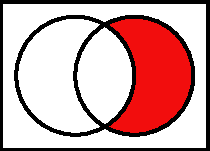
\includegraphics[height=3\baselineskip]{ABSOLUTEPATH/pictures/light-mode/symmetric-difference/definition/BsetminusA.pdf}}}%
                \mkern2.5mu.%
            $}%
        \end{webcompile}%%
        \par\vspace*{\TCBBoxCorrection}
    }%
    %---  End Footnote  ---%
    \[
        U\sdiff V
        \defeq
        (U\setminus V)%
        \cup%
        (V\setminus U).%
    \]%
\end{definition}
\begin{proposition}{Properties of Symmetric Differences}{properties-of-symmetric-differences}%
    Let $X$ be a set.
    \begin{enumerate}
        \item\label{properties-of-symmetric-differences-lack-of-functoriality}\SloganFont{Lack of Functoriality. }The assignment $(U,V)\mapsto U\sdiff V$ \demph{does not} in general define functors
            \[
                \BifunctorialityPeriod{U\sdiff-}{-\sdiff V}{-_{1}\sdiff-_{2}}{(\mathcal{P}(X),\subset)}{(\mathcal{P}(X),\subset)}{(\mathcal{P}(X)\times\mathcal{P}(X),\subset\times\subset)}{(\mathcal{P}(X),\subset)}%
            \]%
        \item\label{properties-of-symmetric-differences-via-unions-and-intersections}\SloganFont{Via Unions and Intersections. }We have%
            \[
                U\sdiff V%
                =%
                (U\cup V)\setminus(U\cap V)%
            \]%
            for each $U,V\in\mathcal{P}(X)$, as in the Venn diagram
            \begin{webcompile}
                \underset{\scalebox{1.0}{$\mkern3.5muU\sdiff V$}}{\raisebox{-0.4\height}{
\includegraphics[height=2\baselineskip]{ABSOLUTEPATH/pictures/light-mode/symmetric-difference/via-unions-and-intersections/Venn0110.pdf}}}%
                \hspace{0.5em}\scalebox{1.5}{$\mathbin{=}$}\hspace{0.6em}%
                \underset{\scalebox{1.0}{$\mkern3.5muU\cup V$}}{\raisebox{-0.4\height}{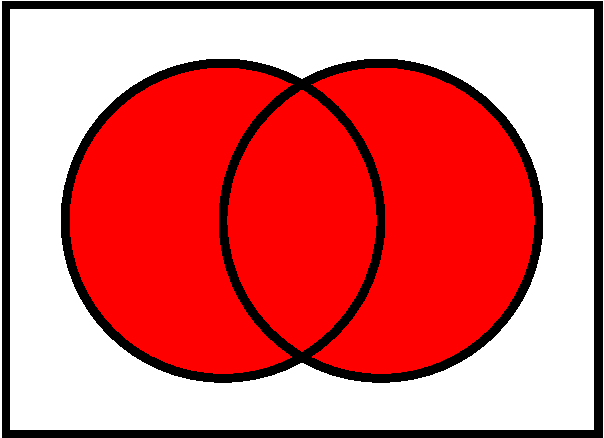
\includegraphics[height=2\baselineskip]{ABSOLUTEPATH/pictures/light-mode/symmetric-difference/via-unions-and-intersections/Venn0111.pdf}}}%
                \hspace{0.5em}\scalebox{1.5}{$\mathbin{\setminus}$}\hspace{0.5em}%
                \underset{\scalebox{1.0}{$\mkern3.5muU\cap V$}}{\raisebox{-0.4\height}{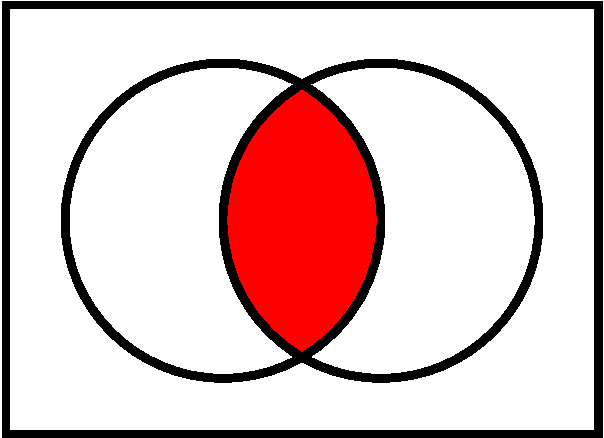
\includegraphics[height=2\baselineskip]{ABSOLUTEPATH/pictures/light-mode/symmetric-difference/via-unions-and-intersections/Venn0001.pdf}}}%
                \mkern2.5mu.%
            \end{webcompile}%%
        \item\label{properties-of-symmetric-differences-symmetric-differences-of-disjoint-sets}\SloganFont{Symmetric Differences of Disjoint Sets. }If $U$ and $V$ are disjoint, then we have
            \[
                U\sdiff V%
                =%
                U\cup V.%
            \]%
        \item\label{properties-of-symmetric-differences-associativity}\SloganFont{Associativity. }The diagram
            \[
                \begin{tikzcd}[row sep={0*\the\DL,between origins}, column sep={0*\the\DL,between origins}, background color=backgroundColor, ampersand replacement=\&]
                    \&[0.30901699437\TwoCmPlusHalf]
                    \&[0.5\TwoCmPlusHalf]
                    \mathcal{P}(X)\times(\mathcal{P}(X)\times\mathcal{P}(X))
                    \&[0.5\TwoCmPlusHalf]
                    \&[0.30901699437\TwoCmPlusHalf]
                    \\[0.58778525229\TwoCmPlusHalf]
                    (\mathcal{P}(X)\times\mathcal{P}(X))\times\mathcal{P}(X)
                    \&[0.30901699437\TwoCmPlusHalf]
                    \&[0.5\TwoCmPlusHalf]
                    \&[0.5\TwoCmPlusHalf]
                    \&[0.30901699437\TwoCmPlusHalf]
                    \mathcal{P}(X)\times\mathcal{P}(X)
                    \\[0.95105651629\TwoCmPlusHalf]
                    \&[0.30901699437\TwoCmPlusHalf]
                    \mathcal{P}(X)\times\mathcal{P}(X)
                    \&[0.5\TwoCmPlusHalf]
                    \&[0.5\TwoCmPlusHalf]
                    \mathcal{P}(X)\mrp{,}
                    \&[0.30901699437\TwoCmPlusHalf]
                    % 1-Arrows
                    % Left Boundary
                    \arrow[from=2-1,to=1-3,"\alpha^{\Sets}_{\mathcal{P}(X),\mathcal{P}(X),\mathcal{P}(X)}"{pos=0.35},isoarrowprime]%
                    \arrow[from=1-3,to=2-5,"{\id_{\mathcal{P}(X)}\times\mathord{\sdiff}}"{pos=0.55},""{name=2}]%
                    \arrow[from=2-5,to=3-4,"\sdiff"{pos=0.425}]%
                    % Right Boundary
                    \arrow[from=2-1,to=3-2,"{\mathord{\sdiff}\times\id_{\mathcal{P}(X)}}"'{pos=0.425}]%
                    \arrow[from=3-2,to=3-4,"\sdiff"']%
                \end{tikzcd}
            \]%
            commutes, i.e.\ we have%
            \[
                (U\sdiff V)\sdiff W
                =
                U\sdiff(V\sdiff W)
            \]%
            for each $U,V,W\in\mathcal{P}(X)$, as in the Venn diagram
            \begin{webcompile}
                \underset{\scalebox{1.0}{$\mkern3.75muU\sdiff V$}}{\raisebox{-0.4\height}{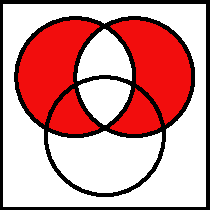
\includegraphics[height=3\baselineskip]{ABSOLUTEPATH/pictures/light-mode/symmetric-difference/associativity/A_sdiff_B.pdf}}}%
                \hspace{0.5em}\scalebox{1.5}{$\mathbin{\sdiff}$}\hspace{0.5em}%
                \underset{\mcp{\scalebox{1.0}{$W$}}}{\raisebox{-0.4\height}{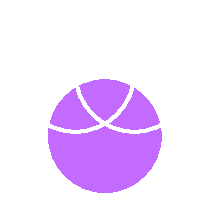
\includegraphics[height=3\baselineskip]{ABSOLUTEPATH/pictures/light-mode/symmetric-difference/associativity/C.pdf}}}%
                \hspace{0.5em}\scalebox{1.5}{$\mathbin{=}$}\hspace{0.3em}%
                \underset{\scalebox{1.0}{$U\sdiff V\sdiff W$}}{\raisebox{-0.4\height}{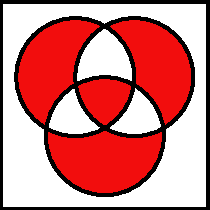
\includegraphics[height=3\baselineskip]{ABSOLUTEPATH/pictures/light-mode/symmetric-difference/associativity/A_sdiff_B_sdiff_C.pdf}}}%
                \hspace{0.2em}\scalebox{1.5}{$\mathbin{=}$}\hspace{0.5em}%
                \underset{\mcp{\scalebox{1.0}{$U$}}}{\raisebox{-0.4\height}{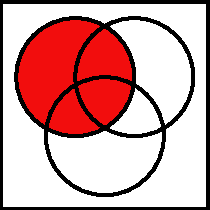
\includegraphics[height=3\baselineskip]{ABSOLUTEPATH/pictures/light-mode/symmetric-difference/associativity/A.pdf}}}%
                \hspace{0.5em}\scalebox{1.5}{$\mathbin{\sdiff}$}\hspace{0.5em}%
                \underset{\scalebox{1.0}{$\mkern4.25muV\sdiff W$}}{\raisebox{-0.4\height}{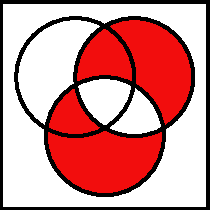
\includegraphics[height=3\baselineskip]{ABSOLUTEPATH/pictures/light-mode/symmetric-difference/associativity/B_sdiff_C.pdf}}}%
                \mkern2.5mu.%
            \end{webcompile}%%
        \item\label{properties-of-symmetric-differences-unitality}\SloganFont{Unitality. }The diagrams
            \begin{scalemath}
                \begin{tikzcd}[row sep={5.0*\the\DL,between origins}, column sep={11.25*\the\DL,between origins}, background color=backgroundColor, ampersand replacement=\&]
                    \pt\times\mathcal{P}(X)
                    \arrow[r,"{[\emptyset]\times\id_{\mathcal{P}(X)}}"]
                    \arrow[rd,"\LUnitor^{\Sets}_{\mathcal{P}(X)}"',isoarrow]
                    \&
                    \mathcal{P}(X)\times\mathcal{P}(X)
                    \arrow[d,"\sdiff"]
                    \\
                    \&
                    \mathcal{P}(X)
                \end{tikzcd}
                \quad
                \begin{tikzcd}[row sep={5.0*\the\DL,between origins}, column sep={11.25*\the\DL,between origins}, background color=backgroundColor, ampersand replacement=\&]
                    \mathcal{P}(X)\times\pt
                    \arrow[r,"{\id_{\mathcal{P}(X)}\times[\emptyset]}"]
                    \arrow[rd,"\RUnitor^{\Sets}_{\mathcal{P}(X)}"',isoarrow]
                    \&
                    \mathcal{P}(X)\times\mathcal{P}(X)
                    \arrow[d,"\sdiff"]
                    \\
                    \&
                    \mathcal{P}(X)
                \end{tikzcd}
            \end{scalemath}
            commute, i.e.\ we have
            \begin{align*}
                U\sdiff\emptyset  &= U,\\
                \emptyset\sdiff U &= U
            \end{align*}
            for each $U\in\mathcal{P}(X)$.
        \item\label{properties-of-symmetric-differences-commutativity}\SloganFont{Commutativity. }The diagram
            \[
                \begin{tikzcd}[row sep={5.0*\the\DL,between origins}, column sep={12.0*\the\DL,between origins}, background color=backgroundColor, ampersand replacement=\&]
                    \mathcal{P}(X)\times\mathcal{P}(X)
                    \arrow[r,"\sigma^{\Sets}_{\mathcal{P}(X),\mathcal{P}(X)}"]
                    \arrow[rd,"\sdiff"']
                    \&
                    \mathcal{P}(X)\times\mathcal{P}(X)
                    \arrow[d,"\sdiff"]
                    \\
                    \&
                    \mathcal{P}(X)
                \end{tikzcd}
            \]%
            commutes, i.e.\ we have
            \[
                U\sdiff V
                =
                V\sdiff U
            \]%
            for each $U,V\in\mathcal{P}(X)$.
        \item\label{properties-of-symmetric-differences-invertibility}\SloganFont{Invertibility. }We have
            \[
                U\sdiff U
                =
                \emptyset
            \]%
            for each $U\in\mathcal{P}(X)$.
        \item\label{properties-of-symmetric-differences-interaction-with-unions}\SloganFont{Interaction With Unions. }We have
            \[
                (U\sdiff V)\cup(V\sdiff T)
                =
                (U\cup V\cup W)\setminus(U\cap V\cap W)
            \]%
            for each $U,V,W\in\mathcal{P}(X)$.
        \item\label{properties-of-symmetric-differences-interaction-with-complements-1}\SloganFont{Interaction With Complements \rmI. }We have
            \[
                U\sdiff U^{\sfc}%
                =
                X%
            \]%
            for each $U\in\mathcal{P}(X)$.
        \item\label{properties-of-symmetric-differences-interaction-with-complements-2}\SloganFont{Interaction With Complements \rmII. }We have
            \begin{align*}
                U\sdiff X &= U^{\sfc},\\%
                X\sdiff U &= U^{\sfc}%
            \end{align*}
            for each $U\in\mathcal{P}(X)$.
        \item\label{properties-of-symmetric-differences-interaction-with-complements-3}\SloganFont{Interaction With Complements \rmIII. }The diagram
            \[
                \begin{tikzcd}[row sep={5.0*\the\DL,between origins}, column sep={8.0*\the\DL,between origins}, background color=backgroundColor, ampersand replacement=\&]
                    \mathcal{P}(X)\times\mathcal{P}(X)
                    \arrow[r,"\sdiff"]
                    \arrow[d,"{(-)^{\sfc}\times(-)^{\sfc}}"']
                    \&
                    \mathcal{P}(X)
                    \arrow[d,"{(-)^{\sfc}}"]
                    \\
                    \mathcal{P}(X)\times\mathcal{P}(X)
                    \arrow[r,"\sdiff"']
                    \&
                    \mathcal{P}(X)
                \end{tikzcd}
            \]%
            commutes, i.e.\ we have
            \[
                U^{\sfc}\sdiff V^{\sfc}%
                =%
                U\sdiff V%
            \]%
            for each $U,V\in\mathcal{P}(X)$.
        \item\label{properties-of-symmetric-differences-transitivity}\SloganFont{\say{Transitivity}. }We have
            \[
                (U\sdiff V)\sdiff(V\sdiff W)%
                =%
               U\sdiff W%
            \]%
            for each $U,V,W\in\mathcal{P}(X)$.
        \item\label{properties-of-symmetric-differences-the-triangle-inequality-for-symmetric-differences}\SloganFont{The Triangle Inequality for Symmetric Differences. }We have
            \[
                U\sdiff W%
                \subset%
                U\sdiff V%
                \cup
                V\sdiff W%
            \]%
            for each $U,V,W\in\mathcal{P}(X)$.
        \item\label{properties-of-symmetric-differences-distributivity-over-intersections}\SloganFont{Distributivity Over Intersections. }We have
            \begin{align*}
                U\cap(V\sdiff W)  &= (U\cap V)\sdiff(U\cap W),\\
                (U\sdiff V)\cap W &= (U\cap W)\sdiff(V\cap W)
            \end{align*}
            for each $U,V,W\in\mathcal{P}(X)$.
        \item\label{properties-of-symmetric-differences-interaction-with-characteristic-functions}\SloganFont{Interaction With Characteristic Functions. }We have
            \[
                \chi_{U\sdiff V}%
                =%
                \chi_{U}%
                +%
                \chi_{V}%
                -%
                2\chi_{U\cap V}%
            \]%
            and thus, in particular, we have
            \[
                \chi_{U\sdiff V}%
                \equiv%
                \chi_{U}+\chi_{V}%
                \mod{2}%
            \]%
            for each $U,V\in\mathcal{P}(X)$.
        \item\label{properties-of-symmetric-differences-bijectivity}\SloganFont{Bijectivity. }Given $U,V\in\mathcal{P}(X)$, the maps
            \begin{align*}
                U\sdiff-  &\colon \mathcal{P}(X) \to \mathcal{P}(X),\\
                -\sdiff V &\colon \mathcal{P}(X) \to \mathcal{P}(X)
            \end{align*}
            are self-inverse bijections. Moreover, the map
            \begin{webcompile}
                \begin{tikzcd}[row sep=0.0*\the\DL, column sep=1.0*\the\DL, background color=backgroundColor, ampersand replacement=\&]
                    \mathcal{P}(X)
                    \arrow[r]
                    \&
                    \mathcal{P}(X)
                    \\
                    C
                    \arrow[r, mapsto]
                    \&
                    C\sdiff(U\sdiff V)%
                \end{tikzcd}
            \end{webcompile}%
            is a bijection of $\mathcal{P}(X)$ onto itself sending $U$ to $V$ and $V$ to $U$.
        \item\label{properties-of-symmetric-differences-interaction-with-powersets-and-groups}\SloganFont{Interaction With Powersets and Groups. }Let $X$ be a set.
            \begin{enumerate}
                \item\label{properties-of-symmetric-differences-interaction-with-powersets-and-groups-a}The quadruple $(\mathcal{P}(X),\sdiff,\emptyset,\id_{\mathcal{P}(X)})$ is an abelian group.%
                    %--- Begin Footnote ---%
                    \footnote{%
                        Here are some examples:
                        \begin{enumerate}
                            \item\label{proof-of-properties-of-symmetric-differences-interaction-with-powersets-and-groups-a-1}When $X=\emptyset$, we have an isomorphism of groups between $\mathcal{P}(\emptyset)$ and the trivial group:
                                \[
                                    (\mathcal{P}(\emptyset),\sdiff,\emptyset,\id_{\mathcal{P}(\emptyset)})
                                    \cong
                                    \pt.
                                \]%
                            \item\label{proof-of-properties-of-symmetric-differences-interaction-with-powersets-and-groups-a-2}When $X=\pt$, we have an isomorphism of groups between $\mathcal{P}(\pt)$ and $\Zn{2}$:
                                \[
                                    (\mathcal{P}(\pt),\sdiff,\emptyset,\id_{\mathcal{P}(\pt)})
                                    \cong
                                    \Zn{2}.
                                \]%
                            \item\label{proof-of-properties-of-symmetric-differences-interaction-with-powersets-and-groups-a-3}When $X=\{0,1\}$, we have an isomorphism of groups between $\mathcal{P}(\{0,1\})$ and $\Zn{2}\times\Zn{2}$:
                                \[
                                    (\mathcal{P}(\{0,1\}),\sdiff,\emptyset,\id_{\mathcal{P}(\{0,1\})})
                                    \cong
                                    \Zn{2}\times\Zn{2}.
                                \]%
                        \end{enumerate}
                        \par\vspace*{\TCBBoxCorrection}
                    }%
                    %---  End Footnote  ---%
                \item\label{properties-of-symmetric-differences-interaction-with-powersets-and-groups-b}Every element of $\mathcal{P}(X)$ has order $2$ with respect to $\sdiff$, and thus $\mathcal{P}(X)$ is a \emph{Boolean group} (i.e.\ an abelian $2$-group).
            \end{enumerate}
        \item\label{properties-of-symmetric-differences-interaction-with-powersets-and-vector-spaces-1}\SloganFont{Interaction With Powersets and Vector Spaces \rmI. }The pair $(\mathcal{P}(X),\alpha_{\mathcal{P}(X)})$ consisting of
            \begin{itemize}
                \item The group $\mathcal{P}(X)$ of \cref{properties-of-symmetric-differences-interaction-with-powersets-and-groups};
                \item The map $\alpha_{\mathcal{P}(X)}\colon\F_{2}\times\mathcal{P}(X)\to\mathcal{P}(X)$ defined by
                    \begin{align*}
                        0\cdot U &\defeq \emptyset,\\
                        1\cdot U &\defeq U;
                    \end{align*}
            \end{itemize}
            is an $\F_{2}$-vector space.
        \item\label{properties-of-symmetric-differences-interaction-with-powersets-and-vector-spaces-2}\SloganFont{Interaction With Powersets and Vector Spaces \rmII. }If $X$ is finite, then:
            \begin{enumerate}
                \item\label{properties-of-symmetric-differences-interaction-with-powersets-and-vector-spaces-2-a}The set of singletons sets on the elements of $X$ forms a basis for the $\F_{2}$-vector space $(\mathcal{P}(X),\alpha_{\mathcal{P}(X)})$ of \cref{properties-of-symmetric-differences-interaction-with-powersets-and-vector-spaces-1}.
                \item\label{properties-of-symmetric-differences-interaction-with-powersets-and-vector-spaces-2-b}We have
                    \[
                        \dim(\mathcal{P}(X))%
                        =%
                        \Card{X}.%
                    \]%
            \end{enumerate}
        \item\label{properties-of-symmetric-differences-interaction-with-powersets-and-rings}\SloganFont{Interaction With Powersets and Rings. }The quintuple $(\mathcal{P}(X),\sdiff,\cap,\emptyset,X)$ is a commutative ring.%
            %--- Begin Footnote ---%
            \footnote{%
                \textdbend\SloganFont{Warning: }The analogous statement replacing intersections by unions (i.e.\ that the quintuple $(\mathcal{P}(X),\sdiff,\cup,\emptyset,X)$ is a ring) is false, however. See \cite{proof-wiki:symmetric-difference-with-union-does-not-form-ring} for a proof.
                \par\vspace*{\TCBBoxCorrection}
            }%
            %---  End Footnote  ---%
        %\item\label{properties-of-symmetric-differences-}\SloganFont{. }
        \item\label{properties-of-symmetric-differences-interaction-with-direct-images}\SloganFont{Interaction With Direct Images. }We have a natural transformation
            \[
                \begin{tikzcd}[row sep={5.0*\the\DL,between origins}, column sep={11.5*\the\DL,between origins}, background color=backgroundColor, ampersand replacement=\&]
                    \mathcal{P}(X)^{\op}\times\mathcal{P}(X)
                    \arrow[r,"f^{\op}_{!}\times f_{!}"]
                    \arrow[d,"\sdiff"']
                    \&
                    \mathcal{P}(Y)^{\op}\times\mathcal{P}(Y)
                    \arrow[d,"\sdiff"]
                    \\
                    \mathcal{P}(X)
                    \arrow[r,"f_{!}"']
                    \&
                    \mathcal{P}(Y)
                    % 2-Arrows
                    \arrow[from=1-2,to=2-1,"\scalebox{1.5}{$\supset$}"{sloped,description},phantom,shorten <= 0.5*\the\DL,shorten >= 0.625*\the\DL,Rightarrow,pos=0.5]%
                \end{tikzcd}
            \]%
            with components
            \[
                f_{!}(U)\sdiff f_{!}(V)%
                \subset%
                f_{!}(U\sdiff V)%
            \]%
            indexed by $U,V\in\mathcal{P}(X)$.
        \item\label{properties-of-symmetric-differences-interaction-with-inverse-images}\SloganFont{Interaction With Inverse Images. }The diagram
            \[
                \begin{tikzcd}[row sep={5.0*\the\DL,between origins}, column sep={13.0*\the\DL,between origins}, background color=backgroundColor, ampersand replacement=\&]
                    \mathcal{P}(Y)^{\op}\times\mathcal{P}(Y)
                    \arrow[r,"f^{\op,-1}\times f^{-1}"]
                    \arrow[d,"\sdiff"']
                    \&
                    \mathcal{P}(X)^{\op}\times\mathcal{P}(X)
                    \arrow[d,"\sdiff"]
                    \\
                    \mathcal{P}(Y)
                    \arrow[r,"f^{-1}"']
                    \&
                    \mathcal{P}(X)
                \end{tikzcd}
            \]%
            i.e.\ we have
            \[
                f^{-1}(U)\sdiff f^{-1}(V)%
                =%
                f^{-1}(U\sdiff V)%
            \]%
            for each $U,V\in\mathcal{P}(Y)$.
        \item\label{properties-of-symmetric-differences-interaction-with-codirect-images}\SloganFont{Interaction With Codirect Images. }We have a natural transformation
            \[
                \begin{tikzcd}[row sep={5.0*\the\DL,between origins}, column sep={11.5*\the\DL,between origins}, background color=backgroundColor, ampersand replacement=\&]
                    \mathcal{P}(X)^{\op}\times\mathcal{P}(X)
                    \arrow[r,"f^{\op}_{*}\times f_{*}"]
                    \arrow[d,"\sdiff"']
                    \&
                    \mathcal{P}(Y)^{\op}\times\mathcal{P}(Y)
                    \arrow[d,"\sdiff"]
                    \\
                    \mathcal{P}(X)
                    \arrow[r,"f_{*}"']
                    \&
                    \mathcal{P}(Y)
                    % 2-Arrows
                    \arrow[from=2-1,to=1-2,"\scalebox{1.5}{$\supset$}"{sloped,description},phantom,shorten <= 0.5*\the\DL,shorten >= 0.625*\the\DL,Rightarrow,pos=0.5]%
                \end{tikzcd}
            \]%
            with components
            \[
                f_{*}(U\sdiff V)%
                \subset%
                f_{*}(U)\sdiff f_{*}(V)%
            \]%
            indexed by $U,V\in\mathcal{P}(X)$.
    \end{enumerate}
\end{proposition}
\begin{Proof}{Proof of \cref{properties-of-symmetric-differences}}%
    \FirstProofBox{\cref{properties-of-symmetric-differences-lack-of-functoriality}: Lack of Functoriality}%
    Let $X = \{0,1\}, U = \{0\}$. Then $\emptyset \subset U$, but
    $U \sdiff \emptyset = U \nsubset \emptyset = U \sdiff U$ from \cref{properties-of-symmetric-differences-unitality} and \cref{properties-of-symmetric-differences-invertibility}. This gives a counterexample to the first statement. By using \cref{properties-of-symmetric-differences-commutativity}, we can adapt it to the second and third statement.

    \ProofBox{\cref{properties-of-symmetric-differences-via-unions-and-intersections}: Via Unions and Intersections}%
    See \cite{proof-wiki:equivalence-of-definitions-of-symmetric-difference}.

    \ProofBox{\cref{properties-of-symmetric-differences-symmetric-differences-of-disjoint-sets}: Symmetric Differences of Disjoint Sets}%
    Since $U$ and $V$ are disjoint, we have $U\cap V=\emptyset$, and therefore we have
    \begin{align*}
        U\sdiff V &= (U\cup V)\setminus(U\cap V)\\
                  &= (U\cup V)\setminus\emptyset\\
                  &= U\cup V,
    \end{align*}
    where we've used \cref{properties-of-symmetric-differences-via-unions-and-intersections} and \cref{properties-of-differences-right-unitality} of \cref{properties-of-differences}.

    \ProofBox{\cref{properties-of-symmetric-differences-associativity}: Associativity}%
    See \cite{proof-wiki:symmetric-difference-is-associative}.

    \ProofBox{\cref{properties-of-symmetric-differences-unitality}: Unitality}%
    This follows from \cref{properties-of-symmetric-differences-commutativity} and \cite{proof-wiki:symmetric-difference-with-empty-set}.

    \ProofBox{\cref{properties-of-symmetric-differences-commutativity}: Commutativity}%
    See \cite{proof-wiki:symmetric-difference-is-commutative}.

    \ProofBox{\cref{properties-of-symmetric-differences-invertibility}: Invertibility}%
    See \cite{proof-wiki:symmetric-difference-with-self-is-empty-set}.

    \ProofBox{\cref{properties-of-symmetric-differences-interaction-with-unions}: Interaction With Unions}%
    See \cite{proof-wiki:union-of-symmetric-differences}.

    \ProofBox{\cref{properties-of-symmetric-differences-interaction-with-complements-1}: Interaction With Complements \rmI}%
    See \cite{proof-wiki:symmetric-difference-with-complement}.

    \ProofBox{\cref{properties-of-symmetric-differences-interaction-with-complements-2}: Interaction With Complements \rmII}%
    This follows from \cref{properties-of-symmetric-differences-commutativity} and \cite{proof-wiki:symmetric-difference-with-universe}.

    \ProofBox{\cref{properties-of-symmetric-differences-interaction-with-complements-3}: Interaction With Complements \rmIII}%
    See \cite{proof-wiki:symmetric-difference-of-complements}.

    \ProofBox{\cref{properties-of-symmetric-differences-transitivity}: \say{Transitivity}}%
    We have
    \begin{palign}
        $(U\sdiff V)\sdiff(V\sdiff W)$ & $\mathord{=}$ & $U\sdiff(V\sdiff(V\sdiff W))$  & {\small(by \cref{properties-of-symmetric-differences-associativity})}\\
                                       & $\mathord{=}$ & $U\sdiff((V\sdiff V)\sdiff W)$ & {\small(by \cref{properties-of-symmetric-differences-associativity})}\\
                                       & $\mathord{=}$ & $U\sdiff(\emptyset\sdiff W)$   & {\small(by \cref{properties-of-symmetric-differences-invertibility})}\\
                                       & $\mathord{=}$ & $U\sdiff W$.                   & {\small(by \cref{properties-of-symmetric-differences-unitality})}
    \end{palign}
    This finishes the proof.

    \ProofBox{\cref{properties-of-symmetric-differences-the-triangle-inequality-for-symmetric-differences}: The Triangle Inequality for Symmetric Differences}%
    This follows from \cref{properties-of-symmetric-differences-transitivity,properties-of-symmetric-differences-via-unions-and-intersections}.

    \ProofBox{\cref{properties-of-symmetric-differences-distributivity-over-intersections}: Distributivity Over Intersections}%
    See \cite{proof-wiki:intersection-distributes-over-symmetric-difference}.

    \ProofBox{\cref{properties-of-symmetric-differences-interaction-with-characteristic-functions}: Interaction With Characteristic Functions}%
    See \cite{proof-wiki:characteristic-function-of-symmetric-difference}.

    \ProofBox{\cref{properties-of-symmetric-differences-bijectivity}: Bijectivity}%
    \begin{itemize}
        \item We show that
            \[%
                (U\sdiff-)%
                \colon%
                \mathcal{P}(X)%
                \to%
                \mathcal{P}(X)%
            \]%
            is self-inverse.

            Let $W \in \mathcal{P}(X)$. Then,
            \begin{palign}
              $U \sdiff (U \sdiff W)$ & $\mathord{=}$ & $(U \sdiff U) \sdiff W$ & {\small(by \cref{properties-of-symmetric-differences-associativity})}\\
              & $\mathord{=}$ & $\emptyset \sdiff W$ & {\small(by \cref{properties-of-symmetric-differences-invertibility})}\\
              & $\mathord{=}$ & $W$. & {\small(by \cref{properties-of-symmetric-differences-unitality})}
            \end{palign}
      \item By \cref{properties-of-symmetric-differences-commutativity}, $(- \sdiff V) = (V \sdiff -)$, hence the former is also self-inverse by the first point.
      \item The map $- \sdiff (U \sdiff V)$ is a bijection as a special case of the second point.
            From the first two points and \cref{properties-of-symmetric-differences-commutativity}, we get
            \[ U \sdiff (U \sdiff V) = V,\ V \sdiff (U \sdiff V) = V \sdiff (V \sdiff U) = U. \]
            Hence the function maps $U$ to $V$ and $V$ to $U$.
    \end{itemize}

    \ProofBox{\cref{properties-of-symmetric-differences-interaction-with-powersets-and-groups}: Interaction With Powersets and Groups}%
    \cref{properties-of-symmetric-differences-interaction-with-powersets-and-groups-a} follows from \cref{properties-of-symmetric-differences-associativity,properties-of-symmetric-differences-unitality,properties-of-symmetric-differences-invertibility,properties-of-symmetric-differences-commutativity}, while \cref{properties-of-symmetric-differences-interaction-with-powersets-and-groups-b} follows from \cref{properties-of-symmetric-differences-invertibility}.%
    %--- Begin Footnote ---%
    \footnote{%
        \SloganFont{Reference: }\cite{proof-wiki:symmetric-difference-on-power-set-forms-abelian-group}.
    }%
    %---  End Footnote  ---%

    \ProofBox{\cref{properties-of-symmetric-differences-interaction-with-powersets-and-vector-spaces-1}: Interaction With Powersets and Vector Spaces \rmI}%
    See \cite{MSE2719059}.

    \ProofBox{\cref{properties-of-symmetric-differences-interaction-with-powersets-and-vector-spaces-2}: Interaction With Powersets and Vector Spaces \rmII}%
    See \cite{MSE2719059}.

    \ProofBox{\cref{properties-of-symmetric-differences-interaction-with-powersets-and-rings}: Interaction With Powersets and Rings}%
    This follows from \cref{properties-of-binary-intersections-annihilation-with-the-empty-set,properties-of-binary-intersections-interaction-with-powersets-and-monoids-with-zero} of \cref{properties-of-binary-intersections} and \cref{properties-of-symmetric-differences-distributivity-over-intersections,properties-of-symmetric-differences-interaction-with-powersets-and-groups}.%
    %--- Begin Footnote ---%
    \footnote{%
        \SloganFont{Reference: }\cite{proof-wiki:symmetric-difference-with-intersection-forms-ring}.
        \par\vspace*{\TCBBoxCorrection}
    }%
    %---  End Footnote  ---%

    \ProofBox{\cref{properties-of-symmetric-differences-interaction-with-direct-images}: Interaction With Direct Images}%
    This is a repetition of \cref{properties-of-direct-images-i-interaction-with-symmetric-differences} of \cref{properties-of-direct-images-i} and is proved there.

    \ProofBox{\cref{properties-of-symmetric-differences-interaction-with-inverse-images}: Interaction With Inverse Images}%
    This is a repetition of \cref{properties-of-inverse-images-i-interaction-with-symmetric-differences} of \cref{properties-of-inverse-images-i} and is proved there.

    \ProofBox{\cref{properties-of-symmetric-differences-interaction-with-codirect-images}: Interaction With Codirect Images}%
    This is a repetition of \cref{properties-of-codirect-images-i-interaction-with-symmetric-differences} of \cref{properties-of-codirect-images-i} and is proved there.
\end{Proof}
\section{Characteristic Functions}\label{section-characteristic-functions}
\subsection{The Characteristic Function of a Subset}\label{subsection-the-characteristic-function-of-a-subset}
Let $X$ be a set and let $U\in\mathcal{P}(X)$.
\begin{definition}{The Characteristic Function of a Subset}{the-characteristic-function-of-a-subset}%
    The \index[set-theory]{characteristic function!of a subset}\textbf{characteristic function of $U$}%
    %--- Begin Footnote ---%
    \footnote{%
        \SloganFont{Further Terminology: }Also called the \index[set-theory]{indicator function|see {characteristic function}}\textbf{indicator function of $U$}.
    } %
    %---  End Footnote  ---%
    is the function\index[notation]{chiU@$\chi_{U}$}$\chi_{U}\colon X\to\TTV$%
    %--- Begin Footnote ---%
    \footnote{%
        \SloganFont{Further Notation: }Also written \index[notation]{chiXU@$\chi_{X}(U,-)$}$\chi_{X}(U,-)$ or \index[notation]{chiXU@$\chi_{X}(-,U)$}$\chi_{X}(-,U)$.
        \par\vspace*{\TCBBoxCorrection}
    } %
    %---  End Footnote  ---%
    defined by
    \[
        \chi_{U}(x)
        \defeq
        \begin{cases}
            \true  &\text{if $x\in U$,}\\
            \false &\text{if $x\nin U$}
        \end{cases}
    \]%
    for each $x\in X$.
\end{definition}
\begin{remark}{Characteristic Functions of Subsets as Decategorifications of Presheaves}{characteristic-functions-of-subsets-as-decategorifications-of-presheaves}%
    Under the analogy that $\TTV$ should be the $(-1)$-categorical analogue of $\Sets$, we may view a function
    \[
        f\colon X\to\TTV%
    \]%
    as a decategorification of presheaves and copresheaves%
    \begin{gather*}
        \SheafFont{F} \colon \CatFont{C}^{\op} \to \Sets,\\%
        F             \colon \CatFont{C}       \to \Sets.%
    \end{gather*}
    The characteristic functions $\chi_{U}$ of the subsets of $X$ are then the primordial examples of such functions (and, in fact, all of them).
\end{remark}
\begin{notation}{Further Notation for Characteristic Functions}{further-notation-for-characteristic-functions}%
    We will often employ the bijection $\TTV\cong\{0,1\}$ to make use of the arithmetical operations defined on $\{0,1\}$ when disucssing characteristic functions.

    \indent Examples of this include \cref{properties-of-characteristic-functions-of-subsets-interaction-with-unions-1,properties-of-characteristic-functions-of-subsets-interaction-with-unions-2,properties-of-characteristic-functions-of-subsets-interaction-with-intersections-1,properties-of-characteristic-functions-of-subsets-interaction-with-intersections-2,properties-of-characteristic-functions-of-subsets-interaction-with-differences,properties-of-characteristic-functions-of-subsets-interaction-with-complements,properties-of-characteristic-functions-of-subsets-interaction-with-symmetric-differences,properties-of-characteristic-functions-of-subsets-interaction-with-internal-homs} of \cref{properties-of-characteristic-functions-of-subsets} below.
\end{notation}
\begin{proposition}{Properties of Characteristic Functions of Subsets}{properties-of-characteristic-functions-of-subsets}%
    Let $X$ be a set.
    \begin{enumerate}
        \item\label{properties-of-characteristic-functions-of-subsets-functionality}\SloganFont{Functionality. }The assignment $U\mapsto\chi_{U}$ defines a function
            \[
                \chi_{(-)}%
                \colon%
                \mathcal{P}(X)%
                \to%
                \Sets(X,\TTV).%
            \]%
        \item\label{properties-of-characteristic-functions-of-subsets-bijectivity}\SloganFont{Bijectivity. }The function $\chi_{(-)}$ from \cref{properties-of-characteristic-functions-of-subsets-functionality} is bijective.
        \item\label{properties-of-characteristic-functions-of-subsets-naturality}\SloganFont{Naturality. }The collection
            \[
                \{%
                    \chi_{(-)}%
                    \colon%
                    \mathcal{P}(X)%
                    \to%
                    \Sets(X,\TTV)%
                \}_{X\in\Obj(\Sets)}%
            \]%
            defines a natural isomorphism between $\mathcal{P}^{-1}$ and $\Sets(-,\TTV)$. In particular, given a function $f\colon X\to Y$, the diagram
            \[
                \begin{tikzcd}[row sep={5.0*\the\DL,between origins}, column sep={9.0*\the\DL,between origins}, background color=backgroundColor, ampersand replacement=\&]
                    \mathcal{P}(Y)
                    \arrow[r,"f^{-1}"]
                    \arrow[d,bigisoarrow,"{\chi_{(-)}}"']
                    \&
                    \mathcal{P}(X)
                    \arrow[d,bigisoarrowprime,"{\chi_{(-)}}"]
                    \\
                    \Sets(Y,\TTV)
                    \arrow[r,"f^{*}"']
                    \&
                    \Sets(X,\TTV)
                \end{tikzcd}
            \]%
            commutes, i.e.\ we have
            \[
                \chi_{V}\circ f%
                =%
                \chi_{f^{-1}(V)}%
            \]%
            for each $V\in\mathcal{P}(Y)$.
        \item\label{properties-of-characteristic-functions-of-subsets-interaction-with-unions-1}\SloganFont{Interaction With Unions \rmI. }We have
            \[
                \chi_{U\cup V}%
                =%
                \max(\chi_{U},\chi_{V})%
            \]%
            for each $U,V\in\mathcal{P}(X)$.
        \item\label{properties-of-characteristic-functions-of-subsets-interaction-with-unions-2}\SloganFont{Interaction With Unions \rmII. }We have
            \[
                \chi_{U\cup V}%
                =%
                \chi_{U}+\chi_{V}-\chi_{U\cap V}%
            \]%
            for each $U,V\in\mathcal{P}(X)$.
        \item\label{properties-of-characteristic-functions-of-subsets-interaction-with-intersections-1}\SloganFont{Interaction With Intersections \rmI. }We have
            \[
                \chi_{U\cap V}%
                =%
                \chi_{U}\chi_{V}%
            \]%
            for each $U,V\in\mathcal{P}(X)$.
        \item\label{properties-of-characteristic-functions-of-subsets-interaction-with-intersections-2}\SloganFont{Interaction With Intersections \rmII. }We have
            \[
                \chi_{U\cap V}%
                =%
                \min(\chi_{U},\chi_{V})%
            \]%
            for each $U,V\in\mathcal{P}(X)$.
        \item\label{properties-of-characteristic-functions-of-subsets-interaction-with-differences}\SloganFont{Interaction With Differences. }We have
            \[
                \chi_{U\setminus V}%
                =%
                \chi_{U}%
                -%
                \chi_{U\cap V}%
            \]%
            for each $U,V\in\mathcal{P}(X)$.
        \item\label{properties-of-characteristic-functions-of-subsets-interaction-with-complements}\SloganFont{Interaction With Complements. }We have
            \[
                \chi_{U^{\sfc}}%
                =%
                1-\chi_{U}%
            \]%
            for each $U\in\mathcal{P}(X)$.
        \item\label{properties-of-characteristic-functions-of-subsets-interaction-with-symmetric-differences}\SloganFont{Interaction With Symmetric Differences. }We have
            \[
                \chi_{U\sdiff V}%
                =%
                \chi_{U}%
                +%
                \chi_{V}%
                -%
                2\chi_{U\cap V}%
            \]%
            and thus, in particular, we have
            \[
                \chi_{U\sdiff V}%
                \equiv%
                \chi_{U}+\chi_{V}%
                \mod{2}%
            \]%
            for each $U,V\in\mathcal{P}(X)$.
        \item\label{properties-of-characteristic-functions-of-subsets-interaction-with-internal-homs}\SloganFont{Interaction With Internal Homs. }We have
            \[
                \chi_{[U,V]_{\mathcal{P}(X)}}%
                =%
                \max(1-\chi_{U}\mmod{2},\chi_{V})
            \]%
            for each $U,V\in\mathcal{P}(X)$.
    \end{enumerate}
\end{proposition}
\begin{Proof}{Proof of \cref{properties-of-characteristic-functions-of-subsets}}%
    \FirstProofBox{\cref{properties-of-characteristic-functions-of-subsets-functionality}: Functionality}%
    There is nothing to prove.

    \ProofBox{\cref{properties-of-characteristic-functions-of-subsets-bijectivity}: Bijectivity}%
    We proceed in three steps:
    \begin{enumerate}
        \item\label{proof-of-properties-of-characteristic-functions-of-subsets-bijectivity-1}\SloganFont{The Inverse of $\chi_{(-)}$. }The inverse of $\chi_{(-)}$ is the map
            \[
                \Phi%
                \colon
                \Sets(X,\TTV)
                \isorightarrow
                \mathcal{P}(X),
            \]%
            defined by
            \begin{align*}
                \Phi(f) &\defeq U_{f}\\
                        &\defeq f^{-1}(\true)\\
                        &\eqdef \{%
                                    x\in X%
                                    \ \middle|\ %
                                    f(x)=\true%
                                \}%
            \end{align*}
            for each $f\in\Sets(X,\TTV)$.
        \item\label{proof-of-properties-of-characteristic-functions-of-subsets-bijectivity-2}\SloganFont{Invertibility \rmI. }We have
            \begin{align*}
                [\Phi\circ\chi_{(-)}](U) &\eqdef \Phi(\chi_{U})\\
                                         &\eqdef \chi^{-1}_{U}(\true)\\
                                         &\eqdef \{x\in X\ \middle|\ \chi_{U}(x)=\true\}\\
                                         &\eqdef \{x\in X\ \middle|\ x\in U\}\\
                                         &=      U\\
                                         &\eqdef [\id_{\mathcal{P}(X)}](U)
            \end{align*}
            for each $U\in\mathcal{P}(X)$. Thus, we have
            \[
                \Phi\circ\chi_{(-)}%
                =%
                \id_{\mathcal{P}(X)}.%
            \]%
        \item\label{proof-of-properties-of-characteristic-functions-of-subsets-bijectivity-3}\SloganFont{Invertibility \rmII. }We have
            \begin{align*}
                [\chi_{(-)}\circ\Phi](U) &\eqdef \chi_{\Phi(f)}\\
                                         &\eqdef \chi_{f^{-1}(\true)}\\
                                         &\eqdef \llbracket x\mapsto\begin{cases}\true &\text{if $x\in f^{-1}(\true)$}\\\false &\text{otherwise}\end{cases}\rrbracket\\
                                         &=      \llbracket x\mapsto f(x)\rrbracket\\
                                         &=      f\\
                                         &\eqdef [\id_{\Sets(X,\TTV)}](f)
            \end{align*}
            for each $f\in\Sets(X,\TTV)$. Thus, we have
            \[
                \chi_{(-)}\circ\Phi%
                =%
                \id_{\Sets(X,\TTV)}.%
            \]%
    \end{enumerate}
    This finishes the proof.

    \ProofBox{\cref{properties-of-characteristic-functions-of-subsets-naturality}: Naturality}%
    We proceed in two steps:
    \begin{enumerate}
        \item\label{proof-of-properties-of-characteristic-functions-of-subsets-naturality-1}\SloganFont{Naturality of $\chi_{(-)}$. }We have
            \begin{align*}
                [\chi_{V}\circ f](v) &\eqdef \chi_{V}(f(v))\\%
                                     &=      \begin{cases}
                                                 \true  &\text{if $f(v)\in V$,}\\
                                                 \false &\text{otherwise}
                                             \end{cases}\\
                                     &=      \begin{cases}
                                                 \true  &\text{if $v\in f^{-1}(V)$,}\\
                                                 \false &\text{otherwise}
                                             \end{cases}\\
                                     &\eqdef \chi_{f^{-1}(V)}(v)%
            \end{align*}
            for each $v\in V$.
        \item\label{proof-of-properties-of-characteristic-functions-of-subsets-naturality-2}\SloganFont{Naturality of $\Phi$. }Since $\chi_{(-)}$ is natural and a componentwise inverse to $\Phi$, it follows from \ChapterRef{\ChapterCategories, \cref{categories:properties-of-natural-isomorphisms-componentwise-inverses-of-natural-transformations-assemble-into-natural-transformations} of \cref{categories:properties-of-natural-isomorphisms}}{\cref{properties-of-natural-isomorphisms-componentwise-inverses-of-natural-transformations-assemble-into-natural-transformations} of \cref{properties-of-natural-isomorphisms}} that $\Phi$ is also natural in each argument.
    \end{enumerate}
    This finishes the proof.

    \ProofBox{\cref{properties-of-characteristic-functions-of-subsets-interaction-with-unions-1}: Interaction With Unions \rmI}%
    This is a repetition of \cref{properties-of-binary-unions-interaction-with-characteristic-functions-1} of \cref{properties-of-binary-unions} and is proved there.

    \ProofBox{\cref{properties-of-characteristic-functions-of-subsets-interaction-with-unions-2}: Interaction With Unions \rmII}%
    This is a repetition of \cref{properties-of-binary-unions-interaction-with-characteristic-functions-2} of \cref{properties-of-binary-unions} and is proved there.

    \ProofBox{\cref{properties-of-characteristic-functions-of-subsets-interaction-with-intersections-1}: Interaction With Intersections \rmI}%
    This is a repetition of \cref{properties-of-binary-intersections-interaction-with-characteristic-functions-1} of \cref{properties-of-binary-intersections} and is proved there.

    \ProofBox{\cref{properties-of-characteristic-functions-of-subsets-interaction-with-intersections-2}: Interaction With Intersections \rmII}%
    This is a repetition of \cref{properties-of-binary-intersections-interaction-with-characteristic-functions-2} of \cref{properties-of-binary-intersections} and is proved there.

    \ProofBox{\cref{properties-of-characteristic-functions-of-subsets-interaction-with-differences}: Interaction With Differences}%
    This is a repetition of \cref{properties-of-differences-interaction-with-characteristic-functions} of \cref{properties-of-differences} and is proved there.

    \ProofBox{\cref{properties-of-characteristic-functions-of-subsets-interaction-with-complements}: Interaction With Complements}%
    This is a repetition of \cref{properties-of-complements-interaction-with-characteristic-functions} of \cref{properties-of-complements} and is proved there.

    \ProofBox{\cref{properties-of-characteristic-functions-of-subsets-interaction-with-symmetric-differences}: Interaction With Symmetric Differences}%
    This is a repetition of \cref{properties-of-symmetric-differences-interaction-with-characteristic-functions} of \cref{properties-of-symmetric-differences} and is proved there.

    \ProofBox{\cref{properties-of-characteristic-functions-of-subsets-interaction-with-internal-homs}: Interaction With Internal Homs}%
    This is a repetition of \cref{properties-of-internal-homs-of-powersets-interaction-with-characteristic-functions} of \cref{properties-of-internal-homs-of-powersets} and is proved there.
\end{Proof}
\begin{remark}{Powersets as Sets of Functions and Un/Straightening}{powersets-as-sets-of-functions-and-un-straightening}%
    The bijection
    \[
        \mathcal{P}(X)%
        \cong%
        \Sets(X,\TTV)%
    \]%
    of \cref{properties-of-characteristic-functions-of-subsets-bijectivity} of \cref{properties-of-characteristic-functions-of-subsets}, which
    \begin{itemize}
        \item Takes a subset $U\hookrightarrow X$ of $X$ and \emph{straightens} it to a function $\chi_{U}\colon X\to\TV$;
        \item Takes a function $f\colon X\to\TV$ and \emph{unstraightens} it to a subset $f^{-1}(\true)\hookrightarrow X$ of $X$;
    \end{itemize}
    may be viewed as the $(-1)$-categorical version of the 0-categorical un/straightening isomorphism between indexed and fibred sets
    \[
        \underbrace{\FibSets_{X}}_{\eqdef\Sets_{/X}}%
        \cong%
        \underbrace{\ISets_{X}}_{\eqdef\Fun(X_{\disc},\Sets)}%
    \]%
    of \ChapterRef{\ChapterUnStraighteningForIndexedAndFibredSets, \cref{un-straightening-for-indexed-and-fibred-sets:theorem-un-straightening-for-indexed-and-fibred-sets}}{\cref{theorem-un-straightening-for-indexed-and-fibred-sets}}. Here we view:
    \begin{itemize}
        \item Subsets $U\hookrightarrow X$ as being analogous to $X$-fibred sets $\phi_{X}\colon A\to X$.
        \item Functions $f\colon X\to\TTV$ as being analogous to $X$-indexed sets $A\colon X_{\disc}\to\Sets$.
    \end{itemize}
\end{remark}
\subsection{The Characteristic Function of a Point}\label{subsection-the-characteristic-function-of-a-point}
Let $X$ be a set and let $x\in X$.
\begin{definition}{The Characteristic Function of a Point}{the-characteristic-function-of-a-point}%
    The \index[set-theory]{characteristic function!of an element}\textbf{characteristic function of $x$} is the function\index[notation]{chix@$\chi_{x}$}%
    %--- Begin Footnote ---%
    \footnote{%
        \SloganFont{Further Notation: }Also written \index[notation]{chix@$\chi^{x}$}$\chi^{x}$, \index[notation]{chiXx@$\chi_{X}(x,-)$}$\chi_{X}(x,-)$, or \index[notation]{chiXU@$\chi_{X}(-,x)$}$\chi_{X}(-,x)$.
    }%
    %---  End Footnote  ---%
    \[%
        \chi_{x}%
        \colon%
        X%
        \to%
        \TTV%
    \]%
    defined by%
    \[
        \chi_{x}
        \defeq
        \chi_{\{x\}},%
    \]%
    so we have%
    \[
        \chi_{x}(y)
        \eqdef%
        \begin{cases}
            \true  &\text{if $x=y$,}\\
            \false &\text{if $x\neq y$}
        \end{cases}
    \]%
    for each $y\in X$.
\end{definition}
\begin{remark}{Characteristic Functions of Points as Decategorifications of Representable Presheaves}{characteristic-functions-of-points-as-decategorifications-of-representable-presheaves}%
    Expanding upon \cref{characteristic-functions-of-subsets-as-decategorifications-of-presheaves}, we may think of the characteristic function%
    \[%
        \chi_{x}%
        \colon%
        X%
        \to%
        \TTV%
    \]%
    of an \emph{element} $x$ of $X$ as a decategorification of the representable presheaf and of the representable copresheaf
    \begin{align*}
        h_{X} &\colon \CatFont{C}^{\op} \to \Sets,\\%
        h^{X} &\colon \CatFont{C}       \to \Sets%
    \end{align*}
    associated of an \emph{object} $X$ of a category $\CatFont{C}$.
\end{remark}%
\subsection{The Characteristic Relation of a Set}\label{subsection-the-characteristic-relation-of-a-set}
Let $X$ be a set.
\begin{definition}{The Characteristic Relation of a Set}{the-characteristic-relation-of-a-set}%
    The \index[set-theory]{characteristic relation}\textbf{characteristic relation on $X$}%
    %--- Begin Footnote ---%
    \footnote{%
        \SloganFont{Further Terminology: }Also called the \textbf{identity relation on $X$}.
    } %
    %---  End Footnote  ---%
    is the relation\index[notation]{chiX12@$\chi_{X}(-_{1},-_{2})$}%
    %--- Begin Footnote ---%
    \footnote{%
        \SloganFont{Further Notation: }Also written \index[notation]{chi12@$\chi^{-_{1}}_{-_{2}}$}$\chi^{-_{1}}_{-_{2}}$, or \index[notation]{simid@$\unsim_{\id}$}$\unsim_{\id}$ in the context of relations.
    }%
    %---  End Footnote  ---%
    \[%
        \chi_{X}(-_{1},-_{2})%
        \colon%
        X\times X%
        \to%
        \TTV%
    \]%
    on $X$ defined by%
    %--- Begin Footnote ---%
    \footnote{%
        Under the bijection $\Sets(X\times X,\TTV)\cong\mathcal{P}(X\times X)$ of \cref{properties-of-characteristic-functions-of-subsets-bijectivity} of \cref{properties-of-characteristic-functions-of-subsets}, the relation $\chi_{X}$ corresponds to the diagonal $\Delta_{X}\subset X\times X$ of $X$.
        \par\vspace*{\TCBBoxCorrection}
    } %
    %---  End Footnote  ---%
    \[
        \chi_{X}(x,y)
        \defeq
        \begin{cases}
            \true  &\text{if $x=y$,}\\
            \false &\text{if $x\neq y$}
        \end{cases}
    \]%
    for each $x,y\in X$.
\end{definition}
\begin{remark}{The Characteristic Relation of a Set as a Decategorification of the Hom Profunctor}{the-characteristic-relation-of-a-set-as-a-decategorification-of-the-hom-profunctor}%
    Expanding upon \cref{characteristic-functions-of-subsets-as-decategorifications-of-presheaves,characteristic-functions-of-points-as-decategorifications-of-representable-presheaves}, we may view the characteristic relation%
    \[%
        \chi_{X}(-_{1},-_{2})%
        \colon%
        X\times X%
        \to%
        \TTV%
    \]%
    of $X$ as a decategorification of the $\Hom$ profunctor
    \[
        \Hom_{\CatFont{C}}(-_{1},-_{2})%
        \colon%
        \CatFont{C}^{\op}\times\CatFont{C}%
        \to%
        \Sets%
    \]%
    of a category $\CatFont{C}$.
\end{remark}
\begin{proposition}{Properties of Characteristic Relations}{properties-of-characteristic-relations}%
    Let $f\colon X\to Y$ be a function.
    \begin{enumerate}
        \item\label{properties-of-characteristic-relations-the-inclusion-of-characteristic-relations-associated-to-a-function}\SloganFont{The Inclusion of Characteristic Relations Associated to a Function. }Let $f\colon A\to B$ be a function. We have an inclusion%
            %--- Begin Footnote ---%
            \footnote{%
                \SloganFont{Note: }This is the $0$-categorical version of \ChapterRef{\ChapterCategories, \cref{categories:the-natural-transformation-associated-to-a-functor}}{\cref{the-natural-transformation-associated-to-a-functor}}.
                \par\vspace*{\TCBBoxCorrection}
            }%
            %---  End Footnote  ---%
            \begin{webcompile}
                \chi_{B}\circ(f\times f)%
                \subset%
                \chi_{A},%
                \quad%
                \begin{tikzcd}[row sep={4.0*\the\DL,between origins}, column sep={3.0*\the\DL,between origins}, background color=backgroundColor, ampersand replacement=\&]
                    A\times A
                    \arrow[rr,"f\times f"]
                    \arrow[rd,"\chi_{A}"'{pos=0.475},""'{name=1}]
                    \&
                    \&
                    B\times B
                    \arrow[ld,"\chi_{B}"{pos=0.475}]
                    \\
                    \&
                    \TTV\mrp{.}
                    \&
                    % 2-Arrows
                    \arrow[from=1,to=1-3,"\scalebox{1.5}{$\supset$}"{sloped,description,pos=0.575},phantom,shorten <= 0.5em,shorten >= 0.0em]%
                \end{tikzcd}
            \end{webcompile}%
    \end{enumerate}
\end{proposition}
\begin{Proof}{Proof of \cref{properties-of-characteristic-relations}}%
    \FirstProofBox{\cref{properties-of-characteristic-relations-the-inclusion-of-characteristic-relations-associated-to-a-function}: The Inclusion of Characteristic Relations Associated to a Function}%
    The inclusion $\chi_{B}(f(a),f(b))\subset\chi_{A}(a,b)$ is equivalent to the statement \say{if $a=b$, then $f(a)=f(b)$}, which is true.
\end{Proof}
\subsection{The Characteristic Embedding of a Set}\label{subsection-the-characteristic-embedding-of-a-set}
Let $X$ be a set.
\begin{definition}{The Characteristic Embedding of a Set}{the-characteristic-embedding-of-a-set}%
    The \index[set-theory]{characteristic embedding}\textbf{characteristic embedding}%
    %--- Begin Footnote ---%
    \footnote{%
        The name \say{characteristic \emph{embedding}} is justified by \cref{the-characteristic-embedding-is-fully-faithful}, which gives an analogue of fully faithfulness for $\chi_{(-)}$.
    } %
    %---  End Footnote  ---%
    \textbf{of $X$ into $\mathcal{P}(X)$} is the function\index[notation]{chi@$\chi_{(-)}$}%
    \[%
        \chi_{(-)}%
        \colon%
        X
        \hookrightarrow%
        \mathcal{P}(X)
    \]%
    defined by%
    %--- Begin Footnote ---%
    \footnote{%
        Here we are identifying $\mathcal{P}(X)$ with $\Sets(X,\TTV)$ as per \cref{properties-of-characteristic-functions-of-subsets-bijectivity} of \cref{properties-of-characteristic-functions-of-subsets}.
        \par\vspace*{\TCBBoxCorrection}
    }%
    %---  End Footnote  ---%
    \begin{align*}
        \chi_{(-)}(x) &\defeq \chi_{x}\\
                      &\eqdef \{x\}
    \end{align*}
    for each $x\in X$.
\end{definition}
\begin{remark}{The Characteristic Embedding of a Set as a Decategorification of the Yoneda Embedding}{the-characteristic-embedding-of-a-set-as-a-decategorification-of-the-yoneda-embedding}%
    Expanding upon \cref{characteristic-functions-of-subsets-as-decategorifications-of-presheaves,characteristic-functions-of-points-as-decategorifications-of-representable-presheaves,the-characteristic-relation-of-a-set-as-a-decategorification-of-the-hom-profunctor}, we may view the characteristic embedding%
    \[
        \chi_{(-)}%
        \colon%
        X%
        \hookrightarrow%
        \mathcal{P}(X)%
    \]%
    of $X$ into $\mathcal{P}(X)$ as a decategorification of the Yoneda embedding
    \[
        \yo%
        \colon%
        \CatFont{C}^{\op}
        \hookrightarrow
        \PSh(\CatFont{C})
    \]%
    of a category $\CatFont{C}$ into $\PSh(\CatFont{C})$.
\end{remark}
\begin{proposition}{Properties of Characteristic Embeddings}{properties-of-characteristic-embeddings}%
    Let $f\colon X\to Y$ be a map of sets.
    \begin{enumerate}
        \item\label{properties-of-characteristic-embeddings-interaction-with-functions}\SloganFont{Interaction With Functions. }We have
            \begin{webcompile}
                f_{!}\circ\chi_{X}%
                =%
                \chi_{Y}\circ f,%
                \qquad%
                \begin{tikzcd}[row sep={5.0*\the\DL,between origins}, column sep={5.5*\the\DL,between origins}, background color=backgroundColor, ampersand replacement=\&]
                    X
                    \arrow[r,"f"]
                    \arrow[d,"\chi_{X}"']
                    \&
                    Y
                    \arrow[d,"\chi_{Y}"]
                    \\
                    \mathcal{P}(X)
                    \arrow[r,"f_{!}"']
                    \&
                    \mathcal{P}(Y)\mrp{.}
                \end{tikzcd}
            \end{webcompile}
        %\item\label{properties-of-characteristic-embeddings-}\SloganFont{. }
    \end{enumerate}
\end{proposition}
\begin{Proof}{Proof of \cref{properties-of-characteristic-embeddings}}%
    \FirstProofBox{\cref{properties-of-characteristic-embeddings-interaction-with-functions}: Interaction With Functions}%
    Indeed, we have
    \begin{align*}
        [f_{!}\circ\chi_{X}](x) &\eqdef f_{!}(\chi_{X}(x))\\%
                                &\eqdef f_{!}(\{x\})\\%
                                &=      \{f(x)\}\\%
                                &\eqdef \chi_{X'}(f(x))\\%
                                &\eqdef [\chi_{X'}\circ f](x),%
    \end{align*}
    for each $x\in X$, showing the desired equality.
\end{Proof}
\subsection{The Yoneda Lemma for Sets}\label{subsection-the-yoneda-lemma-for-sets}
Let $X$ be a set and let $U\subset X$ be a subset of $X$.%
\begin{proposition}{The Yoneda Lemma for Sets}{the-yoneda-lemma-for-sets}%
    We have
    \[
        \chi_{\mathcal{P}(X)}(\chi_{x},\chi_{U})%
        =%
        \chi_{U}(x)%
    \]%
    for each $x\in X$, giving an equality of functions
    \[
        \chi_{\mathcal{P}(X)}(\chi_{(-)},\chi_{U})%
        =%
        \chi_{U},%
    \]%
    where
    \[
        \chi_{\mathcal{P}(X)}(U,V)%
        \defeq%
        \begin{cases}
            \true  &\text{if $U\subset V$,}\\
            \false &\text{otherwise.}
        \end{cases}
    \]%
\end{proposition}
\begin{Proof}{Proof of \cref{the-yoneda-lemma-for-sets}}%
    We have
    \begin{align*}
        \chi_{\mathcal{P}(X)}(\chi_{x},\chi_{U}) &\eqdef \begin{cases}
                                                             \true  &\text{if $\{x\}\subset U$,}\\
                                                             \false &\text{otherwise}
                                                         \end{cases}\\
                                                 &=      \begin{cases}
                                                             \true  &\text{if $x\in U$}\\
                                                             \false &\text{otherwise}
                                                         \end{cases}\\
                                                 &\eqdef \chi_{U}(x).
    \end{align*}
    This finishes the proof.
\end{Proof}
\begin{corollary}{The Characteristic Embedding Is Fully Faithful}{the-characteristic-embedding-is-fully-faithful}%
    The characteristic embedding is fully faithful, i.e., we have
    \[
        \chi_{\mathcal{P}(X)}(\chi_{x},\chi_{y})%
        \cong%
        \chi_{X}(x,y)
    \]%
    for each $x,y\in X$.
\end{corollary}
\begin{Proof}{Proof of \cref{the-characteristic-embedding-is-fully-faithful}}%
    We have
    \begin{align*}
        \chi_{\mathcal{P}(X)}(\chi_{x},\chi_{y}) &=      \chi_{y}(x)\\
                                                 &\eqdef \begin{cases}
                                                             \true  &\text{if $x\in\{y\}$}\\
                                                             \false &\text{otherwise}
                                                         \end{cases}\\
                                                 &=      \begin{cases}
                                                             \true  &\text{if $x=y$}\\
                                                             \false &\text{otherwise}
                                                         \end{cases}\\
                                                 &\eqdef \chi_{X}(x,y).
    \end{align*}
    where we have used \cref{the-yoneda-lemma-for-sets} for the first equality.
\end{Proof}
\section{The Adjoint Triple $f_{!}\dashv f^{-1}\dashv f_{*}$}\label{section-the-adjoint-triple-f-shriek-f-minus-one-f-star}
\subsection{Direct Images}\label{subsection-direct-images}
Let $f\colon X\to Y$ be a function.
\begin{definition}{Direct Images}{the-direct-image-function-associated-to-a-function}%
    The \index[set-theory]{function!associated direct image function}\textbf{direct image function associated to $f$} is the function\index[notation]{fshriek@$f^{"!}$}%
    %--- Begin Footnote ---%
    \footnote{%
        \SloganFont{Further Notation: }Also written simply $f\colon\mathcal{P}(X)\to\mathcal{P}(Y)$.
    }%
    %---  End Footnote  ---%
    \[%
        f_{!}%
        \colon%
        \mathcal{P}(X)%
        \to%
        \mathcal{P}(Y)%
    \]%
    defined by\index[notation]{fu@$f(U)$}%
    %--- Begin Footnote ---%
    \footnote{%
        \SloganFont{Further Terminology: }The set $f(U)$ is called the \textbf{direct image of $U$ by $f$}.
        \par\vspace*{\TCBBoxCorrection}
    }%
    %---  End Footnote  ---%
    \begin{align*}
        f_{!}(U) &\defeq \{%
                             y\in Y%
                             \ \middle|\ %
                             \begin{aligned}
                                 &\text{there exists some $x\in U$}\\
                                 &\text{such that $y=f(x)$}
                             \end{aligned}
                         \}\\%
                 &=      \{%
                             y\in Y%
                             \ \middle|\ %
                             f^{-1}(y)\cap U\neq\emptyset%
                         \}\\%
                 &=      \{%
                             f(x)\in Y%
                             \ \middle|\ %
                             x\in U%
                         \}%
    \end{align*}
    for each $U\in\mathcal{P}(X)$.
\end{definition}
\begin{notation}{Further Notation for Direct Images}{further-notation-for-direct-images}%
    Sometimes one finds the notation
    \[
        \exists_{f}%
        \colon%
        \mathcal{P}(X)%
        \to%
        \mathcal{P}(Y)%
    \]%
    for $f_{!}$. This notation comes from the fact that the following statements are equivalent, where $y\in Y$ and $U\in\mathcal{P}(X)$:
    \begin{itemize}
        \item We have $y\in\exists_{f}(U)$.
        \item There exists some $x\in U$ such that $f(x)=y$.
    \end{itemize}
    We will not make use of this notation elsewhere in Clowder.
\end{notation}
\begin{warning}{Notation for Direct Images Is Confusing}{notation-for-direct-images-is-confusing}%
    Notation for direct images between powersets is tricky:
    \begin{enumerate}
        \item\label{notation-for-direct-images-is-confusing-1}Direct images for powersets and presheaves are both adjoint to their corresponding inverse image functors. However, the direct image functor for powersets is a \emph{left} adjoint, while the direct image functor for presheaves is a \emph{right} adjoint:
            \begin{enumerate}
                \item\label{notation-for-direct-images-is-confusing-1a}\SloganFont{Powersets. }Given a function $f\colon X\to Y$, we have an inverse image functor
                    \[
                        f^{-1}%
                        \colon%
                        \mathcal{P}(Y)%
                        \to%
                        \mathcal{P}(X).%
                    \]%
                    The \emph{left} adjoint of this functor is the usual direct image, defined above in \cref{the-direct-image-function-associated-to-a-function}.
                \item\label{notation-for-direct-images-is-confusing-1b}\SloganFont{Presheaves. }Given a morphism of topological spaces $f\colon X\to Y$, we have an inverse image functor
                    \[
                        f^{-1}%
                        \colon%
                        \PSh(Y)%
                        \to%
                        \PSh(X).%
                    \]%
                    The \emph{right} adjoint of this functor is the direct image functor of presheaves, defined in \cref{TODO20}.
            \end{enumerate}
        \item\label{notation-for-direct-images-is-confusing-2}The presheaf direct image functor is denoted $f_{*}$, but the direct image functor for powersets is denoted $f_{!}$ (as it's a left adjoint).
        \item\label{notation-for-direct-images-is-confusing-3}Adding to the confusion, it's somewhat common for $f_{!}\colon\mathcal{P}(X)\to\mathcal{P}(Y)$ to be denoted $f_{*}$.
    \end{enumerate}
    We chose to write $f_{!}$ for the direct image to keep the notation aligned with the following similar adjoint situations:
    \begingroup%
    \setlength\cellspacetoplimit{3pt}
    \setlength\cellspacebottomlimit{3pt}
    \renewcommand{\arraystretch}{1.2}
    \begin{center}
        \begin{tabular}{|Sc|Sc|}\hline\rowcolor{darkRed}
            \textcolor{white}{\textbf{\textsc{Situation}}}                    & \textcolor{white}{\textbf{\textsc{Adjoint String}}}                                                                    \\\rowcolor{backgroundColor}
            \Gape[0pt][2pt]{\makecell{Functoriality\\of Powersets}}           & $(f_{!}\dashv f^{-1}\dashv f_{*})\colon\mathcal{P}(X)\rightleftrightarrows\mathcal{P}(Y)$                              \\\rowcolor{black!05!backgroundColor}
            \Gape[0pt][2pt]{\makecell{Functoriality of\\Presheaf Categories}} & $(f_{!}\dashv f^{-1}\dashv f_{*})\colon\PSh(X)\rightleftrightarrows\PSh(Y)$                                            \\\rowcolor{backgroundColor}
            Base Change                                                       & $(f_{!}\dashv f^{*}\dashv f_{*})\colon\CatFont{C}_{/X}\rightleftrightarrows\CatFont{C}_{/Y}$                           \\\rowcolor{black!05!backgroundColor}
            Kan Extensions                                                    & $(F_{!}\dashv F^{*}\dashv F_{*})\colon\Fun(\CatFont{C},\CatFont{E})\rightleftrightarrows\Fun(\CatFont{D},\CatFont{E})$ \\\hline
        \end{tabular}
    \end{center}
    \endgroup
    {}
\end{warning}
\begin{remark}{Unwinding \cref{the-direct-image-function-associated-to-a-function}}{unwinding-the-direct-image-function-associated-to-a-function}%
    Identifying $\mathcal{P}(X)$ with $\Sets(X,\TTV)$ via \cref{properties-of-characteristic-functions-of-subsets-bijectivity} of \cref{properties-of-characteristic-functions-of-subsets}, we see that the direct image function associated to $f$ is equivalently the function
    \[
        f_{!}%
        \colon%
        \mathcal{P}(X)%
        \to%
        \mathcal{P}(Y)%
    \]%
    alternatively defined by
    \begin{align*}
        f_{!}(\chi_{U}) &\defeq \Lan_{f}(\chi_{U})\\%
                        &=      \colim((f\comma\underline{(-_{1})})\xlongtwoheadsrightarrow{\pr}A\xlongrightarrow{\chi_{U}}\TTV)\\%
                        &=      \colim_{\substack{x\in X\\f(x)=-_{1}}}(\chi_{U}(x))\\%
                        &=      \bigvee_{\substack{x\in X\\f(x)=-_{1}}}(\chi_{U}(x)),%
    \end{align*}
    where we have used \cref{TODO21} for the second equality. In other words, we have
    \begin{align*}
        [f_{!}(\chi_{U})](y)%
        &=%
        \bigvee_{\substack{x\in X\\f(x)=y}}(\chi_{U}(x))\\%
        &=%
        \begin{cases}
            \true  &\text{if there exists some $x\in X$ such}\\
                   &\text{that $f(x)=y$ and $x\in U,$}\\
            \false &\text{otherwise}
        \end{cases}\\
        &=%
        \begin{cases}
            \true  &\text{if there exists some $x\in U$}\\
                   &\text{such that $f(x)=y$,}\\
            \false &\text{otherwise}
        \end{cases}
    \end{align*}
    for each $y\in Y$.
\end{remark}
\begin{proposition}{Properties of Direct Images \rmI}{properties-of-direct-images-i}%
    Let $f\colon X\to Y$ be a function.
    \begin{enumerate}
        \item\label{properties-of-direct-images-i-functoriality}\SloganFont{Functoriality. }The assignment $U\mapsto f_{!}(U)$ defines a functor
            \[
                f_{!}%
                \colon%
                (\mathcal{P}(X),\subset)%
                \to%
                (\mathcal{P}(Y),\subset).%
            \]%
            In particular, for each $U,V\in\mathcal{P}(X)$, the following condition is satisfied:
            \begin{itemize}
                \itemstar If $U\subset V$, then $f_{!}(U)\subset f_{!}(V)$.
            \end{itemize}
        \item\label{properties-of-direct-images-i-triple-adjointness}\SloganFont{Triple Adjointness. }We have a triple adjunction
            \begin{webcompile}
                \TripleAdjunction#f_{!}#f^{-1}#f_{*}#\mathcal{P}(X)#\mathcal{P}(Y),#
            \end{webcompile}%
            witnessed by:
            \begin{enumerate}
                \item\label{properties-of-direct-images-i-triple-adjointness-1}Units and counits of the form
                    \[
                        \begin{aligned}
                            \id_{\mathcal{P}(X)} &\hookrightarrow f^{-1}\circ f_{!},\\
                            f_{!}\circ f^{-1}    &\hookrightarrow \id_{\mathcal{P}(Y)},\\
                        \end{aligned}
                        \qquad
                        \begin{aligned}
                            \id_{\mathcal{P}(Y)} &\hookrightarrow f_{*}\circ f^{-1},\\
                            f^{-1}\circ f_{*}    &\hookrightarrow \id_{\mathcal{P}(X)}.
                        \end{aligned}
                    \]%
                    In particular:
                    \begin{itemize}
                        \item For each $U\in\mathcal{P}(X)$, we have $U\subset f^{-1}(f_{!}(U))$.
                        \item For each $U\in\mathcal{P}(X)$, we have $f^{-1}(f_{*}(U))\subset U$.
                        \item For each $V\in\mathcal{P}(Y)$, we have $f_{!}(f^{-1}(V))\subset V$.
                        \item For each $V\in\mathcal{P}(Y)$, we have $V\subset f_{*}(f^{-1}(V))$.
                    \end{itemize}
                \item\label{properties-of-direct-images-i-triple-adjointness-2}Bijections of sets
                    \begin{align*}
                        \Hom_{\mathcal{P}(Y)}(f_{!}(U),V)  &\cong \Hom_{\mathcal{P}(X)}(U,f^{-1}(V)),\\
                        \Hom_{\mathcal{P}(X)}(f^{-1}(U),V) &\cong \Hom_{\mathcal{P}(X)}(U,f_{*}(V)),
                    \end{align*}
                    natural in $U\in\mathcal{P}(X)$ and $V\in\mathcal{P}(Y)$ and (respectively) $V\in\mathcal{P}(X)$ and $U\in\mathcal{P}(Y)$. In particular:
                    \begin{enumerate}
                        \item\label{properties-of-direct-images-i-triple-adjointness-2-a}The following conditions are equivalent:
                            \begin{enumerate}
                                \item\label{properties-of-direct-images-i-triple-adjointness-2-a-i}We have $f_{!}(U)\subset V$.
                                \item\label{properties-of-direct-images-i-triple-adjointness-2-a-ii}We have $U\subset f^{-1}(V)$.
                            \end{enumerate}
                        \item\label{properties-of-direct-images-i-triple-adjointness-2-b}The following conditions are equivalent:
                            \begin{enumerate}
                                \item\label{properties-of-direct-images-i-triple-adjointness-2-b-i}We have $f^{-1}(U)\subset V$.
                                \item\label{properties-of-direct-images-i-triple-adjointness-2-b-ii}We have $U\subset f_{*}(V)$.
                            \end{enumerate}
                    \end{enumerate}
            \end{enumerate}
        \item\label{properties-of-direct-images-i-interaction-with-unions-of-families-of-subsets}\SloganFont{Interaction With Unions of Families of Subsets. }The diagram
            \[
                \begin{tikzcd}[row sep={5.0*\the\DL,between origins}, column sep={7.5*\the\DL,between origins}, background color=backgroundColor, ampersand replacement=\&]
                    \mathcal{P}(\mathcal{P}(X))
                    \arrow[r,"{(f_{!})_{!}}"]
                    \arrow[d,"\bigcup"']
                    \&
                    \mathcal{P}(\mathcal{P}(Y))
                    \arrow[d,"\bigcup"]
                    \\
                    \mathcal{P}(X)
                    \arrow[r,"f_{!}"']
                    \&
                    \mathcal{P}(Y)
                \end{tikzcd}
            \]%
            commutes, i.e.\ we have
            \[
                \bigcup_{U\in\mathcal{U}}f_{!}(U)%
                =%
                \bigcup_{V\in f_{!}(\mathcal{U})}V%
            \]%
            for each $\mathcal{U}\in\mathcal{P}(X)$, where $f_{!}(\mathcal{U})\defeq(f_{!})_{!}(\mathcal{U})$.
        \item\label{properties-of-direct-images-i-interaction-with-intersections-of-families-of-subsets}\SloganFont{Interaction With Intersections of Families of Subsets. }The diagram
            \[
                \begin{tikzcd}[row sep={5.0*\the\DL,between origins}, column sep={7.5*\the\DL,between origins}, background color=backgroundColor, ampersand replacement=\&]
                    \mathcal{P}(\mathcal{P}(X))
                    \arrow[r,"{(f_{!})_{!}}"]
                    \arrow[d,"\bigcap"']
                    \&
                    \mathcal{P}(\mathcal{P}(Y))
                    \arrow[d,"\bigcap"]
                    \\
                    \mathcal{P}(X)
                    \arrow[r,"f_{!}"']
                    \&
                    \mathcal{P}(Y)
                \end{tikzcd}
            \]%
            commutes, i.e.\ we have
            \[
                \bigcap_{U\in\mathcal{U}}f_{!}(U)%
                =%
                \bigcap_{V\in f_{!}(\mathcal{U})}V%
            \]%
            for each $\mathcal{U}\in\mathcal{P}(X)$, where $f_{!}(\mathcal{U})\defeq(f_{!})_{!}(\mathcal{U})$.
        \item\label{properties-of-direct-images-i-interaction-with-binary-unions}\SloganFont{Interaction With Binary Unions. }The diagram
            \[
                \begin{tikzcd}[row sep={5.0*\the\DL,between origins}, column sep={10.0*\the\DL,between origins}, background color=backgroundColor, ampersand replacement=\&]
                    \mathcal{P}(X)\times\mathcal{P}(X)
                    \arrow[r,"f_{!}\times f_{!}"]
                    \arrow[d,"\cup"']
                    \&
                    \mathcal{P}(Y)\times\mathcal{P}(Y)
                    \arrow[d,"\cup"]
                    \\
                    \mathcal{P}(X)
                    \arrow[r,"f_{!}"']
                    \&
                    \mathcal{P}(Y)
                \end{tikzcd}
            \]%
            commutes, i.e.\ we have
            \[
                f_{!}(U\cup V)%
                =%
                f_{!}(U)\cup f_{!}(V)%
            \]%
            for each $U,V\in\mathcal{P}(X)$.
        \item\label{properties-of-direct-images-i-interaction-with-binary-intersections}\SloganFont{Interaction With Binary Intersections. }We have a natural transformation
            \[
                \begin{tikzcd}[row sep={5.0*\the\DL,between origins}, column sep={10.0*\the\DL,between origins}, background color=backgroundColor, ampersand replacement=\&]
                    \mathcal{P}(X)\times\mathcal{P}(X)
                    \arrow[r,"f_{!}\times f_{!}"]
                    \arrow[d,"\cap"']
                    \&
                    \mathcal{P}(Y)\times\mathcal{P}(Y)
                    \arrow[d,"\cap"]
                    \\
                    \mathcal{P}(X)
                    \arrow[r,"f_{!}"']
                    \&
                    \mathcal{P}(Y)
                    % 2-Arrows
                    \arrow[from=1-2,to=2-1,"\scalebox{1.5}{$\subset$}"{sloped,description},phantom,shorten <= 0.5*\the\DL,shorten >= 0.625*\the\DL,Rightarrow,pos=0.5]%
                \end{tikzcd}
            \]%
            with components
            \[
                f_{!}(U\cap V)%
                \subset%
                f_{!}(U)\cap f_{!}(V)%
            \]%
            indexed by $U,V\in\mathcal{P}(X)$.
        \item\label{properties-of-direct-images-i-interaction-with-differences}\SloganFont{Interaction With Differences. }We have a natural transformation
            \[
                \begin{tikzcd}[row sep={5.0*\the\DL,between origins}, column sep={11.5*\the\DL,between origins}, background color=backgroundColor, ampersand replacement=\&]
                    \mathcal{P}(X)^{\op}\times\mathcal{P}(X)
                    \arrow[r,"f^{\op}_{!}\times f_{!}"]
                    \arrow[d,"\setminus"']
                    \&
                    \mathcal{P}(Y)^{\op}\times\mathcal{P}(Y)
                    \arrow[d,"\setminus"]
                    \\
                    \mathcal{P}(X)
                    \arrow[r,"f_{!}"']
                    \&
                    \mathcal{P}(Y)
                    % 2-Arrows
                    \arrow[from=1-2,to=2-1,"\scalebox{1.5}{$\supset$}"{sloped,description},phantom,shorten <= 0.5*\the\DL,shorten >= 0.625*\the\DL,Rightarrow,pos=0.5]%
                \end{tikzcd}
            \]%
            with components
            \[
                f_{!}(U)\setminus f_{!}(V)%
                \subset%
                f_{!}(U\setminus V)%
            \]%
            indexed by $U,V\in\mathcal{P}(X)$.
        \item\label{properties-of-direct-images-i-interaction-with-complements}\SloganFont{Interaction With Complements. }The diagram
            \[
                \begin{tikzcd}[row sep={5.0*\the\DL,between origins}, column sep={6.5*\the\DL,between origins}, background color=backgroundColor, ampersand replacement=\&]
                    \mathcal{P}(X)^{\op}
                    \arrow[r,"f^{\op}_{*}"]
                    \arrow[d,"{(-)^{\sfc}}"']
                    \&
                    \mathcal{P}(Y)^{\op}
                    \arrow[d,"{(-)^{\sfc}}"]
                    \\
                    \mathcal{P}(X)
                    \arrow[r,"f_{!}"']
                    \&
                    \mathcal{P}(Y)
                \end{tikzcd}
            \]%
            commutes, i.e.\ we have
            \[
                f_{!}(U^{\sfc})%
                =%
                f_{*}(U)^{\sfc}%
            \]%
            for each $U\in\mathcal{P}(X)$.
        \item\label{properties-of-direct-images-i-interaction-with-symmetric-differences}\SloganFont{Interaction With Symmetric Differences. }We have a natural transformation
            \[
                \begin{tikzcd}[row sep={5.0*\the\DL,between origins}, column sep={11.5*\the\DL,between origins}, background color=backgroundColor, ampersand replacement=\&]
                    \mathcal{P}(X)^{\op}\times\mathcal{P}(X)
                    \arrow[r,"f^{\op}_{!}\times f_{!}"]
                    \arrow[d,"\sdiff"']
                    \&
                    \mathcal{P}(Y)^{\op}\times\mathcal{P}(Y)
                    \arrow[d,"\sdiff"]
                    \\
                    \mathcal{P}(X)
                    \arrow[r,"f_{!}"']
                    \&
                    \mathcal{P}(Y)
                    % 2-Arrows
                    \arrow[from=1-2,to=2-1,"\scalebox{1.5}{$\supset$}"{sloped,description},phantom,shorten <= 0.5*\the\DL,shorten >= 0.625*\the\DL,Rightarrow,pos=0.5]%
                \end{tikzcd}
            \]%
            with components
            \[
                f_{!}(U)\sdiff f_{!}(V)%
                \subset%
                f_{!}(U\sdiff V)%
            \]%
            indexed by $U,V\in\mathcal{P}(X)$.
        \item\label{properties-of-direct-images-i-interaction-with-internal-homs-of-powersets}\SloganFont{Interaction With Internal Homs of Powersets. }The diagram
            \[
                \begin{tikzcd}[row sep={5.0*\the\DL,between origins}, column sep={11.5*\the\DL,between origins}, background color=backgroundColor, ampersand replacement=\&]
                    {\mathcal{P}(X)^{\op}\times\mathcal{P}(X)}
                    \arrow[r,"f^{\op}_{*}\times f_{!}"]
                    \arrow[d,"{[-_{1},-_{2}]_{X}}"']
                    \&
                    {\mathcal{P}(Y)^{\op}\times\mathcal{P}(Y)}
                    \arrow[d,"{[-_{1},-_{2}]_{Y}}"]
                    \\
                    {\mathcal{P}(X)}
                    \arrow[r,"f_{!}"']
                    \&
                    \mathcal{P}(Y)
                \end{tikzcd}
            \]%
            commutes, i.e.\ we have an equality of sets
            \[
                f_{!}([U,V]_{X})%
                =%
                [f_{*}(U),f_{!}(V)]_{Y},%
            \]%
            natural in $U,V\in\mathcal{P}(X)$.
        \item\label{properties-of-direct-images-i-preservation-of-colimits}\SloganFont{Preservation of Colimits. }We have an equality of sets
            \[
                f_{!}\left(\bigcup_{i\in I}U_{i}\right)%
                =%
                \bigcup_{i\in I}f_{!}(U_{i}),%
            \]%
            natural in $\{U_{i}\}_{i\in I}\in\mathcal{P}(X)^{\times I}$. In particular, we have equalities%
            \[
                \begin{gathered}
                    f_{!}(U)\cup f_{!}(V)                  = f_{!}(U\cup V),\\
                    f_{!}(\emptyset)                       = \emptyset,
                \end{gathered}
            \]%
            natural in $U,V\in\mathcal{P}(X)$.
        \item\label{properties-of-direct-images-i-oplax-preservation-of-limits}\SloganFont{Oplax Preservation of Limits. }We have an inclusion of sets
            \[
                f_{!}\left(\bigcap_{i\in I}U_{i}\right)%
                \subset%
                \bigcap_{i\in I}f_{!}(U_{i}),%
            \]%
            natural in $\{U_{i}\}_{i\in I}\in\mathcal{P}(X)^{\times I}$. In particular, we have inclusions%
            \[
                \begin{gathered}
                    f_{!}(U\cap V) \subset f_{!}(U)\cap f_{!}(V),\\
                    f_{!}(X)        \subset Y,
                \end{gathered}
            \]%
            natural in $U,V\in\mathcal{P}(X)$.
        \item\label{properties-of-direct-images-i-symmetric-strict-monoidality-with-respect-to-unions}\SloganFont{Symmetric Strict Monoidality With Respect to Unions. }The direct image function of \cref{properties-of-direct-images-i-functoriality} has a symmetric strict monoidal structure
            \[
                (f_{!},f^{\otimes}_{!},f^{\otimes}_{!|\Unit})
                \colon
                (\mathcal{P}(X),\cup,\emptyset)
                \to
                (\mathcal{P}(Y),\cup,\emptyset),
            \]%
            being equipped with equalities%
            \[
                \begin{gathered}
                    f^{\otimes}_{!|U,V}   \colon f_{!}(U)\cup f_{!}(V) \rightequalsarrow f_{!}(U\cup V),\\
                    f^{\otimes}_{!|\Unit} \colon \emptyset             \rightequalsarrow \emptyset,
                \end{gathered}
            \]%
            natural in $U,V\in\mathcal{P}(X)$.
        \item\label{properties-of-direct-images-i-symmetric-oplax-monoidality-with-respect-to-intersections}\SloganFont{Symmetric Oplax Monoidality With Respect to Intersections. }The direct image function of \cref{properties-of-direct-images-i-functoriality} has a symmetric oplax monoidal structure
            \[
                (f_{!},f^{\otimes}_{!},f^{\otimes}_{!|\Unit})
                \colon
                (\mathcal{P}(X),\cap,X)
                \to
                (\mathcal{P}(Y),\cap,Y),
            \]%
            being equipped with inclusions%
            \[
                \begin{gathered}
                    f^{\otimes}_{!|U,V}   \colon f_{!}(U\cap V) \hookrightarrow f_{!}(U)\cap f_{!}(V),\\
                    f^{\otimes}_{!|\Unit} \colon f_{!}(X)       \hookrightarrow Y,
                \end{gathered}
            \]%
            natural in $U,V\in\mathcal{P}(X)$.
        \item\label{properties-of-direct-images-i-interaction-with-coproducts}\SloganFont{Interaction With Coproducts. }Let $f\colon X\to X'$ and $g\colon Y\to Y'$ be maps of sets. The diagram
            \[
                \begin{tikzcd}[row sep={5.0*\the\DL,between origins}, column sep={10.0*\the\DL,between origins}, background color=backgroundColor, ampersand replacement=\&]
                    {\mathcal{P}(X)\times\mathcal{P}(Y)}
                    \arrow[r,"{f_{!}\times g_{!}}"]
                    \arrow[d,"{\icoprod}"']
                    \&
                    {\mathcal{P}(X')\times\mathcal{P}(Y')}
                    \arrow[d,"{\icoprod}"]
                    \\
                    {\mathcal{P}(X\icoprod Y)}
                    \arrow[r,"{(f\icoprod g)_{!}}"']
                    \&
                    {\mathcal{P}(X'\icoprod Y')}
                \end{tikzcd}
            \]%
            commutes, i.e.\ we have
            \[
                (f\icoprod g)_{!}(U\icoprod V)%
                =%
                f_{!}(U)\icoprod g_{!}(V)%
            \]%
            for each $U\in\mathcal{P}(X)$ and each $V\in\mathcal{P}(Y)$.
        \item\label{properties-of-direct-images-i-interaction-with-products}\SloganFont{Interaction With Products. }Let $f\colon X\to X'$ and $g\colon Y\to Y'$ be maps of sets. The diagram
            \[
                \begin{tikzcd}[row sep={5.0*\the\DL,between origins}, column sep={10.0*\the\DL,between origins}, background color=backgroundColor, ampersand replacement=\&]
                    {\mathcal{P}(X)\times\mathcal{P}(Y)}
                    \arrow[r,"{f_{!}\times g_{!}}"]
                    \arrow[d,"{\boxtimes_{X\times Y}}"']
                    \&
                    {\mathcal{P}(X')\times\mathcal{P}(Y')}
                    \arrow[d,"{\boxtimes_{X'\times Y'}}"]
                    \\
                    {\mathcal{P}(X\times Y)}
                    \arrow[r,"{(f\boxtimes_{X\times Y}g)_{!}}"']
                    \&
                    {\mathcal{P}(X'\times Y')}
                \end{tikzcd}
            \]%
            commutes, i.e.\ we have
            \[
                (f\boxtimes_{X\times Y}g)_{!}(U\boxtimes_{X\times Y}V)%
                =%
                f_{!}(U)\boxtimes_{X'\times Y'}g_{!}(V)%
            \]%
            for each $U\in\mathcal{P}(X)$ and each $V\in\mathcal{P}(Y)$.
        \item\label{properties-of-direct-images-i-relation-to-codirect-images}\SloganFont{Relation to Codirect Images. }We have
            \begin{align*}
                f_{!}(U) &=      f_{*}(U^{\sfc})^{\sfc}\\%
                         &\eqdef Y\setminus f_{*}(X\setminus U)%
            \end{align*}
            for each $U\in\mathcal{P}(X)$.
        %\item\label{properties-of-direct-images-i-}\SloganFont{. }
    \end{enumerate}
\end{proposition}
\begin{Proof}{Proof of \cref{properties-of-direct-images-i}}%
    \FirstProofBox{\cref{properties-of-direct-images-i-functoriality}: Functoriality}%
    Omitted.

    \ProofBox{\cref{properties-of-direct-images-i-triple-adjointness}: Triple Adjointness}%
    This follows from \cref{unwinding-the-direct-image-function-associated-to-a-function}, \cref{unwinding-the-inverse-image-function-associated-to-a-function}, \cref{unwinding-the-codirect-image-function-associated-to-a-function}, and \ChapterRef{\ChapterKanExtensions, \cref{kan-extensions:properties-of-kan-extensions-triple-adjointness} of \cref{kan-extensions:properties-of-kan-extensions}}{\cref{properties-of-kan-extensions-triple-adjointness} of \cref{properties-of-kan-extensions}}.

    \ProofBox{\cref{properties-of-direct-images-i-interaction-with-unions-of-families-of-subsets}: Interaction With Unions of Families of Subsets}%
    We have
    \begin{align*}
        \bigcup_{V\in f_{!}(\mathcal{U})}V &= \bigcup_{V\in\{f_{!}(U)\in\mathcal{P}(X)\ \middle|\ U\in\mathcal{U}\}}V\\
                                           &= \bigcup_{U\in\mathcal{U}}f_{!}(U).%
    \end{align*}
    This finishes the proof.

    \ProofBox{\cref{properties-of-direct-images-i-interaction-with-intersections-of-families-of-subsets}: Interaction With Intersections of Families of Subsets}%
    We have
    \begin{align*}
        \bigcap_{V\in f_{!}(\mathcal{U})}V &= \bigcap_{V\in\{f_{!}(U)\in\mathcal{P}(X)\ \middle|\ U\in\mathcal{U}\}}V\\
                                           &= \bigcap_{U\in\mathcal{U}}f_{!}(U).%
    \end{align*}
    This finishes the proof.

    \ProofBox{\cref{properties-of-direct-images-i-interaction-with-binary-unions}: Interaction With Binary Unions}%
    See \cite{proof-wiki:image-of-union-under-mapping}.

    \ProofBox{\cref{properties-of-direct-images-i-interaction-with-binary-intersections}: Interaction With Binary Intersections}%
    See \cite{proof-wiki:image-of-intersection-under-mapping}.

    \ProofBox{\cref{properties-of-direct-images-i-interaction-with-differences}: Interaction With Differences}%
    See \cite{proof-wiki:image-of-set-difference-under-mapping}.

    \ProofBox{\cref{properties-of-direct-images-i-interaction-with-complements}: Interaction With Complements}%
    Applying \cref{properties-of-direct-images-i-relation-to-codirect-images} to $X\setminus U$, we have
    \begin{align*}
        f_{!}(U^{\sfc}) &= f_{!}(X\setminus U)\\
                        &= Y\setminus f_{*}(X\setminus(X\setminus U))\\
                        &= Y\setminus f_{*}(U)\\
                        &= f_{*}(U)^{\sfc}.
    \end{align*}
    This finishes the proof.

    \ProofBox{\cref{properties-of-direct-images-i-interaction-with-symmetric-differences}: Interaction With Symmetric Differences}%
    We have
    \begin{align*}
        f_{!}(U)\sdiff f_{!}(V) &=       (f_{!}(U)\cup f_{!}(V))\setminus(f_{!}(U)\cap f_{!}(V))\\
                                &\subset (f_{!}(U)\cup f_{!}(V))\setminus(f_{!}(U\cap V))\\
                                &=       (f_{!}(U\cup V))\setminus(f_{!}(U\cap V))\\
                                &\subset f_{!}((U\cup V)\setminus(U\cap V))\\
                                &=       f_{!}(U\sdiff V),
    \end{align*}
    where we have used:
    \begin{enumerate}
        \item\label{proof-of-properties-of-direct-images-i-interaction-with-symmetric-differences-of-1}\cref{properties-of-symmetric-differences-via-unions-and-intersections} of \cref{properties-of-symmetric-differences} for the first equality.
        \item\label{proof-of-properties-of-direct-images-i-interaction-with-symmetric-differences-of-2}\cref{properties-of-direct-images-i-interaction-with-binary-intersections} of this proposition together with \cref{properties-of-differences-functoriality} of \cref{properties-of-differences} for the first inclusion.
        \item\label{proof-of-properties-of-direct-images-i-interaction-with-symmetric-differences-of-3}\cref{properties-of-direct-images-i-interaction-with-binary-unions} for the second equality.
        \item\label{proof-of-properties-of-direct-images-i-interaction-with-symmetric-differences-of-4}\cref{properties-of-direct-images-i-interaction-with-differences} for the second inclusion.
        \item\label{proof-of-properties-of-direct-images-i-interaction-with-symmetric-differences-of-5}\cref{properties-of-symmetric-differences-via-unions-and-intersections} of \cref{properties-of-symmetric-differences} for the third equality.
    \end{enumerate}
    Since $\mathcal{P}(Y)$ is posetal, naturality is automatic (\ChapterRef{\ChapterCategories, \cref{categories:properties-of-posetal-categories-automatic-commutativity-of-diagrams} of \cref{categories:properties-of-posetal-categories}}{\cref{categories:properties-of-posetal-categories-automatic-commutativity-of-diagrams} of \cref{categories:properties-of-posetal-categories}}). This finishes the proof.

    \ProofBox{\cref{properties-of-direct-images-i-interaction-with-internal-homs-of-powersets}: Interaction With Internal Homs of Powersets}%
    We have
    \begin{align*}
        f_{!}([U,V]_{X}) &= f_{!}(U^{\sfc}\cup V)\\
                         &= f_{!}(U^{\sfc})\cup f_{!}(V)\\
                         &= f_{*}(U)^{\sfc}\cup f_{!}(V)\\
                         &= [f_{*}(U),f_{!}(V)]_{Y},%
    \end{align*}
    where we have used:
    \begin{enumerate}
        \item\label{proof-of-properties-of-direct-images-i-interaction-with-internal-homs-of-powersets-1}\cref{properties-of-direct-images-i-interaction-with-binary-unions} for the second equality.
        \item\label{proof-of-properties-of-direct-images-i-interaction-with-internal-homs-of-powersets-2}\cref{properties-of-direct-images-i-relation-to-codirect-images} for the third equality.
    \end{enumerate}
    Since $\mathcal{P}(Y)$ is posetal, naturality is automatic (\ChapterRef{\ChapterCategories, \cref{categories:properties-of-posetal-categories-automatic-commutativity-of-diagrams} of \cref{categories:properties-of-posetal-categories}}{\cref{categories:properties-of-posetal-categories-automatic-commutativity-of-diagrams} of \cref{categories:properties-of-posetal-categories}}). This finishes the proof.

    \ProofBox{\cref{properties-of-direct-images-i-preservation-of-colimits}: Preservation of Colimits}%
    This follows from \cref{properties-of-direct-images-i-triple-adjointness} and \ChapterRef{\ChapterAdjunctionsAndTheYonedaLemma, \cref{adjunctions-and-the-yoneda-lemma:properties-of-adjunctions-interaction-with-co-limits} of \cref{adjunctions-and-the-yoneda-lemma:properties-of-adjunctions}}{\cref{properties-of-adjunctions-interaction-with-co-limits} of \cref{properties-of-adjunctions}}.%
    %--- Begin Footnote ---%
    \footnote{%
        \SloganFont{Reference: }\cite{proof-wiki:image-of-union-under-mapping}.
        \par\vspace*{\TCBBoxCorrection}
    }%
    %---  End Footnote  ---%

    \ProofBox{\cref{properties-of-direct-images-i-oplax-preservation-of-limits}: Oplax Preservation of Limits}%
    The inclusion $f_{!}(X)\subset Y$ is automatic. See \cite{proof-wiki:image-of-intersection-under-mapping} for the other inclusions.

    \ProofBox{\cref{properties-of-direct-images-i-symmetric-strict-monoidality-with-respect-to-unions}: Symmetric Strict Monoidality With Respect to Unions}%
    This follows from \cref{properties-of-direct-images-i-preservation-of-colimits}.

    \ProofBox{\cref{properties-of-direct-images-i-symmetric-oplax-monoidality-with-respect-to-intersections}: Symmetric Oplax Monoidality With Respect to Intersections}%
    The inclusions in the statement follow from \cref{properties-of-direct-images-i-oplax-preservation-of-limits}. Since $\mathcal{P}(Y)$ is posetal, the commutativity of the diagrams in the definition of a symmetric oplax monoidal functor is automatic (\ChapterRef{\ChapterCategories, \cref{categories:properties-of-posetal-categories-automatic-commutativity-of-diagrams} of \cref{categories:properties-of-posetal-categories}}{\cref{categories:properties-of-posetal-categories-automatic-commutativity-of-diagrams} of \cref{categories:properties-of-posetal-categories}}).

    \ProofBox{\cref{properties-of-direct-images-i-interaction-with-coproducts}: Interaction With Coproducts}%
    Omitted.

    \ProofBox{\cref{properties-of-direct-images-i-interaction-with-products}: Interaction With Products}%
    Omitted.

    \ProofBox{\cref{properties-of-direct-images-i-relation-to-codirect-images}: Relation to Codirect Images}%
    Applying \cref{properties-of-codirect-images-i-relation-to-direct-images} of \cref{properties-of-codirect-images-i} to $X\setminus U$, we have
    \begin{align*}
        f_{*}(X\setminus U) &= B\setminus f_{!}(X\setminus(X\setminus U))\\
                            &= B\setminus f_{!}(U).
    \end{align*}
    Taking complements, we then obtain
    \begin{align*}
        f_{!}(U) &= B\setminus(B\setminus f_{!}(U)),\\
                 &= B\setminus f_{*}(X\setminus U),
    \end{align*}
    which finishes the proof.
\end{Proof}
\begin{proposition}{Properties of Direct Images \rmII}{properties-of-direct-images-ii}%
    Let $f\colon X\to Y$ and $g\colon Y\to Z$ be functions.
    \begin{enumerate}
        \item\label{properties-of-direct-images-ii-functionality-1}\SloganFont{Functionality \rmI. }The assignment $f\mapsto f_{!}$ defines a function
            \[
                (-)_{*|X,Y}%
                \colon%
                \Sets(X,Y)
                \to%
                \Sets(\mathcal{P}(X),\mathcal{P}(Y)).
            \]%
        \item\label{properties-of-direct-images-ii-functionality-2}\SloganFont{Functionality \rmII. }The assignment $f\mapsto f_{!}$ defines a function
            \[
                (-)_{*|X,Y}%
                \colon%
                \Sets(X,Y)
                \to%
                \Pos((\mathcal{P}(X),\subset),(\mathcal{P}(Y),\subset)).
            \]%
        \item\label{properties-of-direct-images-ii-interaction-with-identities}\SloganFont{Interaction With Identities. }We have
            \[
                (\id_{X})_{!}%
                =%
                \id_{\mathcal{P}(X)}.%
            \]%
        \item\label{properties-of-direct-images-ii-interaction-with-composition}\SloganFont{Interaction With Composition. }We have
            \begin{webcompile}
                (g\circ f)_{!}%
                =%
                g_{!}\circ f_{!},%
                \qquad
                \begin{tikzcd}[row sep={5.0*\the\DL,between origins}, column sep={5.0*\the\DL,between origins}, background color=backgroundColor, ampersand replacement=\&]
                    \mathcal{P}(X)
                    \arrow[r,"f_{!}"]
                    \arrow[rd,"{(g\circ f)_{!}}"']
                    \&
                    \mathcal{P}(Y)
                    \arrow[d,"g_{!}"]
                    \\
                    \&
                    \mathcal{P}(Z)\mrp{.}
                \end{tikzcd}
            \end{webcompile}%
        %\item\label{properties-of-direct-images-ii-}\SloganFont{. }
    \end{enumerate}
\end{proposition}
\begin{Proof}{Proof of \cref{properties-of-direct-images-ii}}%
    \FirstProofBox{\cref{properties-of-direct-images-ii-functionality-1}: Functionality \rmI}%
    There is nothing to prove.

    \ProofBox{\cref{properties-of-direct-images-ii-functionality-2}: Functionality \rmII}%
    This follows from \cref{properties-of-direct-images-i-functoriality} of \cref{properties-of-direct-images-i}.

    \ProofBox{\cref{properties-of-direct-images-ii-interaction-with-identities}: Interaction With Identities}%
    This follows from \cref{unwinding-the-direct-image-function-associated-to-a-function} and \ChapterRef{\ChapterKanExtensions, \cref{kan-extensions:properties-of-kan-extensions-interaction-with-identities} of \cref{kan-extensions:properties-of-kan-extensions}}{\cref{properties-of-kan-extensions-interaction-with-identities} of \cref{properties-of-kan-extensions}}.

    \ProofBox{\cref{properties-of-direct-images-ii-interaction-with-composition}: Interaction With Composition}%
    This follows from \cref{unwinding-the-direct-image-function-associated-to-a-function} and  \ChapterRef{\ChapterKanExtensions, \cref{kan-extensions:properties-of-kan-extensions-interaction-with-composition} of \cref{kan-extensions:properties-of-kan-extensions}}{\cref{properties-of-kan-extensions-interaction-with-composition} of \cref{properties-of-kan-extensions}}.
\end{Proof}
\subsection{Inverse Images}\label{subsection-inverse-images}
Let $f\colon X\to Y$ be a function.
\begin{definition}{Inverse Images}{the-inverse-image-function-associated-to-a-function}%
    The \index[set-theory]{function!associated inverse image function}\textbf{inverse image function associated to $f$} is the function\index[notation]{fminusone@$f^{-1}$}%
    %--- Begin Footnote ---%
    \footnote{%
        \SloganFont{Further Notation: }Also written $f^{*}\colon\mathcal{P}(Y)\to\mathcal{P}(X)$.
    }%
    %---  End Footnote  ---%
    \[%
        f^{-1}%
        \colon%
        \mathcal{P}(Y)%
        \to%
        \mathcal{P}(X)%
    \]%
    defined by\index[notation]{fminusonev@$f^{-1}(V)$}%
    %--- Begin Footnote ---%
    \footnote{%
        \SloganFont{Further Terminology: }The set $f^{-1}(V)$ is called the \textbf{inverse image of $V$ by $f$}.
        \par\vspace*{\TCBBoxCorrection}
    }%
    %---  End Footnote  ---%
    \begin{align*}
        f^{-1}(V) &\defeq \{%
                              x\in X%
                              \ \middle|\ %
                              \text{%
                                  we have $f(x)\in V$%
                              }%
                          \}%
    \end{align*}
    for each $V\in\mathcal{P}(Y)$.
\end{definition}
\begin{remark}{Unwinding \cref{the-inverse-image-function-associated-to-a-function}}{unwinding-the-inverse-image-function-associated-to-a-function}%
    Identifying $\mathcal{P}(Y)$ with $\Sets(Y,\TTV)$ via \cref{properties-of-characteristic-functions-of-subsets-bijectivity} of \cref{properties-of-characteristic-functions-of-subsets}, we see that the inverse image function associated to $f$ is equivalently the function
    \[
        f^{*}%
        \colon%
        \mathcal{P}(Y)%
        \to%
        \mathcal{P}(X)%
    \]%
    alternatively defined by
    \[
        f^{*}(\chi_{V})%
        \defeq%
        \chi_{V}\circ f%
    \]%
    for each $\chi_{V}\in\mathcal{P}(Y)$, where $\chi_{V}\circ f$ is the composition
    \[
        X%
        \xlongrightarrow{f}%
        Y%
        \xlongrightarrow{\chi_{V}}%
        \TV%
    \]%
    in $\Sets$.
\end{remark}
\begin{proposition}{Properties of Inverse Images \rmI}{properties-of-inverse-images-i}%
    Let $f\colon X\to Y$ be a function.
    \begin{enumerate}
        \item\label{properties-of-inverse-images-i-functoriality}\SloganFont{Functoriality. }The assignment $V\mapsto f^{-1}(V)$ defines a functor
            \[
                f^{-1}%
                \colon%
                (\mathcal{P}(Y),\subset)%
                \to%
                (\mathcal{P}(X),\subset).%
            \]%
            In particular, for each $U,V\in\mathcal{P}(Y)$, the following condition is satisfied:
            \begin{itemize}
                \itemstar If $U\subset V$, then $f^{-1}(U)\subset f^{-1}(V)$.
            \end{itemize}
        \item\label{properties-of-inverse-images-i-triple-adjointness}\SloganFont{Triple Adjointness. }We have a triple adjunction
            \begin{webcompile}
                \TripleAdjunction#f_{!}#f^{-1}#f_{*}#\mathcal{P}(X)#\mathcal{P}(Y),#
            \end{webcompile}%
            witnessed by:
            \begin{enumerate}
                \item\label{properties-of-inverse-images-i-triple-adjointness-1}Units and counits of the form
                    \[
                        \begin{aligned}
                            \id_{\mathcal{P}(X)} &\hookrightarrow f^{-1}\circ f_{!},\\
                            f_{!}\circ f^{-1}    &\hookrightarrow \id_{\mathcal{P}(Y)},\\
                        \end{aligned}
                        \qquad
                        \begin{aligned}
                            \id_{\mathcal{P}(Y)} &\hookrightarrow f_{*}\circ f^{-1},\\
                            f^{-1}\circ f_{*}    &\hookrightarrow \id_{\mathcal{P}(X)}.
                        \end{aligned}
                    \]%
                    In particular:
                    \begin{itemize}
                        \item For each $U\in\mathcal{P}(X)$, we have $U\subset f^{-1}(f_{!}(U))$.
                        \item For each $U\in\mathcal{P}(X)$, we have $f^{-1}(f_{*}(U))\subset U$.
                        \item For each $V\in\mathcal{P}(Y)$, we have $f_{!}(f^{-1}(V))\subset V$.
                        \item For each $V\in\mathcal{P}(Y)$, we have $V\subset f_{*}(f^{-1}(V))$.
                    \end{itemize}
                \item\label{properties-of-inverse-images-i-triple-adjointness-2}Bijections of sets
                    \begin{align*}
                        \Hom_{\mathcal{P}(Y)}(f_{!}(U),V)  &\cong \Hom_{\mathcal{P}(X)}(U,f^{-1}(V)),\\
                        \Hom_{\mathcal{P}(X)}(f^{-1}(U),V) &\cong \Hom_{\mathcal{P}(X)}(U,f_{*}(V)),
                    \end{align*}
                    natural in $U\in\mathcal{P}(X)$ and $V\in\mathcal{P}(Y)$ and (respectively) $V\in\mathcal{P}(X)$ and $U\in\mathcal{P}(Y)$. In particular:
                    \begin{enumerate}
                        \item\label{properties-of-inverse-images-i-triple-adjointness-2-a}The following conditions are equivalent:
                            \begin{enumerate}
                                \item\label{properties-of-inverse-images-i-triple-adjointness-2-a-i}We have $f_{!}(U)\subset V$.
                                \item\label{properties-of-inverse-images-i-triple-adjointness-2-a-ii}We have $U\subset f^{-1}(V)$.
                            \end{enumerate}
                        \item\label{properties-of-inverse-images-i-triple-adjointness-2-b}The following conditions are equivalent:
                            \begin{enumerate}
                                \item\label{properties-of-inverse-images-i-triple-adjointness-2-b-i}We have $f^{-1}(U)\subset V$.
                                \item\label{properties-of-inverse-images-i-triple-adjointness-2-b-ii}We have $U\subset f_{*}(V)$.
                            \end{enumerate}
                    \end{enumerate}
            \end{enumerate}
        \item\label{properties-of-inverse-images-i-interaction-with-unions-of-families-of-subsets}\SloganFont{Interaction With Unions of Families of Subsets. }The diagram
            \[
                \begin{tikzcd}[row sep={5.0*\the\DL,between origins}, column sep={8.5*\the\DL,between origins}, background color=backgroundColor, ampersand replacement=\&]
                    \mathcal{P}(\mathcal{P}(Y))
                    \arrow[r,"{(f^{-1})_{!}}"]
                    \arrow[d,"\bigcup"']
                    \&
                    \mathcal{P}(\mathcal{P}(X))
                    \arrow[d,"\bigcup"]
                    \\
                    \mathcal{P}(Y)
                    \arrow[r,"f^{-1}"']
                    \&
                    \mathcal{P}(X)
                \end{tikzcd}
            \]%
            commutes, i.e.\ we have
            \[
                \bigcup_{V\in\mathcal{V}}f^{-1}(V)%
                =%
                \bigcup_{U\in f^{-1}(\mathcal{U})}U%
            \]%
            for each $\mathcal{V}\in\mathcal{P}(Y)$, where $f^{-1}(\mathcal{V})\defeq(f^{-1})_{!}(\mathcal{V})$.
        \item\label{properties-of-inverse-images-i-interaction-with-intersections-of-families-of-subsets}\SloganFont{Interaction With Intersections of Families of Subsets. }The diagram
            \[
                \begin{tikzcd}[row sep={5.0*\the\DL,between origins}, column sep={8.5*\the\DL,between origins}, background color=backgroundColor, ampersand replacement=\&]
                    \mathcal{P}(\mathcal{P}(Y))
                    \arrow[r,"{(f^{-1})_{!}}"]
                    \arrow[d,"\bigcap"']
                    \&
                    \mathcal{P}(\mathcal{P}(X))
                    \arrow[d,"\bigcap"]
                    \\
                    \mathcal{P}(Y)
                    \arrow[r,"f^{-1}"']
                    \&
                    \mathcal{P}(X)
                \end{tikzcd}
            \]%
            commutes, i.e.\ we have
            \[
                \bigcap_{V\in\mathcal{V}}f^{-1}(V)%
                =%
                \bigcap_{U\in f^{-1}(\mathcal{U})}U%
            \]%
            for each $\mathcal{V}\in\mathcal{P}(Y)$, where $f^{-1}(\mathcal{V})\defeq(f^{-1})_{!}(\mathcal{V})$.
        \item\label{properties-of-inverse-images-i-interaction-with-binary-unions}\SloganFont{Interaction With Binary Unions. }The diagram
            \[
                \begin{tikzcd}[row sep={5.0*\the\DL,between origins}, column sep={11.0*\the\DL,between origins}, background color=backgroundColor, ampersand replacement=\&]
                    \mathcal{P}(Y)\times\mathcal{P}(Y)
                    \arrow[r,"f^{-1}\times f^{-1}"]
                    \arrow[d,"\cup"']
                    \&
                    \mathcal{P}(X)\times\mathcal{P}(X)
                    \arrow[d,"\cup"]
                    \\
                    \mathcal{P}(Y)
                    \arrow[r,"f^{-1}"']
                    \&
                    \mathcal{P}(X)
                \end{tikzcd}
            \]%
            commutes, i.e.\ we have
            \[
                f^{-1}(U\cup V)%
                =%
                f^{-1}(U)\cup f^{-1}(V)%
            \]%
            for each $U,V\in\mathcal{P}(Y)$.
        \item\label{properties-of-inverse-images-i-interaction-with-binary-intersections}\SloganFont{Interaction With Binary Intersections. }The diagram
            \[
                \begin{tikzcd}[row sep={5.0*\the\DL,between origins}, column sep={11.0*\the\DL,between origins}, background color=backgroundColor, ampersand replacement=\&]
                    \mathcal{P}(Y)\times\mathcal{P}(Y)
                    \arrow[r,"f^{-1}\times f^{-1}"]
                    \arrow[d,"\cap"']
                    \&
                    \mathcal{P}(X)\times\mathcal{P}(X)
                    \arrow[d,"\cap"]
                    \\
                    \mathcal{P}(Y)
                    \arrow[r,"f^{-1}"']
                    \&
                    \mathcal{P}(X)
                \end{tikzcd}
            \]%
            commutes, i.e.\ we have
            \[
                f^{-1}(U\cap V)%
                =%
                f^{-1}(U)\cap f^{-1}(V)%
            \]%
            for each $U,V\in\mathcal{P}(Y)$.
        \item\label{properties-of-inverse-images-i-interaction-with-differences}\SloganFont{Interaction With Differences. }The diagram
            \[
                \begin{tikzcd}[row sep={5.0*\the\DL,between origins}, column sep={12.5*\the\DL,between origins}, background color=backgroundColor, ampersand replacement=\&]
                    \mathcal{P}(Y)^{\op}\times\mathcal{P}(Y)
                    \arrow[r,"f^{\op,-1}\times f^{-1}"]
                    \arrow[d,"\setminus"']
                    \&
                    \mathcal{P}(X)^{\op}\times\mathcal{P}(X)
                    \arrow[d,"\setminus"]
                    \\
                    \mathcal{P}(Y)
                    \arrow[r,"f^{-1}"']
                    \&
                    \mathcal{P}(X)
                \end{tikzcd}
            \]%
            commutes, i.e.\ we have
            \[
                f^{-1}(U\setminus V)%
                =%
                f^{-1}(U)\setminus f^{-1}(V)%
            \]%
            for each $U,V\in\mathcal{P}(X)$.
        \item\label{properties-of-inverse-images-i-interaction-with-complements}\SloganFont{Interaction With Complements. }The diagram
            \[
                \begin{tikzcd}[row sep={5.0*\the\DL,between origins}, column sep={7.25*\the\DL,between origins}, background color=backgroundColor, ampersand replacement=\&]
                    \mathcal{P}(Y)^{\op}
                    \arrow[r,"f^{-1,\op}"]
                    \arrow[d,"{(-)^{\sfc}}"']
                    \&
                    \mathcal{P}(X)^{\op}
                    \arrow[d,"{(-)^{\sfc}}"]
                    \\
                    \mathcal{P}(Y)
                    \arrow[r,"f^{-1}"']
                    \&
                    \mathcal{P}(X)
                \end{tikzcd}
            \]%
            commutes, i.e.\ we have
            \[
                f^{-1}(U^{\sfc})%
                =%
                f^{-1}(U)^{\sfc}%
            \]%
            for each $U\in\mathcal{P}(X)$.
        \item\label{properties-of-inverse-images-i-interaction-with-symmetric-differences}\SloganFont{Interaction With Symmetric Differences. }The diagram
            \[
                \begin{tikzcd}[row sep={5.0*\the\DL,between origins}, column sep={13.0*\the\DL,between origins}, background color=backgroundColor, ampersand replacement=\&]
                    \mathcal{P}(Y)^{\op}\times\mathcal{P}(Y)
                    \arrow[r,"f^{\op,-1}\times f^{-1}"]
                    \arrow[d,"\sdiff"']
                    \&
                    \mathcal{P}(X)^{\op}\times\mathcal{P}(X)
                    \arrow[d,"\sdiff"]
                    \\
                    \mathcal{P}(Y)
                    \arrow[r,"f^{-1}"']
                    \&
                    \mathcal{P}(X)
                \end{tikzcd}
            \]%
            i.e.\ we have
            \[
                f^{-1}(U)\sdiff f^{-1}(V)%
                =%
                f^{-1}(U\sdiff V)%
            \]%
            for each $U,V\in\mathcal{P}(Y)$.
        \item\label{properties-of-inverse-images-i-interaction-with-internal-homs-of-powersets}\SloganFont{Interaction With Internal Homs of Powersets. }The diagram
            \[
                \begin{tikzcd}[row sep={5.0*\the\DL,between origins}, column sep={12.75*\the\DL,between origins}, background color=backgroundColor, ampersand replacement=\&]
                    {\mathcal{P}(Y)^{\op}\times\mathcal{P}(Y)}
                    \arrow[r,"f^{-1,\op}\times f^{-1}"]
                    \arrow[d,"{[-_{1},-_{2}]_{Y}}"']
                    \&
                    {\mathcal{P}(X)^{\op}\times\mathcal{P}(X)}
                    \arrow[d,"{[-_{1},-_{2}]_{X}}"]
                    \\
                    {\mathcal{P}(Y)}
                    \arrow[r,"f^{-1}"']
                    \&
                    \mathcal{P}(X)
                \end{tikzcd}
            \]%
            commutes, i.e.\ we have an equality of sets
            \[
                f^{-1}([U,V]_{Y})%
                =%
                [f^{-1}(U),f^{-1}(V)]_{X},%
            \]%
            natural in $U,V\in\mathcal{P}(X)$.
        \item\label{properties-of-inverse-images-i-preservation-of-colimits}\SloganFont{Preservation of Colimits. }We have an equality of sets
            \[
                    f^{-1}\left(\bigcup_{i\in I}U_{i}\right)%
                    =%
                    \bigcup_{i\in I}f^{-1}(U_{i}),%
            \]%
            natural in $\{U_{i}\}_{i\in I}\in\mathcal{P}(Y)^{\times I}$. In particular, we have equalities%
            \[
                \begin{gathered}
                    f^{-1}(U)\cup f^{-1}(V)                  = f^{-1}(U\cup V),\\
                    f^{-1}(\emptyset)                        = \emptyset,
                \end{gathered}
            \]%
            natural in $U,V\in\mathcal{P}(Y)$.
        \item\label{properties-of-inverse-images-i-preservation-of-limits}\SloganFont{Preservation of Limits. }We have an equality of sets
            \[
                    f^{-1}\left(\bigcap_{i\in I}U_{i}\right)%
                    =%
                    \bigcap_{i\in I}f^{-1}(U_{i}),%
            \]%
            natural in $\{U_{i}\}_{i\in I}\in\mathcal{P}(Y)^{\times I}$. In particular, we have equalities%
            \[
                \begin{gathered}
                    f^{-1}(U)\cap f^{-1}(V)                  = f^{-1}(U\cap V),\\
                    f^{-1}(Y)                                = X,
                \end{gathered}
            \]%
            natural in $U,V\in\mathcal{P}(Y)$.
        \item\label{properties-of-inverse-images-i-symmetric-strict-monoidality-with-respect-to-unions}\SloganFont{Symmetric Strict Monoidality With Respect to Unions. }The inverse image function of \cref{properties-of-inverse-images-i-functoriality} has a symmetric strict monoidal structure
            \[
                (f^{-1},f^{-1,\otimes},f^{-1,\otimes}_{\Unit})
                \colon
                (\mathcal{P}(Y),\cup,\emptyset)
                \to
                (\mathcal{P}(X),\cup,\emptyset),
            \]%
            being equipped with equalities%
            \[
                \begin{gathered}
                    f^{-1,\otimes}_{U,V}   \colon f^{-1}(U)\cup f^{-1}(V) \rightequalsarrow f^{-1}(U\cup V),\\
                    f^{-1,\otimes}_{\Unit} \colon \emptyset               \rightequalsarrow f^{-1}(\emptyset),
                \end{gathered}
            \]%
            natural in $U,V\in\mathcal{P}(Y)$.
        \item\label{properties-of-inverse-images-i-symmetric-strict-monoidality-with-respect-to-intersections}\SloganFont{Symmetric Strict Monoidality With Respect to Intersections. }The inverse image function of \cref{properties-of-inverse-images-i-functoriality} has a symmetric strict monoidal structure
            \[
                (f^{-1},f^{-1,\otimes},f^{-1,\otimes}_{\Unit})
                \colon
                (\mathcal{P}(Y),\cap,Y)
                \to
                (\mathcal{P}(X),\cap,X),
            \]%
            being equipped with equalities%
            \[
                \begin{gathered}
                    f^{-1,\otimes}_{U,V}   \colon f^{-1}(U)\cap f^{-1}(V) \rightequalsarrow f^{-1}(U\cap V),\\
                    f^{-1,\otimes}_{\Unit} \colon X                       \rightequalsarrow f^{-1}(Y),
                \end{gathered}
            \]%
            natural in $U,V\in\mathcal{P}(Y)$.
        \item\label{properties-of-inverse-images-i-interaction-with-coproducts}\SloganFont{Interaction With Coproducts. }Let $f\colon X\to X'$ and $g\colon Y\to Y'$ be maps of sets. The diagram
            \[
                \begin{tikzcd}[row sep={5.0*\the\DL,between origins}, column sep={11.0*\the\DL,between origins}, background color=backgroundColor, ampersand replacement=\&]
                    {\mathcal{P}(X')\times\mathcal{P}(Y')}
                    \arrow[r,"{f^{-1}\times g^{-1}}"]
                    \arrow[d,"{\icoprod}"']
                    \&
                    {\mathcal{P}(X)\times\mathcal{P}(Y)}
                    \arrow[d,"{\icoprod}"]
                    \\
                    {\mathcal{P}(X'\icoprod Y')}
                    \arrow[r,"{(f\icoprod g)^{-1}}"']
                    \&
                    {\mathcal{P}(X\icoprod Y)}
                \end{tikzcd}
            \]%
            commutes, i.e.\ we have
            \[
                (f\icoprod g)^{-1}(U'\icoprod V')%
                =%
                f^{-1}(U')\icoprod g^{-1}(V')
            \]%
            for each $U'\in\mathcal{P}(X')$ and each $V'\in\mathcal{P}(Y')$.
        \item\label{properties-of-inverse-images-i-interaction-with-products}\SloganFont{Interaction With Products. }Let $f\colon X\to X'$ and $g\colon Y\to Y'$ be maps of sets. The diagram
            \[
                \begin{tikzcd}[row sep={5.0*\the\DL,between origins}, column sep={11.0*\the\DL,between origins}, background color=backgroundColor, ampersand replacement=\&]
                    {\mathcal{P}(X')\times\mathcal{P}(Y')}
                    \arrow[r,"{f^{-1}\times g^{-1}}"]
                    \arrow[d,"{\boxtimes_{X'\times Y'}}"']
                    \&
                    {\mathcal{P}(X)\times\mathcal{P}(Y)}
                    \arrow[d,"{\boxtimes_{X\times Y}}"]
                    \\
                    {\mathcal{P}(X'\times Y')}
                    \arrow[r,"{(f\boxtimes_{X\times Y}g)^{-1}}"']
                    \&
                    {\mathcal{P}(X\times Y)}
                \end{tikzcd}
            \]%
            commutes, i.e.\ we have
            \[
                (f\boxtimes_{X'\times Y'}g)^{-1}(U'\boxtimes_{X'\times Y'} V')%
                =%
                f^{-1}(U')\boxtimes_{X\times Y}g^{-1}(V')%
            \]%
            for each $U'\in\mathcal{P}(X')$ and each $V'\in\mathcal{P}(Y')$.
        %\item\label{properties-of-inverse-images-i-}\SloganFont{. }
    \end{enumerate}
\end{proposition}
\begin{Proof}{Proof of \cref{properties-of-inverse-images-i}}%
    \FirstProofBox{\cref{properties-of-inverse-images-i-functoriality}: Functoriality}%
    Omitted.

    \ProofBox{\cref{properties-of-inverse-images-i-triple-adjointness}: Triple Adjointness}%
    This follows from \cref{unwinding-the-direct-image-function-associated-to-a-function}, \cref{unwinding-the-inverse-image-function-associated-to-a-function}, \cref{unwinding-the-codirect-image-function-associated-to-a-function}, and \ChapterRef{\ChapterKanExtensions, \cref{kan-extensions:properties-of-kan-extensions-triple-adjointness} of \cref{kan-extensions:properties-of-kan-extensions}}{\cref{properties-of-kan-extensions-triple-adjointness} of \cref{properties-of-kan-extensions}}.

    \ProofBox{\cref{properties-of-inverse-images-i-interaction-with-unions-of-families-of-subsets}: Interaction With Unions of Families of Subsets}%
    We have
    \begin{align*}
        \bigcup_{U\in f^{-1}(\mathcal{V})}U &= \bigcup_{U\in\{f^{-1}(V)\in\mathcal{P}(X)\ \middle|\ V\in\mathcal{V}\}}U\\
                                            &= \bigcup_{V\in\mathcal{V}}f^{-1}(V).%
    \end{align*}
    This finishes the proof.

    \ProofBox{\cref{properties-of-inverse-images-i-interaction-with-intersections-of-families-of-subsets}: Interaction With Intersections of Families of Subsets}%
    We have
    \begin{align*}
        \bigcap_{U\in f^{-1}(\mathcal{V})}U &= \bigcap_{U\in\{f^{-1}(V)\in\mathcal{P}(X)\ \middle|\ V\in\mathcal{V}\}}U\\
                                            &= \bigcap_{V\in\mathcal{V}}f^{-1}(V).%
    \end{align*}
    This finishes the proof.

    \ProofBox{\cref{properties-of-inverse-images-i-interaction-with-binary-unions}: Interaction With Binary Unions}%
    See \cite{proof-wiki:preimage-of-union-under-mapping}.

    \ProofBox{\cref{properties-of-inverse-images-i-interaction-with-binary-intersections}: Interaction With Binary Intersections}%
    See \cite{proof-wiki:preimage-of-intersection-under-mapping}.

    \ProofBox{\cref{properties-of-inverse-images-i-interaction-with-differences}: Interaction With Differences}%
    See \cite{proof-wiki:preimage-of-set-difference-under-mapping}.

    \ProofBox{\cref{properties-of-inverse-images-i-interaction-with-complements}: Interaction With Complements}%
    See \cite{proof-wiki:complement-of-preimage-equals-preimage-of-complement}.

    \ProofBox{\cref{properties-of-inverse-images-i-interaction-with-symmetric-differences}: Interaction With Symmetric Differences}%
    We have
    \begin{align*}
        f^{-1}(U\sdiff V) &= f^{-1}((U\cup V)\setminus(U\cap V))\\
                          &= f^{-1}(U\cup V)\setminus f^{-1}(U\cap V)\\
                          &= f^{-1}(U)\cup f^{-1}(V)\setminus f^{-1}(U\cap V)\\
                          &= f^{-1}(U)\cup f^{-1}(V)\setminus f^{-1}(U)\cap f^{-1}(V)\\
                          &= f^{-1}(U)\sdiff f^{-1}(V),
    \end{align*}
    where we have used:
    \begin{enumerate}
        \item\label{proof-of-properties-of-inverse-images-i-interaction-with-symmetric-differences-1}\cref{properties-of-symmetric-differences-via-unions-and-intersections} of \cref{properties-of-symmetric-differences} for the first equality.
        \item\label{proof-of-properties-of-inverse-images-i-interaction-with-symmetric-differences-2}\cref{properties-of-inverse-images-i-interaction-with-differences} for the second equality.
        \item\label{proof-of-properties-of-inverse-images-i-interaction-with-symmetric-differences-3}\cref{properties-of-inverse-images-i-interaction-with-binary-unions} for the third equality.
        \item\label{proof-of-properties-of-inverse-images-i-interaction-with-symmetric-differences-4}\cref{properties-of-inverse-images-i-interaction-with-binary-intersections} for the fourth equality.
        \item\label{proof-of-properties-of-inverse-images-i-interaction-with-symmetric-differences-5}\cref{properties-of-symmetric-differences-via-unions-and-intersections} of \cref{properties-of-symmetric-differences} for the fifth equality.
    \end{enumerate}
    This finishes the proof.

    \ProofBox{\cref{properties-of-inverse-images-i-interaction-with-internal-homs-of-powersets}: Interaction With Internal Homs of Powersets}%
    We have
    \begin{align*}
        f^{-1}([U,V]_{Y}) &= f^{-1}(U^{\sfc}\cup V)\\
                          &= f^{-1}(U^{\sfc})\cup f^{-1}(V)\\
                          &= f^{-1}(U)^{\sfc}\cup f^{-1}(V)\\
                          &= [f^{-1}(U),f^{-1}(V)]_{X},%
    \end{align*}
    where we have used:
    \begin{enumerate}
        \item\label{proof-of-properties-of-inverse-images-i-interaction-with-internal-homs-of-powersets-1}\cref{properties-of-inverse-images-i-interaction-with-complements} for the second equality.
        \item\label{proof-of-properties-of-inverse-images-i-interaction-with-internal-homs-of-powersets-2}\cref{properties-of-inverse-images-i-interaction-with-binary-unions} for the third equality.
    \end{enumerate}
    Since $\mathcal{P}(Y)$ is posetal, naturality is automatic (\ChapterRef{\ChapterCategories, \cref{categories:properties-of-posetal-categories-automatic-commutativity-of-diagrams} of \cref{categories:properties-of-posetal-categories}}{\cref{categories:properties-of-posetal-categories-automatic-commutativity-of-diagrams} of \cref{categories:properties-of-posetal-categories}}). This finishes the proof.

    \ProofBox{\cref{properties-of-inverse-images-i-preservation-of-colimits}: Preservation of Colimits}%
    This follows from \cref{properties-of-inverse-images-i-triple-adjointness} and \ChapterRef{\ChapterAdjunctionsAndTheYonedaLemma, \cref{adjunctions-and-the-yoneda-lemma:properties-of-adjunctions-interaction-with-co-limits} of \cref{adjunctions-and-the-yoneda-lemma:properties-of-adjunctions}}{\cref{properties-of-adjunctions-interaction-with-co-limits} of \cref{properties-of-adjunctions}}.%%
    %--- Begin Footnote ---%
    \footnote{%
        \SloganFont{Reference: }\cite{proof-wiki:preimage-of-union-under-mapping}.
    }%
    %---  End Footnote  ---%

    \ProofBox{\cref{properties-of-inverse-images-i-preservation-of-limits}: Preservation of Limits}%
    This follows from \cref{properties-of-inverse-images-i-triple-adjointness} and \ChapterRef{\ChapterAdjunctionsAndTheYonedaLemma, \cref{adjunctions-and-the-yoneda-lemma:properties-of-adjunctions-interaction-with-co-limits} of \cref{adjunctions-and-the-yoneda-lemma:properties-of-adjunctions}}{\cref{properties-of-adjunctions-interaction-with-co-limits} of \cref{properties-of-adjunctions}}.%
    %--- Begin Footnote ---%
    \footnote{%
        \SloganFont{Reference: }\cite{proof-wiki:preimage-of-intersection-under-mapping}.
        \par\vspace*{\TCBBoxCorrection}
    }%
    %---  End Footnote  ---%

    \ProofBox{\cref{properties-of-inverse-images-i-symmetric-strict-monoidality-with-respect-to-unions}: Symmetric Strict Monoidality With Respect to Unions}%
    This follows from \cref{properties-of-inverse-images-i-preservation-of-colimits}.

    \ProofBox{\cref{properties-of-inverse-images-i-symmetric-strict-monoidality-with-respect-to-intersections}: Symmetric Strict Monoidality With Respect to Intersections}%
    This follows from \cref{properties-of-inverse-images-i-preservation-of-limits}.

    \ProofBox{\cref{properties-of-inverse-images-i-interaction-with-coproducts}: Interaction With Coproducts}%
    Omitted.

    \ProofBox{\cref{properties-of-inverse-images-i-interaction-with-products}: Interaction With Products}%
    Omitted.
\end{Proof}
\begin{proposition}{Properties of Inverse Images \rmII}{properties-of-inverse-images-ii}%
    Let $f\colon X\to Y$ be a function.
    \begin{enumerate}
        \item\label{properties-of-inverse-images-ii-functionality-1}\SloganFont{Functionality \rmI. }The assignment $f\mapsto f^{-1}$ defines a function
            \[
                (-)^{-1}_{X,Y}%
                \colon%
                \Sets(X,Y)
                \to%
                \Sets(\mathcal{P}(Y),\mathcal{P}(X)).
            \]%
        \item\label{properties-of-inverse-images-ii-functionality-2}\SloganFont{Functionality \rmII. }The assignment $f\mapsto f^{-1}$ defines a function
            \[
                (-)^{-1}_{X,Y}%
                \colon%
                \Sets(X,Y)
                \to%
                \Pos((\mathcal{P}(Y),\subset),(\mathcal{P}(X),\subset)).
            \]%
        \item\label{properties-of-inverse-images-ii-interaction-with-identities}\SloganFont{Interaction With Identities. }For each $X\in\Obj(\Sets)$, we have
            \[
                \id^{-1}_{X}%
                =%
                \id_{\mathcal{P}(X)}.%
            \]%
        \item\label{properties-of-inverse-images-ii-interaction-with-composition}\SloganFont{Interaction With Composition. }For each pair of composable functions $f\colon X\to Y$ and $g\colon Y\to Z$, we have
            \begin{webcompile}
                (g\circ f)^{-1}%
                =%
                f^{-1}\circ g^{-1},%
                \qquad
                \begin{tikzcd}[row sep={5.0*\the\DL,between origins}, column sep={5.0*\the\DL,between origins}, background color=backgroundColor, ampersand replacement=\&]
                    \mathcal{P}(Z)
                    \arrow[r,"g^{-1}"]
                    \arrow[rd,"{(g\circ f)^{-1}}"']
                    \&
                    \mathcal{P}(Y)
                    \arrow[d,"f^{-1}"]
                    \\
                    \&
                    \mathcal{P}(X)\mrp{.}
                \end{tikzcd}
            \end{webcompile}%
        %\item\label{properties-of-inverse-images-ii-}\SloganFont{. }
    \end{enumerate}
\end{proposition}
\begin{Proof}{Proof of \cref{properties-of-inverse-images-ii}}%
    \FirstProofBox{\cref{properties-of-inverse-images-ii-functionality-1}: Functionality \rmI}%
    There is nothing to prove.

    \ProofBox{\cref{properties-of-inverse-images-ii-functionality-2}: Functionality \rmII}%
    This follows from \cref{properties-of-inverse-images-i-functoriality} of \cref{properties-of-inverse-images-i}.

    \ProofBox{\cref{properties-of-inverse-images-ii-interaction-with-identities}: Interaction With Identities}%
    This follows from \cref{unwinding-the-inverse-image-function-associated-to-a-function} and \ChapterRef{\ChapterCategories, \cref{categories:properties-of-pre-postcomposition-interaction-with-identities} of \cref{categories:properties-of-pre-postcomposition}}{\cref{properties-of-pre-postcomposition-interaction-with-identities} of \cref{properties-of-pre-postcomposition}}.

    \ProofBox{\cref{properties-of-inverse-images-ii-interaction-with-composition}: Interaction With Composition}%
    This follows from \cref{unwinding-the-inverse-image-function-associated-to-a-function} and \ChapterRef{\ChapterCategories, \cref{categories:properties-of-pre-postcomposition-interaction-with-composition-1} of \cref{categories:properties-of-pre-postcomposition}}{\cref{properties-of-pre-postcomposition-interaction-with-composition-1} of \cref{properties-of-pre-postcomposition}}.
\end{Proof}
\subsection{Codirect Images}\label{subsection-codirect-images}
Let $f\colon X\to Y$ be a function.
\begin{definition}{Codirect Images}{the-codirect-image-function-associated-to-a-function}%
    The \index[set-theory]{function!associated codirect image function}\textbf{codirect image function associated to $f$} is the function\index[notation]{fshriek@$f_{"!}$}%
    \[%
        f_{*}%
        \colon%
        \mathcal{P}(X)%
        \to%
        \mathcal{P}(Y)%
    \]%
    defined by\index[notation]{fshrieku@$f_{"!}(U)$}%
    %--- Begin Footnote ---%
    \footnote{%
        \SloganFont{Further Terminology: }The set $f_{*}(U)$ is called the \textbf{codirect image of $U$ by $f$}.
    }%
    %---  End Footnote  ---%
    %--- Begin Footnote ---%
    \footnote{%
        We also have
        \begin{align*}
            f_{*}(U) &=      f_{!}(U^{\sfc})^{\sfc}\\%
                     &\eqdef Y\setminus f_{!}(X\setminus U);%
        \end{align*}
        see \cref{properties-of-codirect-images-i-relation-to-direct-images} of \cref{properties-of-codirect-images-i}.
        \par\vspace*{\TCBBoxCorrection}
    }%
    %---  End Footnote  ---%
    \begin{align*}
        f_{*}(U) &\defeq \{%
                             y\in Y%
                             \ \middle|\ %
                             \begin{aligned}
                                 &\text{for each $x\in X$, if we have}\\%
                                 &\text{$f(x)=y$, then $x\in U$}%
                             \end{aligned}
                         \}\\%
                 &=      \{%
                             y\in Y%
                             \ \middle|\ %
                             \text{%
                                 we have $f^{-1}(y)\subset U$%
                             }%
                         \}%
    \end{align*}
    for each $U\in\mathcal{P}(X)$.
\end{definition}
\begin{notation}{Further Notation for Codirect Images}{further-notation-for-codirect-images}%
    Sometimes one finds the notation
    \[
        \forall_{f}%
        \colon%
        \mathcal{P}(X)%
        \to%
        \mathcal{P}(Y)%
    \]%
    for $f_{!}$. This notation comes from the fact that the following statements are equivalent, where $y\in Y$ and $U\in\mathcal{P}(X)$:
    \begin{itemize}
        \item We have $y\in\forall_{f}(U)$.
        \item For each $x\in X$, if $y=f(x)$, then $x\in U$.
    \end{itemize}
    We will not make use of this notation elsewhere in Clowder.
\end{notation}
\begin{warning}{Notation for Codirect Images Is Confusing}{notation-for-codirect-images-is-confusing}%
    See \cref{notation-for-direct-images-is-confusing}.
\end{warning}
\begin{remark}{Unwinding \cref{the-codirect-image-function-associated-to-a-function}}{unwinding-the-codirect-image-function-associated-to-a-function}%
    Identifying $\mathcal{P}(X)$ with $\Sets(X,\TTV)$ via \cref{properties-of-characteristic-functions-of-subsets-bijectivity} of \cref{properties-of-characteristic-functions-of-subsets}, we see that the codirect image function associated to $f$ is equivalently the function
    \[
        f_{*}%
        \colon%
        \mathcal{P}(X)%
        \to%
        \mathcal{P}(Y)%
    \]%
    alternatively defined by
    \begin{align*}
        f_{*}(\chi_{U}) &\defeq \Ran_{f}(\chi_{U})\\%
                        &=      \lim((\underline{(-_{1})}\comma f)\xlongtwoheadsrightarrow{\pr}X\xlongrightarrow{\chi_{U}}\TV)\\%
                        &=      \lim_{\substack{x\in X\\f(x)=-_{1}}}(\chi_{U}(x))\\%
                        &=      \bigwedge_{\substack{x\in X\\f(x)=-_{1}}}(\chi_{U}(x)).%
    \end{align*}
    where we have used \cref{TODO22} for the second equality. In other words, we have
    \begin{align*}
        [f_{*}(\chi_{U})](y) &= \bigwedge_{\substack{x\in X\\f(x)=y}}(\chi_{U}(x))\\%
                             &= \begin{cases}
                                    \true  &\text{if, for each $x\in X$ such that}\\
                                           &\text{$f(x)=y$, we have $x\in U,$}\\
                                    \false &\text{otherwise}
                                \end{cases}\\
                             &= \begin{cases}
                                    \true  &\text{if $f^{-1}(y)\subset U$}\\
                                    \false &\text{otherwise}
                                \end{cases}
    \end{align*}
    for each $y\in Y$.
\end{remark}
\begin{definition}{The Image and Complement Parts of $f_{*}$}{image-and-complement-parts-of-codirect-images}%
    Let $U$ be a subset of $X$.%
    %--- Begin Footnote ---%
    \footnote{%
        Note that we have
        \[%
            f_{*}(U)%
            =%
            f^{\rmim}_{*}(U)%
            \cup%
            f^{\rmcp}_{*}(U),%
        \]%
        as
        \begin{align*}
            f_{*}(U) &= f_{*}(U)\cap Y\\
                     &=      f_{*}(U)\cap(\Im(f)\cup(Y\setminus\Im(f)))\\
                     &=      (f_{*}(U)\cap\Im(f))\cup(f_{*}(U)\cap(Y\setminus\Im(f)))\\
                     &\eqdef f^{\rmim}_{*}(U)\cup f^{\rmcp}_{*}(U).
        \end{align*}
        for each $U\in\mathcal{P}(X)$.
    }%
    %---  End Footnote  ---%
    %--- Begin Footnote ---%
    \footnote{%
        In terms of the meet computation of $f_{*}(U)$ of \cref{unwinding-the-codirect-image-function-associated-to-a-function}, namely
        \[
            f_{*}(\chi_{U})
            =%
            \bigwedge_{\substack{x\in X\\f(x)=-_{1}}}(\chi_{U}(x)),%
        \]%
        we see that $\smash{f^{\rmim}_{*}}$ corresponds to meets indexed over nonempty sets, while $\smash{f^{\rmcp}_{*}}$ corresponds to meets indexed over the empty set.
        \par\vspace*{\TCBBoxCorrection}
    }%
    %---  End Footnote  ---%
    \begin{enumerate}
        \item\label{image-and-complement-parts-of-codirect-images-image-part}The \index[set-theory]{function!associated codirect image function, image      part}\textbf{image      part of the codirect image $f_{*}(U)$ of $U$} is the set \index[notation]{fstarimU@$f^{\rmim}_{*}(U)$}$f^{\rmim}_{*}(U)$ defined by
            \begin{align*}
                f^{\rmim}_{*}(U) &\defeq f_{*}(U)\cap\Im(f)\\
                                 &=      \{%
                                             y\in Y%
                                             \ \middle|\ %
                                             \begin{aligned}%
                                                 &\text{we have $f^{-1}(y)\subset U$}\\
                                                 &\text{and $f^{-1}(y)\neq\emptyset$.}
                                             \end{aligned}%
                                         \}.%
            \end{align*}
        \item\label{image-and-complement-parts-of-codirect-images-complement-part}The \index[set-theory]{function!associated codirect image function, complement part}\textbf{complement part of the codirect image $f_{*}(U)$ of $U$} is the set \index[notation]{fstarcpU@$f^{\rmcp}_{*}(U)$}$f^{\rmcp}_{*}(U)$ defined by
            \begin{align*}
                f^{\rmcp}_{*}(U) &\defeq f_{*}(U)\cap(Y\setminus\Im(f))\\
                                 &=      Y\setminus\Im(f)\\
                                 &=      \{%
                                             y\in Y%
                                             \ \middle|\ %
                                             \begin{aligned}%
                                                 &\text{we have $f^{-1}(y)\subset U$}\\
                                                 &\text{and $f^{-1}(y)=\emptyset$.}
                                             \end{aligned}%
                                         \}\\%
                                 &=      \{y\in Y\ \middle|\ f^{-1}(y)=\emptyset\}.%
            \end{align*}
    \end{enumerate}
\end{definition}
\begin{example}{Examples of Codirect Images}{examples-of-codirect-images}%
    Here are some examples of codirect images.
    \begin{enumerate}
        \item\label{examples-of-codirect-images-multiplication-by-two}\SloganFont{Multiplication by Two. }Consider the function $f\colon\N\to\N$ given by
            \[
                f(n)
                \defeq
                2n
            \]%
            for each $n\in\N$. Since $f$ is injective, we have
            \begin{align*}
                f^{\rmim}_{*}(U) &= f_{!}(U)\\
                f^{\rmcp}_{*}(U) &= \{\text{odd natural numbers}\}
            \end{align*}
            for any $U\subset\N$. In particular, we have
            \[
                f_{*}(\{\text{even natural numbers}\})%
                =%
                \N.%
            \]%
        \item\label{examples-of-codirect-images-parabolas}\SloganFont{Parabolas. }Consider the function $f\colon\R\to\R$ given by
            \[
                f(x)%
                \defeq%
                x^{2}
            \]%
            for each $x\in\R$. We have
            \[
                f^{\rmcp}_{*}(U)%
                =%
                \R_{<0}
            \]%
            for any $U\subset\R$. Moreover, since $f^{-1}(x)=\{-\sqrt{x},\sqrt{x}\}$, we have e.g.:
            \begin{gather*}
                \begin{aligned}
                    f^{\rmim}_{*}([0,1])        &= \{0\},\\
                    f^{\rmim}_{*}([-1,1])       &= [0,1],\\
                    f^{\rmim}_{*}([1,2])        &= \emptyset,
                \end{aligned}
                \\
                f^{\rmim}_{*}([-2,-1]\cup[1,2])  = [1,4].
            \end{gather*}
        \item\label{examples-of-codirect-images-circles}\SloganFont{Circles. }Consider the function $f\colon\R^{2}\to\R$ given by
            \[
                f(x,y)%
                \defeq%
                x^{2}+y^{2}
            \]%
            for each $(x,y)\in\R^{2}$. We have
            \[
                f^{\rmcp}_{*}(U)%
                =%
                \R_{<0}
            \]%
            for any $U\subset\R^{2}$, and since
            \[
                f^{-1}(r)%
                =
                \begin{cases}
                    \text{a circle of radius $r$ about the origin} &\text{if $r>0$,}\\
                    \{(0,0)\}                                      &\text{if $r=0$,}\\
                    \emptyset                                      &\text{if $r<0$,}
                \end{cases}
            \]%
            we have e.g.:
            \begin{gather*}
                f^{\rmim}_{*}([-1,1]\times[-1,1])                             = [0,1],\\
                f^{\rmim}_{*}(([-1,1]\times[-1,1])\setminus[-1,1]\times\{0\}) = \emptyset.
            \end{gather*}
    \end{enumerate}
\end{example}
\begin{proposition}{Properties of Codirect Images \rmI}{properties-of-codirect-images-i}%
    Let $f\colon X\to Y$ be a function.
    \begin{enumerate}
        \item\label{properties-of-codirect-images-i-functoriality}\SloganFont{Functoriality. }The assignment $U\mapsto f_{*}(U)$ defines a functor
            \[
                f_{*}%
                \colon%
                (\mathcal{P}(X),\subset)%
                \to%
                (\mathcal{P}(Y),\subset).%
            \]%
            In particular, for each $U,V\in\mathcal{P}(X)$, the following condition is satisfied:
            \begin{itemize}
                \itemstar If $U\subset V$, then $f_{*}(U)\subset f_{*}(V)$.
            \end{itemize}
        \item\label{properties-of-codirect-images-i-triple-adjointness}\SloganFont{Triple Adjointness. }We have a triple adjunction
            \begin{webcompile}
                \TripleAdjunction#f_{!}#f^{-1}#f_{*}#\mathcal{P}(X)#\mathcal{P}(Y),#
            \end{webcompile}%
            witnessed by:
            \begin{enumerate}
                \item\label{properties-of-codirect-images-i-triple-adjointness-1}Units and counits of the form
                    \[
                        \begin{aligned}
                            \id_{\mathcal{P}(X)} &\hookrightarrow f^{-1}\circ f_{!},\\
                            f_{!}\circ f^{-1}    &\hookrightarrow \id_{\mathcal{P}(Y)},\\
                        \end{aligned}
                        \qquad
                        \begin{aligned}
                            \id_{\mathcal{P}(Y)} &\hookrightarrow f_{*}\circ f^{-1},\\
                            f^{-1}\circ f_{*}    &\hookrightarrow \id_{\mathcal{P}(X)}.
                        \end{aligned}
                    \]%
                    In particular:
                    \begin{itemize}
                        \item For each $U\in\mathcal{P}(X)$, we have $U\subset f^{-1}(f_{!}(U))$.
                        \item For each $U\in\mathcal{P}(X)$, we have $f^{-1}(f_{*}(U))\subset U$.
                        \item For each $V\in\mathcal{P}(Y)$, we have $f_{!}(f^{-1}(V))\subset V$.
                        \item For each $V\in\mathcal{P}(Y)$, we have $V\subset f_{*}(f^{-1}(V))$.
                    \end{itemize}
                \item\label{properties-of-codirect-images-i-triple-adjointness-2}Bijections of sets
                    \begin{align*}
                        \Hom_{\mathcal{P}(Y)}(f_{!}(U),V)  &\cong \Hom_{\mathcal{P}(X)}(U,f^{-1}(V)),\\
                        \Hom_{\mathcal{P}(X)}(f^{-1}(U),V) &\cong \Hom_{\mathcal{P}(X)}(U,f_{*}(V)),
                    \end{align*}
                    natural in $U\in\mathcal{P}(X)$ and $V\in\mathcal{P}(Y)$ and (respectively) $V\in\mathcal{P}(X)$ and $U\in\mathcal{P}(Y)$. In particular:
                    \begin{enumerate}
                        \item\label{properties-of-codirect-images-i-triple-adjointness-2-a}The following conditions are equivalent:
                            \begin{enumerate}
                                \item\label{properties-of-codirect-images-i-triple-adjointness-2-a-i}We have $f_{!}(U)\subset V$.
                                \item\label{properties-of-codirect-images-i-triple-adjointness-2-a-ii}We have $U\subset f^{-1}(V)$.
                            \end{enumerate}
                        \item\label{properties-of-codirect-images-i-triple-adjointness-2-b}The following conditions are equivalent:
                            \begin{enumerate}
                                \item\label{properties-of-codirect-images-i-triple-adjointness-2-b-i}We have $f^{-1}(U)\subset V$.
                                \item\label{properties-of-codirect-images-i-triple-adjointness-2-b-ii}We have $U\subset f_{*}(V)$.
                            \end{enumerate}
                    \end{enumerate}
            \end{enumerate}
        \item\label{properties-of-codirect-images-i-interaction-with-unions-of-families-of-subsets}\SloganFont{Interaction With Unions of Families of Subsets. }The diagram
            \[
                \begin{tikzcd}[row sep={5.0*\the\DL,between origins}, column sep={7.5*\the\DL,between origins}, background color=backgroundColor, ampersand replacement=\&]
                    \mathcal{P}(\mathcal{P}(X))
                    \arrow[r,"{(f_{*})_{!}}"]
                    \arrow[d,"\bigcup"']
                    \&
                    \mathcal{P}(\mathcal{P}(Y))
                    \arrow[d,"\bigcup"]
                    \\
                    \mathcal{P}(X)
                    \arrow[r,"f_{*}"']
                    \&
                    \mathcal{P}(Y)
                \end{tikzcd}
            \]%
            commutes, i.e.\ we have
            \[
                \bigcup_{U\in\mathcal{U}}f_{*}(U)%
                =%
                \bigcup_{V\in f_{*}(\mathcal{U})}V%
            \]%
            for each $\mathcal{U}\in\mathcal{P}(X)$, where $f_{*}(\mathcal{U})\defeq(f_{*})_{!}(\mathcal{U})$.
        \item\label{properties-of-codirect-images-i-interaction-with-intersections-of-families-of-subsets}\SloganFont{Interaction With Intersections of Families of Subsets. }The diagram
            \[
                \begin{tikzcd}[row sep={5.0*\the\DL,between origins}, column sep={7.5*\the\DL,between origins}, background color=backgroundColor, ampersand replacement=\&]
                    \mathcal{P}(\mathcal{P}(X))
                    \arrow[r,"{(f_{*})_{!}}"]
                    \arrow[d,"\bigcap"']
                    \&
                    \mathcal{P}(\mathcal{P}(Y))
                    \arrow[d,"\bigcap"]
                    \\
                    \mathcal{P}(X)
                    \arrow[r,"f_{*}"']
                    \&
                    \mathcal{P}(Y)
                \end{tikzcd}
            \]%
            commutes, i.e.\ we have
            \[
                \bigcap_{U\in\mathcal{U}}f_{*}(U)%
                =%
                \bigcap_{V\in f_{*}(\mathcal{U})}V%
            \]%
            for each $\mathcal{U}\in\mathcal{P}(X)$, where $f_{*}(\mathcal{U})\defeq(f_{*})_{!}(\mathcal{U})$.
        \item\label{properties-of-codirect-images-i-interaction-with-binary-unions}\SloganFont{Interaction With Binary Unions. }Let $f\colon X\to Y$ be a function. We have a natural transformation
            \[
                \begin{tikzcd}[row sep={5.0*\the\DL,between origins}, column sep={10.0*\the\DL,between origins}, background color=backgroundColor, ampersand replacement=\&]
                    \mathcal{P}(X)\times\mathcal{P}(X)
                    \arrow[r,"f_{*}\times f_{*}"]
                    \arrow[d,"\cup"']
                    \&
                    \mathcal{P}(Y)\times\mathcal{P}(Y)
                    \arrow[d,"\cup"]
                    \\
                    \mathcal{P}(X)
                    \arrow[r,"f_{*}"']
                    \&
                    \mathcal{P}(Y)
                    % 2-Arrows
                    \arrow[from=1-2,to=2-1,"\scalebox{1.5}{$\subset$}"{sloped,description},phantom,shorten <= 0.5*\the\DL,shorten >= 0.625*\the\DL,Rightarrow,pos=0.5]%
                \end{tikzcd}
            \]%
            with components
            \[
                f_{*}(U)\cup f_{*}(V)%
                \subset%
                f_{*}(U\cup V)%
            \]%
            indexed by $U,V\in\mathcal{P}(X)$.
        \item\label{properties-of-codirect-images-i-interaction-with-binary-intersections}\SloganFont{Interaction With Binary Intersections. }The diagram
            \[
                \begin{tikzcd}[row sep={5.0*\the\DL,between origins}, column sep={10.0*\the\DL,between origins}, background color=backgroundColor, ampersand replacement=\&]
                    \mathcal{P}(X)\times\mathcal{P}(X)
                    \arrow[r,"f_{*}\times f_{*}"]
                    \arrow[d,"\cap"']
                    \&
                    \mathcal{P}(Y)\times\mathcal{P}(Y)
                    \arrow[d,"\cap"]
                    \\
                    \mathcal{P}(X)
                    \arrow[r,"f_{*}"']
                    \&
                    \mathcal{P}(Y)
                \end{tikzcd}
            \]%
            commutes, i.e.\ we have
            \[
                f_{*}(U)\cap f_{*}(V)%
                =%
                f_{*}(U\cap V)%
            \]%
            for each $U,V\in\mathcal{P}(X)$.
        \item\label{properties-of-codirect-images-i-interaction-with-complements}\SloganFont{Interaction With Complements. }The diagram
            \[
                \begin{tikzcd}[row sep={5.0*\the\DL,between origins}, column sep={6.5*\the\DL,between origins}, background color=backgroundColor, ampersand replacement=\&]
                    \mathcal{P}(X)^{\op}
                    \arrow[r,"f^{\op}_{!}"]
                    \arrow[d,"{(-)^{\sfc}}"']
                    \&
                    \mathcal{P}(Y)^{\op}
                    \arrow[d,"{(-)^{\sfc}}"]
                    \\
                    \mathcal{P}(X)
                    \arrow[r,"f_{*}"']
                    \&
                    \mathcal{P}(Y)
                \end{tikzcd}
            \]%
            commutes, i.e.\ we have
            \[
                f_{*}(U^{\sfc})%
                =%
                f_{!}(U)^{\sfc}%
            \]%
            for each $U\in\mathcal{P}(X)$.
        %\item\label{properties-of-complements-}\SloganFont{. }
        \item\label{properties-of-codirect-images-i-interaction-with-symmetric-differences}\SloganFont{Interaction With Symmetric Differences. }We have a natural transformation
            \[
                \begin{tikzcd}[row sep={5.0*\the\DL,between origins}, column sep={11.5*\the\DL,between origins}, background color=backgroundColor, ampersand replacement=\&]
                    \mathcal{P}(X)^{\op}\times\mathcal{P}(X)
                    \arrow[r,"f^{\op}_{*}\times f_{*}"]
                    \arrow[d,"\sdiff"']
                    \&
                    \mathcal{P}(Y)^{\op}\times\mathcal{P}(Y)
                    \arrow[d,"\sdiff"]
                    \\
                    \mathcal{P}(X)
                    \arrow[r,"f_{*}"']
                    \&
                    \mathcal{P}(Y)
                    % 2-Arrows
                    \arrow[from=2-1,to=1-2,"\scalebox{1.5}{$\supset$}"{sloped,description},phantom,shorten <= 0.5*\the\DL,shorten >= 0.625*\the\DL,Rightarrow,pos=0.5]%
                \end{tikzcd}
            \]%
            with components
            \[
                f_{*}(U\sdiff V)%
                \subset%
                f_{*}(U)\sdiff f_{*}(V)%
            \]%
            indexed by $U,V\in\mathcal{P}(X)$.
        \item\label{properties-of-codirect-images-i-interaction-with-internal-homs-of-powersets}\SloganFont{Interaction With Internal Homs of Powersets. }We have a natural transformation
            \[
                \begin{tikzcd}[row sep={5.0*\the\DL,between origins}, column sep={11.5*\the\DL,between origins}, background color=backgroundColor, ampersand replacement=\&]
                    {\mathcal{P}(X)^{\op}\times\mathcal{P}(X)}
                    \arrow[r,"f^{\op}_{!}\times f_{*}"]
                    \arrow[d,"{[-_{1},-_{2}]_{X}}"']
                    \&
                    {\mathcal{P}(Y)^{\op}\times\mathcal{P}(Y)}
                    \arrow[d,"{[-_{1},-_{2}]_{Y}}"]
                    \\
                    {\mathcal{P}(X)}
                    \arrow[r,"f_{*}"']
                    \&
                    \mathcal{P}(Y)
                    % 2-Arrows
                    \arrow[from=1-2,to=2-1,"\scalebox{1.5}{$\supset$}"{sloped,description},phantom,shorten <= 0.5*\the\DL,shorten >= 0.625*\the\DL,Rightarrow,pos=0.475]%
                \end{tikzcd}
            \]%
            with components
            \[
                [f_{!}(U),f_{*}(V)]_{Y}%
                \subset%
                f_{*}([U,V]_{X})%
            \]%
            indexed by $U,V\in\mathcal{P}(X)$.
        \item\label{properties-of-codirect-images-i-lax-preservation-of-colimits}\SloganFont{Lax Preservation of Colimits. }We have an inclusion of sets
            \[
                \bigcup_{i\in I}f_{*}(U_{i})%
                \subset%
                f_{*}\left(\bigcup_{i\in I}U_{i}\right),%
            \]%
            natural in $\{U_{i}\}_{i\in I}\in\mathcal{P}(X)^{\times I}$. In particular, we have inclusions%
            \[
                \begin{gathered}
                    f_{*}(U)\cup f_{*}(V) \hookrightarrow f_{*}(U\cup V),\\
                    \emptyset             \hookrightarrow f_{*}(\emptyset),
                \end{gathered}
            \]%
            natural in $U,V\in\mathcal{P}(X)$.
        \item\label{properties-of-codirect-images-i-preservation-of-limits}\SloganFont{Preservation of Limits. }We have an equality of sets
            \[
                f_{*}\left(\bigcap_{i\in I}U_{i}\right)%
                =%
                \bigcap_{i\in I}f_{*}(U_{i}),%
            \]%
            natural in $\{U_{i}\}_{i\in I}\in\mathcal{P}(X)^{\times I}$. In particular, we have equalities%
            \[
                \begin{gathered}
                    f^{-1}(U\cap V) = f_{*}(U)\cap f^{-1}(V),\\
                    f_{*}(X)        = Y,
                \end{gathered}
            \]%
            natural in $U,V\in\mathcal{P}(X)$.
        \item\label{properties-of-codirect-images-i-symmetric-lax-monoidality-with-respect-to-unions}\SloganFont{Symmetric Lax Monoidality With Respect to Unions. }The codirect image function of \cref{properties-of-codirect-images-i-functoriality} has a symmetric lax monoidal structure
            \[
                (f_{*},f^{\otimes}_{*},f^{\otimes}_{*|\Unit})
                \colon
                (\mathcal{P}(X),\cup,\emptyset)
                \to
                (\mathcal{P}(Y),\cup,\emptyset),
            \]%
            being equipped with inclusions%
            \[
                \begin{gathered}
                    f^{\otimes}_{*|U,V}   \colon f_{*}(U)\cup f_{*}(V) \hookrightarrow f_{*}(U\cup V),\\
                    f^{\otimes}_{*|\Unit} \colon \emptyset             \hookrightarrow f_{*}(\emptyset),
                \end{gathered}
            \]%
            natural in $U,V\in\mathcal{P}(X)$.
        \item\label{properties-of-codirect-images-i-symmetric-strict-monoidality-with-respect-to-intersections}\SloganFont{Symmetric Strict Monoidality With Respect to Intersections. }The direct image function of \cref{properties-of-codirect-images-i-functoriality} has a symmetric strict monoidal structure
            \[
                (f_{*},f^{\otimes}_{*},f^{\otimes}_{*|\Unit})
                \colon
                (\mathcal{P}(X),\cap,X)
                \to
                (\mathcal{P}(Y),\cap,Y),
            \]%
            being equipped with equalities%
            \[
                \begin{gathered}
                    f^{\otimes}_{*|U,V}   \colon f_{*}(U\cap V) \rightequalsarrow f_{*}(U)\cap f_{*}(V),\\
                    f^{\otimes}_{*|\Unit} \colon f_{*}(X)       \rightequalsarrow Y,
                \end{gathered}
            \]%
            natural in $U,V\in\mathcal{P}(X)$.
        \item\label{properties-of-codirect-images-i-interaction-with-coproducts}\SloganFont{Interaction With Coproducts. }Let $f\colon X\to X'$ and $g\colon Y\to Y'$ be maps of sets. The diagram
            \[
                \begin{tikzcd}[row sep={5.0*\the\DL,between origins}, column sep={10.0*\the\DL,between origins}, background color=backgroundColor, ampersand replacement=\&]
                    {\mathcal{P}(X)\times\mathcal{P}(Y)}
                    \arrow[r,"{f_{*}\times g_{*}}"]
                    \arrow[d,"{\icoprod}"']
                    \&
                    {\mathcal{P}(X')\times\mathcal{P}(Y')}
                    \arrow[d,"{\icoprod}"]
                    \\
                    {\mathcal{P}(X\icoprod Y)}
                    \arrow[r,"{(f\icoprod g)_{*}}"']
                    \&
                    {\mathcal{P}(X'\icoprod Y')}
                \end{tikzcd}
            \]%
            commutes, i.e.\ we have
            \[
                (f\icoprod g)_{*}(U\icoprod V)%
                =%
                f_{*}(U)\icoprod g_{*}(V)%
            \]%
            for each $U\in\mathcal{P}(X)$ and each $V\in\mathcal{P}(Y)$.
        \item\label{properties-of-codirect-images-i-interaction-with-products}\SloganFont{Interaction With Products. }Let $f\colon X\to X'$ and $g\colon Y\to Y'$ be maps of sets. The diagram
            \[
                \begin{tikzcd}[row sep={5.0*\the\DL,between origins}, column sep={10.0*\the\DL,between origins}, background color=backgroundColor, ampersand replacement=\&]
                    {\mathcal{P}(X)\times\mathcal{P}(Y)}
                    \arrow[r,"{f_{*}\times g_{*}}"]
                    \arrow[d,"{\boxtimes_{X\times Y}}"']
                    \&
                    {\mathcal{P}(X')\times\mathcal{P}(Y')}
                    \arrow[d,"{\boxtimes_{X'\times Y'}}"]
                    \\
                    {\mathcal{P}(X\times Y)}
                    \arrow[r,"{(f\boxtimes_{X\times Y}g)_{*}}"']
                    \&
                    {\mathcal{P}(X'\times Y')}
                \end{tikzcd}
            \]%
            commutes, i.e.\ we have
            \[
                (f\boxtimes_{X\times Y} g)_{*}(U\boxtimes_{X\times Y}V)%
                =%
                f_{*}(U)\boxtimes_{X'\times Y'}g_{*}(V)%
            \]%
            for each $U\in\mathcal{P}(X)$ and each $V\in\mathcal{P}(Y)$.
        \item\label{properties-of-codirect-images-i-relation-to-direct-images}\SloganFont{Relation to Direct Images. }We have
            \begin{align*}
                f_{*}(U) &= f_{!}(U^{\sfc})^{\sfc}\\
                         &= Y\setminus f_{!}(X\setminus U)
            \end{align*}
            for each $U\in\mathcal{P}(X)$.
        \item\label{properties-of-codirect-images-i-interaction-with-injections}\SloganFont{Interaction With Injections. }If $f$ is injective, then we have
            \begin{align*}
                f^{\rmim}_{*}(U) &= f_{!}(U),\\
                f^{\rmcp}_{*}(U) &= Y\setminus\Im(f),
            \end{align*}
            so
            \begin{align*}
                f_{*}(U) &= f^{\rmim}_{*}(U)\cup f^{\rmcp}_{*}(U)\\
                         &= f_{!}(U)\cup(Y\setminus\Im(f))
            \end{align*}
            for each $U\in\mathcal{P}(X)$.
        \item\label{properties-of-codirect-images-i-interaction-with-surjections}\SloganFont{Interaction With Surjections. }If $f$ is surjective, then we have
            \begin{align*}
                f^{\rmim}_{*}(U) &\subset  f_{!}(U),\\
                f^{\rmcp}_{*}(U) &=       \emptyset,\\
            \end{align*}
            so
            \[
                f_{*}(U)%
                \subset%
                f_{!}(U)%
            \]%
            for each $U\in\mathcal{P}(X)$.
        \item\label{properties-of-codirect-images-i-interaction-with-bijections-1}\SloganFont{Interaction With Bijections \rmI. }If $f$ is bijective, then we have
            \begin{align*}
                f^{\rmim}_{*}(U) &=  f_{!}(U),\\
                f^{\rmcp}_{*}(U) &= \emptyset,
            \end{align*}
            so $f_{!}=f_{*}$.
        \item\label{properties-of-codirect-images-i-interaction-with-bijections-2}\SloganFont{Interaction With Bijections \rmII. }If $f_{!}=f_{*}$, then $f$ is bijective.
        %\item\label{properties-of-codirect-images-i-}\SloganFont{. }
    \end{enumerate}
\end{proposition}
\begin{Proof}{Proof of \cref{properties-of-codirect-images-i}}%
    \FirstProofBox{\cref{properties-of-codirect-images-i-functoriality}: Functoriality}%
    Omitted.

    \ProofBox{\cref{properties-of-codirect-images-i-triple-adjointness}: Triple Adjointness}%
    This follows from \cref{unwinding-the-direct-image-function-associated-to-a-function}, \cref{unwinding-the-inverse-image-function-associated-to-a-function}, \cref{unwinding-the-codirect-image-function-associated-to-a-function}, and \ChapterRef{\ChapterKanExtensions, \cref{kan-extensions:properties-of-kan-extensions-triple-adjointness} of \cref{kan-extensions:properties-of-kan-extensions}}{\cref{properties-of-kan-extensions-triple-adjointness} of \cref{properties-of-kan-extensions}}.

    \ProofBox{\cref{properties-of-codirect-images-i-interaction-with-unions-of-families-of-subsets}: Interaction With Unions of Families of Subsets}%
    We have
    \begin{align*}
        \bigcup_{V\in f_{*}(\mathcal{U})}V &= \bigcup_{V\in\{f_{*}(U)\in\mathcal{P}(X)\ \middle|\ U\in\mathcal{U}\}}V\\
                                           &= \bigcup_{U\in\mathcal{U}}f_{*}(U).%
    \end{align*}
    This finishes the proof.

    \ProofBox{\cref{properties-of-codirect-images-i-interaction-with-intersections-of-families-of-subsets}: Interaction With Intersections of Families of Subsets}%
    We have
    \begin{align*}
        \bigcap_{V\in f_{*}(\mathcal{U})}V &= \bigcap_{V\in\{f_{*}(U)\in\mathcal{P}(X)\ \middle|\ U\in\mathcal{U}\}}V\\
                                           &= \bigcap_{U\in\mathcal{U}}f_{*}(U).%
    \end{align*}
    This finishes the proof.

    \ProofBox{\cref{properties-of-codirect-images-i-interaction-with-binary-unions}: Interaction With Binary Unions}%
    We have
    \begin{align*}
        f_{*}(U)\cup f_{*}(V) &=       f_{!}(U^{\sfc})^{\sfc}\cup f_{!}(V^{\sfc})^{\sfc}\\
                              &=       (f_{!}(U^{\sfc})\cap f_{!}(V^{\sfc}))^{\sfc}\\
                              &\subset (f_{!}(U^{\sfc}\cap V^{\sfc}))^{\sfc}\\
                              &=       f_{!}((U\cup V)^{\sfc})^{\sfc}\\
                              &=       f_{*}(U\cup V),
    \end{align*}
    where:
    \begin{enumerate}
        \item\label{proof-of-properties-of-codirect-images-i-interaction-with-binary-unions-1}We have used \cref{properties-of-codirect-images-i-relation-to-direct-images} for the first equality.
        \item\label{proof-of-properties-of-codirect-images-i-interaction-with-binary-unions-2}We have used \cref{properties-of-complements-de-morgan-s-laws} of \cref{properties-of-complements} for the second equality.
        \item\label{proof-of-properties-of-codirect-images-i-interaction-with-binary-unions-3}We have used \cref{properties-of-direct-images-i-interaction-with-binary-intersections} of \cref{properties-of-direct-images-i} for the third equality.
        \item\label{proof-of-properties-of-codirect-images-i-interaction-with-binary-unions-4}We have used \cref{properties-of-complements-de-morgan-s-laws} of \cref{properties-of-complements} for the fourth equality.
        \item\label{proof-of-properties-of-codirect-images-i-interaction-with-binary-unions-5}We have used \cref{properties-of-codirect-images-i-relation-to-direct-images} for the last equality.
    \end{enumerate}
    This finishes the proof.

    \ProofBox{\cref{properties-of-codirect-images-i-interaction-with-binary-intersections}: Interaction With Binary Intersections}%
    This follows from \cref{properties-of-codirect-images-i-preservation-of-limits}.

    \ProofBox{\cref{properties-of-codirect-images-i-interaction-with-complements}: Interaction With Complements}%
    Omitted.

    \ProofBox{\cref{properties-of-codirect-images-i-interaction-with-symmetric-differences}: Interaction With Symmetric Differences}%
    Omitted.

    \ProofBox{\cref{properties-of-codirect-images-i-interaction-with-internal-homs-of-powersets}: Interaction With Internal Homs of Powersets}%
    We have
    \begin{align*}
        \big[f_{!}(U),f^{!}(V)\big]_{X} &=       f_{!}(U)^{\sfc}\cup f_{*}(V)\\
                                        &=       f_{*}(U^{\sfc})\cup f_{*}(V)\\
                                        &\subset f_{*}(U^{\sfc}\cup V)\\
                                        &=       f_{*}([U,V]_{X}),
    \end{align*}
    where we have used:
    \begin{enumerate}
        \item\label{proof-of-properties-of-codirect-images-i-interaction-with-internal-homs-of-powersets-1}\cref{properties-of-codirect-images-i-interaction-with-complements} of \cref{properties-of-codirect-images-i} for the second equality.
        \item\label{proof-of-properties-of-codirect-images-i-interaction-with-internal-homs-of-powersets-2}\cref{properties-of-codirect-images-i-interaction-with-binary-unions} of \cref{properties-of-codirect-images-i} for the inclusion.
    \end{enumerate}
    Since $\mathcal{P}(X)$ is posetal, naturality is automatic (\ChapterRef{\ChapterCategories, \cref{categories:properties-of-posetal-categories-automatic-commutativity-of-diagrams} of \cref{categories:properties-of-posetal-categories}}{\cref{categories:properties-of-posetal-categories-automatic-commutativity-of-diagrams} of \cref{categories:properties-of-posetal-categories}}). This finishes the proof.

    \ProofBox{\cref{properties-of-codirect-images-i-lax-preservation-of-colimits}: Lax Preservation of Colimits}%
    Omitted.

    \ProofBox{\cref{properties-of-codirect-images-i-preservation-of-limits}: Preservation of Limits}%
    This follows from \cref{properties-of-direct-images-i-triple-adjointness} and \ChapterRef{\ChapterAdjunctionsAndTheYonedaLemma, \cref{adjunctions-and-the-yoneda-lemma:properties-of-adjunctions-interaction-with-co-limits} of \cref{adjunctions-and-the-yoneda-lemma:properties-of-adjunctions}}{\cref{properties-of-adjunctions-interaction-with-co-limits} of \cref{properties-of-adjunctions}}.%

    \ProofBox{\cref{properties-of-codirect-images-i-symmetric-lax-monoidality-with-respect-to-unions}: Symmetric Lax Monoidality With Respect to Unions}%
    This follows from \cref{properties-of-codirect-images-i-lax-preservation-of-colimits}.

    \ProofBox{\cref{properties-of-codirect-images-i-symmetric-strict-monoidality-with-respect-to-intersections}: Symmetric Strict Monoidality With Respect to Intersections}%
    This follows from \cref{properties-of-codirect-images-i-preservation-of-limits}.

    \ProofBox{\cref{properties-of-codirect-images-i-interaction-with-coproducts}: Interaction With Coproducts}%
    Omitted.

    \ProofBox{\cref{properties-of-codirect-images-i-interaction-with-products}: Interaction With Products}%
    Omitted.

    \ProofBox{\cref{properties-of-codirect-images-i-relation-to-direct-images}: Relation to Direct Images}%
    We claim that $f_{*}(U)=Y\setminus f_{!}(X\setminus U)$.
    \begin{itemize}
        \item\SloganFont{The First Implication. }We claim that
            \[
                f_{*}(U)%
                \subset%
                Y\setminus f_{!}(X\setminus U).%
            \]%
            Let $y\in f_{*}(U)$. We need to show that $y\nin f_{!}(X\setminus U)$, i.e.\ that there is no $x\in X\setminus U$ such that $f(x)=y$.

            This is indeed the case, as otherwise we would have $x\in f^{-1}(y)$ and $x\nin U$, contradicting $f^{-1}(y)\subset U$ (which holds since $y\in f_{*}(U)$).

            Thus $y\in Y\setminus f_{!}(X\setminus U)$.
        \item\SloganFont{The Second Implication. }We claim that
            \[
                Y\setminus f_{!}(X\setminus U)%
                \subset%
                f_{*}(U).%
            \]%
            Let $y\in Y\setminus f_{!}(X\setminus U)$. We need to show that $y\in f_{*}(U)$, i.e.\ that $f^{-1}(y)\subset U$.

            Since $y\nin f_{!}(X\setminus U)$, there exists no $x\in X\setminus U$ such that $y=f(x)$, and hence $f^{-1}(y)\subset U$.

            Thus $y\in f_{*}(U)$.
    \end{itemize}
    This finishes the proof of \cref{properties-of-codirect-images-i-relation-to-direct-images}.

    \ProofBox{\cref{properties-of-codirect-images-i-interaction-with-injections}: Interaction With Injections}%
    If $f$ is injective, then the condition $f^{-1}(y)\subset U$ is equivalent to $f^{-1}(y)\cap U\neq\emptyset$ when $y\in\Im(f)$. Thus $f^{\rmim}_{*}(U)=f_{!}(U)$.

    \ProofBox{\cref{properties-of-codirect-images-i-interaction-with-surjections}: Interaction With Surjections}%
    Indeed, we have
    \begin{align*}
        f^{\rmcp}_{*}(U) &\eqdef Y\setminus\Im(f)\\%
                         &=      Y\setminus Y\\
                         &=      \emptyset.
    \end{align*}
    Since $f^{-1}(y)\subset U$ is a strictly stronger condition than $f^{-1}(y)\cap U\neq\emptyset$ when $f^{-1}(y)$ is nonempty, we have $f^{\rmim}_{*}(U)\subset f_{!}(U)$. Thus $f_{*}(U)\subset f_{!}(U)$.

    \ProofBox{\cref{properties-of-codirect-images-i-interaction-with-bijections-1}: Interaction With Bijections \rmI}%
    This follows from \cref{properties-of-codirect-images-i-interaction-with-injections} and \cref{properties-of-codirect-images-i-interaction-with-surjections}.

    \ProofBox{\cref{properties-of-codirect-images-i-interaction-with-bijections-2}: Interaction With Bijections \rmII}%
    First, recall from \cref{properties-of-codirect-images-i-relation-to-direct-images} that we have
    \[
        f_{*}(U)%
        =%
        Y\setminus f_{!}(X\setminus U)%
    \]%
    for all $U\in\mathcal{P}(A)$. We now claim that $f$ is bijective:
    \begin{itemize}
        \item\SloganFont{Injectivity: }We proceed in a few steps:
            \begin{itemize}
                \item Choosing $U=\{a\}$, we obtain $\{f(a)\}=Y\setminus f(X\setminus\{a\})$.
                \item This implies $\{f(a)\}\cap f(X\setminus\{a\})=\emptyset$.
                \item Thus there can be no $a'\in X$ other than $a$ with $f(a')=f(a)$.
            \end{itemize}
        \item\SloganFont{Surjectivity: }Choosing $U=X$ gives $f_{*}(X)=Y$. But since $f_{!}=f_{*}$, we have $f_{!}(X)=Y$, so $f$ must be surjective.
    \end{itemize}
    This finishes the proof.
\end{Proof}
\begin{proposition}{Properties of Codirect Images \rmII}{properties-of-codirect-images-ii}%
    Let $f\colon X\to B$ be a function.
    \begin{enumerate}
        \item\label{properties-of-codirect-images-ii-functionality-1}\SloganFont{Functionality \rmI. }The assignment $f\mapsto f_{*}$ defines a function
            \[
                (-)_{!|X,Y}%
                \colon%
                \Sets(X,Y)
                \to%
                \Sets(\mathcal{P}(X),\mathcal{P}(Y)).
            \]%
        \item\label{properties-of-codirect-images-ii-functionality-2}\SloganFont{Functionality \rmII. }The assignment $f\mapsto f_{*}$ defines a function
            \[
                (-)_{!|X,Y}%
                \colon%
                \Sets(X,Y)
                \to%
                \Pos((\mathcal{P}(X),\subset),(\mathcal{P}(Y),\subset)).
            \]%
        \item\label{properties-of-codirect-images-ii-interaction-with-identities}\SloganFont{Interaction With Identities. }For each $X\in\Obj(\Sets)$, we have
            \[
                (\id_{X})_{*}%
                =%
                \id_{\mathcal{P}(X)}.%
            \]%
        \item\label{properties-of-codirect-images-ii-interaction-with-composition}\SloganFont{Interaction With Composition. }For each pair of composable functions $f\colon X\to Y$ and $g\colon Y\to Z$, we have
            \begin{webcompile}
                (g\circ f)_{*}%
                =%
                g_{*}\circ f_{*},%
                \qquad
                \begin{tikzcd}[row sep={5.0*\the\DL,between origins}, column sep={5.0*\the\DL,between origins}, background color=backgroundColor, ampersand replacement=\&]
                    \mathcal{P}(X)
                    \arrow[r,"f_{*}"]
                    \arrow[rd,"{(g\circ f)_{*}}"']
                    \&
                    \mathcal{P}(Y)
                    \arrow[d,"g_{*}"]
                    \\
                    \&
                    \mathcal{P}(Z)\mrp{.}
                \end{tikzcd}
            \end{webcompile}%
        %\item\label{properties-of-codirect-images-ii-}\SloganFont{. }
    \end{enumerate}
\end{proposition}
\begin{Proof}{Proof of \cref{properties-of-codirect-images-ii}}%
    \FirstProofBox{\cref{properties-of-codirect-images-ii-functionality-1}: Functionality \rmI}%
    There is nothing to prove.

    \ProofBox{\cref{properties-of-codirect-images-ii-functionality-2}: Functionality \rmII}%
    This follows from \cref{properties-of-codirect-images-i-functoriality} of \cref{properties-of-codirect-images-i}.

    \ProofBox{\cref{properties-of-codirect-images-ii-interaction-with-identities}: Interaction With Identities}%
    This follows from \cref{unwinding-the-codirect-image-function-associated-to-a-function} and \ChapterRef{\ChapterKanExtensions, \cref{kan-extensions:properties-of-kan-extensions-interaction-with-identities} of \cref{kan-extensions:properties-of-kan-extensions}}{\cref{properties-of-kan-extensions-interaction-with-identities} of \cref{properties-of-kan-extensions}}.

    \ProofBox{\cref{properties-of-codirect-images-ii-interaction-with-composition}: Interaction With Composition}%
    This follows from \cref{unwinding-the-codirect-image-function-associated-to-a-function} and \ChapterRef{\ChapterKanExtensions, \cref{kan-extensions:properties-of-kan-extensions-interaction-with-composition} of \cref{kan-extensions:properties-of-kan-extensions}}{\cref{properties-of-kan-extensions-interaction-with-composition} of \cref{properties-of-kan-extensions}}.
\end{Proof}
\subsection{A Six-Functor Formalism for Sets}\label{subsection-a-six-functor-formalism-for-sets}
\begin{explanation}{A Six-Functor Formalism for Sets}{explanation-a-six-functor-formalism-for-sets}%
    The assignment $X\mapsto\mathcal{P}(X)$ together with the functors $f_{!}$, $f^{-1}$, and $f_{*}$ of \cref{properties-of-direct-images-i-functoriality} of \cref{properties-of-direct-images-i}, \cref{properties-of-inverse-images-i-functoriality} of \cref{properties-of-inverse-images-i}, and \cref{properties-of-codirect-images-i-functoriality} of \cref{properties-of-codirect-images-i}, and the functors
    \begin{align*}
        -_{1}\cap-_{2}    &\colon \mathcal{P}(X)\times\mathcal{P}(X) \to \mathcal{P}(X),\\
        [-_{1},-_{2}]_{X} &\colon \mathcal{P}(X)^{\op}\times\mathcal{P}(X) \to \mathcal{P}(X)
    \end{align*}
    of \cref{properties-of-binary-intersections-functoriality} of \cref{properties-of-binary-intersections} and \cref{properties-of-internal-homs-of-powersets-functoriality} of \cref{properties-of-internal-homs-of-powersets} satisfy several properties reminiscent of a six functor formalism in the sense of \cref{TODO23}.

    \indent We collect these properties in \cref{a-six-functor-formalism-for-sets} below.%
    %--- Begin Footnote ---%
    \footnote{%
        See also \cite{nlab:interactions-of-images-and-pre-images-with-unions-and-intersections}.
        \par\vspace*{\TCBBoxCorrection}
    }%
    %---  End Footnote  ---%
\end{explanation}
\begin{proposition}{A Six-Functor Formalism for Sets}{a-six-functor-formalism-for-sets}%
    Let $X$ be a set.
    \begin{enumerate}
        \item\label{a-six-functor-formalism-for-sets-the-beck-chevalley-condition}\SloganFont{The Beck--Chevalley Condition. }Let
            \[
                \begin{tikzcd}[row sep={5.0*\the\DL,between origins}, column sep={5.0*\the\DL,between origins}, background color=backgroundColor, ampersand replacement=\&]
                    X\times_{Z}Y
                    \arrow[r,"\pr_{2}"]
                    \arrow[d,"\pr_{1}"']
                    \arrow[rd,very near start,phantom,"\lrcorner"]
                    \&
                    Y
                    \arrow[d,"g"]
                    \\
                    X
                    \arrow[r,"f"']
                    \&
                    Z
                \end{tikzcd}
            \]%
            be a pullback diagram in $\Sets$. We have
            \begin{scalemath}
                \begin{tikzcd}[row sep={5.0*\the\DL,between origins}, column sep={6.5*\the\DL,between origins}, background color=backgroundZolor, ampersand replacement=\&]
                    \mathcal{P}(X)
                    \arrow[r,"\pr^{-1}_{1}"]
                    \arrow[d,"f_{!}"']
                    \&
                    \mathcal{P}(X\times_{Z}Y)
                    \arrow[d,"{(\pr_{2})_{!}}"]
                    \\
                    \mathcal{P}(Z)
                    \arrow[r,"g^{-1}"']
                    \&
                    \mathcal{P}(Y)\mrp{,}
                \end{tikzcd}
                \quad
                \begin{aligned}
                    g^{-1}\circ f_{!} &= (\pr_{2})_{!}\circ\pr^{-1}_{1},\\%
                    f^{-1}\circ g_{!} &= (\pr_{1})_{!}\circ\pr^{-1}_{2},%
                \end{aligned}
                \quad%
                \begin{tikzcd}[row sep={5.0*\the\DL,between origins}, column sep={6.5*\the\DL,between origins}, background color=backgroundZolor, ampersand replacement=\&]
                    \mathcal{P}(X)
                    \arrow[r,"\pr^{-1}_{2}"]
                    \arrow[d,"g_{!}"']
                    \&
                    \mathcal{P}(X\times_{Z}Y)
                    \arrow[d,"{(\pr_{1})_{!}}"]
                    \\
                    \mathcal{P}(Z)
                    \arrow[r,"f^{-1}"']
                    \&
                    \mathcal{P}(Y)\mrp{.}
                \end{tikzcd}
            \end{scalemath}
        \item\label{a-six-functor-formalism-for-sets-the-projection-formula-1}\SloganFont{The Projection Formula \rmI. }The diagram
            \[
                \begin{tikzcd}[row sep={0*\the\DL,between origins}, column sep={0*\the\DL,between origins}, background color=backgroundColor, ampersand replacement=\&]
                    \&[0.30901699437\TwoCmPlusHalf]
                    \&[0.5\TwoCmPlusHalf]
                    \mathcal{P}(X)\times\mathcal{P}(X)
                    \&[0.5\TwoCmPlusHalf]
                    \&[0.30901699437\TwoCmPlusHalf]
                    \\[0.58778525229\TwoCmPlusHalf]
                    \mathcal{P}(X)\times\mathcal{P}(Y)
                    \&[0.30901699437\TwoCmPlusHalf]
                    \&[0.5\TwoCmPlusHalf]
                    \&[0.5\TwoCmPlusHalf]
                    \&[0.30901699437\TwoCmPlusHalf]
                    \mathcal{P}(X)
                    \\[0.95105651629\TwoCmPlusHalf]
                    \&[0.30901699437\TwoCmPlusHalf]
                    \mathcal{P}(Y)\times\mathcal{P}(Y)
                    \&[0.5\TwoCmPlusHalf]
                    \&[0.5\TwoCmPlusHalf]
                    \mathcal{P}(Y)\mrp{,}
                    \&[0.30901699437\TwoCmPlusHalf]
                    % 1-Arrows
                    % Left Boundary
                    \arrow[from=2-1,to=1-3,"\id_{\mathcal{P}(X)}\times f^{-1}"{pos=0.45}]%
                    \arrow[from=1-3,to=2-5,"\cap"{pos=0.55},""{name=2}]%
                    \arrow[from=2-5,to=3-4,"f_{!}"{pos=0.375}]%
                    % Right Boundary
                    \arrow[from=2-1,to=3-2,"f_{!}\times\id_{\mathcal{P}(Y)}"'{pos=0.4}]%
                    \arrow[from=3-2,to=3-4,"\cap"']%
                \end{tikzcd}
            \]%
            commutes, i.e.\ we have
            \[
                f_{!}(U\cap f^{-1}(V))%
                =%
                f_{!}(U)\cap V%
            \]%
            for each $U\in\mathcal{P}(X)$ and each $V\in\mathcal{P}(Y)$.
        \item\label{a-six-functor-formalism-for-sets-the-projection-formula-2}\SloganFont{The Projection Formula \rmII. }We have a natural transformation
            \[
                \begin{tikzcd}[row sep={0*\the\DL,between origins}, column sep={0*\the\DL,between origins}, background color=backgroundColor, ampersand replacement=\&]
                    \&[0.30901699437\TwoCmPlusHalf]
                    \&[0.5\TwoCmPlusHalf]
                    \mathcal{P}(X)\times\mathcal{P}(X)
                    \&[0.5\TwoCmPlusHalf]
                    \&[0.30901699437\TwoCmPlusHalf]
                    \\[0.58778525229\TwoCmPlusHalf]
                    \mathcal{P}(X)\times\mathcal{P}(Y)
                    \&[0.30901699437\TwoCmPlusHalf]
                    \&[0.5\TwoCmPlusHalf]
                    \&[0.5\TwoCmPlusHalf]
                    \&[0.30901699437\TwoCmPlusHalf]
                    \mathcal{P}(X)
                    \\[0.95105651629\TwoCmPlusHalf]
                    \&[0.30901699437\TwoCmPlusHalf]
                    \mathcal{P}(Y)\times\mathcal{P}(Y)
                    \&[0.5\TwoCmPlusHalf]
                    \&[0.5\TwoCmPlusHalf]
                    \mathcal{P}(Y)\mrp{,}
                    \&[0.30901699437\TwoCmPlusHalf]
                    % 1-Arrows
                    % Left Boundary
                    \arrow[from=2-1,to=1-3,"\id_{\mathcal{P}(X)}\times f^{-1}"{pos=0.45}]%
                    \arrow[from=1-3,to=2-5,"\cap"{pos=0.55},""{name=2}]%
                    \arrow[from=2-5,to=3-4,"f_{*}"{pos=0.425}]%
                    % Right Boundary
                    \arrow[from=2-1,to=3-2,"f_{*}\times\id_{\mathcal{P}(Y)}"'{pos=0.4}]%
                    \arrow[from=3-2,to=3-4,"\cap"']%
                    % 2-Arrows
                    \arrow[from=3-2,to=2,"\scalebox{2.0}{$\subset$}"{sloped,description},phantom,shorten <= 0.5*\the\DL,shorten >= 1*\the\DL]%
                \end{tikzcd}
            \]%
            with components
            \[
                f_{*}(U)\cap V%
                \subset%
                f_{*}(U\cap f^{-1}(V))%
            \]%
            indexed by $U\in\mathcal{P}(X)$ and $V\in\mathcal{P}(Y)$.
        \item\label{a-six-functor-formalism-for-sets-strong-closed-monoidality}\SloganFont{Strong Closed Monoidality. }The diagram
            \[
                \begin{tikzcd}[row sep={5.0*\the\DL,between origins}, column sep={12.75*\the\DL,between origins}, background color=backgroundColor, ampersand replacement=\&]
                    {\mathcal{P}(Y)^{\op}\times\mathcal{P}(Y)}
                    \arrow[r,"f^{-1,\op}\times f^{-1}"]
                    \arrow[d,"{[-_{1},-_{2}]_{Y}}"']
                    \&
                    {\mathcal{P}(X)^{\op}\times\mathcal{P}(X)}
                    \arrow[d,"{[-_{1},-_{2}]_{X}}"]
                    \\
                    {\mathcal{P}(Y)}
                    \arrow[r,"f^{-1}"']
                    \&
                    \mathcal{P}(X)
                \end{tikzcd}
            \]%
            commutes, i.e.\ we have an equality of sets
            \[
                f^{-1}([U,V]_{Y})%
                =%
                [f^{-1}(U),f^{-1}(V)]_{X},%
            \]%
            natural in $U,V\in\mathcal{P}(X)$.
        \item\label{a-six-functor-formalism-for-sets-the-external-tensor-product}\SloganFont{The External Tensor Product. }We have an external tensor product
            \[
                -_{1}\boxtimes_{X\times Y}-_{2}%
                \colon%
                \mathcal{P}(X)\times\mathcal{P}(Y)%
                \to%
                \mathcal{P}(X\times Y)%
            \]%
            given by
            \begin{align*}
                U\boxtimes_{X\times Y}V &\defeq \pr^{-1}_{1}(U)\cap\pr^{-1}_{2}(V)\\
                                        &=      \{(u,v)\in X\times Y\ \middle|\ \text{$u\in U$ and $v\in V$}\}.
            \end{align*}
            This is the same map as the one in \cref{properties-of-powersets-as-categories-interaction-with-products-2} of \cref{elementary-properties-of-powersets}. Moreover, the following conditions are satisfied:
            \begin{enumerate}
                \item\label{a-six-functor-formalism-for-sets-the-external-tensor-product-interaction-with-direct-images}\SloganFont{Interaction With Direct Images. }Let $f\colon X\to X'$ and $g\colon Y\to Y'$ be functions. The diagram
                    \[
                        \begin{tikzcd}[row sep={5.0*\the\DL,between origins}, column sep={10.0*\the\DL,between origins}, background color=backgroundColor, ampersand replacement=\&]
                            \mathcal{P}(X)\times\mathcal{P}(Y)
                            \arrow[r,"f_{!}\times g_{!}"]
                            \arrow[d,"\boxtimes_{X\times Y}"']
                            \&
                            \mathcal{P}(X')\times\mathcal{P}(Y')
                            \arrow[d,"\boxtimes_{X'\times Y'}"]
                            \\
                            \mathcal{P}(X\times Y)
                            \arrow[r,"f_{!}\times g_{!}"']
                            \&
                            \mathcal{P}(X'\times Y')
                        \end{tikzcd}
                    \]%
                    commutes, i.e.\ we have
                    \[
                        [f_{!}\times g_{!}](U\boxtimes_{X\times Y}V)%
                        =%
                        f_{!}(U)\boxtimes_{X'\times Y'}g_{!}(V)%
                    \]%
                    for each $(U,V)\in\mathcal{P}(X)\times\mathcal{P}(Y)$.
                \item\label{a-six-functor-formalism-for-sets-the-external-tensor-product-interaction-with-inverse-images}\SloganFont{Interaction With Inverse Images. }Let $f\colon X\to X'$ and $g\colon Y\to Y'$ be functions. The diagram
                    \[
                        \begin{tikzcd}[row sep={5.0*\the\DL,between origins}, column sep={11.0*\the\DL,between origins}, background color=backgroundColor, ampersand replacement=\&]
                            \mathcal{P}(X')\times\mathcal{P}(Y')
                            \arrow[r,"f^{-1}\times g^{-1}"]
                            \arrow[d,"\boxtimes_{X'\times Y'}"']
                            \&
                            \mathcal{P}(X)\times\mathcal{P}(Y)
                            \arrow[d,"\boxtimes_{X\times Y}"]
                            \\
                            \mathcal{P}(X'\times Y')
                            \arrow[r,"f^{-1}\times g^{-1}"']
                            \&
                            \mathcal{P}(X\times Y)
                        \end{tikzcd}
                    \]%
                    commutes, i.e.\ we have
                    \[
                        [f^{-1}\times g^{-1}](U\boxtimes_{X'\times Y'}V)%
                        =%
                        f^{-1}(U)\boxtimes_{X\times Y}g^{-1}(V)%
                    \]%
                    for each $(U,V)\in\mathcal{P}(X')\times\mathcal{P}(Y')$.
                \item\label{a-six-functor-formalism-for-sets-the-external-tensor-product-interaction-with-codirect-images}\SloganFont{Interaction With Codirect Images. }Let $f\colon X\to X'$ and $g\colon Y\to Y'$ be functions. The diagram
                    \[
                        \begin{tikzcd}[row sep={5.0*\the\DL,between origins}, column sep={10.0*\the\DL,between origins}, background color=backgroundColor, ampersand replacement=\&]
                            \mathcal{P}(X)\times\mathcal{P}(Y)
                            \arrow[r,"f_{*}\times g_{*}"]
                            \arrow[d,"\boxtimes_{X\times Y}"']
                            \&
                            \mathcal{P}(X')\times\mathcal{P}(Y')
                            \arrow[d,"\boxtimes_{X'\times Y'}"]
                            \\
                            \mathcal{P}(X\times Y)
                            \arrow[r,"f_{*}\times g_{*}"']
                            \&
                            \mathcal{P}(X'\times Y')
                        \end{tikzcd}
                    \]%
                    commutes, i.e.\ we have
                    \[
                        [f_{*}\times g_{*}](U\boxtimes_{X\times Y}V)%
                        =%
                        f_{*}(U)\boxtimes_{X'\times Y'}g_{*}(V)%
                    \]%
                    for each $(U,V)\in\mathcal{P}(X)\times\mathcal{P}(Y)$.
                \item\label{a-six-functor-formalism-for-sets-the-external-tensor-product-interaction-with-diagonals}\SloganFont{Interaction With Diagonals. }The diagram
                    \[
                        \begin{tikzcd}[row sep={5.0*\the\DL,between origins}, column sep={9.0*\the\DL,between origins}, background color=backgroundColor, ampersand replacement=\&]
                            \mathcal{P}(X)\times\mathcal{P}(X)
                            \arrow[r,"\boxtimes_{X\times X}"]
                            \arrow[rd,"\cap"']
                            \&
                            \mathcal{P}(X\times X)
                            \arrow[d,"\Delta^{-1}_{X}"]
                            \\
                            \&
                            \mathcal{P}(X)\mrp{,}
                        \end{tikzcd}
                    \]%
                    i.e.\ we have
                    \[
                        U\cap V%
                        =%
                        \Delta^{-1}_{X}(U\boxtimes_{X\times X}V)%
                    \]%
                    for each $U,V\in\mathcal{P}(X)$.
            \end{enumerate}
        \item\label{a-six-functor-formalism-for-sets-the-dualisation-functor}\SloganFont{The Dualisation Functor. }We have a functor
            \[
                D_{X}%
                \colon%
                \mathcal{P}(X)^{\op}%
                \to%
                \mathcal{P}(X)%
            \]%
            given by
            \begin{align*}
                D_{X}(U) &\defeq [U,\emptyset]_{X}\\
                         &\eqdef U^{\sfc}
            \end{align*}
            for each $U\in\mathcal{P}(X)$, as in \cref{properties-of-internal-homs-of-powersets-interaction-with-the-empty-set-2} of \cref{properties-of-internal-homs-of-powersets}, satisfying the following conditions:
            \begin{enumerate}
                \item\label{a-six-functor-formalism-for-sets-the-dualisation-functor-duality}\SloganFont{Duality. }We have
                    \begin{webcompile}
                        D_{X}(D_{X}(U))%
                        =%
                        U,%
                        \quad
                        \begin{tikzcd}[row sep={5.0*\the\DL,between origins}, column sep={5.0*\the\DL,between origins}, background color=backgroundColor, ampersand replacement=\&]
                            \mathcal{P}(X)
                            \arrow[r,"D_{X}"]
                            \arrow[rd,"\id_{\mathcal{P}(X)}"']
                            \&
                            \mathcal{P}(X)
                            \arrow[d,"D_{X}"]
                            \\
                            \&
                            \mathcal{P}(X)\mrp{.}
                        \end{tikzcd}
                    \end{webcompile}
                \item\label{a-six-functor-formalism-for-sets-the-dualisation-functor-interaction-with-internal-homs}\SloganFont{Interaction With Internal Homs. }The diagram
                    \[
                        \begin{tikzcd}[row sep={0.0*\the\DL,between origins}, column sep={0.0*\the\DL,between origins}, background color=backgroundColor, ampersand replacement=\&]
                            \&[0.5\ThreeCmPlusAQuarter]
                            {\mathcal{P}(X)^{\op}\times\mathcal{P}(X)^{\op}}
                            \&[0.9\ThreeCmPlusAQuarter]
                            \mathcal{P}(X)^{\op}
                            \&[0.5\ThreeCmPlusAQuarter]
                            \\[0.5\ThreeCmPlusAQuarter]
                            {\mathcal{P}(X)^{\op}\times\mathcal{P}(X)}
                            \&[0.5\ThreeCmPlusAQuarter]
                            \&[0.9\ThreeCmPlusAQuarter]
                            \&[0.5\ThreeCmPlusAQuarter]
                            {\mathcal{P}(X)}
                            % 1-Arrows
                            \arrow[from=2-1,to=1-2,"\id_{\mathcal{P}(X)^{\op}}\times D_{X}",pos=0.325]%
                            \arrow[from=1-2,to=1-3,"\cap^{\op}"]%
                            \arrow[from=1-3,to=2-4,"D_{X}",pos=0.525]%
                            %
                            \arrow[from=2-1,to=2-4,"{[-_{1},-_{2}]_{X}}"']%
                        \end{tikzcd}
                    \]%
                    commutes, i.e.\ we have
                    \[
                        \underbrace{D_{X}(U\cap D_{X}(V))}_{\eqdef[U\cap[V,\emptyset]_{X},\emptyset]_{X}}%
                        =%
                        [U,V]_{X}%
                    \]%
                    for each $U,V\in\mathcal{P}(X)$.
                \item\label{a-six-functor-formalism-for-sets-the-dualisation-functor-interaction-with-direct-images}\SloganFont{Interaction With Direct Images. }The diagram
                    \[
                        \begin{tikzcd}[row sep={5.0*\the\DL,between origins}, column sep={6.5*\the\DL,between origins}, background color=backgroundColor, ampersand replacement=\&]
                            \mathcal{P}(X)^{\op}
                            \arrow[r,"f^{\op}_{*}"]
                            \arrow[d,"D_{X}"']
                            \&
                            \mathcal{P}(Y)^{\op}
                            \arrow[d,"D_{Y}"]
                            \\
                            \mathcal{P}(X)
                            \arrow[r,"f_{!}"']
                            \&
                            \mathcal{P}(Y)
                        \end{tikzcd}
                    \]%
                    commutes, i.e.\ we have
                    \[
                        f_{!}(D_{X}(U))%
                        =%
                        D_{Y}(f_{*}(U))%
                    \]%
                    for each $U\in\mathcal{P}(X)$.
                \item\label{a-six-functor-formalism-for-sets-the-dualisation-functor-interaction-with-inverse-images}\SloganFont{Interaction With Inverse Images. }The diagram
                    \[
                        \begin{tikzcd}[row sep={5.0*\the\DL,between origins}, column sep={7.25*\the\DL,between origins}, background color=backgroundColor, ampersand replacement=\&]
                            \mathcal{P}(Y)^{\op}
                            \arrow[r,"f^{-1,\op}"]
                            \arrow[d,"D_{Y}"']
                            \&
                            \mathcal{P}(X)^{\op}
                            \arrow[d,"D_{X}"]
                            \\
                            \mathcal{P}(Y)
                            \arrow[r,"f^{-1}"']
                            \&
                            \mathcal{P}(X)
                        \end{tikzcd}
                    \]%
                    commutes, i.e.\ we have
                    \[
                        f^{-1}(D_{Y}(U))%
                        =%
                        D_{X}(f^{-1}(U))%
                    \]%
                    for each $U\in\mathcal{P}(X)$.
                \item\label{a-six-functor-formalism-for-sets-the-dualisation-functor-interaction-with-codirect-images}\SloganFont{Interaction With Codirect Images. }The diagram
                    \[
                        \begin{tikzcd}[row sep={5.0*\the\DL,between origins}, column sep={6.5*\the\DL,between origins}, background color=backgroundColor, ampersand replacement=\&]
                            \mathcal{P}(X)^{\op}
                            \arrow[r,"f^{\op}_{!}"]
                            \arrow[d,"D_{X}"']
                            \&
                            \mathcal{P}(Y)^{\op}
                            \arrow[d,"D_{Y}"]
                            \\
                            \mathcal{P}(X)
                            \arrow[r,"f_{*}"']
                            \&
                            \mathcal{P}(Y)
                        \end{tikzcd}
                    \]%
                    commutes, i.e.\ we have
                    \[
                        f_{*}(D_{X}(U))%
                        =%
                        D_{Y}(f_{!}(U))%
                    \]%
                    for each $U\in\mathcal{P}(X)$.
            \end{enumerate}
        %\item\label{a-six-functor-formalism-for-sets-}\SloganFont{. }
    \end{enumerate}
\end{proposition}
\begin{Proof}{Proof of \cref{a-six-functor-formalism-for-sets}}%
    \FirstProofBox{\cref{a-six-functor-formalism-for-sets-the-beck-chevalley-condition}: The Beck--Chevalley Condition}%
    We have
    \begin{align*}
        [g^{-1}\circ f_{!}](U) &\eqdef g^{-1}(f_{!}(U))\\
                               &\eqdef \{y\in Y\ \middle|\ g(y)\in f_{!}(U)\}\\
                               &=      \{y\in Y\ \middle|\ \begin{aligned}&\text{there exists some $x\in U$}\\&\text{such that $f(x)=g(y)$}\end{aligned}\}\\
                               &=      \{y\in Y\ \middle|\ \begin{aligned}&\text{there exists some}\\&\text{$(x,y)\in\{(x,y)\in X\times_{Z}Y\ \middle|\ x\in U\}$}\end{aligned}\}\\
                               &=      \{y\in Y\ \middle|\ \begin{aligned}&\text{there exists some}\\&\text{$(x,y)\in\{(x,y)\in X\times_{Z}Y\ \middle|\ x\in U\}$}\\&\text{such that $y=y$}\end{aligned}\}\\
                               &=      \{y\in Y\ \middle|\ \begin{aligned}&\text{there exists some}\\&\text{$(x,y)\in\{(x,y)\in X\times_{Z}Y\ \middle|\ x\in U\}$}\\&\text{such that $\pr_{2}(x,y)=y$}\end{aligned}\}\\
                               &\eqdef (\pr_{2})_{!}(\{(x,y)\in X\times_{Z}Y\ \middle|\ x\in U\})\\
                               &=      (\pr_{2})_{!}(\{(x,y)\in X\times_{Z}Y\ \middle|\ \pr_{1}(x,y)\in U\})\\
                               &\eqdef (\pr_{2})_{!}(\pr^{-1}_{1}(U))\\
                               &\eqdef [(\pr_{2})_{!}\circ\pr^{-1}_{1}](U)
    \end{align*}
    for each $U\in\mathcal{P}(X)$. Therefore, we have
    \[
        g^{-1}\circ f_{!}%
        =%
        (\pr_{2})_{!}\circ\pr^{-1}_{1}.%
    \]%
    For the second equality, we have
    \begin{align*}
        [f^{-1}\circ g_{!}](U) &\eqdef f^{-1}(g_{!}(U))\\
                               &\eqdef \{x\in X\ \middle|\ f(x)\in g_{!}(V)\}\\
                               &=      \{x\in X\ \middle|\ \begin{aligned}&\text{there exists some $y\in V$}\\&\text{such that $f(x)=g(y)$}\end{aligned}\}\\
                               &=      \{x\in X\ \middle|\ \begin{aligned}&\text{there exists some}\\&\text{$(x,y)\in\{(x,y)\in X\times_{Z}Y\ \middle|\ y\in V\}$}\end{aligned}\}\\
                               &=      \{x\in X\ \middle|\ \begin{aligned}&\text{there exists some}\\&\text{$(x,y)\in\{(x,y)\in X\times_{Z}Y\ \middle|\ y\in V\}$}\\&\text{such that $x=x$}\end{aligned}\}\\
                               &=      \{x\in X\ \middle|\ \begin{aligned}&\text{there exists some}\\&\text{$(x,y)\in\{(x,y)\in X\times_{Z}Y\ \middle|\ y\in V\}$}\\&\text{such that $\pr_{1}(x,y)=x$}\end{aligned}\}\\
                               &\eqdef (\pr_{1})_{!}(\{(x,y)\in X\times_{Z}Y\ \middle|\ y\in V\})\\
                               &=      (\pr_{1})_{!}(\{(x,y)\in X\times_{Z}Y\ \middle|\ \pr_{2}(x,y)\in V\})\\
                               &\eqdef (\pr_{1})_{!}(\pr^{-1}_{2}(V))\\
                               &\eqdef [(\pr_{1})_{!}\circ\pr^{-1}_{2}](V)
    \end{align*}
    for each $V\in\mathcal{P}(Y)$. Therefore, we have
    \[
        f^{-1}\circ g_{!}%
        =%
        (\pr_{1})_{!}\circ\pr^{-1}_{2}.%
    \]%
    This finishes the proof.

    \ProofBox{\cref{a-six-functor-formalism-for-sets-the-projection-formula-1}: The Projection Formula \rmI}%
    We claim that
    \[
        f_{!}(U)\cap V%
        \subset%
        f_{!}(U\cap f^{-1}(V)).%
    \]%
    Indeed, we have
    \begin{align*}
        f_{!}(U)\cap V &\subset f_{!}(U)\cap f_{!}(f^{-1}(V))\\
                       &=       f_{!}(U\cap f^{-1}(V)),
    \end{align*}
    where we have used:
    \begin{enumerate}
        \item\label{proof-of-a-six-functor-formalism-for-sets-the-projection-formula-1-1}\cref{properties-of-direct-images-i-triple-adjointness} of \cref{properties-of-direct-images-i} for the inclusion.
        \item\label{proof-of-a-six-functor-formalism-for-sets-the-projection-formula-1-2}\cref{properties-of-direct-images-i-interaction-with-binary-intersections} of \cref{properties-of-direct-images-i} for the equality.
    \end{enumerate}
    Conversely, we claim that
    \[
        f_{!}(U\cap f^{-1}(V))%
        \subset%
        f_{!}(U)\cap V.%
    \]%
    Indeed:
    \begin{enumerate}
        \item\label{proof-of-a-six-functor-formalism-for-sets-the-projection-formula-1-3}Let $y\in f_{!}(U\cap f^{-1}(V))$.
        \item\label{proof-of-a-six-functor-formalism-for-sets-the-projection-formula-1-4}Since $y\in f_{!}(U\cap f^{-1}(V))$, there exists some $x\in U\cap f^{-1}(V)$ such that $f(x)=y$.
        \item\label{proof-of-a-six-functor-formalism-for-sets-the-projection-formula-1-5}Since $x\in U\cap f^{-1}(V)$, we have $x\in U$, and thus $f(x)\in f_{!}(U)$.
        \item\label{proof-of-a-six-functor-formalism-for-sets-the-projection-formula-1-6}Since $x\in U\cap f^{-1}(V)$, we have $x\in f^{-1}(V)$, and thus $f(x)\in V$.
        \item\label{proof-of-a-six-functor-formalism-for-sets-the-projection-formula-1-7}Since $f(x)\in f_{!}(U)$ and $f(x)\in V$, we have $f(x)\in f_{!}(U)\cap V$.
        \item\label{proof-of-a-six-functor-formalism-for-sets-the-projection-formula-1-8}But $y=f(x)$, so $y\in f_{!}(U)\cap V$.
        \item\label{proof-of-a-six-functor-formalism-for-sets-the-projection-formula-1-9}Thus $f_{!}(U\cap f^{-1}(V))\subset f_{!}(U)\cap V$.%
    \end{enumerate}
    This finishes the proof.

    \ProofBox{\cref{a-six-functor-formalism-for-sets-the-projection-formula-2}: The Projection Formula \rmII}%
    We have
    \begin{align*}
        f_{*}(U)\cap V &\subset f_{*}(U)\cap f_{*}(f^{-1}(V))\\
                       &=       f_{*}(U\cap f^{-1}(V)),
    \end{align*}
    where we have used:
    \begin{enumerate}
        \item\label{proof-of-a-six-functor-formalism-for-sets-the-projection-formula-2-1}\cref{properties-of-codirect-images-i-triple-adjointness} of \cref{properties-of-codirect-images-i} for the inclusion.
        \item\label{proof-of-a-six-functor-formalism-for-sets-the-projection-formula-2-2}\cref{properties-of-codirect-images-i-interaction-with-binary-intersections} of \cref{properties-of-codirect-images-i} for the equality.
    \end{enumerate}
    Since $\mathcal{P}(Y)$ is posetal, naturality is automatic (\ChapterRef{\ChapterCategories, \cref{categories:properties-of-posetal-categories-automatic-commutativity-of-diagrams} of \cref{categories:properties-of-posetal-categories}}{\cref{categories:properties-of-posetal-categories-automatic-commutativity-of-diagrams} of \cref{categories:properties-of-posetal-categories}}).

    \ProofBox{\cref{a-six-functor-formalism-for-sets-strong-closed-monoidality}: Strong Closed Monoidality}%
    This is a repetition of \cref{properties-of-internal-homs-of-powersets-interaction-with-inverse-images} of \cref{properties-of-internal-homs-of-powersets} and is proved there.

    \ProofBox{\cref{a-six-functor-formalism-for-sets-the-external-tensor-product}: The External Tensor Product}%
    We have
    \begin{align*}
        U\boxtimes_{X\times Y}V &\eqdef        \pr^{-1}_{1}(U)\cap\pr^{-1}_{2}(V)\\
                                &\eqdef        \{(x,y)\in X\times Y\ \middle|\ \pr_{1}(x,y)\in U\}\\
                                &\phantom{={}} \mkern4mu\cup\{(x,y)\in X\times Y\ \middle|\ \pr_{2}(x,y)\in V\}\\
                                &=             \{(x,y)\in X\times Y\ \middle|\ x\in U\}\\
                                &\phantom{={}} \mkern4mu\cup\{(x,y)\in X\times Y\ \middle|\ y\in V\}\\
                                &=             \{(x,y)\in X\times Y\ \middle|\ \text{$x\in U$ and $y\in V$}\}\\
                                &\eqdef        U\times V.
    \end{align*}
    Next, we claim that \cref{a-six-functor-formalism-for-sets-the-external-tensor-product-interaction-with-direct-images,a-six-functor-formalism-for-sets-the-external-tensor-product-interaction-with-inverse-images,a-six-functor-formalism-for-sets-the-external-tensor-product-interaction-with-codirect-images,a-six-functor-formalism-for-sets-the-external-tensor-product-interaction-with-diagonals} are indeed true:
    \begin{enumerate}
        \item\label{proof-of-a-six-functor-formalism-for-sets-the-external-tensor-product-1}\SloganFont{Proof of \cref{a-six-functor-formalism-for-sets-the-external-tensor-product-interaction-with-direct-images}: }This is a repetition of \cref{properties-of-direct-images-i-interaction-with-products} of \cref{properties-of-direct-images-i} and is proved there.
        \item\label{proof-of-a-six-functor-formalism-for-sets-the-external-tensor-product-2}\SloganFont{Proof of \cref{a-six-functor-formalism-for-sets-the-external-tensor-product-interaction-with-inverse-images}: }This is a repetition of \cref{properties-of-inverse-images-i-interaction-with-products} of \cref{properties-of-inverse-images-i} and is proved there.
        \item\label{proof-of-a-six-functor-formalism-for-sets-the-external-tensor-product-3}\SloganFont{Proof of \cref{a-six-functor-formalism-for-sets-the-external-tensor-product-interaction-with-codirect-images}: }This is a repetition of \cref{properties-of-codirect-images-i-interaction-with-products} of \cref{properties-of-codirect-images-i} and is proved there.
        \item\label{proof-of-a-six-functor-formalism-for-sets-the-external-tensor-product-4}\SloganFont{Proof of \cref{a-six-functor-formalism-for-sets-the-external-tensor-product-interaction-with-diagonals}: }We have
            \begin{envsmallsize}
                \begin{align*}
                    \Delta^{-1}_{X}(U\boxtimes_{X\times X}V) &\eqdef \{x\in X\ \middle|\ (x,x)\in U\boxtimes_{X\times X}V\}\\%
                                                             &=      \{x\in X\ \middle|\ (x,x)\in\{(u,v)\in X\times X\ \middle|\ \text{$u\in U$ and $v\in V$}\}\}\\%
                                                             &=      U\cap V.%
                \end{align*}
            \end{envsmallsize}
    \end{enumerate}
    This finishes the proof.

    \ProofBox{\cref{a-six-functor-formalism-for-sets-the-dualisation-functor}: The Dualisation Functor}%
    This is a repetition of \cref{properties-of-internal-homs-of-powersets-interaction-with-the-empty-set-2,properties-of-internal-homs-of-powersets-interaction-with-the-empty-set-3} of \cref{properties-of-internal-homs-of-powersets} and is proved there.
\end{Proof}
\section{Injective, Surjective, and Bijective Functions}\label{section-constructions-with-sets-injective-surjective-and-bijective-functions}
\subsection{Injective Functions}\label{subsection-injective-functions}
Let $A$ and $B$ be sets.
\begin{definition}{Injective Functions}{injective-functions}%
    A function $f\colon A\to B$ is \index[set-theory]{injective}\textbf{injective} if it satisfies the following condition:
    \begin{itemize}
        \itemstar For each $a,a'\in A$, if $f(a)=f(a')$, then $a=a'$.
    \end{itemize}
\end{definition}
\begin{proposition}{Properties of Injective Functions}{properties-of-injective-functions}%
    Let $f\colon A\to B$ be a function.
    \begin{enumerate}
        \item\label{properties-of-injective-functions-characterisations}\SloganFont{Characterisations. }The following conditions are equivalent:%
            %--- Begin Footnote ---%
            \footnote{%
                \cref{properties-of-injective-functions-characterisations-4,properties-of-injective-functions-characterisations-6,properties-of-injective-functions-characterisations-7,properties-of-injective-functions-characterisations-8} unwind respectively to the following statements:
                \begin{itemize}
                    \item For each $U,V\in\mathcal{P}(A)$, if $f_{!}(U)=f_{!}(V)$, then $U=V$.%
                    \item For each $U,V\in\mathcal{P}(A)$, if $f_{*}(U)=f_{*}(V)$, then $U=V$.
                    \item For each $U,V\in\mathcal{P}(A)$, if $f_{!}(U)\subset f_{!}(V)$, then $U\subset V$.
                    \item For each $U,V\in\mathcal{P}(A)$, if $f_{*}(U)\subset f_{*}(V)$, then $U\subset V$.
                \end{itemize}
                \par\vspace*{\TCBBoxCorrection}
            }%
            %---  End Footnote  ---%
            \begin{enumerate}
                \item\label{properties-of-injective-functions-characterisations-1}The function $f$ is injective.
                \item\label{properties-of-injective-functions-characterisations-2}The function $f$ is a monomorphism in $\Sets$.
                \item\label{properties-of-injective-functions-characterisations-3}The function $f$ is a retraction in $\Sets$.
                \item\label{properties-of-injective-functions-characterisations-4}The direct image function
                    \[
                        f_{!}%
                        \colon%
                        \mathcal{P}(A)%
                        \to%
                        \mathcal{P}(B)%
                    \]%
                    associated to $f$ is injective.
                \item\label{properties-of-injective-functions-characterisations-5}The inverse image function
                    \[
                        f^{-1}%
                        \colon%
                        \mathcal{P}(B)%
                        \to%
                        \mathcal{P}(A)%
                    \]%
                    associated to $f$ is surjective.
                \item\label{properties-of-injective-functions-characterisations-6}The codirect image function
                    \[
                        f_{*}%
                        \colon%
                        \mathcal{P}(A)%
                        \to%
                        \mathcal{P}(B)%
                    \]%
                    associated to $f$ is injective.
                \item\label{properties-of-injective-functions-characterisations-7}The direct image functor
                    \[
                        f_{!}%
                        \colon%
                        (\mathcal{P}(A),\subset)%
                        \to%
                        (\mathcal{P}(B),\subset)%
                    \]%
                    associated to $f$ is full.
                \item\label{properties-of-injective-functions-characterisations-8}The codirect image function
                    \[
                        f_{*}%
                        \colon%
                        \mathcal{P}(A)%
                        \to%
                        \mathcal{P}(B)%
                    \]%
                    associated to $f$ is full.
                \item\label{properties-of-injective-functions-characterisations-9}The direct image functor
                    \[
                        f_{!}%
                        \colon%
                        (\mathcal{P}(A),\subset)%
                        \to%
                        (\mathcal{P}(B),\subset)%
                    \]%
                    associated to $f$ is fully faithful.
                \item\label{properties-of-injective-functions-characterisations-10}The inverse image functor
                    \[
                        f^{-1}%
                        \colon%
                        (\mathcal{P}(B),\subset)%
                        \to%
                        (\mathcal{P}(A),\subset)%
                    \]%
                    associated to $f$ is essentially surjective.
                \item\label{properties-of-injective-functions-characterisations-11}The codirect image functor
                    \[
                        f_{*}%
                        \colon%
                        (\mathcal{P}(A),\subset)%
                        \to%
                        (\mathcal{P}(B),\subset)%
                    \]%
                    associated to $f$ is fully faithful.
                \item\label{properties-of-injective-functions-characterisations-12}The diagram
                    \[
                        \begin{tikzcd}[row sep={5.0*\the\DL,between origins}, column sep={5.0*\the\DL,between origins}, background color=backgroundColor, ampersand replacement=\&]
                            A
                            \arrow[r,"f"]
                            \arrow[rd,"\chi_{A}"',hook]
                            \&
                            B
                            \arrow[d,"f^{-1}"]
                            \\
                            \&
                            \mathcal{P}(A)%
                        \end{tikzcd}
                    \]%
                    commutes. That is, we have
                    \[
                        f^{-1}(f(a))=\{a\}%
                    \]%
                    for each $a\in A$.
                \item\label{properties-of-injective-functions-characterisations-13}We have
                    \begin{webcompile}
                        f^{-1}\circ f_{!}%
                        =%
                        \id_{\mathcal{P}(A)}%
                        \quad%
                        \begin{tikzcd}[row sep={5.0*\the\DL,between origins}, column sep={5.0*\the\DL,between origins}, background color=backgroundColor, ampersand replacement=\&]
                            \mathcal{P}(A)
                            \arrow[r,"f_{!}"]
                            \arrow[rd,Equals]
                            \&
                            \mathcal{P}(B)
                            \arrow[d,"f^{-1}"]
                            \\
                            \&
                            \mathcal{P}(A)\mrp{.}
                        \end{tikzcd}
                    \end{webcompile}
                    In other words, we have
                    \[
                        \{%
                            a\in A%
                            \ \middle|\ %
                            f(a)\in f(U)%
                        \}%
                        =%
                        U%
                    \]%
                    for each $U\in\mathcal{P}(A)$.
                \item\label{properties-of-injective-functions-characterisations-14}We have
                    \begin{webcompile}
                        f^{-1}\circ f_{*}%
                        =%
                        \id_{\mathcal{P}(A)}%
                        \quad%
                        \begin{tikzcd}[row sep={5.0*\the\DL,between origins}, column sep={5.0*\the\DL,between origins}, background color=backgroundColor, ampersand replacement=\&]
                            \mathcal{P}(A)
                            \arrow[r,"f_{*}"]
                            \arrow[rd,Equals]
                            \&
                            \mathcal{P}(B)
                            \arrow[d,"f^{-1}"]
                            \\
                            \&
                            \mathcal{P}(A)\mrp{.}
                        \end{tikzcd}
                    \end{webcompile}
                    In other words, we have
                    \[
                        \{%
                            a\in A%
                            \ \middle|\ %
                            f^{-1}(f(a))\subset U%
                        \}%
                        =%
                        U%
                    \]%
                    for each $U\in\mathcal{P}(A)$.
            \end{enumerate}
        \item\label{properties-of-injective-functions-interaction-with-composition}\SloganFont{Interaction With Composition. }Let $f\colon A\to B$ and $g\colon B\to C$ be functions.
            \begin{enumerate}
                \item\label{properties-of-injective-functions-interaction-with-composition-a}If $f$ and $g$ are injective, then so is $g\circ f$.
                \item\label{properties-of-injective-functions-interaction-with-composition-b}If $g\circ f$ is injective, then so is $f$.
                \item\label{properties-of-injective-functions-interaction-with-composition-c}If $f$ and $g\circ f$ are injective, then $f$ may fail to be injective.
                \item\label{properties-of-injective-functions-interaction-with-composition-d}The class of injective functions does not satisfy the two-out-of-three property of \cref{TODO}.
            \end{enumerate}
        \item\label{properties-of-injective-functions-interaction-with-identities}\SloganFont{Interaction With Identities. }For any set $A$, the identity function $\id_{A}$ is injective.
        %\item\label{properties-of-injective-functions-}\SloganFont{. }
    \end{enumerate}
\end{proposition}
\begin{Proof}{Proof of \cref{properties-of-injective-functions}}%
    \FirstProofBox{\cref{properties-of-injective-functions-characterisations}: Characterisations}%
    We will proceed by showing:
    \begin{itemize}
        \item Step 1: \cref{properties-of-injective-functions-characterisations-1}$\iff$\cref{properties-of-injective-functions-characterisations-2}.
        \item Step 2: \cref{properties-of-injective-functions-characterisations-1}$\iff$\cref{properties-of-injective-functions-characterisations-3}.
        \item Step 3: \cref{properties-of-injective-functions-characterisations-1}$\iff$\cref{properties-of-injective-functions-characterisations-4}.
        \item Step 4: \cref{properties-of-injective-functions-characterisations-1}$\iff$\cref{properties-of-injective-functions-characterisations-6}.
        \item Step 5: \cref{properties-of-injective-functions-characterisations-4}$\iff$\cref{properties-of-injective-functions-characterisations-7}.
        \item Step 6: \cref{properties-of-injective-functions-characterisations-7}$\iff$\cref{properties-of-injective-functions-characterisations-8}.
        \item Step 7: \cref{properties-of-injective-functions-characterisations-1}$\iff$\cref{properties-of-injective-functions-characterisations-12}.
        \item Step 8: \cref{properties-of-injective-functions-characterisations-12}$\iff$\cref{properties-of-injective-functions-characterisations-13}.
        \item Step 9: \cref{properties-of-injective-functions-characterisations-1}$\iff$\cref{properties-of-injective-functions-characterisations-14}.
        \item Step 10: \cref{properties-of-injective-functions-characterisations-13}$\implies$\cref{properties-of-injective-functions-characterisations-5}.
        \item Step 11: \cref{properties-of-injective-functions-characterisations-5}$\implies$\cref{properties-of-injective-functions-characterisations-1}.
        \item Step 12: \cref{properties-of-injective-functions-characterisations-7}$\iff$\cref{properties-of-injective-functions-characterisations-9}.
        \item Step 13: \cref{properties-of-injective-functions-characterisations-8}$\iff$\cref{properties-of-injective-functions-characterisations-10}.
        \item Step 14: \cref{properties-of-injective-functions-characterisations-5}$\iff$\cref{properties-of-injective-functions-characterisations-11}.
    \end{itemize}

    \SubProofBox{Step 1: \cref{properties-of-injective-functions-characterisations-1}$\iff$\cref{properties-of-injective-functions-characterisations-2}}%
    We claim that \cref{properties-of-injective-functions-characterisations-1,properties-of-injective-functions-characterisations-2} are equivalent:
    \begin{itemize}
        \item\SloganFont{\cref{properties-of-injective-functions-characterisations-1}$\implies$\cref{properties-of-injective-functions-characterisations-2}: }We proceed in a few steps:
            \begin{itemize}
                \item Proceeding by contrapositive, we claim that given a pair of maps $g,h\colon C\rightrightarrows A$ such that $g\neq h$, we have $f\circ g\neq f\circ h$.
                \item Indeed, as $g$ and $h$ are different maps, there must exist at least one element $x\in C$ such that $g(x)\neq h(x)$.
                \item But then we have $f(g(x))\neq f(h(x))$, as $f$ is injective.
                \item Thus $f\circ g\neq f\circ h$, and we are done.
            \end{itemize}
        \item\SloganFont{\cref{properties-of-injective-functions-characterisations-2}$\implies$\cref{properties-of-injective-functions-characterisations-1}: }We proceed in a few steps:
            \begin{itemize}
                \item Consider the diagram
                    \[
                        \begin{tikzcd}[row sep={4.0*\the\DL,between origins}, column sep={4.0*\the\DL,between origins}, background color=backgroundColor, ampersand replacement=\&]
                            \pt%
                            \arrow[r, "{[x]}",  shift left =0.8]%
                            \arrow[r, "{[y]}"', shift right=0.8]%
                            \&%
                            A
                            \arrow[r, "f"]%
                            \&%
                            B\mrp{,}%
                        \end{tikzcd}
                    \]%
                    where $[x]$ and $[y]$ are the morphisms picking the elements $x$ and $y$ of $A$.
                \item Note that we have $f(x)=f(y)$ \textiff $f\circ[x]=f\circ[y]$.
                \item Since $f$ is assumed to be a monomorphism, if $f(x)=f(y)$, then $f\circ[x]=f\circ[y]$ and therefore $[x]=[y]$.
                \item This shows that if $f(x)=f(y)$, then $x=y$, so $f$ is injective.
            \end{itemize}
    \end{itemize}

    \SubProofBox{Step 2: \cref{properties-of-injective-functions-characterisations-1}$\iff$\cref{properties-of-injective-functions-characterisations-3}}%
    Omitted.

    \SubProofBox{Step 3: \cref{properties-of-injective-functions-characterisations-1}$\iff$\cref{properties-of-injective-functions-characterisations-4}}%
    We claim that \cref{properties-of-injective-functions-characterisations-1,properties-of-injective-functions-characterisations-4} are indeed equivalent:
    \begin{itemize}
        \item\SloganFont{\cref{properties-of-injective-functions-characterisations-1}$\implies$\cref{properties-of-injective-functions-characterisations-4}: }We proceed in a few steps:
            \begin{itemize}
                \item Assume that $f$ is injective and let $U,V\in\mathcal{P}(A)$ such that $f_{!}(U)=f_{!}(V)$. We wish to show that $U=V$.
                \item To show that $U\subset V$, let $u\in U$.
                \item By the definition of the direct image, we have $f(u)\in f_{!}(U)$.
                \item Since $f_{!}(U)=f_{!}(V)$, it follows that $f(u)\in f_{!}(V)$.
                \item Thus, there exists some $v\in V$ such that $f(v)=f(u)$.
                \item Since $f$ is injective, the equality $f(v)=f(u)$ implies that $v=u$.
                \item Thus $u\in V$ and $U\subset V$.
                \item A symmetric argument shows that $V\subset U$.
                \item Therefore $U=V$, showing $f_{!}$ to be injective.
            \end{itemize}
        \item\SloganFont{\cref{properties-of-injective-functions-characterisations-4}$\implies$\cref{properties-of-injective-functions-characterisations-1}: }We proceed in a few steps:
            \begin{itemize}
                \item Assume that the direct image function $f_{!}$ is injective and let $a,a'\in A$ such that $f(a)=f(a')$. We wish to show that $a=a'$.
                \item Since
                    \begin{align*}
                        f_{!}(\{a\}) &= \{f(a)\}\\
                                     &= \{f(a')\}\\
                                     &= f_{!}(\{a'\}),
                    \end{align*}
                    we must have $\{a\}=\{a'\}$, as $f_{!}$ is injective, so $a=a'$, showing $f$ to be injective.
            \end{itemize}
    \end{itemize}

    \SubProofBox{Step 4: \cref{properties-of-injective-functions-characterisations-4}$\iff$\cref{properties-of-injective-functions-characterisations-6}}%
    This follows from \cref{properties-of-direct-images-i-relation-to-codirect-images} of \cref{properties-of-direct-images-i}.

    \SubProofBox{Step 5: \cref{properties-of-injective-functions-characterisations-4}$\iff$\cref{properties-of-injective-functions-characterisations-7}}%
    We claim that \cref{properties-of-injective-functions-characterisations-4,properties-of-injective-functions-characterisations-7} are equivalent:
    \begin{itemize}
        \item\SloganFont{\cref{properties-of-injective-functions-characterisations-4}$\implies$\cref{properties-of-injective-functions-characterisations-7}: }We proceed in a few steps:
            \begin{itemize}
                \item Let $U,V\in\mathcal{P}(A)$ such that $f_{!}(U)\subset f_{!}(V)$, assume $f_{!}$ to be injective, and consider the set $U\cup V$.
                \item Since $f_{!}(U)\subset f_{!}(V)$, we have
                    \begin{align*}
                        f_{!}(U\cup V) &= f_{!}(U)\cup f_{!}(V)\\
                                       &= f_{!}(V),
                    \end{align*}
                    where we have used \cref{properties-of-direct-images-i-interaction-with-binary-unions} of \cref{properties-of-direct-images-i} for the first equality.
                \item Since $f_{!}$ is injective, this implies $U\cup V=V$.
                \item Thus $U\subset V$, as we wished to show.
            \end{itemize}
        \item\SloganFont{\cref{properties-of-injective-functions-characterisations-4}$\implies$\cref{properties-of-injective-functions-characterisations-7}: }We proceed in a few steps:
            \begin{itemize}
                \item Suppose \cref{properties-of-injective-functions-characterisations-7} holds, and let $U,V\in\mathcal{P}(A)$ such that $f_{!}(U)=f_{!}(V)$.
                \item Since $f_{!}(U)=f_{!}(V)$, we have $f_{!}(U)\subset f_{!}(V)$ and $f_{!}(V)\subset f_{!}(U)$.
                \item By assumption, this implies $U\subset V$ and $V\subset U$.
                \item Thus $U=V$, showing $f_{!}$ to be injective.
            \end{itemize}
    \end{itemize}

    \SubProofBox{Step 6: \cref{properties-of-injective-functions-characterisations-7}$\iff$\cref{properties-of-injective-functions-characterisations-8}}%
    This follows from \cref{properties-of-direct-images-i-relation-to-codirect-images} of \cref{properties-of-direct-images-i}.

    \SubProofBox{Step 7: \cref{properties-of-injective-functions-characterisations-1}$\iff$\cref{properties-of-injective-functions-characterisations-12}}%
    We have
    \[
        f^{-1}(f(a))%
        =%
        \{%
            a'\in A%
            \ \middle|\ %
            f(a')=f(a)%
        \}%
    \]%
    so the condition $f^{-1}(f(a))=\{a\}$ states precisely that if $f(a')=f(a)$, then $a'=a$.

    \SubProofBox{Step 8: \cref{properties-of-injective-functions-characterisations-12}$\iff$\cref{properties-of-injective-functions-characterisations-13}}%
    We claim that \cref{properties-of-injective-functions-characterisations-12,properties-of-injective-functions-characterisations-13} are indeed equivalent:
    \begin{itemize}
        \item\SloganFont{\cref{properties-of-injective-functions-characterisations-12}$\implies$\cref{properties-of-injective-functions-characterisations-13}: }We have
            \begin{align*}
                [f^{-1}\circ f_{!}](U) &\eqdef f^{-1}(f_{!}(U))\\
                                       &=      f^{-1}\left(f_{!}\left(\bigcup_{u\in U}\{u\}\right)\right)\\
                                       &=      f^{-1}\left(\bigcup_{u\in U}f_{!}(\{u\})\right)\\
                                       &=      \bigcup_{u\in U}f^{-1}(f_{!}(\{u\}))\\
                                       &\eqdef \bigcup_{u\in U}f^{-1}(f_{!}(u))\\
                                       &=      \bigcup_{u\in U}\{u\}\\
                                       &=      U
            \end{align*}
            for each $U\in\mathcal{P}(A)$, where we have used \cref{properties-of-direct-images-i-interaction-with-binary-unions} of \cref{properties-of-direct-images-i} for the third equality and \cref{properties-of-inverse-images-i-interaction-with-binary-unions} of \cref{properties-of-inverse-images-i} for the fourth equality.
        \item\SloganFont{\cref{properties-of-injective-functions-characterisations-13}$\implies$\cref{properties-of-injective-functions-characterisations-12}: }Applying the condition $f^{-1}\circ f_{!}=\id_{\mathcal{P}(A)}$ to $U=\{a\}$ gives
            \[
                f^{-1}(f_{!}(\{a\}))%
                =%
                \{a\}.%
            \]%
    \end{itemize}

    \SubProofBox{Step 9: \cref{properties-of-injective-functions-characterisations-1}$\iff$\cref{properties-of-injective-functions-characterisations-14}}%
    We claim that \cref{properties-of-injective-functions-characterisations-1,properties-of-injective-functions-characterisations-14} are equivalent:
    \begin{itemize}
        \item\SloganFont{\cref{properties-of-injective-functions-characterisations-1}$\implies$\cref{properties-of-injective-functions-characterisations-14}: }If $f$ is injective, then $f^{-1}(f(a))=\{a\}$, so we have
            \begin{align*}
                f^{-1}(f_{*}(a)) &= \{%
                                        a\in A%
                                        \ \middle|\ %
                                        \{a\}\subset U%
                                    \}\\%
                                 &= U.
            \end{align*}
        \item\SloganFont{\cref{properties-of-injective-functions-characterisations-14}$\implies$\cref{properties-of-injective-functions-characterisations-1}: }For $U=\{a\}$, the condition $f^{-1}(f_{*}(U))=U$ becomes
            \[
                \{%
                    a'\in A%
                    \ \middle|\ %
                    f^{-1}(f(a'))\subset\{a\}%
                \}%
                =%
                \{a\}.%
            \]%
            Since the set $f^{-1}(f(a'))$ is given by%
            \[
                \{%
                    a\in A%
                    \ \middle|\ %
                    f(a)=f(a')%
                \},%
            \]%
            it follows that $f$ is injective.
    \end{itemize}
    This finishes the proof.

    \SubProofBox{Step 10: \cref{properties-of-injective-functions-characterisations-13}$\implies$\cref{properties-of-injective-functions-characterisations-5}}%
    Given $U\in\mathcal{P}(A)$, we must show there exists some $V\in\mathcal{P}(B)$ such that $f^{-1}(V)=U$. Choosing $V=f_{!}(U)$, it follows from \cref{properties-of-injective-functions-characterisations-13} that we have $f^{-1}(f_{!}(U))=U$. Thus $f^{-1}$ is surjective.

    \SubProofBox{Step 11: \cref{properties-of-injective-functions-characterisations-5}$\implies$\cref{properties-of-injective-functions-characterisations-1}}%
    We proceed in a few steps:
    \begin{itemize}
        \item Suppose that $f^{-1}$ is surjective and let $a,a'\in A$ with $f(a)=f(a')$.
        \item Since $f^{-1}$ is surjective, there exists some $V\in\mathcal{P}(B)$ such that $f^{-1}(V)=\{a\}$.
        \item This means that $x\in\{a\}$ \textiff $f(a)\in V$.
        \item Since $f(a)=f(a')$, we have $f(a')\in V$.
        \item This means that $a'\in\{a\}$, so we must have $a=a'$.
        \item Thus $f$ is injective.
    \end{itemize}
    This finishes the proof.

    \SubProofBox{Step 12: \cref{properties-of-injective-functions-characterisations-7}$\iff$\cref{properties-of-injective-functions-characterisations-9}}%
    This follows from the fact that $\mathcal{P}(B)$ is locally posetal.

    \SubProofBox{Step 13: \cref{properties-of-injective-functions-characterisations-8}$\iff$\cref{properties-of-injective-functions-characterisations-10}}%
    This follows from the fact that $\mathcal{P}(A)$ is locally posetal.

    \SubProofBox{Step 14: \cref{properties-of-injective-functions-characterisations-5}$\iff$\cref{properties-of-injective-functions-characterisations-11}}%
    This follows from the fact that $\mathcal{P}(B)$ is locally posetal.

    \ProofBox{\cref{properties-of-injective-functions-interaction-with-composition}: Interaction With Composition}%
    We claim that \cref{properties-of-injective-functions-interaction-with-composition-a,properties-of-injective-functions-interaction-with-composition-b} are indeed true:
    \begin{itemize}
        \item\SloganFont{\cref{properties-of-injective-functions-interaction-with-composition-a}: }Suppose $f$ and $g$ injective and let $a,a'\in A$ such that $[g\circ f](a)=[g\circ f](a')$. Then $g(f(a)) = g(f(a'))$, so by injectivity of $g$, we have $f(a) = f(a')$, and by injectivity of $f$, we have $a = a'$. Thus $g \circ f$ is injective.
        \item\SloganFont{\cref{properties-of-injective-functions-interaction-with-composition-b}: }Suppose $g\circ f$ is injective and let $a,a'\in A$ such that $f(a) = f(a')$. We have
            \begin{align*}
                [g\circ f](a) &\eqdef g(f(a))\\
                              &=      g(f(a'))\\
                              &\eqdef [g\circ f](a'),
            \end{align*}
            so by the injectivity of $g\circ f$, we have $a = a'$. Thus $f$ must be injective.
        \item\SloganFont{\cref{properties-of-injective-functions-interaction-with-composition-c}: }Let:
            \begin{itemize}
                \item $A=\{1\}$;
                \item $B=\{p,q\}$;
                \item $C=\{z\}$;
                \item $f(1)=p$;
                \item $g(p)=z$ and $g(q)=z$.
            \end{itemize}
            Since $A$ is a singleton set, the functions $f$ and $g\circ f$ are trivially injective. However, $g(p)=g(q)$ while $p\neq q$, so $g$ fails to be injective.
        \item\SloganFont{\cref{properties-of-injective-functions-interaction-with-composition-d}: }This follows from \cref{properties-of-injective-functions-interaction-with-composition-c}.
    \end{itemize}
    This finishes the proof.

    \ProofBox{\cref{properties-of-injective-functions-interaction-with-identities}: Interaction With Identities}%
    Let $a,a'\in A$ such that $\id_{A}(a)=\id_{A'}(a')$. We have
    \begin{align*}
        a &\eqdef \id_{A}(a)\\
          &=      \id_{A'}(a')\\
          &\eqdef a'
    \end{align*}
    so $\id_{A}$ is injective.
\end{Proof}
\subsection{Surjective Functions}\label{subsection-surjective-functions}
Let $A$ and $B$ be sets.
\begin{definition}{Surjective Functions}{surjective-functions}%
    A function $f\colon A\to B$ is \index[set-theory]{surjective}\textbf{surjective} if it satisfies the following condition:
    \begin{itemize}
        \itemstar For each $b\in B$, there exists some $a\in A$ such that $f(a)=b$.
    \end{itemize}
\end{definition}
\begin{proposition}{Properties of Surjective Functions}{properties-of-surjective-functions}%
    Let $f\colon A\to B$ be a function.
    \begin{enumerate}
        \item\label{properties-of-surjective-functions-characterisations}\SloganFont{Characterisations. }The following conditions are equivalent:%
            %--- Begin Footnote ---%
            \footnote{%
                We are assuming the axiom of choice for the equivalence between \cref{properties-of-surjective-functions-characterisations-1,properties-of-surjective-functions-characterisations-3}.
                \par\vspace*{\TCBBoxCorrection}
            }%
            %---  End Footnote  ---%
            \begin{enumerate}
                \item\label{properties-of-surjective-functions-characterisations-1}The function $f$ is surjective.
                \item\label{properties-of-surjective-functions-characterisations-2}The function $f$ is an epimorphism in $\Sets$.
                \item\label{properties-of-surjective-functions-characterisations-3}The function $f$ is an section in $\Sets$.
                \item\label{properties-of-surjective-functions-characterisations-4}The inverse image function
                    \[
                        f^{-1}%
                        \colon%
                        \mathcal{P}(B)%
                        \to%
                        \mathcal{P}(A)%
                    \]%
                    associated to $f$ is injective.
                \item\label{properties-of-surjective-functions-characterisations-5}The direct image function
                    \[
                        f_{!}%
                        \colon%
                        \mathcal{P}(A)%
                        \to%
                        \mathcal{P}(B)%
                    \]%
                    associated to $f$ is surjective.
                \item\label{properties-of-surjective-functions-characterisations-6}The codirect image function
                    \[
                        f_{*}%
                        \colon%
                        \mathcal{P}(A)%
                        \to%
                        \mathcal{P}(B)%
                    \]%
                    associated to $f$ is surjective.
                \item\label{properties-of-surjective-functions-characterisations-7}The inverse image functor
                    \[
                        f^{-1}%
                        \colon%
                        (\mathcal{P}(B),\subset)%
                        \to%
                        (\mathcal{P}(A),\subset)%
                    \]%
                    associated to $f$ is full.
                \item\label{properties-of-surjective-functions-characterisations-8}The direct image functor
                    \[
                        f_{!}%
                        \colon%
                        (\mathcal{P}(A),\subset)%
                        \to%
                        (\mathcal{P}(B),\subset)%
                    \]%
                    associated to $f$ is essentially surjective.
                \item\label{properties-of-surjective-functions-characterisations-9}The inverse image functor
                    \[
                        f^{-1}%
                        \colon%
                        (\mathcal{P}(B),\subset)%
                        \to%
                        (\mathcal{P}(A),\subset)%
                    \]%
                    associated to $f$ is fully faithful.
                \item\label{properties-of-surjective-functions-characterisations-10}The codirect image functor
                    \[
                        f_{*}%
                        \colon%
                        (\mathcal{P}(A),\subset)%
                        \to%
                        (\mathcal{P}(B),\subset)%
                    \]%
                    associated to $f$ is essentially surjective.
                \item\label{properties-of-surjective-functions-characterisations-11}The diagram
                    \[
                        \begin{tikzcd}[row sep={5.0*\the\DL,between origins}, column sep={5.0*\the\DL,between origins}, background color=backgroundColor, ampersand replacement=\&]
                            B
                            \arrow[r,"f^{-1}"]
                            \arrow[rd,"\chi_{B}"',hook]
                            \&
                            \mathcal{P}(A)
                            \arrow[d,"f_{!}"]
                            \\
                            \&
                            \mathcal{P}(B)%
                        \end{tikzcd}
                    \]%
                    commutes. That is, we have
                    \[
                        f_{!}(f^{-1}(b))=\{b\}%
                    \]%
                    for each $b\in B$.
                \item\label{properties-of-surjective-functions-characterisations-12}We have
                    \begin{webcompile}
                        f_{!}\circ f^{-1}%
                        =%
                        \id_{\mathcal{P}(B)}%
                        \quad%
                        \begin{tikzcd}[row sep={5.0*\the\DL,between origins}, column sep={5.0*\the\DL,between origins}, background color=backgroundColor, ampersand replacement=\&]
                            \mathcal{P}(B)
                            \arrow[r,"f^{-1}"]
                            \arrow[rd,Equals]
                            \&
                            \mathcal{P}(A)
                            \arrow[d,"f_{!}"]
                            \\
                            \&
                            \mathcal{P}(B)\mrp{.}
                        \end{tikzcd}
                    \end{webcompile}
                    In other words, we have
                    \[
                        \{%
                            b\in B%
                            \ \middle|\ %
                            \begin{aligned}
                                &\text{there exists some $a\in f^{-1}(U)$}\\%
                                &\text{such that $f(a)=b$}%
                            \end{aligned}
                        \}%
                        =%
                        U%
                    \]%
                    for each $U\in\mathcal{P}(A)$.%
                \item\label{properties-of-surjective-functions-characterisations-13}We have
                    \begin{webcompile}
                        f_{*}\circ f^{-1}%
                        =%
                        \id_{\mathcal{P}(B)}%
                        \quad%
                        \begin{tikzcd}[row sep={5.0*\the\DL,between origins}, column sep={5.0*\the\DL,between origins}, background color=backgroundColor, ampersand replacement=\&]
                            \mathcal{P}(B)
                            \arrow[r,"f^{-1}"]
                            \arrow[rd,Equals]
                            \&
                            \mathcal{P}(A)
                            \arrow[d,"f_{*}"]
                            \\
                            \&
                            \mathcal{P}(B)\mrp{.}
                        \end{tikzcd}
                    \end{webcompile}
                    In other words, we have
                    \[
                        \{%
                            b\in B%
                            \ \middle|\ %
                            f^{-1}(b)%
                            \subset%
                            f^{-1}(U)%
                        \}%
                        =%
                        U%
                    \]%
                    for each $U\in\mathcal{P}(B)$.%
            \end{enumerate}
        \item\label{properties-of-surjective-functions-interaction-with-composition}\SloganFont{Interaction With Composition. }Let $f\colon A\to B$ and $g\colon B\to C$ be functions.
            \begin{enumerate}
                \item\label{properties-of-surjective-functions-interaction-with-composition-a}If $f$ and $g$ are surjective, then so is $g\circ f$.
                \item\label{properties-of-surjective-functions-interaction-with-composition-b}If $g\circ f$ is surjective, then so is $g$.
                \item\label{properties-of-surjective-functions-interaction-with-composition-c}If $g$ and $g\circ f$ are surjective, then $f$ may fail to be surjective.
                \item\label{properties-of-surjective-functions-interaction-with-composition-d}The class of surjective functions does not satisfy the two-out-of-three property of \cref{TODO}.
            \end{enumerate}
        \item\label{properties-of-surjective-functions-interaction-with-identities}\SloganFont{Interaction With Identities. }For any set $A$, the identity function $\id_{A}$ is surjective.
        %\item\label{properties-of-surjective-functions-}\SloganFont{. }
    \end{enumerate}
\end{proposition}
\begin{Proof}{Proof of \cref{properties-of-surjective-functions}}%
    \FirstProofBox{\cref{properties-of-surjective-functions-characterisations}: Characterisations}%
    We will proceed by showing:
    \begin{itemize}
        \item Step 1: \cref{properties-of-surjective-functions-characterisations-1}$\iff$\cref{properties-of-surjective-functions-characterisations-2}.
        \item Step 2: \cref{properties-of-surjective-functions-characterisations-1}$\iff$\cref{properties-of-surjective-functions-characterisations-3}.
        \item Step 3: \cref{properties-of-surjective-functions-characterisations-1}$\iff$\cref{properties-of-surjective-functions-characterisations-4}.
        \item Step 4: \cref{properties-of-surjective-functions-characterisations-4}$\iff$\cref{properties-of-surjective-functions-characterisations-7}.
        \item Step 5: \cref{properties-of-surjective-functions-characterisations-1}$\iff$\cref{properties-of-surjective-functions-characterisations-11}.
        \item Step 6: \cref{properties-of-surjective-functions-characterisations-11}$\iff$\cref{properties-of-surjective-functions-characterisations-12}.
        \item Step 7: \cref{properties-of-surjective-functions-characterisations-1}$\iff$\cref{properties-of-surjective-functions-characterisations-13}.
        \item Step 8: \cref{properties-of-surjective-functions-characterisations-12}$\iff$\cref{properties-of-surjective-functions-characterisations-5}.
        \item Step 9: \cref{properties-of-surjective-functions-characterisations-5}$\iff$\cref{properties-of-surjective-functions-characterisations-1}.
        \item Step 10: \cref{properties-of-surjective-functions-characterisations-5}$\iff$\cref{properties-of-surjective-functions-characterisations-6}.
        \item Step 11: \cref{properties-of-surjective-functions-characterisations-5}$\iff$\cref{properties-of-surjective-functions-characterisations-8}.
        \item Step 12: \cref{properties-of-surjective-functions-characterisations-7}$\iff$\cref{properties-of-surjective-functions-characterisations-9}.
        \item Step 13: \cref{properties-of-surjective-functions-characterisations-6}$\iff$\cref{properties-of-surjective-functions-characterisations-10}.
    \end{itemize}

    \SubProofBox{Step 1: \cref{properties-of-surjective-functions-characterisations-1}$\iff$\cref{properties-of-surjective-functions-characterisations-2}}%
    We claim \cref{properties-of-surjective-functions-characterisations-1,properties-of-surjective-functions-characterisations-2} are indeed equivalent:
    \begin{itemize}
        \item\SloganFont{\cref{properties-of-surjective-functions-characterisations-1}$\implies$\cref{properties-of-surjective-functions-characterisations-2}: }We proceed in a few steps:
            \begin{itemize}
                \item Let $g,h\colon B\rightrightarrows C$ be morphisms such that $g\circ f=h\circ f$.
                \item For each $a\in A$, we have
                    \[g(f(a))=h(f(a)).\]
                \item However, this implies that
                    \[g(b)=h(b)\]
                    for each $b\in B$, as $f$ is surjective.
                \item Thus $g=h$ and $f$ is an epimorphism.
            \end{itemize}
        \item\SloganFont{\cref{properties-of-surjective-functions-characterisations-2}$\implies$\cref{properties-of-surjective-functions-characterisations-1}: }We proceed by contrapositive. Consider the diagram
            \[
                \begin{tikzcd}[row sep={3.0*\the\DL,between origins}, column sep={3.0*\the\DL,between origins}, background color=backgroundColor, ampersand replacement=\&]
                    A
                    \arrow[r, "f"]
                    \&
                    B
                    \arrow[r, "g",  shift left =0.8]
                    \arrow[r, "h"', shift right=0.8]
                    \&
                    C\mrp{,}
                \end{tikzcd}
            \]%
            where $h$ is the map defined by $h(b)=0$ for each $b\in B$ and $g$ is the map defined by
            \[
                g(b)%
                =%
                \begin{cases}
                    1   &\text{if }b\in\Im(f),\\
                    0   &\text{otherwise.}
                \end{cases}
            \]
            Then $h\circ f=g\circ f$, as $h(f(a))=1=g(f(a))$ for each $a\in A$. However, for any $b\in B\setminus\Im(f)$, we have
            \[
                g(b)%
                =%
                0%
                \neq%
                1%
                =%
                h(b).%
            \]
            Therefore $g\neq h$ and $f$ is not an epimorphism.
    \end{itemize}

    \SubProofBox{Step 2: \cref{properties-of-surjective-functions-characterisations-1}$\iff$\cref{properties-of-surjective-functions-characterisations-3}}%
    Omitted.

    \SubProofBox{Step 3: \cref{properties-of-surjective-functions-characterisations-1}$\iff$\cref{properties-of-surjective-functions-characterisations-4}}%
    We claim \cref{properties-of-surjective-functions-characterisations-1,properties-of-surjective-functions-characterisations-4} are indeed equivalent:
    \begin{itemize}
        \item\SloganFont{\cref{properties-of-surjective-functions-characterisations-1}$\implies$\cref{properties-of-surjective-functions-characterisations-4}: }We proceed in a few steps:
            \begin{itemize}
                \item Assume that $f$ is surjective. Let $U,V\in\mathcal{P}(B)$ such that $f^{-1}(U)=f^{-1}(V)$. We wish to show that $U=V$.
                \item To show that $U\subset V$, let $b\in U$.
                \item Since $f$ is surjective, there must exist some $a\in A$ such that $f(a)=b$.
                \item By the definition of the inverse image, since $f(a)=b$ and $b\in U$, we have $a\in f^{-1}(U)$.
                \item By our initial assumption, $f^{-1}(U)=f^{-1}(V)$, so it follows that $a\in f^{-1}(V)$.
                \item Again, by the definition of the inverse image, $a\in f^{-1}(V)$ means that $f(a)\in V$.
                \item Since $f(a)=b$, we have shown that $b\in V$.
                \item This establishes that $U\subset V$. A symmetric argument shows that $V\subset U$.
                \item Thus $U=V$, proving that $f^{-1}$ is injective.
            \end{itemize}
        \item\SloganFont{\cref{properties-of-surjective-functions-characterisations-4}$\implies$\cref{properties-of-surjective-functions-characterisations-1}: }We proceed in a few steps:
            \begin{itemize}
                \item Assume that the inverse image function $f^{-1}$ is injective. Suppose, for the sake of contradiction, that $f$ is not surjective.
                \item The assumption that $f$ is not surjective means there exists some $b_{0}\in B$ such that for all $a\in A$, we have $f(a)\neq b_{0}$.
                \item By the definition of the inverse image, this is equivalent to stating that $f^{-1}(\{b_{0}\})=\emptyset$.
                \item Since $f^{-1}(\emptyset)=\emptyset$, we have $f^{-1}(\{b_{0}\})=f^{-1}(\emptyset)$.
                \item Since $f^{-1}$ is injective, this implies that $\{b_{0}\}=\emptyset$.
                \item This is a contradiction, as the singleton set $\{b_{0}\}$ is non-empty.
                \item Therefore, $f$ is surjective.
            \end{itemize}
    \end{itemize}

    \SubProofBox{Step 4: \cref{properties-of-surjective-functions-characterisations-4}$\iff$\cref{properties-of-surjective-functions-characterisations-7}}%
    We claim that \cref{properties-of-surjective-functions-characterisations-4,properties-of-surjective-functions-characterisations-7} are equivalent:
    \begin{itemize}
        \item\SloganFont{\cref{properties-of-surjective-functions-characterisations-4}$\implies$\cref{properties-of-surjective-functions-characterisations-7}: }We proceed in a few steps:
            \begin{itemize}
                \item Let $U,V\in\mathcal{P}(B)$ such that $f^{-1}(U)\subset f^{-1}(V)$, assume $f^{-1}$ to be injective, and consider the set $U\cup V$.
                \item Since $f^{-1}(U)\subset f^{-1}(V)$, we have
                    \begin{align*}
                        f^{-1}(U\cup V) &= f^{-1}(U)\cup f^{-1}(V)\\
                                        &= f^{-1}(V),
                    \end{align*}
                    where we have used \cref{properties-of-inverse-images-i-interaction-with-binary-unions} of \cref{properties-of-inverse-images-i} for the first equality.
                \item Since $f^{-1}$ is injective, this implies $U\cup V=V$.
                \item Thus $U\subset V$, as we wished to show.
            \end{itemize}
        \item\SloganFont{\cref{properties-of-surjective-functions-characterisations-7}$\implies$\cref{properties-of-surjective-functions-characterisations-4}: }We proceed in a few steps:
            \begin{itemize}
                \item Suppose \cref{properties-of-surjective-functions-characterisations-7} holds, and let $U,V\in\mathcal{P}(B)$ such that $f^{-1}(U)=f^{-1}(V)$.
                \item Since $f^{-1}(U)=f^{-1}(V)$, we have $f^{-1}(U)\subset f^{-1}(V)$ and $f^{-1}(V)\subset f^{-1}(U)$.
                \item By assumption, this implies $U\subset V$ and $V\subset U$.
                \item Thus $U=V$, showing $f^{-1}$ to be injective.
            \end{itemize}
    \end{itemize}

    \SubProofBox{Step 5: \cref{properties-of-surjective-functions-characterisations-1}$\iff$\cref{properties-of-surjective-functions-characterisations-11}}%
    We have
    \[
        f_{!}(f^{-1}(b))%
        =%
        \{%
            b\in B%
            \ \middle|\ %
            \begin{aligned}
                &\text{there exists some $a\in f^{-1}(b)$}\\%
                &\text{such that $f(a)=b$}%
            \end{aligned}
        \},%
    \]%
    so the condition $f_{!}(f^{-1}(b))=\{b\}$ holds \textiff $f$ is surjective.

    \SubProofBox{Step 6: \cref{properties-of-surjective-functions-characterisations-11}$\iff$\cref{properties-of-surjective-functions-characterisations-12}}%
    We claim that \cref{properties-of-surjective-functions-characterisations-11,properties-of-surjective-functions-characterisations-12} are indeed equivalent:
    \begin{itemize}
        \item\SloganFont{\cref{properties-of-surjective-functions-characterisations-11}$\implies$\cref{properties-of-surjective-functions-characterisations-12}: }We have
            \begin{align*}
                [f_{!}\circ f^{-1}](U) &\eqdef f_{!}(f^{-1}(U))\\
                                       &=      f_{!}\left(f^{-1}\left(\bigcup_{u\in U}\{u\}\right)\right)\\
                                       &=      f_{!}\left(\bigcup_{u\in U}f^{-1}(\{u\})\right)\\
                                       &=      \bigcup_{u\in U}f_{!}(f^{-1}(\{u\}))\\
                                       &\eqdef \bigcup_{u\in U}f_{!}(f^{-1}(u))\\
                                       &=      \bigcup_{u\in U}\{u\}\\
                                       &=      U
            \end{align*}
            for each $U\in\mathcal{P}(B)$, where we have used \cref{properties-of-direct-images-i-interaction-with-binary-unions} of \cref{properties-of-direct-images-i} for the third equality and \cref{properties-of-inverse-images-i-interaction-with-binary-unions} of \cref{properties-of-inverse-images-i} for the fourth equality.
        \item\SloganFont{\cref{properties-of-surjective-functions-characterisations-12}$\implies$\cref{properties-of-surjective-functions-characterisations-11}: }Applying the condition $f_{!}\circ f^{-1}=\id_{\mathcal{P}(B)}$ to $U=\{b\}$ gives
            \[
                f_{!}(f^{-1}(\{b\}))%
                =%
                \{b\}.%
            \]%
    \end{itemize}

    \SubProofBox{Step 7: \cref{properties-of-surjective-functions-characterisations-1}$\iff$\cref{properties-of-surjective-functions-characterisations-13}}%
    First, note that for the condition $f^{-1}(b)\subset f^{-1}(U)$ to hold, we must have $b\in U$ or $f^{-1}(b)=\emptyset$. Thus
    \[
        f_{*}(f^{-1}(U))%
        =%
        (U\cap\Im(f))%
        \cup%
        (B\setminus\Im(f)).%
    \]%
    We now claim that \cref{properties-of-surjective-functions-characterisations-1,properties-of-surjective-functions-characterisations-13} are indeed equivalent:
    \begin{itemize}
        \item\SloganFont{\cref{properties-of-surjective-functions-characterisations-1}$\implies$\cref{properties-of-surjective-functions-characterisations-13}: }If $f$ is surjective, we have
            \begin{align*}
                (U\cap\Im(f))\cup(B\setminus\Im(f)) &= U\cup\emptyset\\
                                                    &= U,
            \end{align*}
            so $f_{*}\circ f^{-1}=\id_{\mathcal{P}(B)}$.
        \item\SloganFont{\cref{properties-of-surjective-functions-characterisations-13}$\implies$\cref{properties-of-surjective-functions-characterisations-1}: }Taking $U=\emptyset$ gives
            \begin{align*}
                f_{*}(f^{-1}(\emptyset)) &= (\emptyset\cap\Im(f))\cup(B\setminus\Im(f))\\%
                                         &= B\setminus\Im(f),%
            \end{align*}
            so the condition $f_{*}(f^{-1}(\emptyset))=\emptyset$ implies $B\setminus\Im(f)=\emptyset$. Thus $\Im(f)=B$ and $f$ is surjective.
    \end{itemize}
    This finishes the proof.

    \SubProofBox{Step 9: \cref{properties-of-surjective-functions-characterisations-12}$\iff$\cref{properties-of-surjective-functions-characterisations-5}}%
    Given $V\in\mathcal{P}(B)$, we must show there exists some $U\in\mathcal{P}(A)$ such that $f_{!}(U)=V$. Choosing $U=f^{-1}(V)$, it follows from \cref{properties-of-surjective-functions-characterisations-12} that we have $f_{!}(f^{-1}(V))=V$. Thus $f_{!}$ is surjective.

    \SubProofBox{Step 10: \cref{properties-of-surjective-functions-characterisations-5}$\iff$\cref{properties-of-surjective-functions-characterisations-1}}%
    Let $b\in B$. Since $f_{!}$ is a surjection, there exists some $U\in\mathcal{P}(A)$ such that $f_{!}(U)=\{b\}$. Since $f_{!}(U)=\emptyset$ \textiff $U=\emptyset$, it follows that there exists some $a\in U$ with $f(a)=b$. Thus $f$ is surjective.

    \SubProofBox{Step 11: \cref{properties-of-surjective-functions-characterisations-5}$\iff$\cref{properties-of-surjective-functions-characterisations-6}}%
    This follows from \cref{properties-of-direct-images-i-relation-to-codirect-images} of \cref{properties-of-direct-images-i}.

    \SubProofBox{Step 11: \cref{properties-of-surjective-functions-characterisations-5}$\iff$\cref{properties-of-surjective-functions-characterisations-8}}%
    This follows from the fact that $\mathcal{P}(B)$ is locally posetal.

    \SubProofBox{Step 12: \cref{properties-of-surjective-functions-characterisations-7}$\iff$\cref{properties-of-surjective-functions-characterisations-9}}%
    This follows from the fact that $\mathcal{P}(A)$ is locally posetal.

    \SubProofBox{Step 13: \cref{properties-of-surjective-functions-characterisations-6}$\iff$\cref{properties-of-surjective-functions-characterisations-10}}%
    This follows from the fact that $\mathcal{P}(B)$ is locally posetal.

    \ProofBox{\cref{properties-of-surjective-functions-interaction-with-composition}: Interaction With Composition}%
    Omitted.

    \ProofBox{\cref{properties-of-surjective-functions-interaction-with-identities}: Interaction With Identities}%
    Omitted.
\end{Proof}
\subsection{Bijective Functions}\label{subsection-bijective-functions}
Let $A$ and $B$ be sets.
\begin{definition}{Bijective Functions}{bijective-functions}%
    A function $f\colon A\to B$ is \index[set-theory]{bijective}\textbf{bijective} if it is injective and surjective.
\end{definition}
\begin{proposition}{Properties of Bijective Functions}{properties-of-bijective-functions}%
    Let $f\colon A\to B$ be a function.
    \begin{enumerate}
        \item\label{properties-of-bijective-functions-characterisations}\SloganFont{Characterisations. }The following conditions are equivalent:
            \begin{enumerate}
                \item\label{properties-of-bijective-functions-characterisations-1}The function $f$ is bijective.
                \item\label{properties-of-bijective-functions-characterisations-2}The function $f$ is an isomorphism in $\Sets$.
                \item\label{properties-of-bijective-functions-characterisations-3}The function $f$ is a monomorphism and an epimorphism in $\Sets$.
                \item\label{properties-of-bijective-functions-characterisations-4}We have $f_{!}=f_{*}$.
                \item\label{properties-of-bijective-functions-characterisations-5}The direct image function
                    \[
                        f_{!}%
                        \colon%
                        \mathcal{P}(A)%
                        \to%
                        \mathcal{P}(B)%
                    \]%
                    associated to $f$ is bijective.
                \item\label{properties-of-bijective-functions-characterisations-6}The inverse image function
                    \[
                        f^{-1}%
                        \colon%
                        \mathcal{P}(B)%
                        \to%
                        \mathcal{P}(A)%
                    \]%
                    associated to $f$ is bijective.
                \item\label{properties-of-bijective-functions-characterisations-7}The codirect image function
                    \[
                        f_{*}%
                        \colon%
                        \mathcal{P}(A)%
                        \to%
                        \mathcal{P}(B)%
                    \]%
                    associated to $f$ is bijective.
                \item\label{properties-of-bijective-functions-characterisations-8}The direct image functor
                    \[
                        f_{!}%
                        \colon%
                        (\mathcal{P}(A),\subset)%
                        \to%
                        (\mathcal{P}(B),\subset)%
                    \]%
                    associated to $f$ is an equivalence of categories.
                \item\label{properties-of-bijective-functions-characterisations-9}The inverse image functor
                    \[
                        f^{-1}%
                        \colon%
                        (\mathcal{P}(B),\subset)%
                        \to%
                        (\mathcal{P}(A),\subset)%
                    \]%
                    associated to $f$ is an equivalence of categories.
                \item\label{properties-of-bijective-functions-characterisations-10}The codirect image functor
                    \[
                        f_{*}%
                        \colon%
                        (\mathcal{P}(A),\subset)%
                        \to%
                        (\mathcal{P}(B),\subset)%
                    \]%
                    associated to $f$ is an equivalence of categories.
                \item\label{properties-of-bijective-functions-characterisations-11}We have
                    \begin{webcompile}
                        \begin{tikzcd}[row sep={5.0*\the\DL,between origins}, column sep={5.0*\the\DL,between origins}, background color=backgroundColor, ampersand replacement=\&]
                            A
                            \arrow[r,"f"]
                            \arrow[rd,"\chi_{A}"',hook]
                            \&
                            B
                            \arrow[d,"f^{-1}"]
                            \\
                            \&
                            \mathcal{P}(A)%
                        \end{tikzcd}
                        \qquad%
                        \begin{aligned}
                            f^{-1}\circ f_{!} = \chi_{A},\\
                            f_{!}\circ f^{-1} = \chi_{B},
                        \end{aligned}
                        \qquad%
                        \begin{tikzcd}[row sep={5.0*\the\DL,between origins}, column sep={5.0*\the\DL,between origins}, background color=backgroundColor, ampersand replacement=\&]
                            B
                            \arrow[r,"f^{-1}"]
                            \arrow[rd,"\chi_{B}"',hook]
                            \&
                            \mathcal{P}(A)
                            \arrow[d,"f_{!}"]
                            \\
                            \&
                            \mathcal{P}(B)%
                        \end{tikzcd}
                    \end{webcompile}
                    That is, we have
                    \begin{align*}
                        f^{-1}(f(a))     &= \{a\},\\
                        f_{!}(f^{-1}(b)) &= \{b\}
                    \end{align*}
                    for each $a\in A$ and each $b\in B$.
                \item\label{properties-of-bijective-functions-characterisations-12}We have
                    \begin{webcompile}
                        \begin{tikzcd}[row sep={5.0*\the\DL,between origins}, column sep={5.0*\the\DL,between origins}, background color=backgroundColor, ampersand replacement=\&]
                            \mathcal{P}(A)
                            \arrow[r,"f_{!}"]
                            \arrow[rd,Equals]
                            \&
                            \mathcal{P}(B)
                            \arrow[d,"f^{-1}"]
                            \\
                            \&
                            \mathcal{P}(A)
                        \end{tikzcd}
                        \qquad
                        \begin{aligned}
                            f^{-1}\circ f_{!} &= \id_{\mathcal{P}(A)},\\
                            f_{!}\circ f^{-1} &= \id_{\mathcal{P}(B)}
                        \end{aligned}
                        \qquad%
                        \begin{tikzcd}[row sep={5.0*\the\DL,between origins}, column sep={5.0*\the\DL,between origins}, background color=backgroundColor, ampersand replacement=\&]
                            \mathcal{P}(B)
                            \arrow[r,"f^{-1}"]
                            \arrow[rd,Equals]
                            \&
                            \mathcal{P}(A)
                            \arrow[d,"f_{!}"]
                            \\
                            \&
                            \mathcal{P}(B)\mrp{.}
                        \end{tikzcd}
                    \end{webcompile}
                \item\label{properties-of-bijective-functions-characterisations-13}We have
                    \begin{webcompile}
                        \begin{tikzcd}[row sep={5.0*\the\DL,between origins}, column sep={5.0*\the\DL,between origins}, background color=backgroundColor, ampersand replacement=\&]
                            \mathcal{P}(A)
                            \arrow[r,"f_{*}"]
                            \arrow[rd,Equals]
                            \&
                            \mathcal{P}(B)
                            \arrow[d,"f^{-1}"]
                            \\
                            \&
                            \mathcal{P}(A)
                        \end{tikzcd}
                        \qquad
                        \begin{aligned}
                            f^{-1}\circ f_{*} &= \id_{\mathcal{P}(A)},\\
                            f_{*}\circ f^{-1} &= \id_{\mathcal{P}(B)}
                        \end{aligned}
                        \qquad%
                        \begin{tikzcd}[row sep={5.0*\the\DL,between origins}, column sep={5.0*\the\DL,between origins}, background color=backgroundColor, ampersand replacement=\&]
                            \mathcal{P}(B)
                            \arrow[r,"f^{-1}"]
                            \arrow[rd,Equals]
                            \&
                            \mathcal{P}(A)
                            \arrow[d,"f_{*}"]
                            \\
                            \&
                            \mathcal{P}(B)\mrp{.}
                        \end{tikzcd}
                    \end{webcompile}
            \end{enumerate}
        \item\label{properties-of-bijective-functions-two-out-of-three}\SloganFont{Two-Out-of-Three. }Let
            \[
                \begin{tikzcd}[row sep={3.75*\the\DL,between origins}, column sep={2.5*\the\DL,between origins}, background color=backgroundColor, ampersand replacement=\&]
                    A
                    \arrow[rd, "f"']
                    \arrow[rr, "g\circ f"]
                    \&
                    \&
                    B
                    \\
                    \&
                    C
                    \arrow[ru, "g"']
                    \&
                \end{tikzcd}
            \]%
            be a diagram in $\Sets$. If two out of the three morphisms among $f$, $g$, and $g\circ f$ are bijections, then so is the third.
        %\item\label{properties-of-bijective-functions-}\SloganFont{. }
    \end{enumerate}
\end{proposition}
\begin{Proof}{Proof of \cref{properties-of-bijective-functions}}%
    \FirstProofBox{\cref{properties-of-bijective-functions-characterisations}: Characterisations}%
    We proceed by showing:
    \begin{itemize}
        \item Step 1: \cref{properties-of-bijective-functions-characterisations-1}$\iff$\cref{properties-of-bijective-functions-characterisations-2}.
        \item Step 2: \cref{properties-of-bijective-functions-characterisations-1}$\iff$\cref{properties-of-bijective-functions-characterisations-3}.
        \item Step 3: \cref{properties-of-bijective-functions-characterisations-1}$\iff$\cref{properties-of-bijective-functions-characterisations-4}.
        \item Step 4: \cref{properties-of-bijective-functions-characterisations-1}$\iff$\cref{properties-of-bijective-functions-characterisations-5}.
        \item Step 5: \cref{properties-of-bijective-functions-characterisations-1}$\iff$\cref{properties-of-bijective-functions-characterisations-6}.
        \item Step 6: \cref{properties-of-bijective-functions-characterisations-1}$\iff$\cref{properties-of-bijective-functions-characterisations-7}.
        \item Step 7: \cref{properties-of-bijective-functions-characterisations-1}$\iff$\cref{properties-of-bijective-functions-characterisations-11}.
        \item Step 8: \cref{properties-of-bijective-functions-characterisations-1}$\iff$\cref{properties-of-bijective-functions-characterisations-12}.
        \item Step 9: \cref{properties-of-bijective-functions-characterisations-1}$\iff$\cref{properties-of-bijective-functions-characterisations-13}.
        \item Step 10: \cref{properties-of-bijective-functions-characterisations-5}$\iff$\cref{properties-of-bijective-functions-characterisations-8}.
        \item Step 11: \cref{properties-of-bijective-functions-characterisations-6}$\iff$\cref{properties-of-bijective-functions-characterisations-9}.
        \item Step 12: \cref{properties-of-bijective-functions-characterisations-7}$\iff$\cref{properties-of-bijective-functions-characterisations-10}.
    \end{itemize}

    \SubProofBox{Step 1: \cref{properties-of-bijective-functions-characterisations-1}$\iff$\cref{properties-of-bijective-functions-characterisations-2}}%
    Omitted.

    \SubProofBox{Step 2: \cref{properties-of-bijective-functions-characterisations-1}$\iff$\cref{properties-of-bijective-functions-characterisations-3}}%
    This follows from \cref{properties-of-injective-functions-characterisations-2} of \cref{properties-of-injective-functions-characterisations} of \cref{properties-of-injective-functions} and \cref{properties-of-surjective-functions-characterisations-2} of \cref{properties-of-surjective-functions-characterisations} of \cref{properties-of-surjective-functions}.

    \SubProofBox{Step 3: \cref{properties-of-bijective-functions-characterisations-1}$\iff$\cref{properties-of-bijective-functions-characterisations-4}}%
    This follows from \cref{properties-of-codirect-images-i-interaction-with-bijections-1,properties-of-codirect-images-i-interaction-with-bijections-2} of \cref{properties-of-codirect-images-i}.

    \SubProofBox{Step 4: \cref{properties-of-bijective-functions-characterisations-1}$\iff$\cref{properties-of-bijective-functions-characterisations-5}}%
    This follows from \cref{properties-of-injective-functions-characterisations-2} of \cref{properties-of-injective-functions-characterisations} of \cref{properties-of-injective-functions} and \cref{properties-of-surjective-functions-characterisations-5} of \cref{properties-of-surjective-functions-characterisations} of \cref{properties-of-surjective-functions}.

    \SubProofBox{Step 5: \cref{properties-of-bijective-functions-characterisations-1}$\iff$\cref{properties-of-bijective-functions-characterisations-6}}%
    This follows from \cref{properties-of-injective-functions-characterisations-5} of \cref{properties-of-injective-functions-characterisations} of \cref{properties-of-injective-functions} and \cref{properties-of-surjective-functions-characterisations-4} of \cref{properties-of-surjective-functions-characterisations} of \cref{properties-of-surjective-functions}.

    \SubProofBox{Step 6: \cref{properties-of-bijective-functions-characterisations-1}$\iff$\cref{properties-of-bijective-functions-characterisations-7}}%
    This follows from \cref{properties-of-injective-functions-characterisations-6} of \cref{properties-of-injective-functions-characterisations} of \cref{properties-of-injective-functions} and \cref{properties-of-surjective-functions-characterisations-6} of \cref{properties-of-surjective-functions-characterisations} of \cref{properties-of-surjective-functions}.

    \SubProofBox{Step 7: \cref{properties-of-bijective-functions-characterisations-1}$\iff$\cref{properties-of-bijective-functions-characterisations-11}}%
    This follows from \cref{properties-of-injective-functions-characterisations-12} of \cref{properties-of-injective-functions-characterisations} of \cref{properties-of-injective-functions} and \cref{properties-of-surjective-functions-characterisations-11} of \cref{properties-of-surjective-functions-characterisations} of \cref{properties-of-surjective-functions}.

    \SubProofBox{Step 8: \cref{properties-of-bijective-functions-characterisations-1}$\iff$\cref{properties-of-bijective-functions-characterisations-12}}%
    This follows from \cref{properties-of-injective-functions-characterisations-13} of \cref{properties-of-injective-functions-characterisations} of \cref{properties-of-injective-functions} and \cref{properties-of-surjective-functions-characterisations-12} of \cref{properties-of-surjective-functions-characterisations} of \cref{properties-of-surjective-functions}.

    \SubProofBox{Step 9: \cref{properties-of-bijective-functions-characterisations-1}$\iff$\cref{properties-of-bijective-functions-characterisations-12}}%
    This follows from \cref{properties-of-injective-functions-characterisations-14} of \cref{properties-of-injective-functions-characterisations} of \cref{properties-of-injective-functions} and \cref{properties-of-surjective-functions-characterisations-13} of \cref{properties-of-surjective-functions-characterisations} of \cref{properties-of-surjective-functions}.

    \SubProofBox{Step 10: \cref{properties-of-bijective-functions-characterisations-5}$\iff$\cref{properties-of-bijective-functions-characterisations-8}}%
    This follows from the fact that $\mathcal{P}(B)$ is locally posetal.

    \SubProofBox{Step 11: \cref{properties-of-bijective-functions-characterisations-6}$\iff$\cref{properties-of-bijective-functions-characterisations-9}}%
    This follows from the fact that $\mathcal{P}(A)$ is locally posetal.

    \SubProofBox{Step 12: \cref{properties-of-bijective-functions-characterisations-7}$\iff$\cref{properties-of-bijective-functions-characterisations-10}}%
    This follows from the fact that $\mathcal{P}(B)$ is locally posetal.

    \ProofBox{\cref{properties-of-bijective-functions-two-out-of-three}: Two-Out-of-Three}%
    This is a special case of \ChapterRef{\ChapterCategories, \cref{categories:properties-of-isomorphisms-two-out-of-three} of \cref{categories:properties-of-isomorphisms}}{\cref{properties-of-isomorphisms-two-out-of-three} of \cref{properties-of-isomorphisms}}.
\end{Proof}
\begin{appendices}
\input{ABSOLUTEPATH/chapters2.tex}
\end{appendices}
\end{document}
